\documentclass[draftfoot,preprint]{cit_thesis}
\usepackage[utf8]{inputenc}
\usepackage{lmodern}
\usepackage{textcomp}

\usepackage{graphicx}
\usepackage{amsmath}
\usepackage{multirow}
\usepackage{natbib}
%\usepackage{cite}



\newcommand{\pt}{$p_{T}$}
\newcommand{\cPZ}{\textrm{Z}}
\newcommand{\PW}{\textrm{W}}
\newcommand{\ttbar}{$t\bar{t}$}
\newcommand{\fbinv}{\textrm{fb}$^{-1}$ }
\newcommand{\TeV}{\textrm{TeV}}
\newcommand{\GeV}{\textrm{GeV}}


\begin{document}

\title{Search for Dark Matter Direct Production in proton-proton collisions at sqrt(s) = 8 TeV With the CMS Detector at the LHC}
\author{Cristian Pe\~na}

\maketitle

\begin{abstract}
A search for dark matter (DM) is carried out....
\end{abstract}

\chapter{Introduction}
% Perharps the best way to introduce the current state of particle
% physics is to start with a historical\footnote{by no means I
%   pretend to have a rigorous historical approach but rather summarize
%   the scientific triumphs that shaped what particle physics is today}
% approach. The beginning of modern particle physics starts in 1897 with the
% discovery of electron by J. J. Thomson while he was studying cathode
% rays. Thompson determined that the charge-to-mass ratio was extremely
% large and therefore a new particle with negative charge and extremely
% light was necessary to explain the observations. Later came, continuing the
% path of what is sometimes called classical particle physics,
% Rutherford's famous scaterring experiment, which by recording the
% angles of the outgoing $\alpha-$particles scaterred off a gold foil,
% reached the astonishing conclusion that the majority of the charge and
% mass of the atom is contained in a small region in space, the
% nucleus. The nucleus of the lightest element -- hydrogen, which has an
% electron orbiting the nucleus -- is what we know as the
% proton. Spectacular agreement between the theoretical predictions and
% the experimental measurements of the spectrum of hydrogen gave
% credibility to atomic model. Thus, it is was proposed that the rest of
% the elements, which are hevier, will have just more protons in the
% nucleus and the corresponding number of electron orbiting it. This
% picture was inmediately proved wrong since the mass of the next
% element, helium, was measure to approximately weigh 4 times as much as
% hydrogen. Although wrong, this model correctly predicted the number of
% electrons. Therefore the somewhat obvious solution was to set the number of protons to match that of electron -- so that the
% net charge of the atom is zero -- and introduce a neutral particle
% with the same mass as the proton, the neutron. The neutron was
% discovered by Chadwick in 1932 and thus completed the atomic
% model. During the same period of time, i.e. 1900-1924, another
% scientific revolution was developing, this revolution will paved the
% road to the priciples of quantum mechanics and proposed a new
% fundamentally different particle, the photon. The photon discovery
% started in 1900, when Planck introduced it in order to explain the
% observed blackbody spectrum -- the spectrum of the
% electromagnetic radiation emitted by a hot object. In order to
% overcome the difficulties of statistical mechanics in explaining the
% blackbody spectrum, Planck had to introduce the radical notion that electromagnetic radiation was \textit{quantized}, this is to say, that
% it only comes in small energy ``packages'' (quanta), these quanta
% carry an energy proportional to the frecuency of the electromagnetic
% radiation ($E = h\nu$). Although this quantization of the energy did
% solve the blackbody spectrum problem, Planck did not believe that the
% quantization was part of reality. By 1905, perhaps the most well know
% physicist, Albert Einsteined proposed that the quantization was indeed
% inherent to the electromagnetic field. He used this idea to explain
% the \textit{photoelectric effect}. When the surface of a metal is hit
% by electromagnetic radiation, electrons are release with a particular
% energy. Einstein argued that a quantum of light transfered all its
% energy ($h\nu$) to an electron, then the excited electron upon
% traveling out of the material will loose a determined amoung of energy
% (the work function, $w$); therefore the energy of the outgoing electron is
% $E\leq h\nu - w$. Despite of the experimental success of the
% photoelectric effect theory, measured by Millikan in 1916, the
% community was not willing to accept the quantization idea as a
% fundamental part of nature. Finally, in 1923 A. Compton
Particle physics is perhaps facing one of the biggest crossroads since
the discovery of the electron in 1987. The subject evolved from having
just one particle to have a catalog of particles and their possible
interactions, and even explain the origen of the particles
masses. This knowledge is encoded in what we today know as the
Standard Model (SM) of particle physics, the most precise and perhaps
the most succesful theory that mankind has ever had. The SM is a
quantum filed theory that sets the
rules by which the particles that we have observed interact with each
other, these interaction comprise three of the four fundamental force
we know: the strong, weak, and electromagnetic interactions; leaving
gravity asside. Most of the predictions since its formulation, mostly
during the 1960s, have been experimentally observed: we have measured the W and Z
bosons, the top quark, and recent the discovery of the last piece of
the puzzle by the ATLAS and CMS collaborations~\cite{CMSHIGGS,ATLASHIGGS}, the Higgs boson. Despite the success and completeness of
the SM, both experimentally and theoretically motivated, we are now
faced with fundamental questions that are unfortunately not answered:

\begin{itemize}
\item What is the nature of the \textit{dark matter} whose existance
  has only been inferred by astrophysical measurement?
\item Is there a unification of the gauge coupling at the Planck scale?
\item Why is Higgs boson mass at the weak scale since its mass is
  sensitive to a high energy scale through radiative corrections (fine
  tunning)?
\item What's the nature of the matter/anti-matter assymetry observed
  in the universe?
\item  What is the nature of \textit{dark energy} whose existence provides an
  explanation for the expansion of the universe?
\item Is there a quantum theory of gravity?
\end{itemize} 

This thesis is more concerned with the first three bullets, which can
actually be answerd with a single theory: \textit{supersymmetry}, a
quantum field theory that relates fermions and bosons\cite{xx}, which tackles
these questions by adding a dark matter candidate to the
particle spectrum, unifiying the gauge couplings at the Planck scale,
and alleviating the fine tunning of the Higgs mass.

Although suppersymetry is a very compeling theoretical framework, it is not needed for having
a suitable dark matter candidate. In fact, in order to match
the observed dark matter relic density, there are just two
conditions that need to be satisfied. These are, the strength of the interaction of the dark matter (DM)
candidate -- here it is assumed that the DM candidate is a fundamental
particle -- with the SM particles is at the level of the weak interaction,
and the mass of the DM candidate is about 100\GeV. This realization is
called the \textit{weakly interacting massive particle (wimp)
  miracle}. This led to the idea that DM candidates can be
produce at particle colliders by just inverting the direction of
interaction, i.e. two SM particles annihilating into two DM
candidates. Unfortunately, this event topology will leave no trace on the particle
detectors due to the weakly interacting nature of the DM candidate,
and therefore another particle must be produce in the event; the latter is
easily resolved by the production of additional particles via
initial-state radiation (ISR) off the incoming SM
particles. All of the above, led to collider searhces in events with one highly-energetic jet
or photon and substantial momentum imbalance, these searches became to
be known as \textit{monojet}~\cite{Aad:2011xw,Chatrchyan:2012me} and
\textit{monophoton}~\cite{Khachatryan:2014rwa,Aad:2014tda},
respectively.

Another line of thought, one might say, more experimetally driven, is
the fact that there has to be new phenomena since the SM falls short
on explaining some of the current observations. This realization gives
ground to what is called \textit{model-independent} searches, in which
the events are selected based on interested topologies rather than a
particular theoretical model. Examples of such data analyses are dijet and
diphoton resonance searches at relatively high masses. Another way to
probe new physics is to search for anomalous production of Higgs
bosons, where new phenomena could enhance the SM Higgs production or
decay rates. These searches have recently been enabled by the
measurements of the Higgs boson properties.

The broad experimental programs established by the ATLAS and CMS
collaborations rely on the good performance of the particle detectors,
reconstruction algorithms, as well as the large datasets provided by
the large Hadron Collider (LHC). The High-Luminosity upgrade of the
LHC will significantly boost the sensitivity to rare processes but at
the cost on increasing the pileup interactions to about 200. This high
pileup environment will deteriorate particle reconstruction and
identification due to the large occupancy in the detector. One
solution to alleviate this detrimental effect is to have a
calorimetric device capable of delivering a time stamp for particle
detection with a resolution of about 30 ps (approximately 1 cm in the
z-axis). Detector research and  development (R\&D) is crucial in order
to make precision timing calorimetry a reality that could enhance the
potential discovery and characterization of new physics. 


This thesis is organized in five parts, the first part gives a brief
introduction to the main theoretical and phenomenological
considerations covered  by the experimental searches in the following
parts, the second part provides an introduction to the Large Hadron
Collider and the Compact Muon Solenoid Experiment where the searches
presented in this thesis are carried out, the third part covers in
detail two searches for beyond the SM (BSM) physics with \textit{razor variables} using data collected by
the CMS experiment at a center-of-mass-energy of 8\TeV and 13\TeV, the
fourth part presents the research and development on precision timing
calorimetry that we carried out at Fermilab, the last part -- the appendices
-- presents another search for new resonances in high-mass diphotons using 13\TeV data collected by the CMS experiment as well
as a reintrepretation of the excess observed by CMS in events with SM
Higgs produced in association with jets at 8\TeV.


\chapter{The Standard Model in a Nutshell}
\section{The Standard Model of Paticle Physics}
The Standard Model (SM) of particle physics is a renormalizable
quantum field theory based on symmetries and the gauge principle. The
SM explains the electromagnetic, weak, and strong interactions, as
well as having a complete catalog of all subatomic particles
known. The interactions between the fermions (spin 1/2 particles) is
realized by the exchange of force carriers (spin-1 particle).

The SM is represented by the symmetry group $\mathrm{SU(3)_{C}} \times
\mathrm{SU(2)_{L}} \times \mathrm{U(1)_{Y}}$, where each of the
fundamental forces, represented by gauge fields, corresponds to one of
symmetry groups. This is better understood by the following
diagramatic representation:

\begin{center}
\begin{tabular}{ c c c c c }
  $\mathrm{SU(3)_{C}}$ & $\times$ & $\mathrm{SU(2)_{L}}$ & $\times$ & $\mathrm{U(1)_{Y}}$\\
  $\downarrow$ &  & $\downarrow$ & & $\downarrow$\\
  $G^{\alpha}_{\mu}$ &  & $W^{a}_{\mu}$& &$B_{\mu}$ \\
  $\alpha = 1,\cdots,8$ & & $a = 1,2,3$ & & \\
\end{tabular}
\end{center}

Where $G^{\alpha}_{\mu}$ represents the eight boson, the gluons, that take part in
the strong interaction and are associated with the
$\mathrm{SU(3)_{C}}$ term;  $W^{a}_{\mu}$ represents the three bosons
that take part in the weak interaction and are associated with the
$\mathrm{SU(2)_{L}}$; while $B_{\mu}$ represents the boson associated
with the hypercharge $\mathrm{U(1)_{Y}}$ term. The latter four bosons
mix to form the most commonly known $W^{\pm}$ and $Z$ bosons of the
weak interaction, and the photon ($\gamma$) of the electromagnetic
interaction.

The particles that make up matter are represented by fermion fields in
the form of left- and right-handed Weyl spinors. These fermions are
divided into two categories, quarks (u, d, c, s, t, and b), and
leptons (e, $\mu$, $\tau$, $\nu_{e}$, $\nu_{\mu}$, and
$\nu_{\tau}$). Quarks are the only fermions that experience the strong
interaction. Both, quarks and fermions, are further categorized into
three generations of matter -- where e, u, and d are in the first
generation and $\tau$, t and b are in the third generation --, with
particles masses increasing in the same order as the
generations. Figure~\ref{fig:SMcartoon} shows the whole catalog of
particles and interactions in the standard model, including their
categorization, and the Higgs boson which will be discussed in the
following section.
\begin{figure}
 \centering
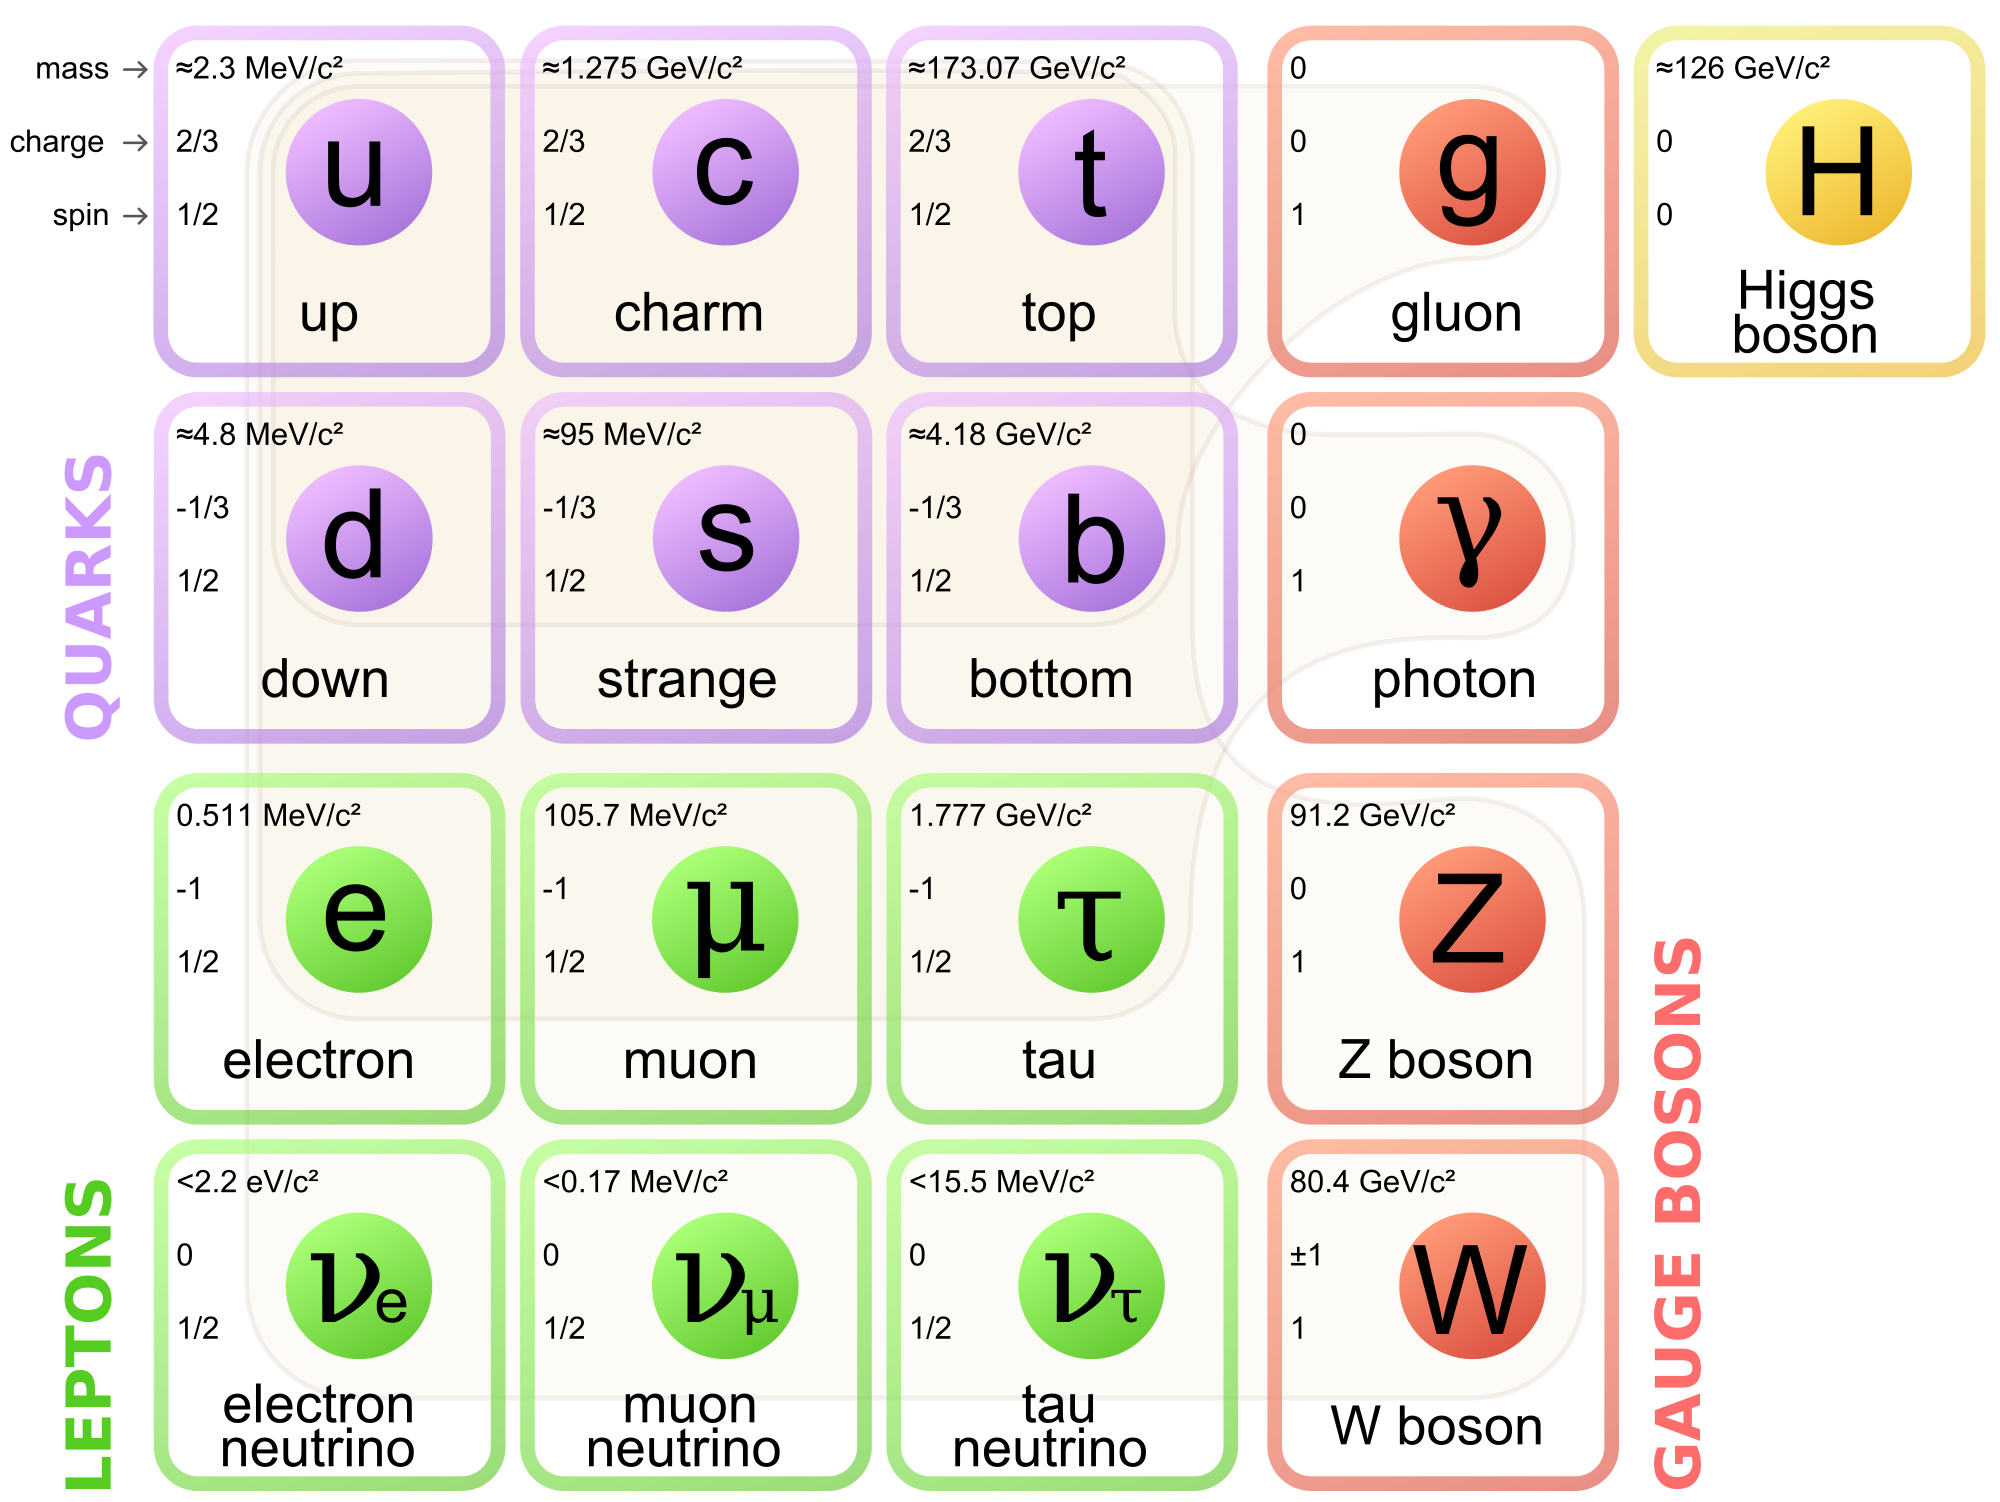
\includegraphics[width=0.9\textwidth]{IntroFigures/TheSM.png}
 \caption{The catalog of particles in the standard model.\label{fig:SMcartoon}}
\end{figure}

The dynamics and kinematics of the SM are controlled by the
Lagrangian density, which in conjunction with the particle content and
force carriers completes the theory. The lagrangian density is
presented below in compact formulation:
\begin{equation}
 \begin{aligned}
        \mathcal{L}_{\mathrm{SM}}& = -\frac{1}{4}B_{\mu\nu}B^{\mu\nu}
        -\frac{1}{4}W^{a}_{\mu\nu}W^{\mu\nu}_{a} - \frac{1}{4}G^{\alpha}_{\mu\nu}G^{\mu\nu}_{\alpha} 
        \qquad \text{gauge terms}\\
        &+\bar{\ell}_{\mathrm{L}}\tilde{\sigma}^{\mu}iD_{\mu}\ell_{\mathrm{L}}
        +\bar{e}_{\mathrm{R}}\sigma^{\mu}iD_{\mu}e_{\mathrm{L}} +
        \bar{\nu}_{\mathrm{R}}\sigma^{\mu}iD_{\mu}\nu_{\mathrm{L}} \qquad \text{lepton kinetic terms}\\
        &+\bar{q}_{\mathrm{L}}\tilde{\sigma}^{\mu}iD_{\mu}q_{\mathrm{L}}
        +\bar{u}_{\mathrm{R}}\sigma^{\mu}iD_{\mu}u_{\mathrm{L}} +
        \bar{d}_{\mathrm{R}}\sigma^{\mu}iD_{\mu}d_{\mathrm{L}} + \qquad \text{quark kinetic terms}\\
        &+\mathcal{L}_{\mathrm{Higgs}} +
        \mathcal{L}_{\mathrm{Yukawa}}\qquad \text{Higgs and Yukawa terms}
       \end{aligned}
\label{eq:theSMlagrangian}
\end{equation}

Where $\ell_{\mathrm{L}}=\begin{pmatrix}e_{\mathrm{L}}\\
  \nu_{\mathrm{L}}\end{pmatrix}$ is the lepton $\mathrm{SU(2)_{L}}$
doublet, $q_{\mathrm{L}}=\begin{pmatrix}u_{\mathrm{L}}\\
  d_{\mathrm{L}}\end{pmatrix}$ is the quark $\mathrm{SU(2)_{L}}$
doublet, $D_{\mu}$ is the corresponding covariant derivative, and
 $\sigma_{mu}$ is the identity and the pauli matrices ($\sigma_{mu} = {1,\sigma^{i}}$).
The $\mathcal{L}_{\mathrm{Higgs}}$ and $\mathcal{L}_{\mathrm{Yukawa}}$
are presented in sections~\ref{higgs} and~\ref{yukawa}, respectively.
Table~\ref{tab:SMGroup} presents the matter field representation in
the SM gauge group.

\begin{table}[htb]
\centering
\large
\begin{tabular}{cccc}
  \hline
  \hline
  field &  $\mathrm{SU(3)_{C}}$ &  $\mathrm{SU(2)_{L}}$ & $\mathrm{U(1)_{Y}}$\\
  \hline                                                        
  $q_{L}$ & $\mathbf{3}$ &  $\mathbf{2}$ & 1/6\\
  $\ell_{L}$ & $\mathbf{1}$ &  $\mathbf{2}$ & -1/2\\
  $u_{R}$ & $\mathbf{\bar{3}}$ &  $\mathbf{1}$ &-2/3\\
  $d_{R}$ & $\mathbf{\bar{3}}$ &  $\mathbf{1}$ &1/3\\
  $e_{R}$ & $\mathbf{1}$ &  $\mathbf{1}$ & 1\\
  $h$ & $\mathbf{1}$ &  $\mathbf{1}$ & 1/2\\
  \hline
  \hline
\end{tabular}
  \caption{\label{tab:SMGroup} Group representation of the matter
    fields in the SM.}
\end{table}
\section{The Higgs Boson and Electroweak Symmetry
  Breaking}\label{higgs}
Gauge theories prohibit -- in order to mantain the local symmetries --  explicit mass terms for the gauge bosons in the SM,
therefore all gauge bosons are massless. Since some of gauge boson in
the SM are massive ($W^{\pm}$,$Z$) there should be a mechanism by
which gauge boson acquire mass. The gauge boson masses in the SM are
realized by the \textit{spontaneous symmetry breaking} of the
$\mathrm{SU(2)_{L}}\times U(1)_{\mathrm{Y}}$ symmetry which induced by the nature of
the Higgs potential~\cite{HIGGES}. The best way to undertand this mechanism (the
Higgs mechanism) is to closely look at the lagrangian density:

\begin{equation}
\label{eq:higgsPotential}
\mathcal{L}_{\mathrm{Higgs}} =
(D^{\mu}\mathbf{\Phi})^{\dagger}(D^{\mu}\mathbf{\Phi}) +
V(\mathrm{\Phi});\hspace{1cm} V(\mathrm{\Phi}) = -\mu^{2}\Phi^{\dagger}\Phi +\lambda(\Phi^{\dagger}\Phi)^{2},
\end{equation}
where $D^{\mu}$ is the covariant derivative; $\Phi$ is a spin-0
complex field, and a $\mathrm{SU(2)_{L}}$ doublet with weak
hypercharge $\mathrm{Y} = 1/2$. The field is more easily represented
as a $\mathrm{SU(2)_{L}}$ doublet in the following fashion:
\begin{equation}
\label{eq:higgdoublet}
\Phi = \begin{pmatrix} \phi^{+}\\
  \phi^{0}\end{pmatrix}.
\end{equation}

When $\mu^{2} > 0$ the potential ($V(\Phi)$) has the commonly known
``Mexican hat'' shape, shown in Figure~\ref{fig:MexHat}, whith a minimum which does not preserve the
original $\mathrm{SU(2)_{L}}\times U(1)_{\mathrm{Y}}$
symmetry. Therefore the scalar field acquires a non-zero
\textit{vacuum expectation value (vev)}:
\begin{equation}
\label{eq:vev}
\langle \Phi \rangle \equiv \langle 0 | \Phi | 0\rangle = \frac{1}{\sqrt{2}}U(x) \begin{pmatrix} 0\\
  v\end{pmatrix}; \hspace{1cm}v = \sqrt{\frac{\mu^{2}}{\lambda}},
\end{equation}

\begin{figure}
 \centering
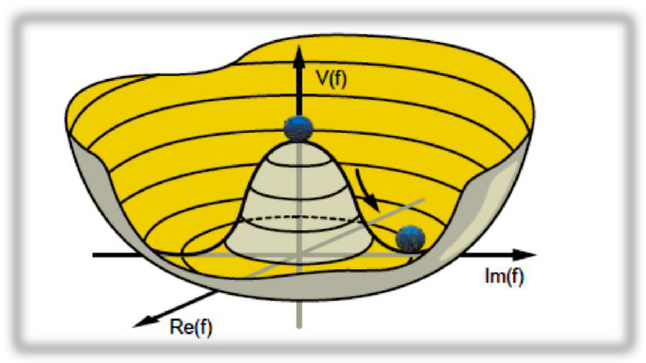
\includegraphics[width=0.9\textwidth]{IntroFigures/MexicanHat.png}
 \caption{The shape of the Higgs potential (``Mexican hat''). The
   degeneracy of the potential is observed along the azimuthal angle\label{fig:MexHat}}
\end{figure}

where $U(x)$ is a unitary transformation that transforms the field
into the degenerate solution. An important consequence is that the
\textit{vev} of field preserves a $U(1)$ symmetry from the original
$\mathrm{SU(2)_{L}}\times U(1)_{\mathrm{Y}}$ symmetry of the
lagrangian. Therefore the full electroweak symmetry of the SM
($\mathrm{SU(2)_{L}}\times U(1)_{\mathrm{Y}}$) is spontaneously broken
to $U(1)_{\mathrm{EM}}$.

This spontaneous breaking of the $\mathrm{SU(2)_{L}}\times
U(1)_{\mathrm{Y}}$ symmetry is responsible for the appearance of
masses to 3 of the four gauge bosons in the electroweak sector, this
is called: the Higgs mechanism. The masses become apparent when
replacing the \textit{vev} into the Higgs kinetic term in the
lagrangian:

\begin{equation}
\label{eq:HiggsMass}
(D^{\mu}\Phi)^{\dagger}(D^{\mu}\Phi) \rightarrow (\partial_{\mu}
-igA_{\mu}^{a}\tau^{a} - ig^{\prime}B_{\mu})^{\dagger}(\partial_{\mu}
-igA_{\mu}^{a}\tau^{a} - ig^{\prime}B_{\mu}) 
\end{equation}
\section{Fermion Masses}\label{yukawa}
\chapter{Supersymetry and Naturalness}
\chapter{Dark Matter and Weakly Interacting Particles}



AAAAAAAAAAAAAAAAAAAAA~\cite{vandeHulst,Rubin:1980zd}
\section{The Large Hadron Collider}
The CERN Large Hadron Collider (LHC) is a two-ring superconducting
accelerator and collider with 27 km of circumference, which is located
in the tunnel constructed for the CERN Large Electron-Positron
Collider (LEP). The tunnel lies between 45 m and 170 m below the
surface on an incliend plane (1.41\% slope) towards Lake L\`eman and
spans between the French and Swiss border close to Geneva. The layout
of the tunnel is such that contains 8 arc sections that spans most of
the circumference and 8 straight sections where the experimental halls
are located. 

The LHC is a particle-particle collider -- in its most common
configuration it collides protons -- with a designed center-of-mass
energy of 14\TeV. In order to achieve such high energies, the LHC uses
the existing CERN facilities to gradually increase the energy of the
protons. Everything starts with a bottle of compressed hydrogen gas,
then, hydrogen atoms are fed into the source chamber of the linear
accelerator, where an electric field strips off their
electrons. The resulting protons are then injected into the linear
accelaretor, Linac 2, which is the first step in the
accelerator chain and boosts the
protons energy up to 50\MeV. The accelated proton beam is then divided
into 4 (to increase its intensity) and enters the second stage of
acceleration, this occurs in the Proton Synchroton Booster (PSB),
where protons are now accelerated to 1.4\GeV. Subsequently, the proton beam is
recombined and sent to the Proton Synchrotron (PS), which increases
the energy to 25\GeV, followed by the Super Proton Synchrotron (SPS),
which brings the beam energy to 450\GeV.

Finally, the proton beam is transfered to the two beam pipes of the
LHC. The beams circulate in opposite directions. The LHC filling time
is 4 minutes and 20 seconds, but it takes around 20 minutes for the
protons to reach their maximum energy. Figure~\ref{fig:cernAcc} shows
the CERN accelerator complex just described.
\begin{figure}
 \centering
 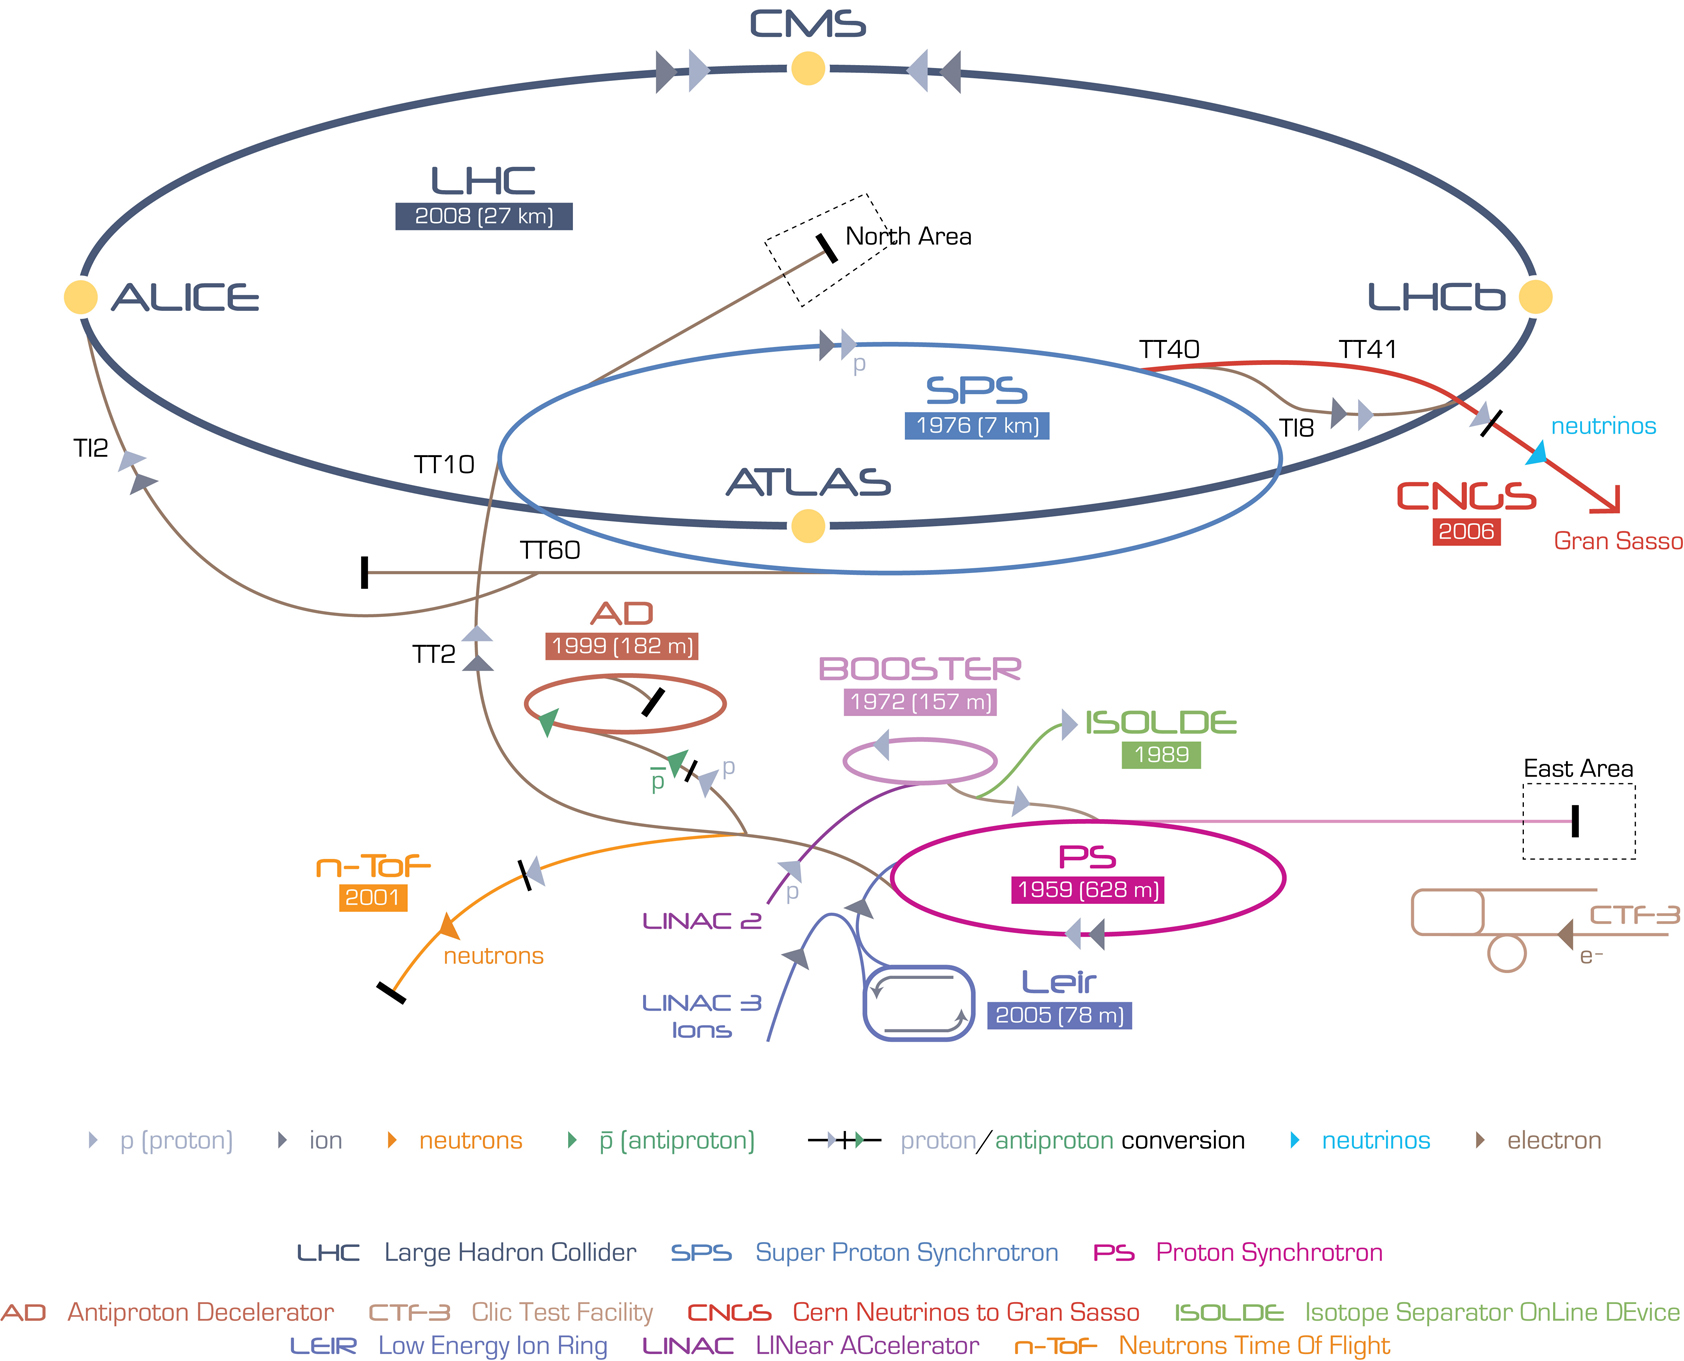
\includegraphics[width=0.9\textwidth]{LHC_fig/Cern-Accelerator-Complex.jpg}
 \caption{The CERN accelerator complex.\label{fig:cernAcc} }
\end{figure}
At this point, the two beams are brought to collide at the four interaction points (IP) in the straight
sections where the LHC's experiments are located. There are two main
purpose experiments located in diametrical opposite locations, the
ATLAS experiment is located at point 1 and the CMS experiment is
located at point 1. There are also two specialized experiments; the
LHCb experiment, which studies B-hadron physics, and the ALICE
experiment, which specializes in studying heavy ion collisions (another type of
collision possible at the LHC). Figure~\ref{fig:LHC} shows an
squematic layout of the LHC.
\begin{figure}
 \centering
 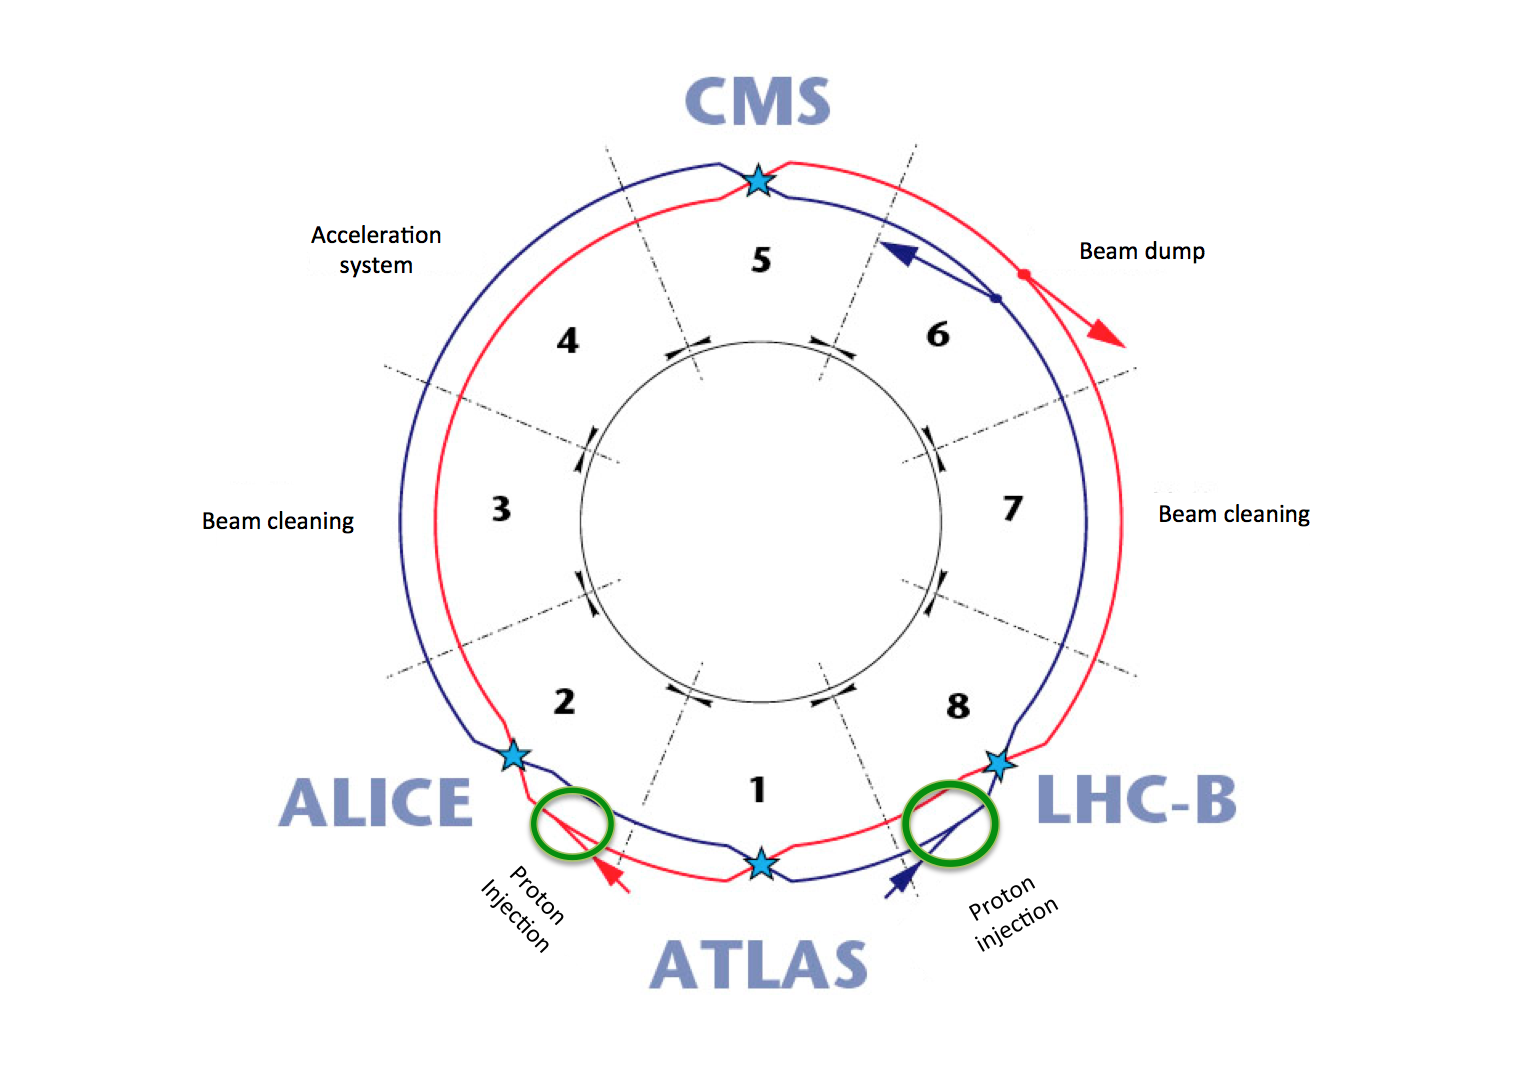
\includegraphics[width=0.9\textwidth]{LHC_fig/LHC_layout.png}
 \caption{The CERN Large Hadron Collider schematic layout.\label{fig:LHC} }
\end{figure}
Due to the small diameter of the tunnel in the arcs
(3.7~m), which complicates the installation of two separate proton
rings, the LHC uses a twin-bore magnet design, proposed in 1971 by
John Blewett at the Brookhaven National Laboratory
(BNL)~\cite{JBlewett} as a cost-saving alternative. 

Since the usage of superconducting magnets a the Intersecting  Storage
Rings at CERN, particle colliders have used them as the default
technology for their operation. However, the main difference is that the LHC's
superconducting magnets operate at a tempareture lower (below 2~K) than the
standard superconducting magnets in other particle colliders
(4-5~K). The LHC ring accomodates 1,232 NbTi main dipole magnets,
cooled down to 1.9 K by using superfluid helium; they operate at fields
above 8~T. The twin-bore desing allow for a common nonmagnetic collar
and iron yoke, as well as common cryogenic system. The core of the
dipole magnet system is enclosed by a cylindrical alloyed low-carbon steel vacuum vessel with an outer diameter of 914\mm and a wall
thickness of 12\mm. Figures~\ref{fig:magnet1} and~\ref{fig:magnet2} show a cross sectional
view and a 3-dimensional visualization of the main dipole magnet
system, respectively.
\begin{figure}
 \centering
 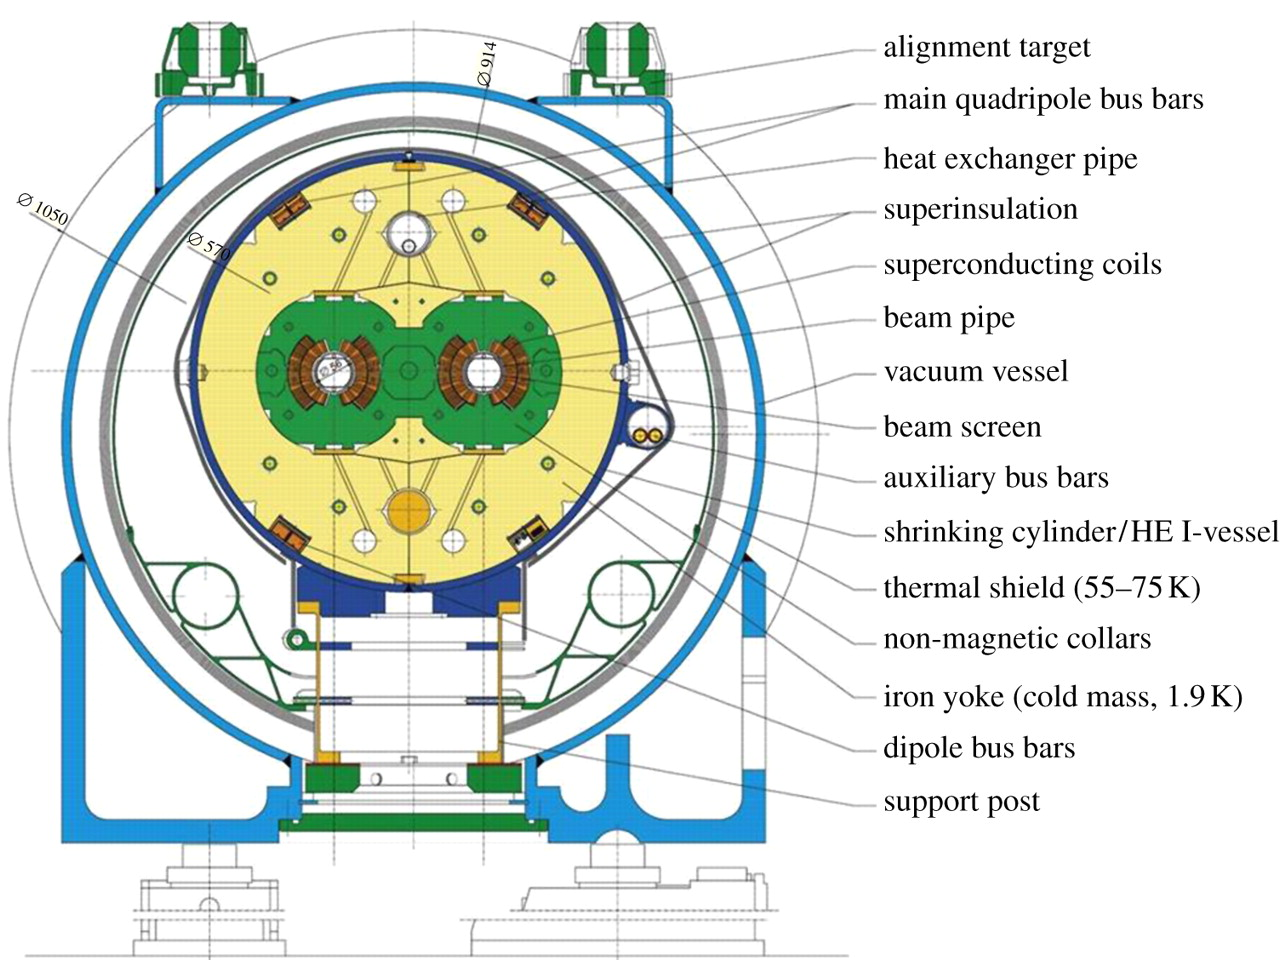
\includegraphics[width=0.9\textwidth]{LHC_fig/ColdMassMagnet.jpg}
 \caption{An schematic cross sectional view of the LHC dipole magnet.\label{fig:magnet1} }
\end{figure}
\begin{figure}
 \centering
 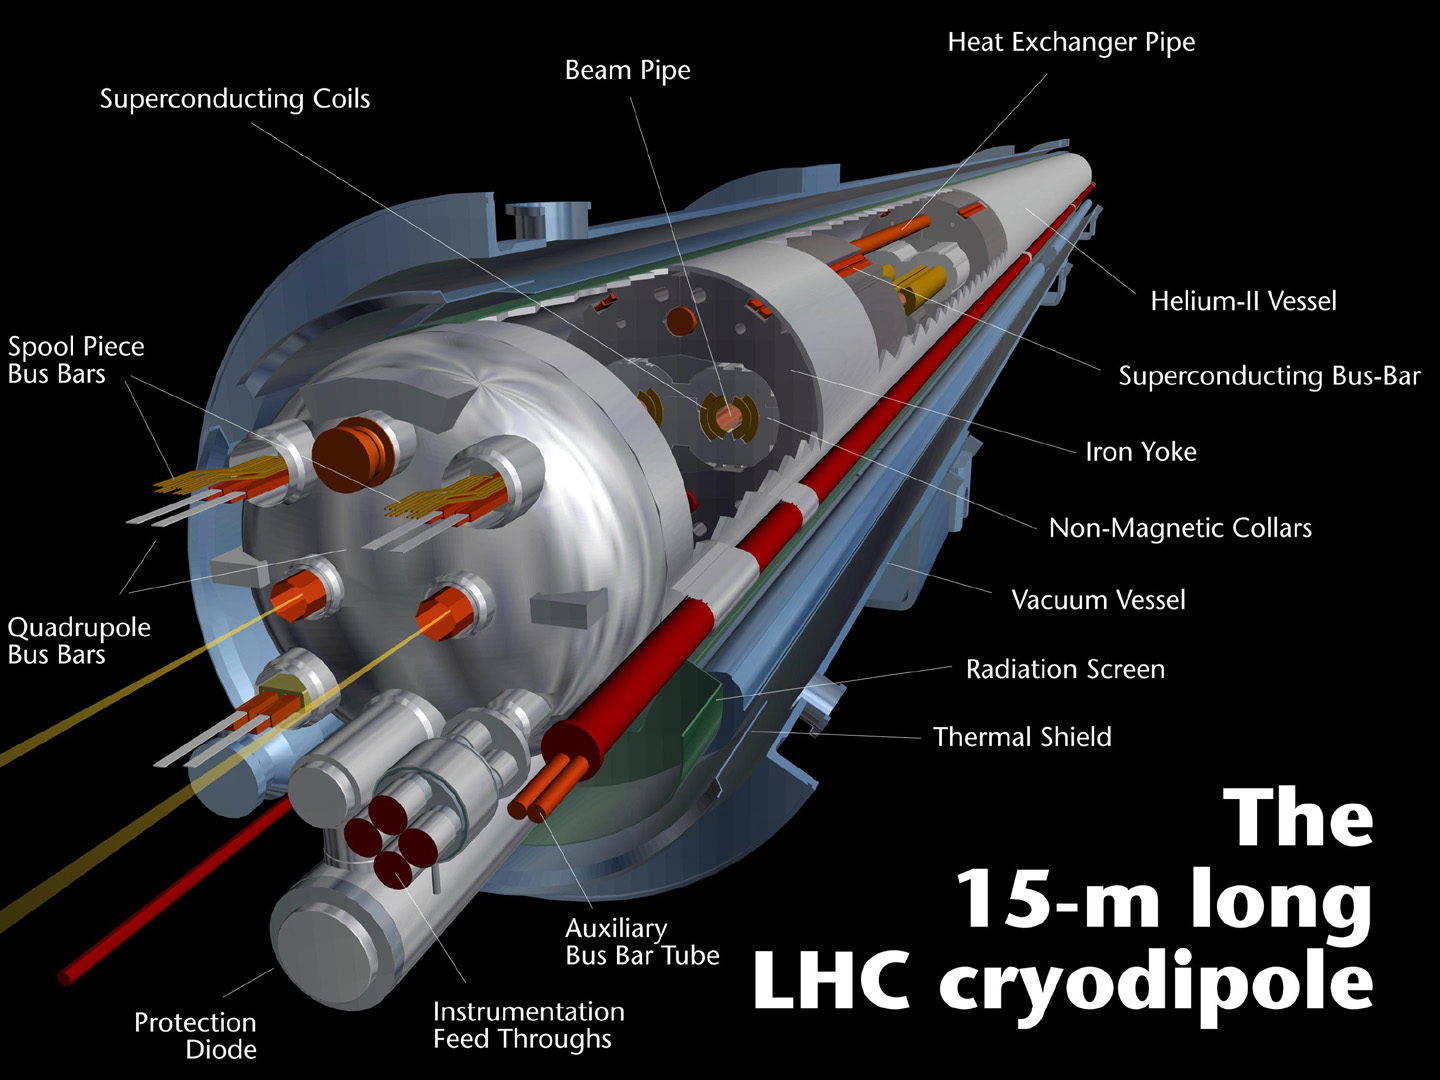
\includegraphics[width=0.9\textwidth]{LHC_fig/cryodipole.jpg}
 \caption{An 3D visualization of a LHC dipole magnet.\label{fig:magnet2} }
\end{figure}

The goal of the LHC program is to reveal the nature of new
physics. The high-energy collision (14\TeV) are a key ingredient to probe new
physics, since new physics could just be present at that energy
scale. However, it is by no means the only ingredient; new physics
will likely have smaller cross sections than that of the known SM
processes and therefore a large number of proton-proton collision is
needed. The number of events for a particular physics process $N_{exp}$
generated in the LHC is the product of the experimental cross section $\sigma_{exp}$
and the integrated luminosity, i.e.
\begin{equation}
N_{exp} = \sigma_{exp}\int\mathcal{L}(t)dt.
\end{equation}
Where $\mathcal{L}(t)$ is the instantaneous luminosity, which depends
on the LHC beam parameters and can be written as\cite{LHCbeamParam}:
\begin{equation}
\mathcal{L}(t) = \frac{N^{2}_{b}n_{b}f_{rev}\gamma_{r}}{4\pi\epsilon_{n}\beta^{*}},
\end{equation}
where $N_{b}$ is the number of particles per bunch, $n_{b}$ is the
number of bunches per beam, $f_{rev}$ is the revolution frequency,
$\gamma_{r}$ is the relativistic factor, $\epsilon_{n}$ is the
normalized transverse beam emittance, $\beta^{*}$ is the transverse
size of the beam at the IP, and $F$ is the geometric luminosity
reduction factor due to the crossing angle at the IP:
\begin{equation}
F=\left(1+\left(\frac{\theta_{c}\sigma_{z}}{2\sigma^{*}}\right)\right)^{-1/2}
\end{equation}
In the last expression, $\theta_{c}$ is the full crossing angle at the
IP, $\sigma_{z}$ is the rms bunch length, and $\sigma^{*}$ is the
transverse rms beam size at the IP. The designed peak luminosity to be
deliverd the ATLAS and CMS is $\mathcal{L}(t) = 10^{34}$~cm$^-2$~s$^{-1}$.  
Figure~\ref{fig:lumi} shows the integrated luminosity
received by the CMS experiment from 2007 to 2016. 
\begin{figure}
 \centering
 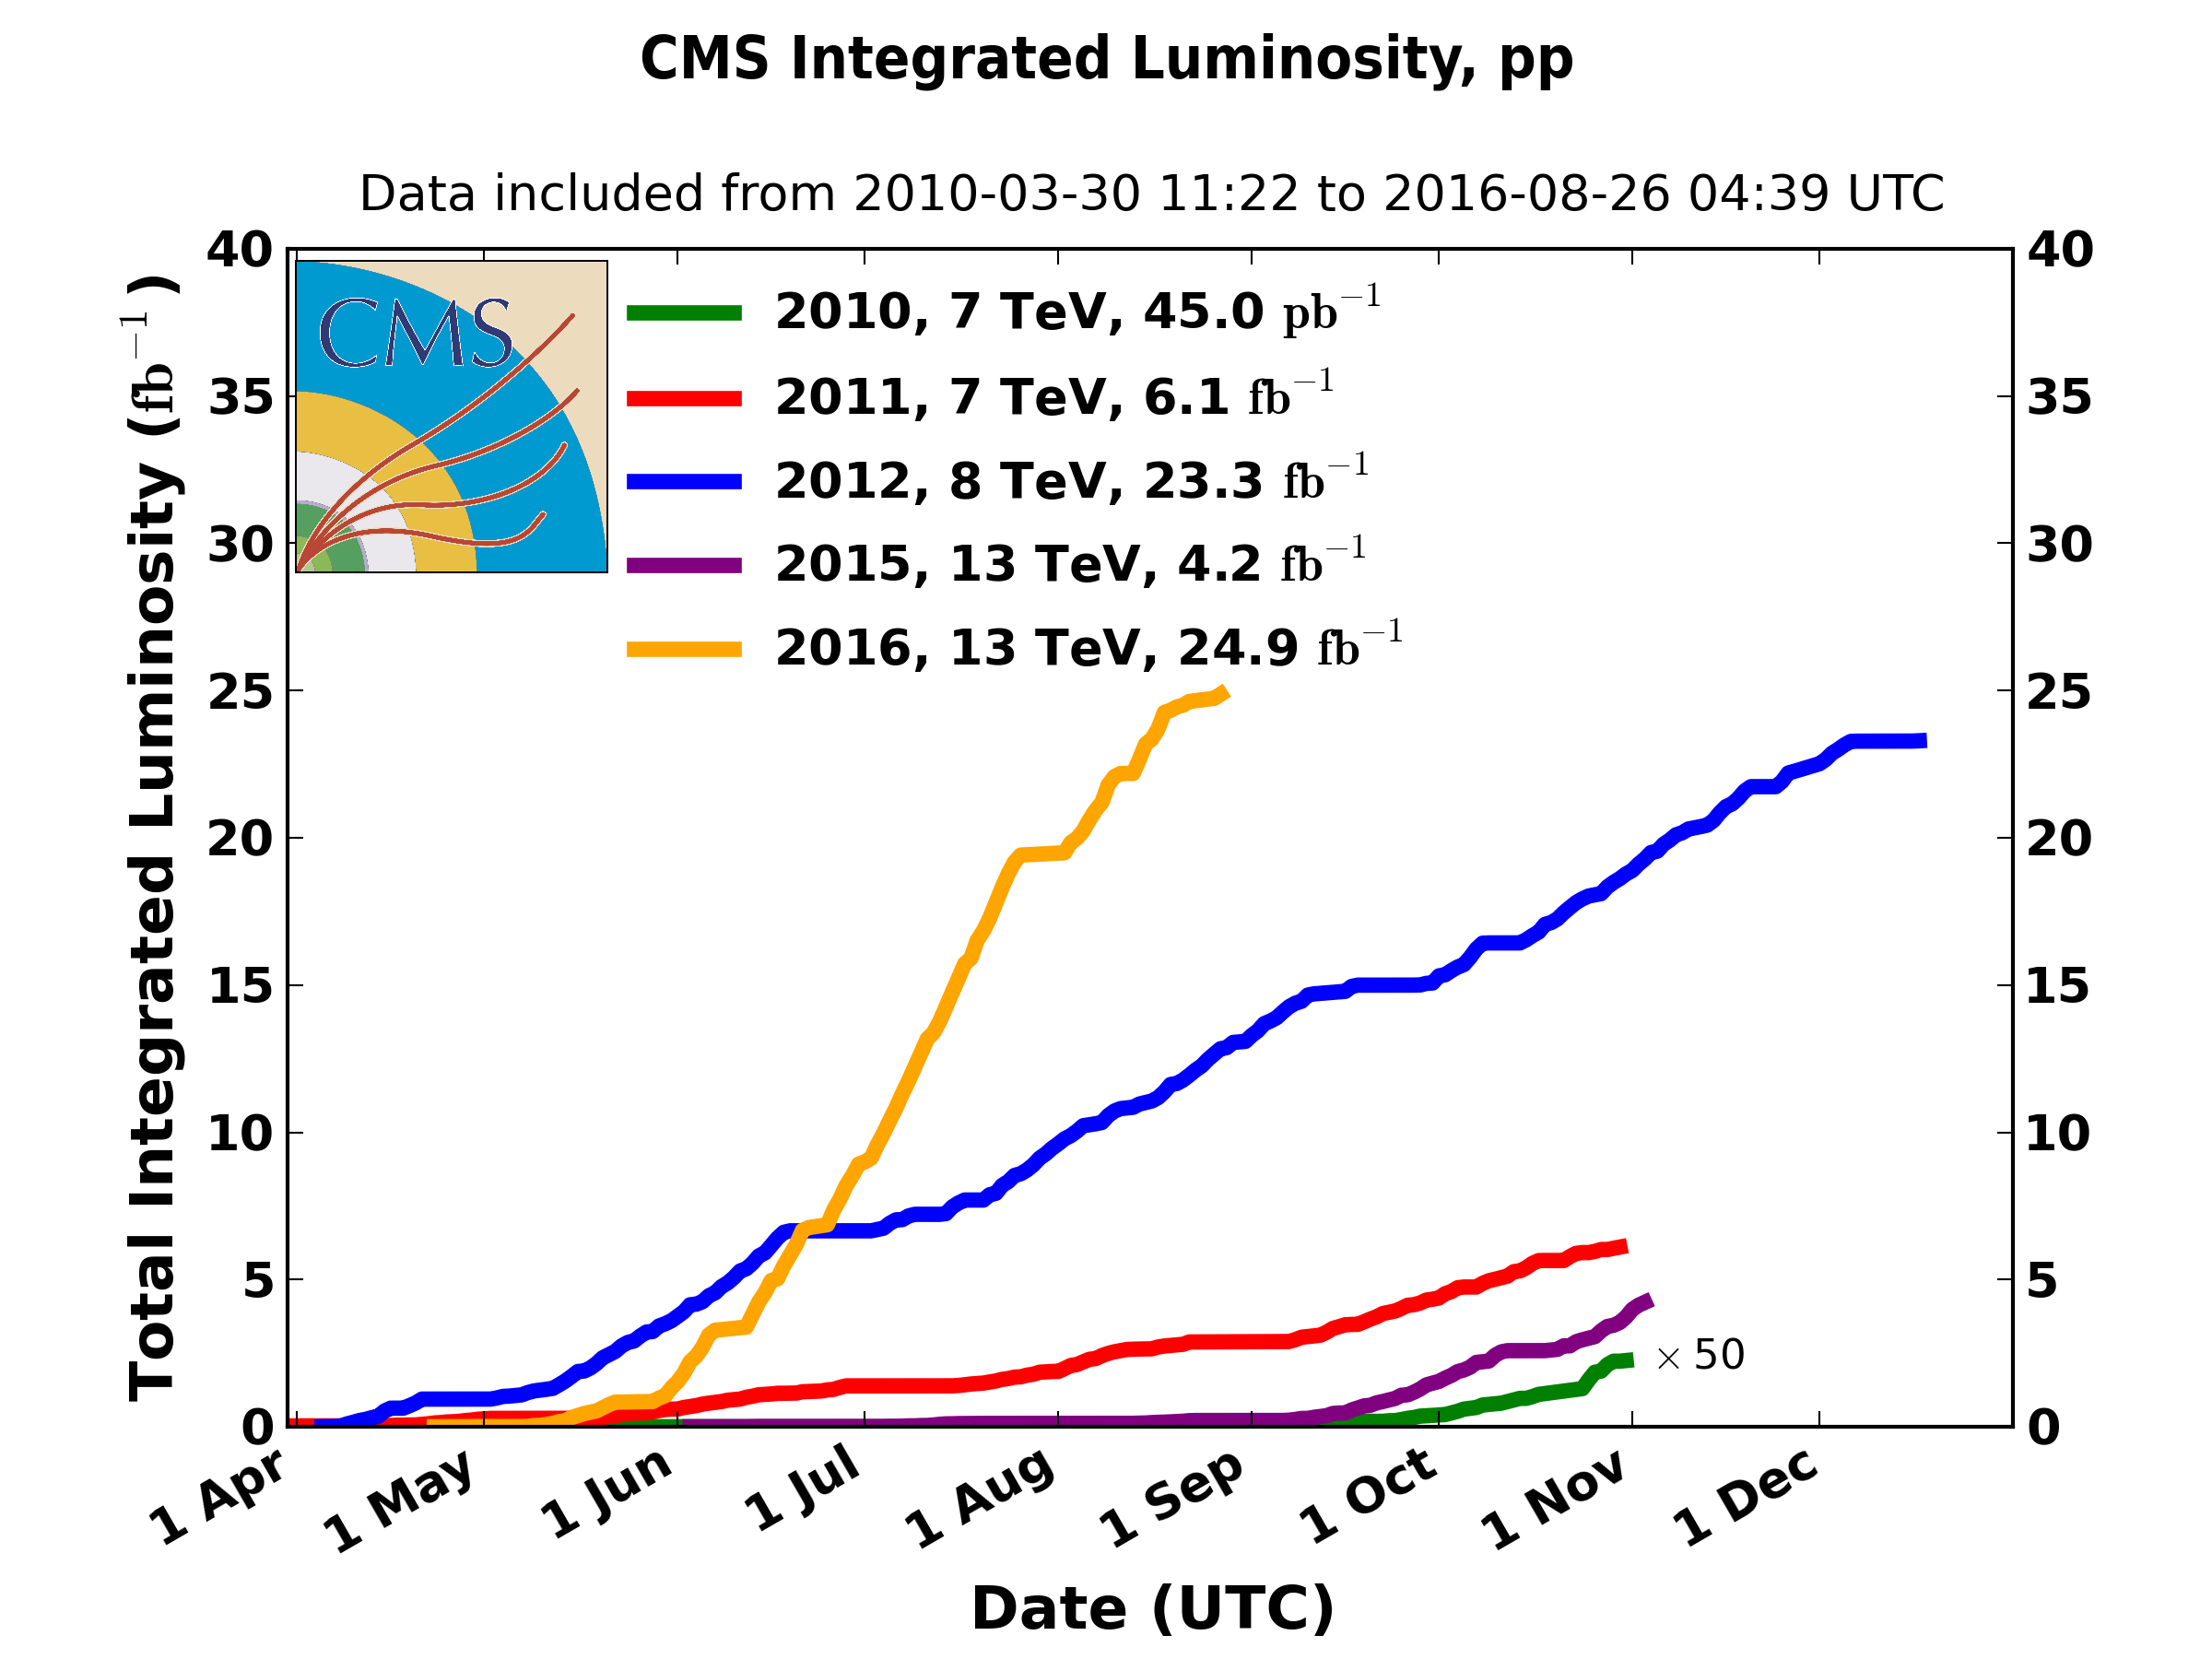
\includegraphics[width=0.9\textwidth]{LHC_fig/int_lumi_cumulative_pp_2.png}
 \caption{Intregated luminosity received by the CMS experiment during the LHC operation.\label{fig:lumi} }
\end{figure}

The Compact Muon Solenoid (CMS) detector operates at the LHC at CERN. It was designed to operate in proton-proton (and lead-lead)
collisions at a center-of-mass energy of 14\TeV (5.5\TeV) and at
luminosities up to 10$^{34}$cm$^{-2}$s$^{-1}$
(10$^{27}$cm$^{-2}$s$^{-1}$). The CMS has cilindrical geometry and
its dimensions are a length of 21.5 m, a diameter of 14.6, and a total
weight of 12,500 tons. At the heart of the CMS detector system
lies a 4\unit{T} magnetic field produced by a large-bore superconducting
solenoid which encloses a silicon -- pixel and strips -- tracker, a homogeneous
lead-tungstate crystal electromagnetic calorimeter, and a brass-scintillator
sampling hadron calorimeter. Outside the superconducting solenoid lies
an iron yoke for magnetic flux-return instrumented with four stations
for muon detection. Forward sampling calorimeters extend the rapidity
coverage up to $\eta < 5$ and thus ensure good
hemiticity. Figure~\ref{fig:cmsDetector} shows an schematic representation
of the CMS detector and Figure~\ref{fig:cmsSlice} shows a cartoon
with a cross-sectional-slice view of the CMS detector along with
different particle detections.
\begin{figure}
 \centering
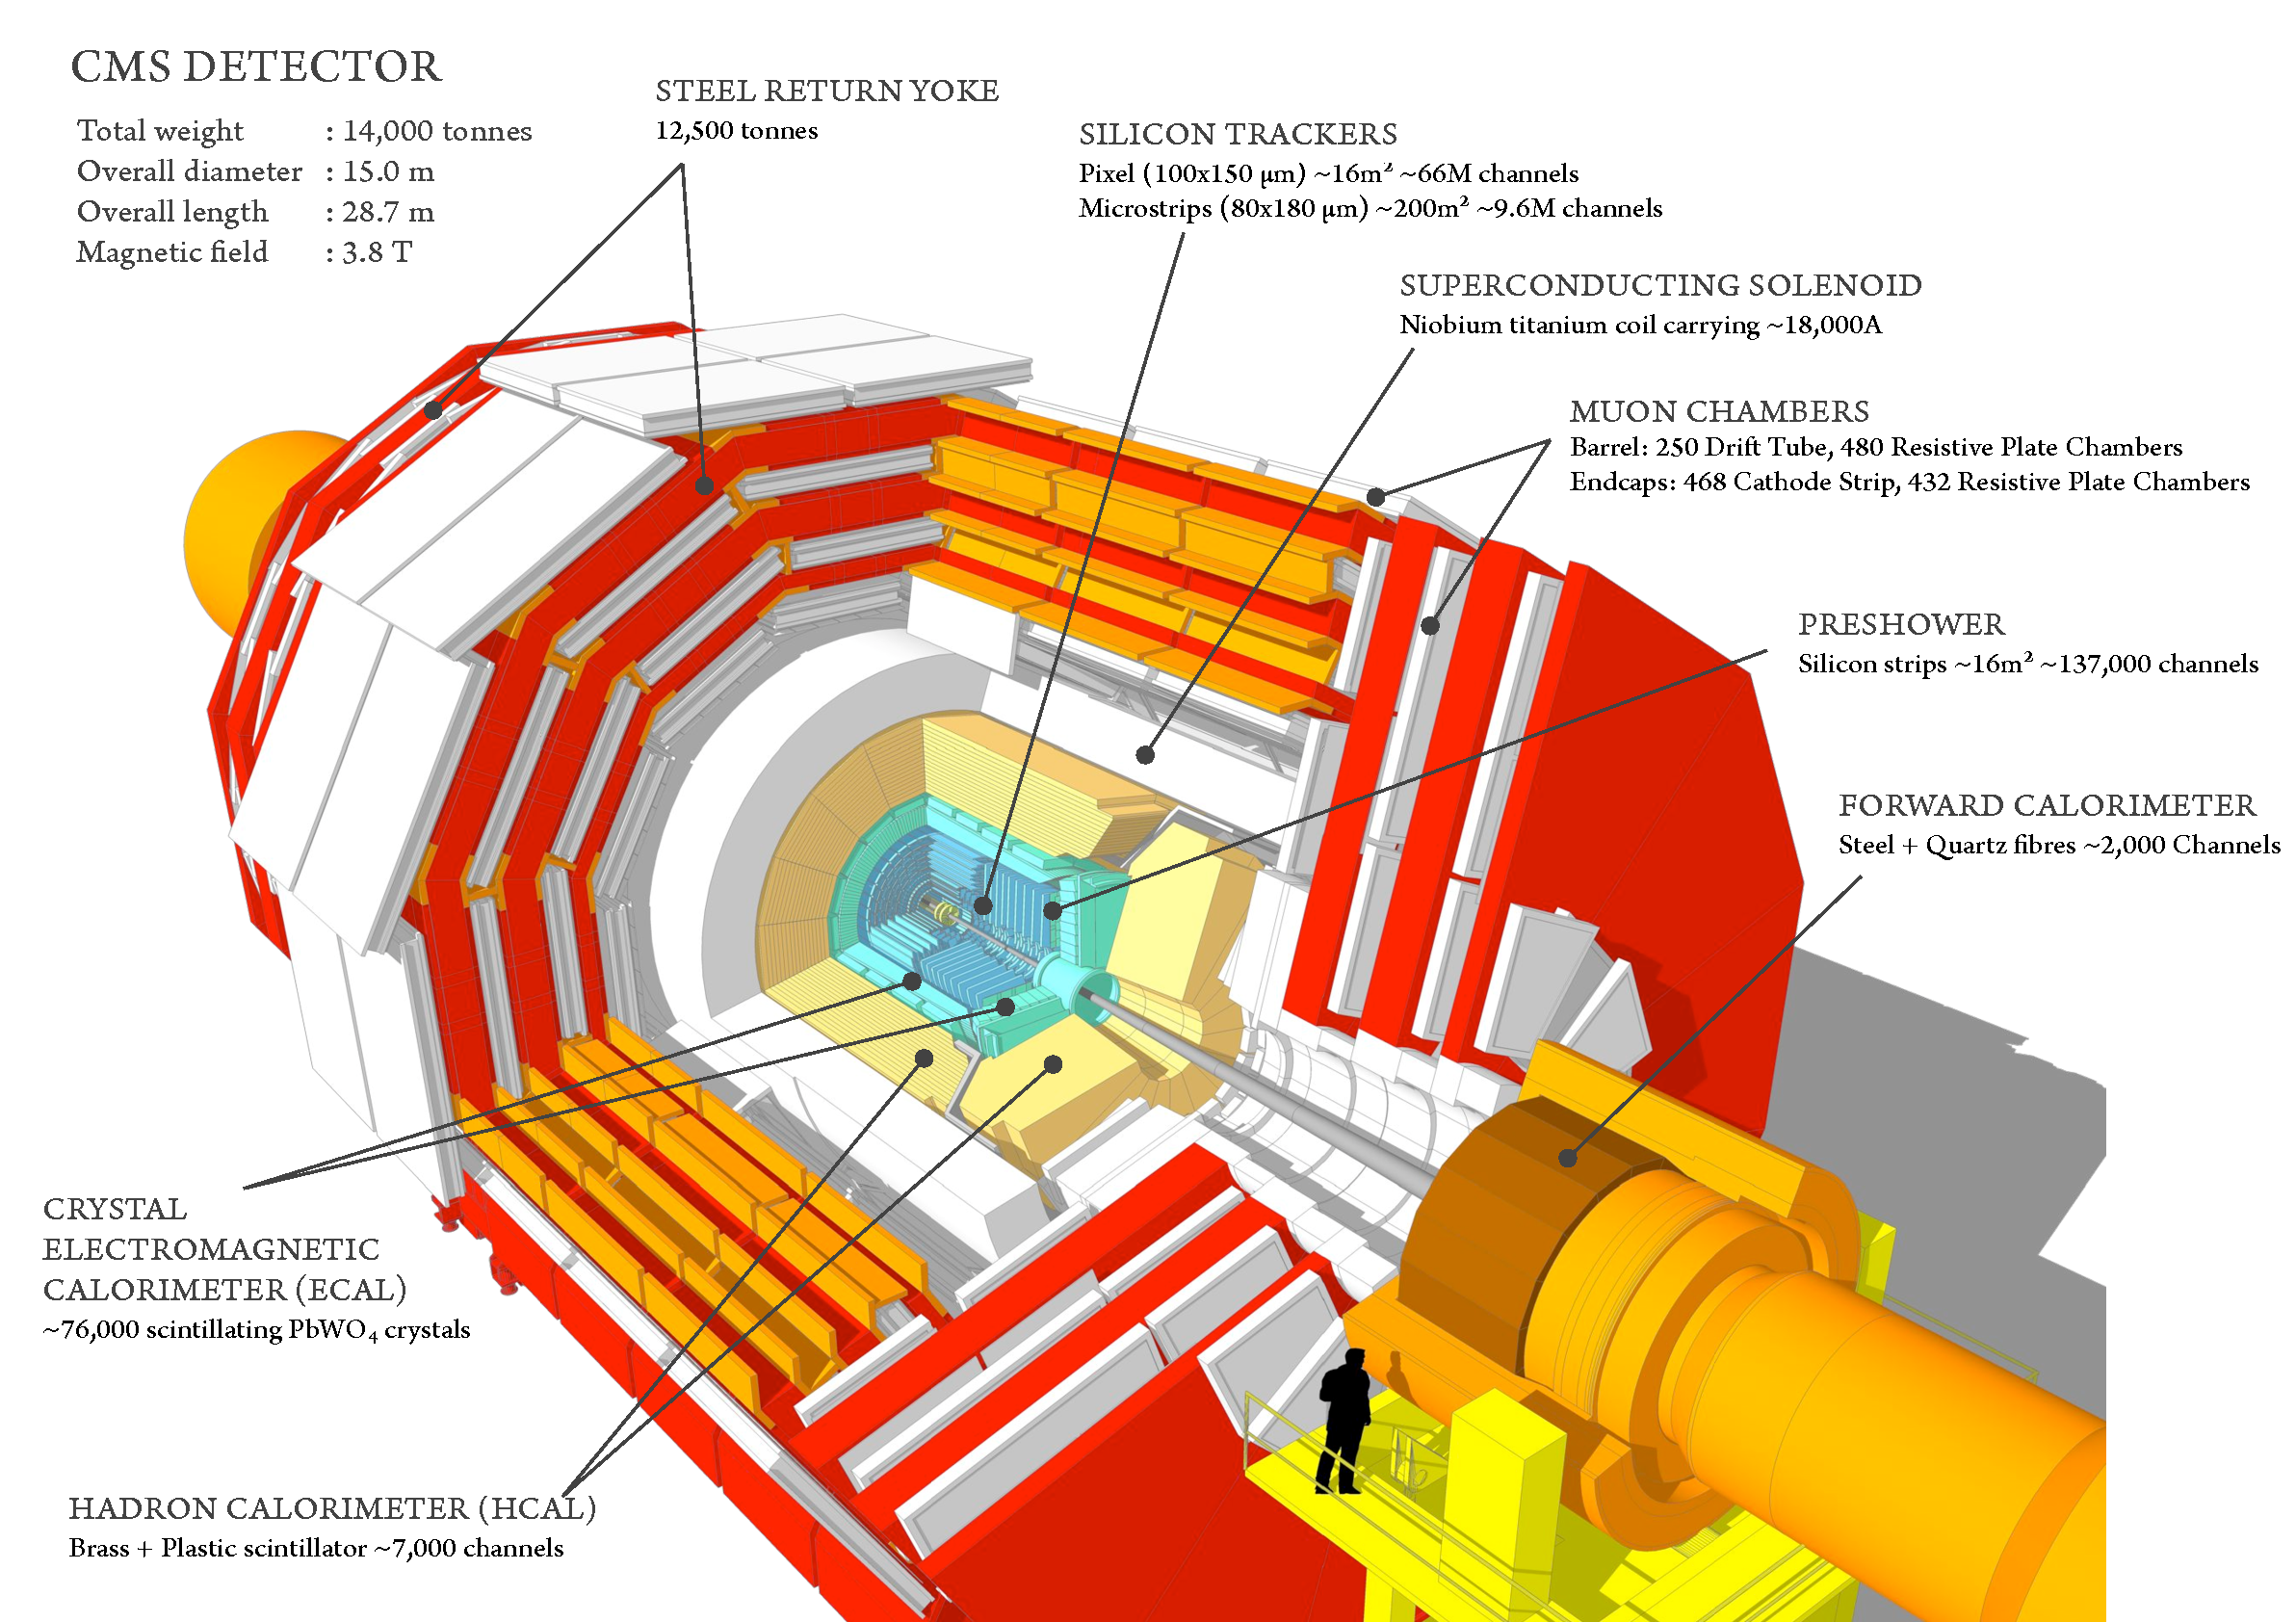
\includegraphics[width=0.99\textwidth]{CMS_DetectorFigures/cms_detector.png}
 \caption{A perspective view of the CMS detector.\label{fig:cmsDetector}}
\end{figure}
\begin{figure}
 \centering
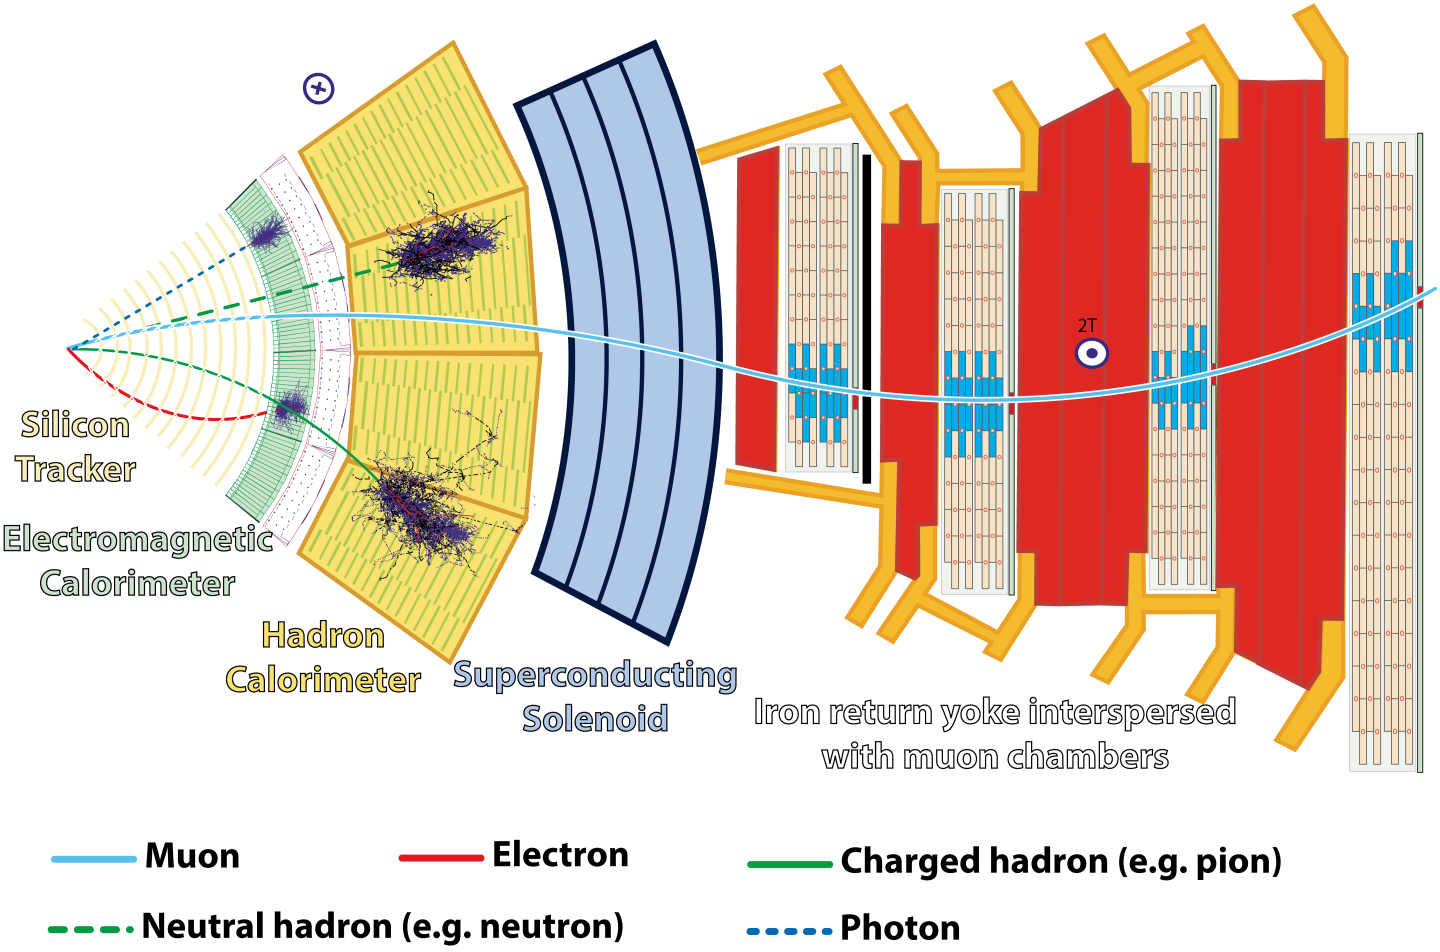
\includegraphics[width=0.99\textwidth]{CMS_DetectorFigures/CMSslice.png}
 \caption{A cross-sectional-slice view of the CMS detector. The
   different components of the detector are clearly labeled and
   different particle detections are depicted.\label{fig:cmsSlice}}
\end{figure}

This chapter presents an introduction to the CMS detector systems and
reconstruction algorithms. It is by no means a complete picture of the
CMS detector and its mostly based on Ref.~\cite{Chatrchyan:2008zzk}.
\section{The Tracker System}
The tracker is the innermost system of the CMS detector.
It was designed to measure efficiently and precisely the trajectories
of charged particles coming from the interaction points, as well as to
provide a precise reconstruction of the secondary vertices at each
bunch crossing. When running at the LHC designed conditions, every
buch crossing, i.e 25 ns, the number of proton-proton collision will
be about 20 and they will produce an average number of particles of about
1000. These conditions and the above requirements implied a highly granular and fast
response design. That being said, this design due to its high power
consumption requires an efficient cooling system which in turn is in
conflict with the goal of minimizing the material budget and thus
reduce unwanted interactions. In addition, the harsh radiation
environment that will deteriorate the detector performance posed
further challenges in its construction. Therefore, the system --
silicon sensors, readout, mechanical structures, granularity, etc --
was designed to operate for 10 year and satisfying the considerations
listed above. The CMS tracker is composed of three layers of pixels
detectors up to a radius of 10.2 cm, a 10-layer silicon strip tracker
up to a radious of 1.1 m, two endcap disks at each side of the barrel pixel detectors, 3
endcap disks at each side of the inner region of the strips (up to a
radius of 55 cm), and finally 9 disks covering the $|z|$ > 120 cm
regions starting a radious of 55 cm. More details about the tracker
layout will be given below and are summarized in
Figure~\ref{fig:trackerlayout}. The tracker covers up to
pseudorapidities of $|eta| < 2.5$ with a about 200 m$^2$ of active
silicon area implemented. The material budget of the CMS tracker is
shown in Figure~\ref{fig:materialBudget}. As it can be seen the most
heavily implemented pseudorapidity is found to be at $|\eta|\approx$ 1.4.
\begin{figure}
 \centering
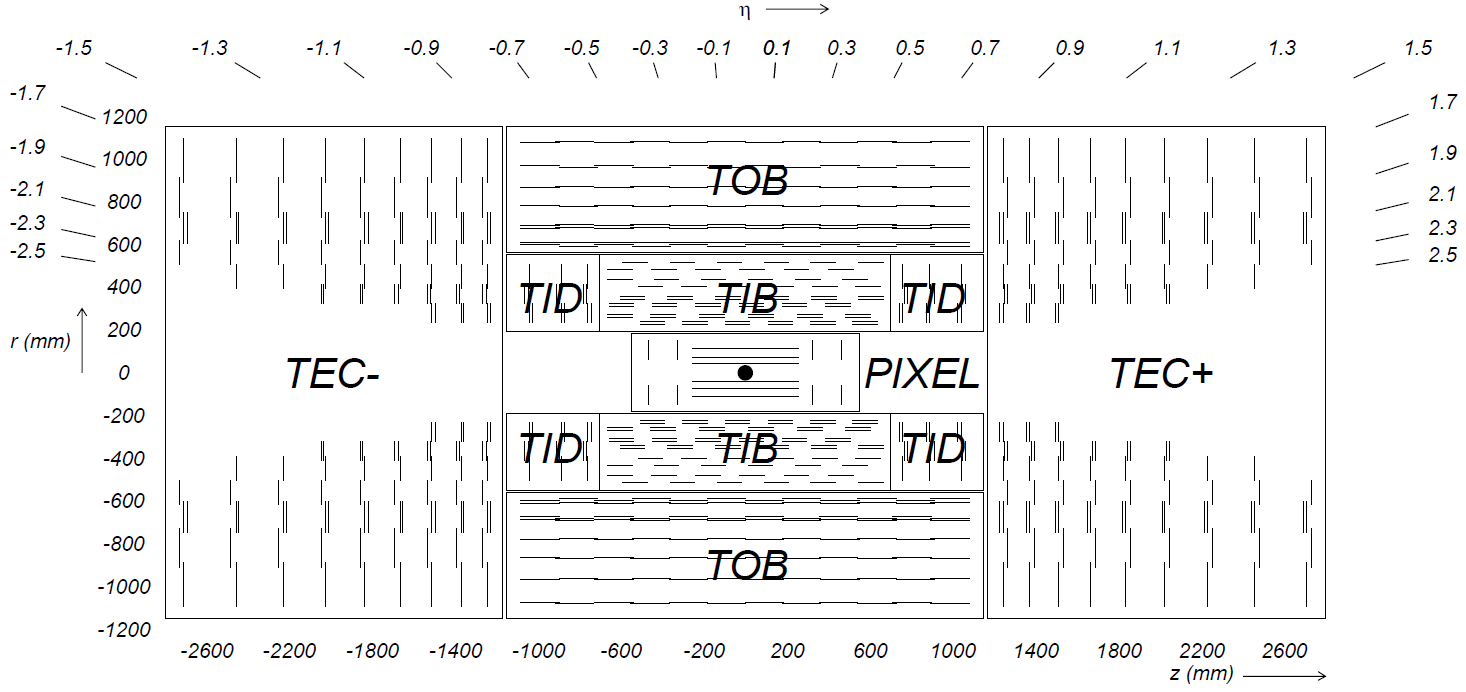
\includegraphics[width=0.99\textwidth]{CMS_DetectorFigures/TrackerLayout.png}
 \caption{A cross-sectional view of the silicon tracker layout. The
   different subsytems are clearly labeled.\label{fig:trackerlayout}}
\end{figure}
\begin{figure}
 \centering
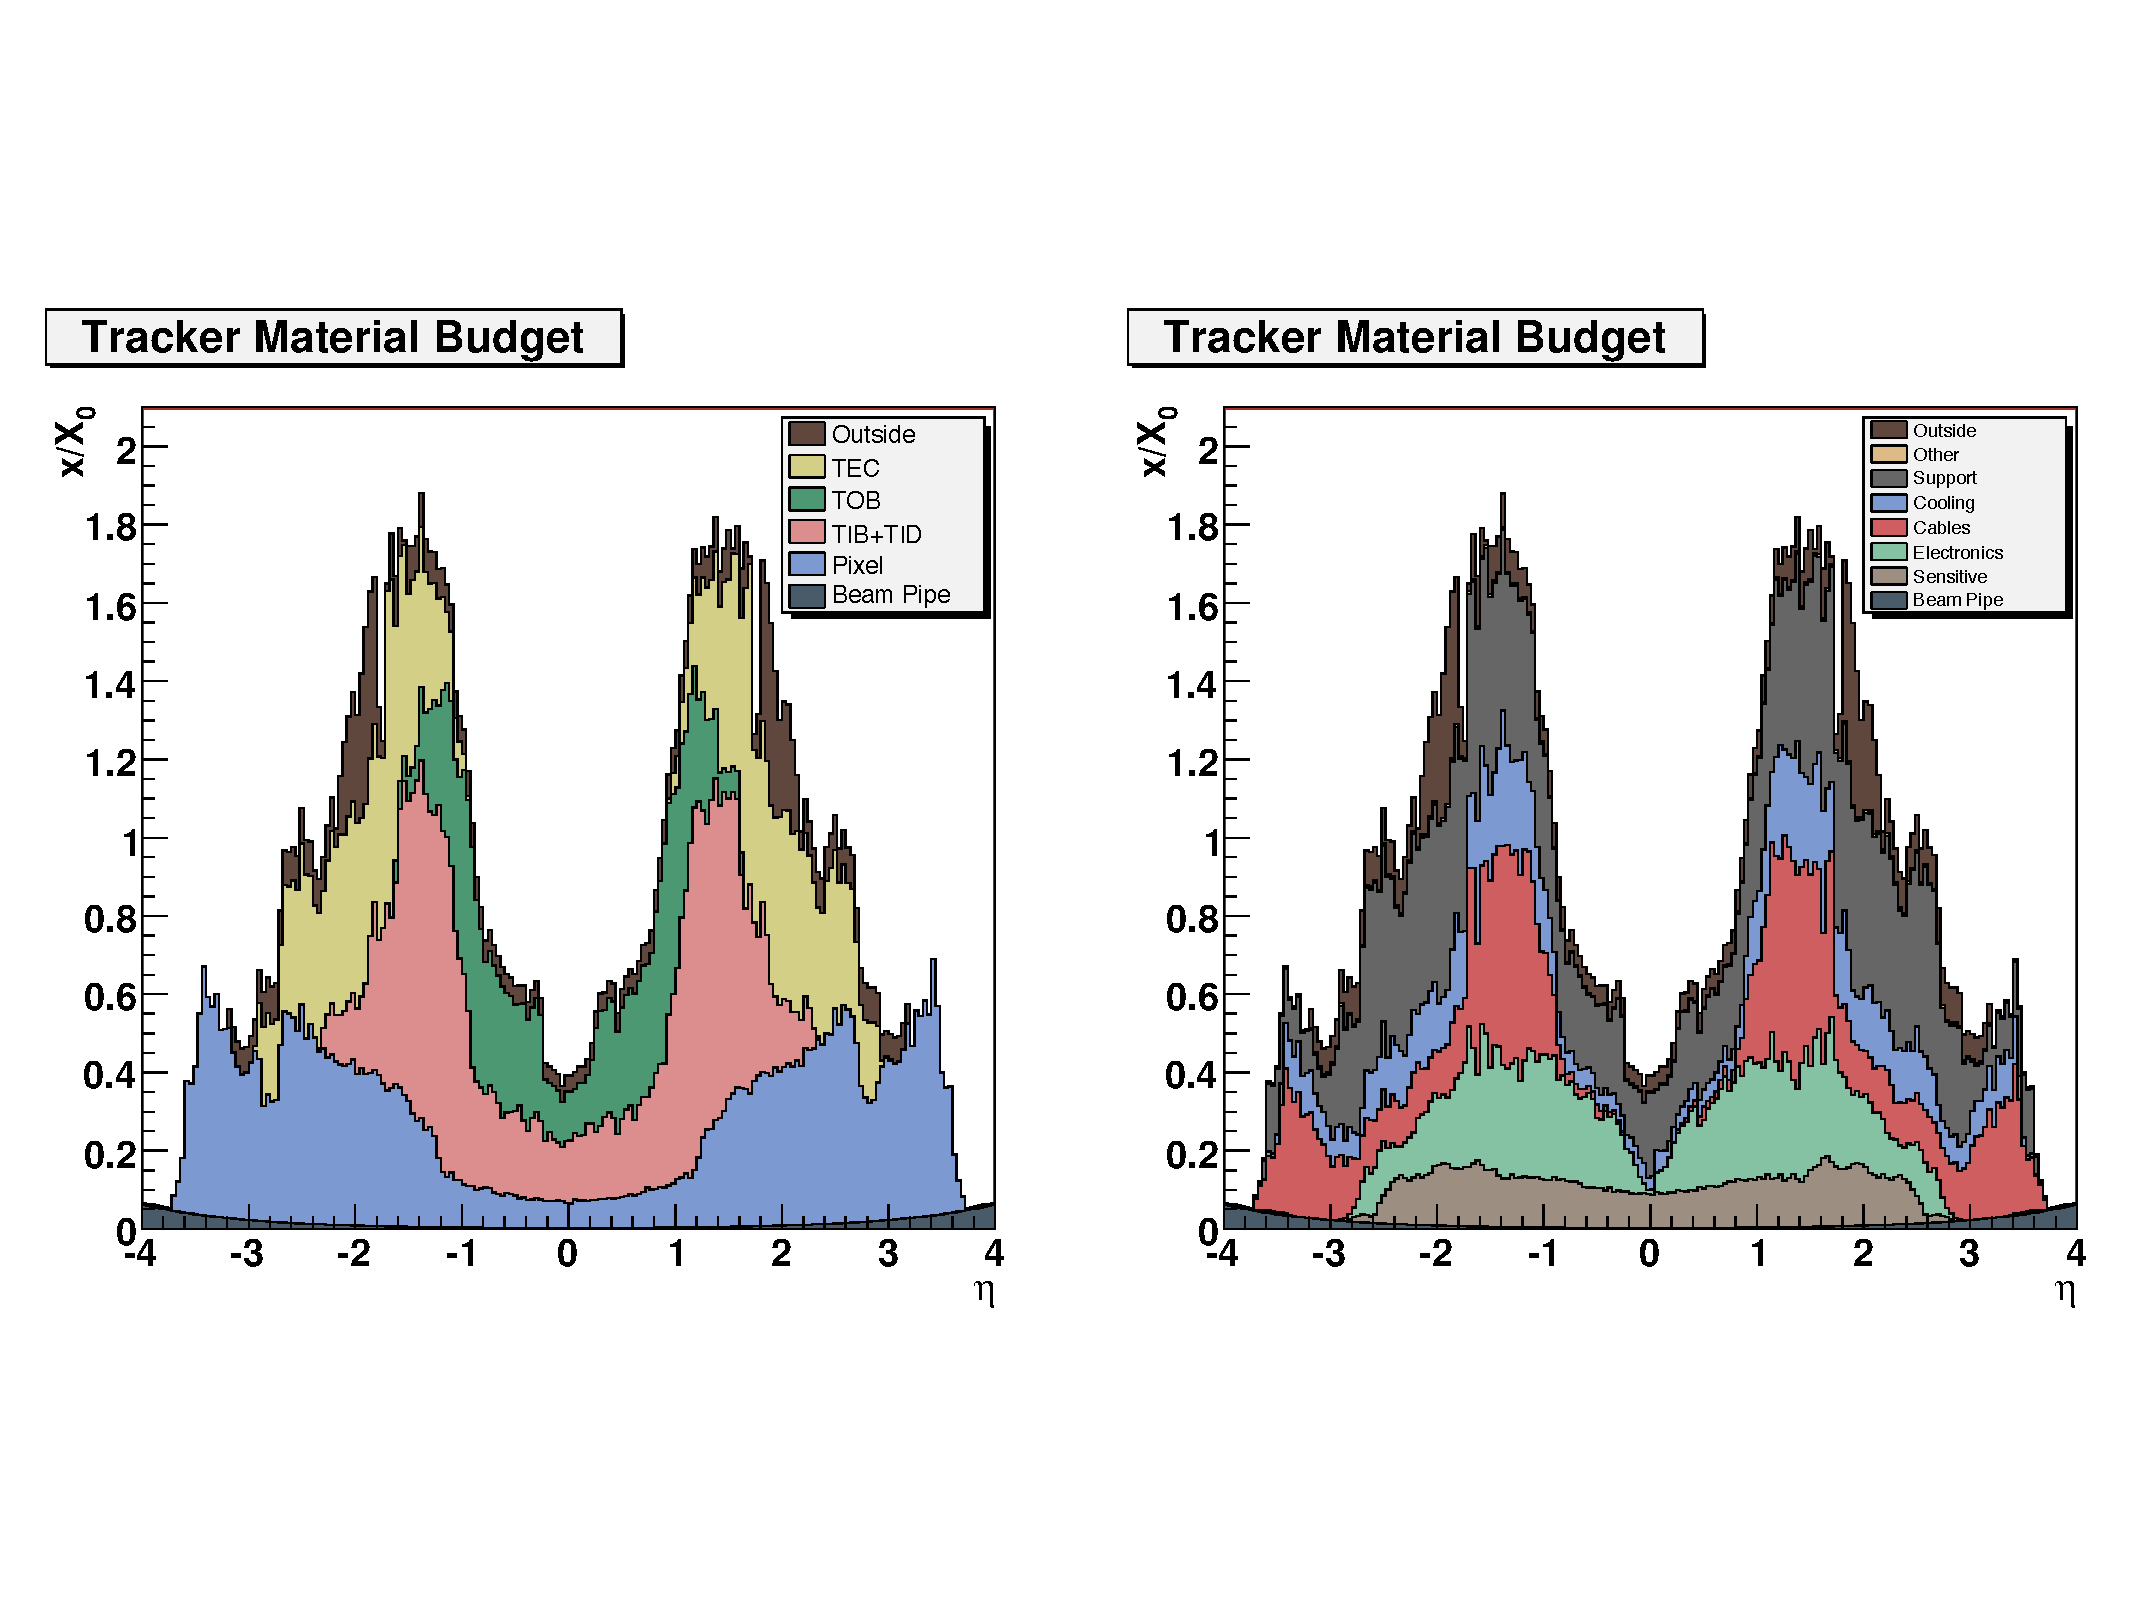
\includegraphics[width=0.99\textwidth]{CMS_DetectorFigures/TrackerMaterialBudget.pdf}
 \caption{Material budget of the CMS tracker in units of radiation
   length as a function of pseudorapidity $\eta$ for the (left)
   different subdetectors and (right) functional contributions.\label{fig:materialBudget}}
\end{figure}
\subsection{Pixel Tracker}
The inner pixel detector is composed of three 53-cm-long cylindrical layers at a
radii of 4.4, 7.3, and 10.2 cm -- which is called BPix. It is finalized by two disks of pixel
modules at each side extending from approximately 6 to 15 cm in
radius -- which is called FPix. The barrel is composed of 672 full and 96 half modules, a full (half)
module is composed of 16 (8) read-out chips equipped with 52$\times$80 pixels
of size 100$\times$150 $\mu$m. A completed full-module has the
dimensions of 66 mm$\times$26 mm and is provided with readout and
power. Figure~\ref{fig:Bpix} shows a completed full- and half- module as
well as an schematic of the different component integrated in the
module. The two disks at each side of the pixel barrel (see
Figure~\ref{fig:trackerlayout}) is composed 24 modules -- with a
trapezoidal geometry. Each disk is composed of two different
panel types; the first and closest to the interaction point is formed
by a 1$\times$2, 2$\times$3, 2$\times$4, and 1$\times$5 plaquettes
amounting to a total of 21 read-out chips; the second and furthest from
the interaction point is formed by a 2$\times$3, 2$\times$4, and 2$\times$5 plaquettes
amounting to a total of 24 read-out chips. A plaquette is the basic
unit of the FPix and consist of a single pixel sensor bump-bonded to
the read-out chip and wired-bonded to a very-high-density-interconnect
(VHDI) that provides data connections, power, and
control. Figure~\ref{fig:Fpix} show an schematic of these two
different panels as well as a photograph of a finalized
panel. Finally, a layout of the pixel traker system is given in
Figure~\ref{fig:PixelLayout} as well as the a detection efficiency as
a function of the pseudorapidity. The total number of pixels in the
pixel tracker is about 66 millions and they are equivalent to an area
of about 1 m$^2$.
\begin{figure}
 \centering
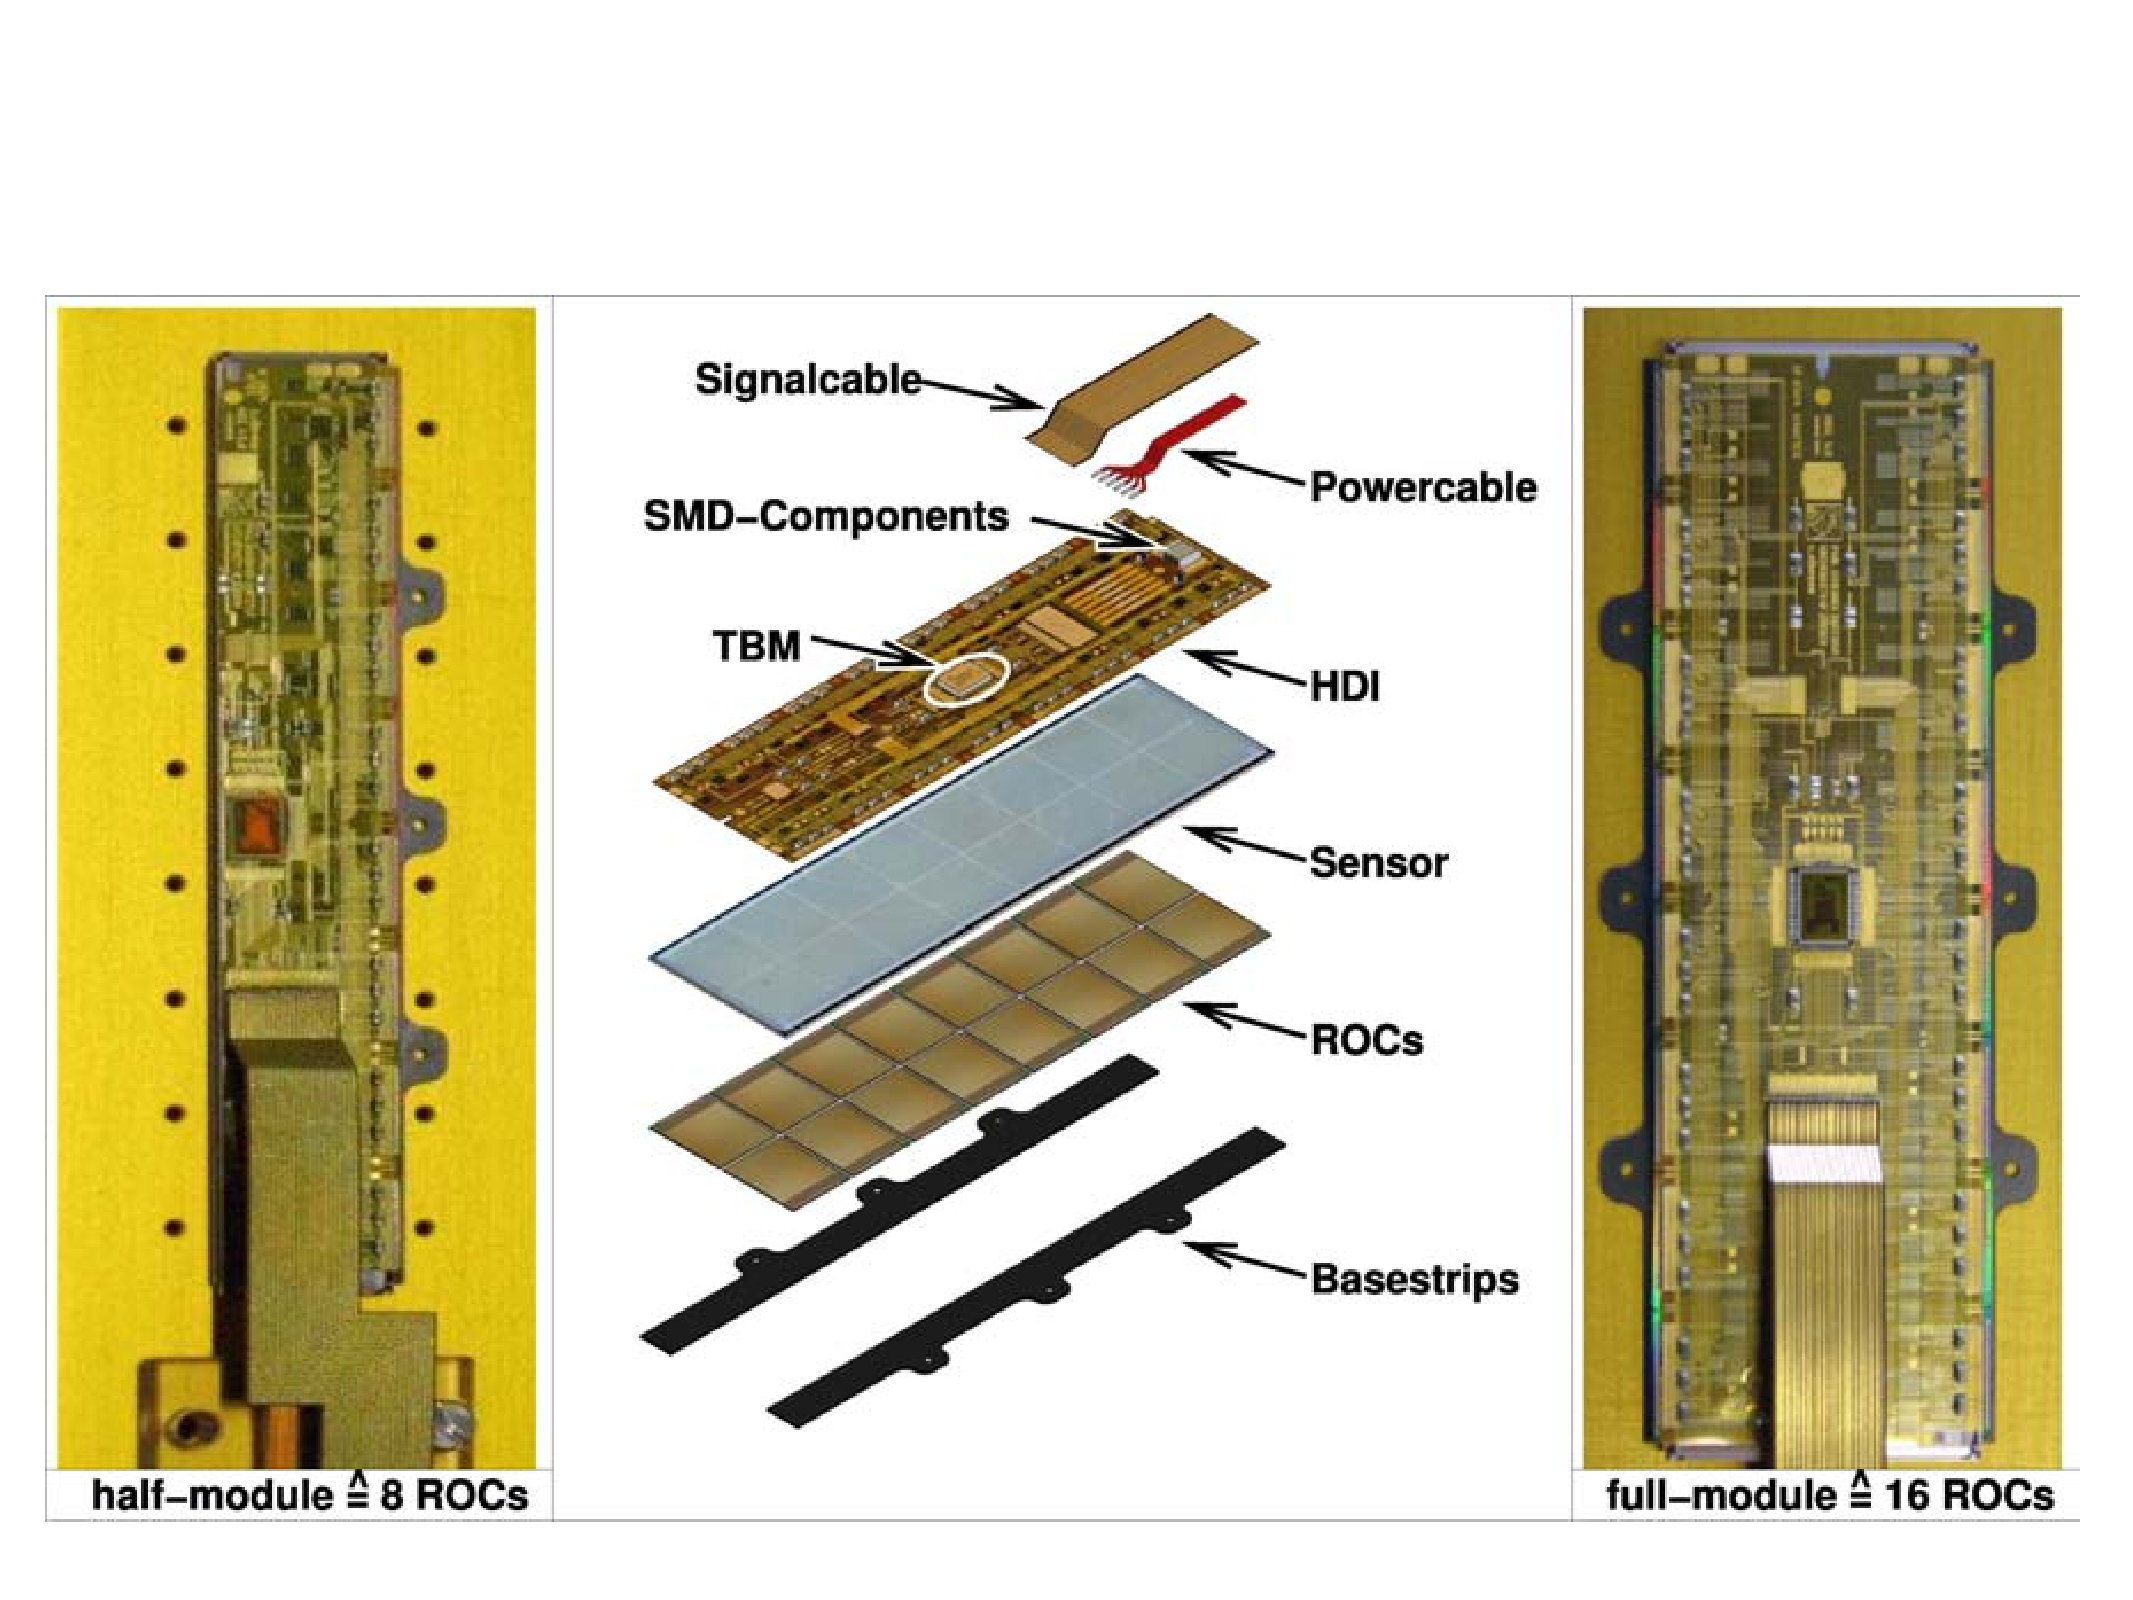
\includegraphics[width=0.99\textwidth]{CMS_DetectorFigures/BPixModule.pdf}
 \caption{BPix completed modules; (left) half-module, (center) an
   schematic of the different component forming the a full-module,(right) full-module.\label{fig:Bpix}}
\end{figure}
\begin{figure}
 \centering
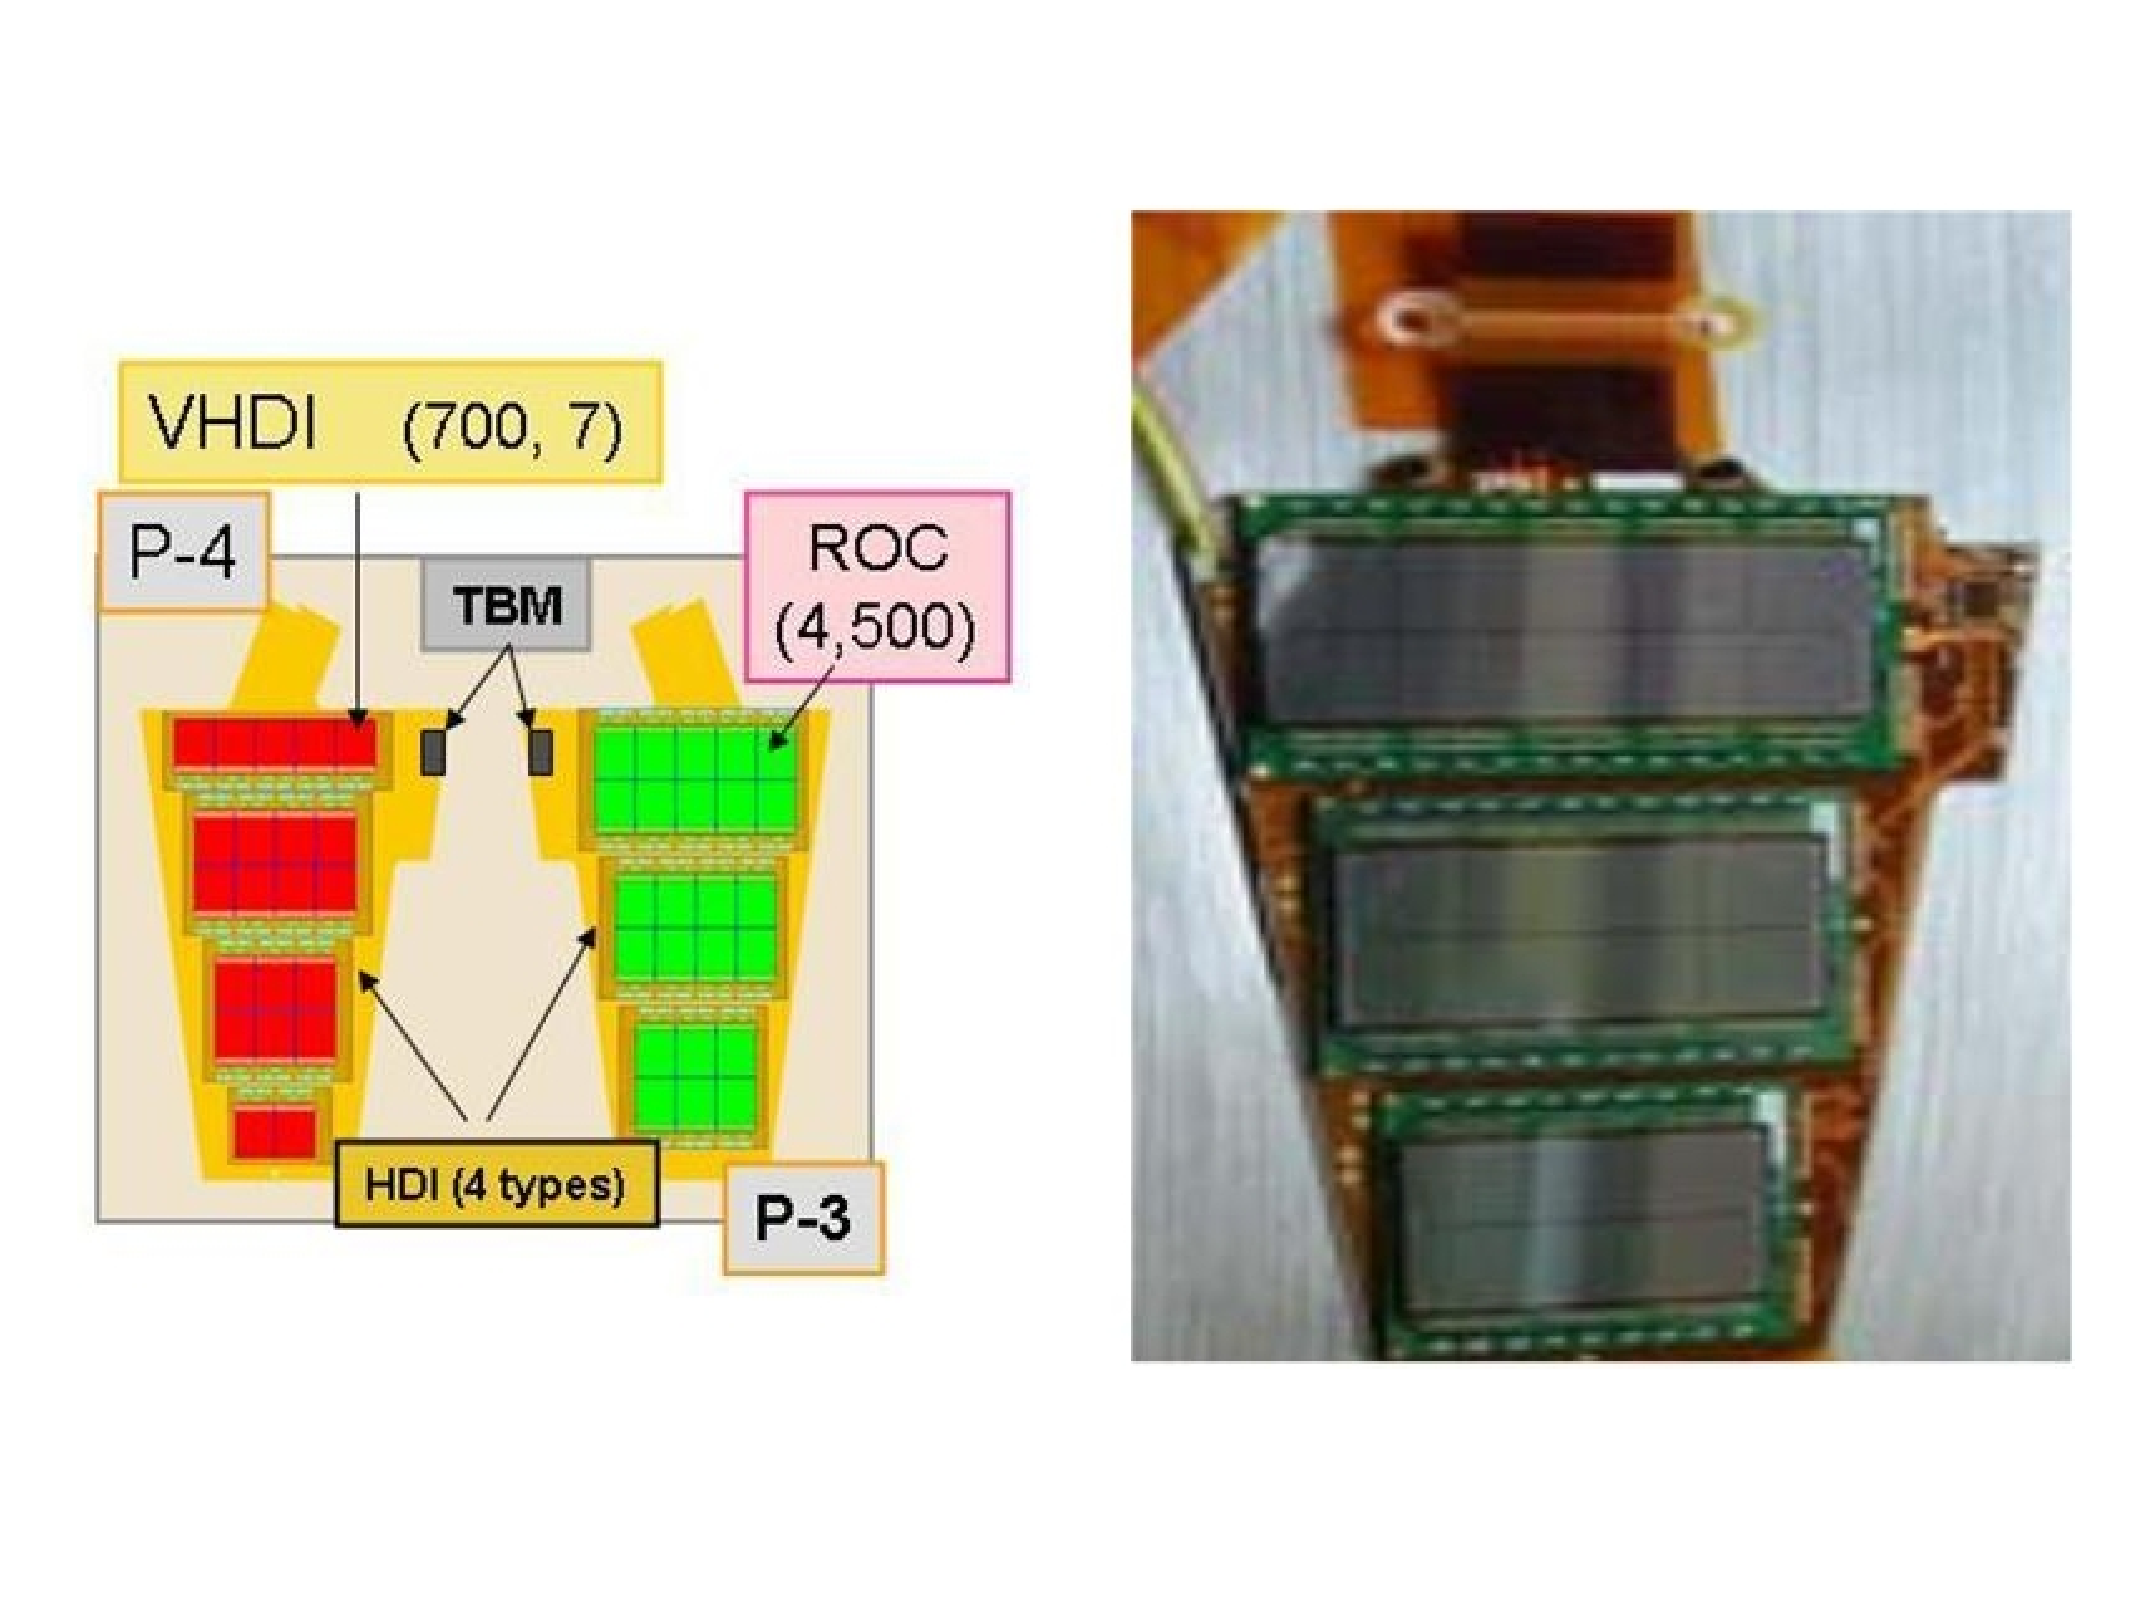
\includegraphics[width=0.99\textwidth]{CMS_DetectorFigures/FPixModule.pdf}
 \caption{FPix module; (left) an schematic of the two types of module,
   (right) a photograph of one of the completed FPix modules.\label{fig:Fpix}}
\end{figure}

\begin{figure}
 \centering
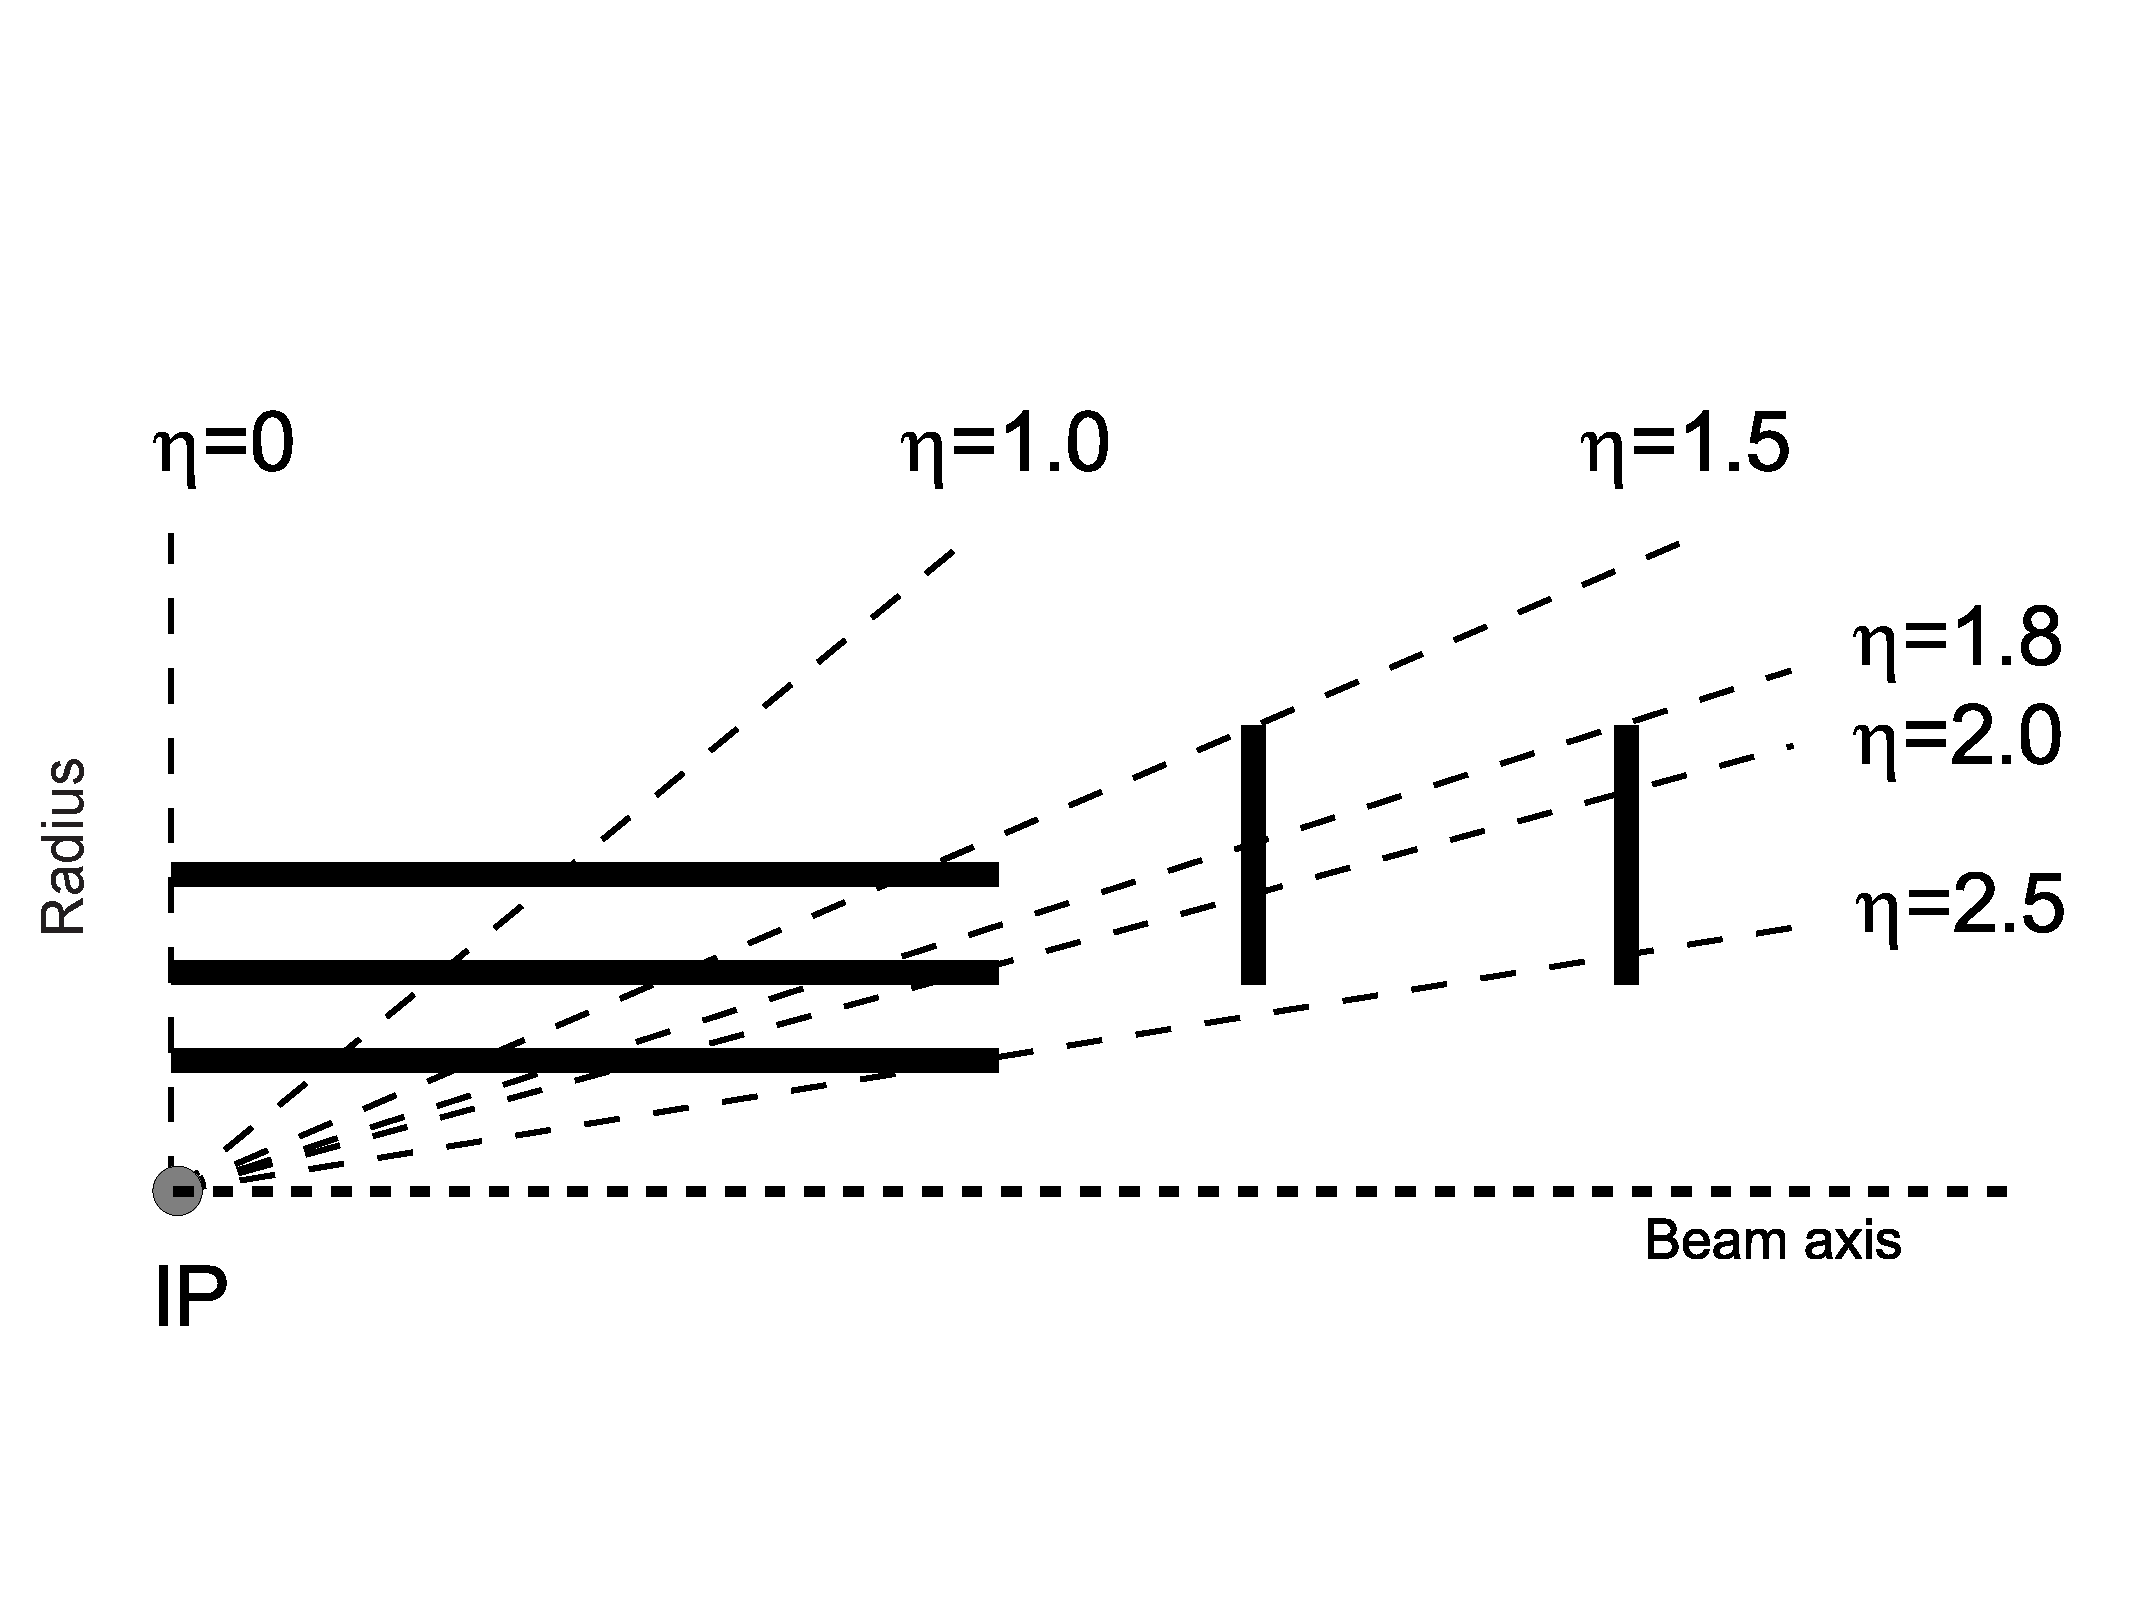
\includegraphics[width=0.49\textwidth]{CMS_DetectorFigures/PixelLayout.pdf}
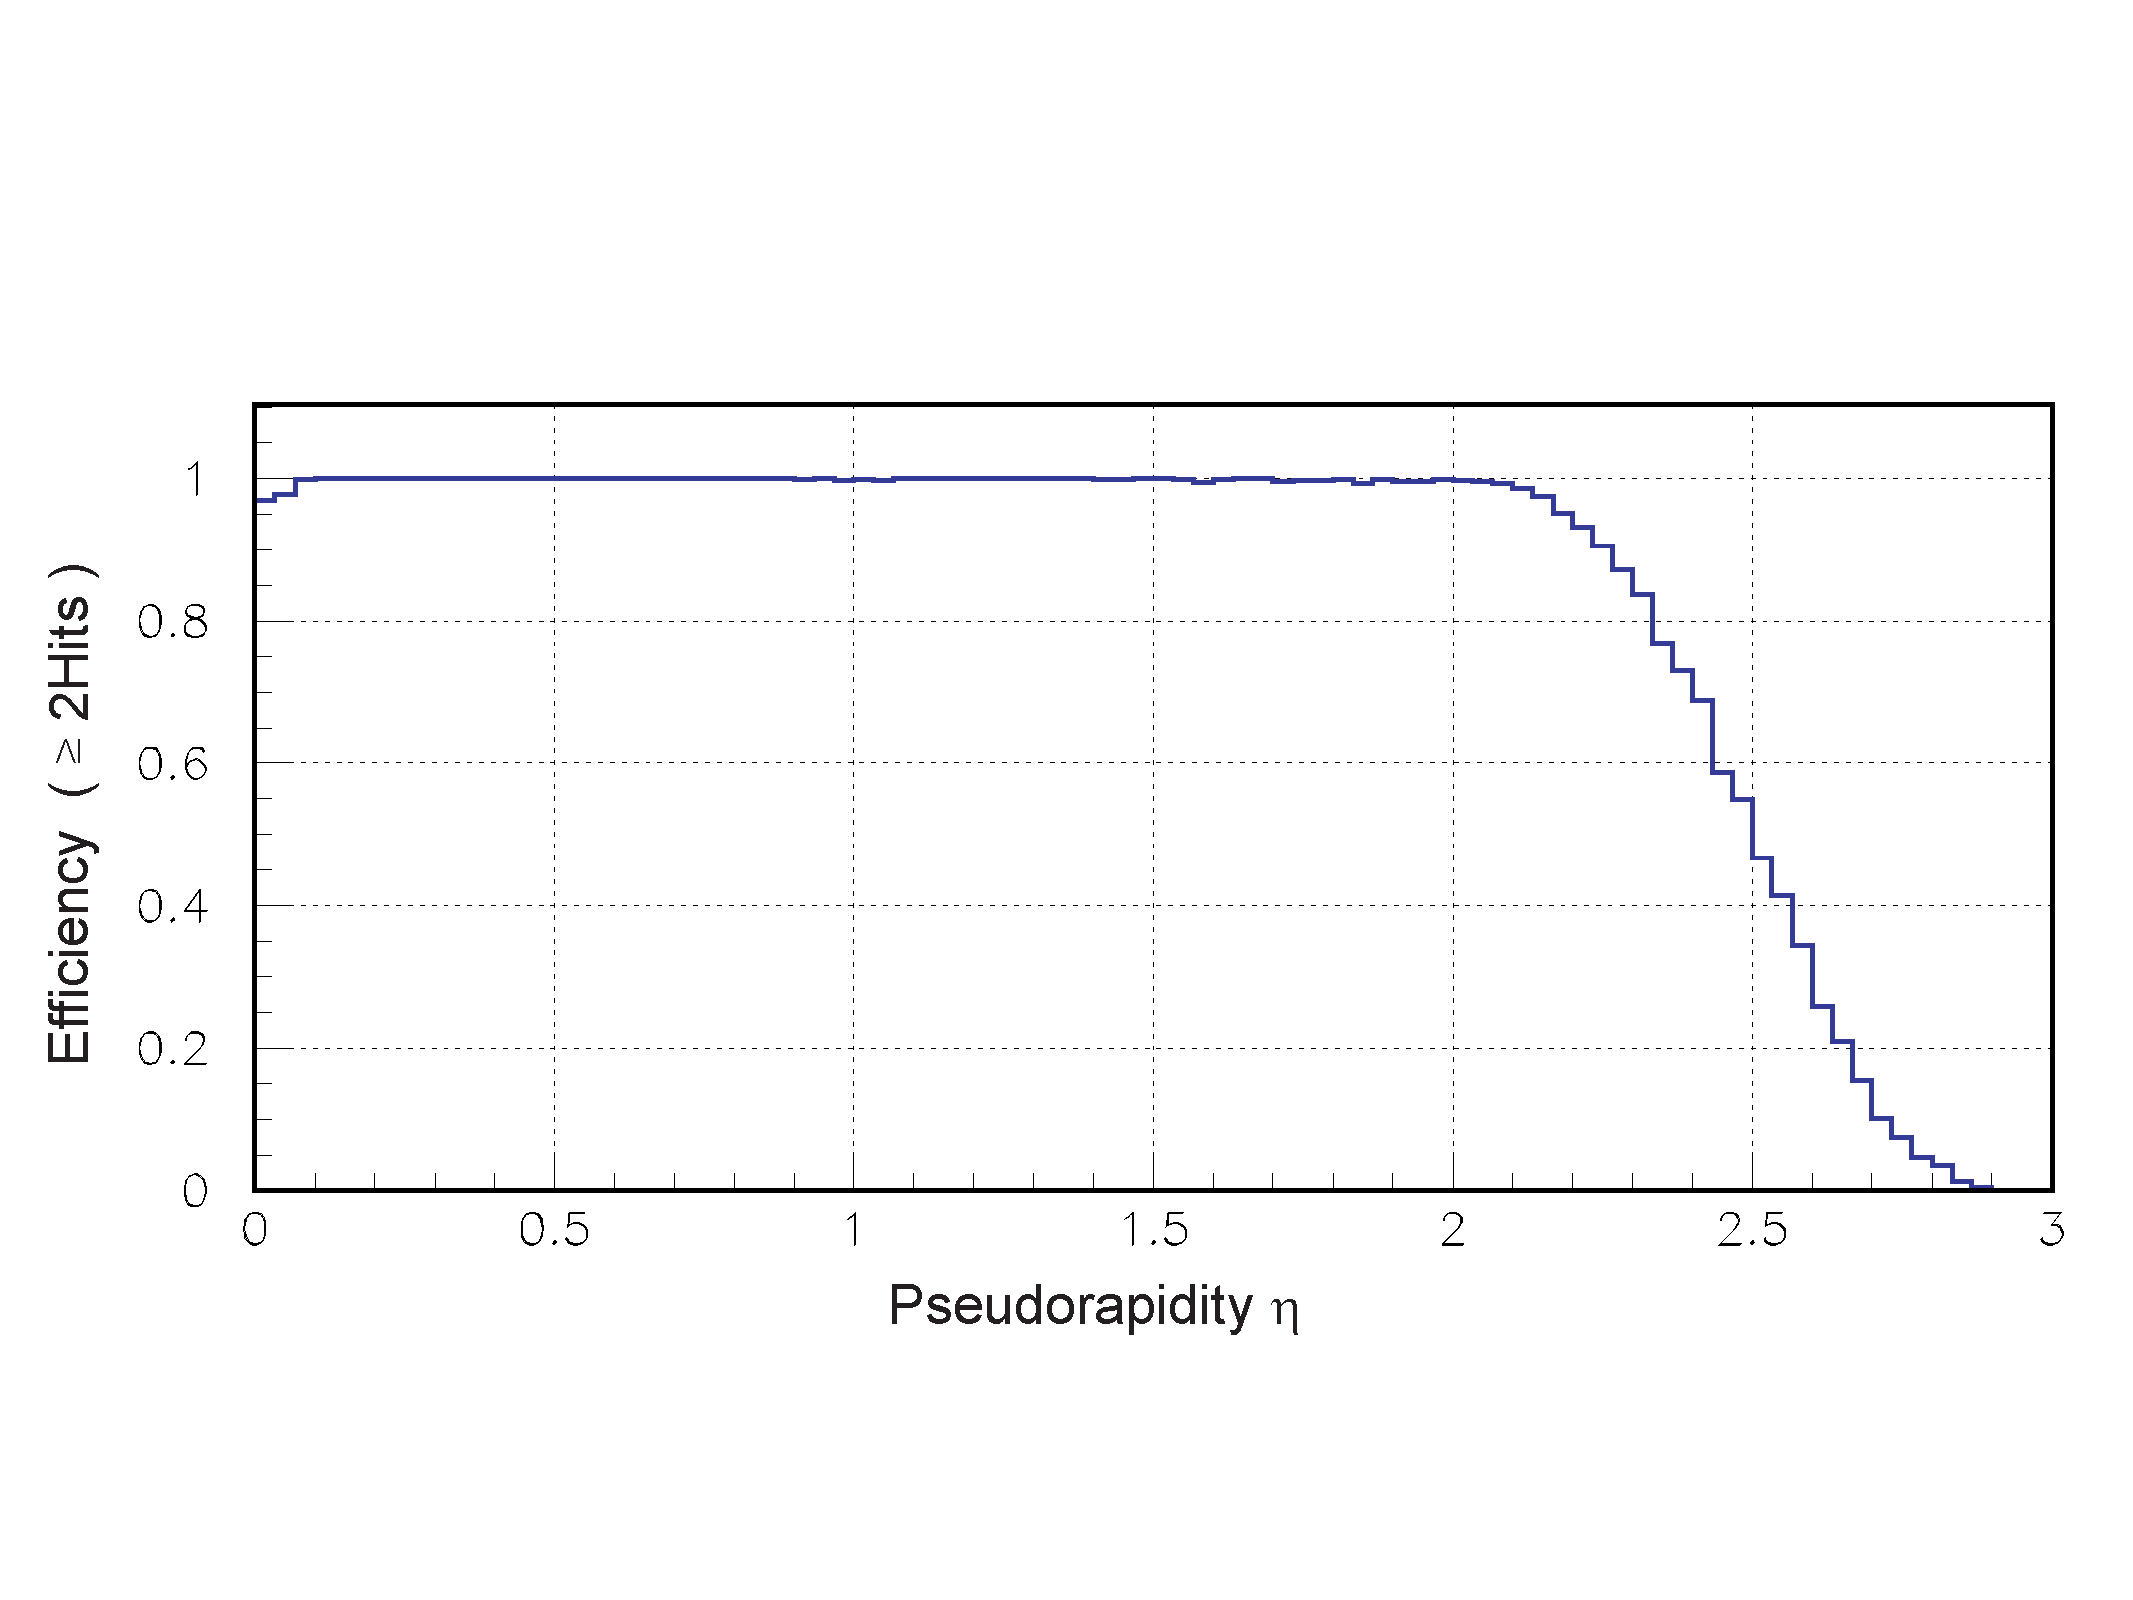
\includegraphics[width=0.49\textwidth]{CMS_DetectorFigures/PixelEfficiency.pdf}
 \caption{(Left) the layput of the silicon pixel tracker, (right) the
   pixel tracker detection efficiency as a function of the pseudorapidity.\label{fig:PixelLayout}}
\end{figure}
\subsection{Strip Tracker}
The silicon tracker is located outside the inner pixel tracker and is
composed of three subsystems that extend from 20 cm to 116 cm in the
radial direction. The Tracker Inner Barrel and Disks (TIB/TID) are
the innermost subsystem extending up to a radius of 55 cm, it includes
4 barrel layers and 3 disks at each side. The TIB/TID with their 320
$\mu$m thick silicon micro-strip sensor oriented along the $z$-axis records up to 4 $r$-$\phi$
measurements on a particle's trajectory. The strips pitch  in the TIB -- the
distance between each strip -- varies between 80 $\mu$m and 120 $\mu$m
in layers 1-2 and 3-4, respectively. The resulting single point
resolution is therefore 23 $\mu$m and 35 $\mu$m for the 1-2 and 3-4
layers, respectively. The TID has strip pitches between 100 -140$\mu$m
-- resulting in single point resolution between 29-41 $\mu$m. The
TIB/TID is completely sorrounded by the Tracker Outer Barrel (TOB)
which with its 6 barrel layer extends up to a radious of 116 cm. The
layers are composed of 500 $\mu$m thick micro-strips sensor with
pitches of 183 $\mu$m and 122 $\mu$m for the firts 4  and last 2
layer, respectively -- recording up to 6 $r$-$\phi$
measurements on a particle's trajectory with single point resolutions of 53 $\mu$m
and $\mu$m, respectively. The TIB/TID and the TOB cover the region
with $|z|< 113$ cm, beyond this point (see
Figure~\ref{fig:trackerlayout}) the Tracker EndCaps (TEC$^{\pm}$) --
where the sign, obiously, represents the position on the $z$-axis --
extend from 124 cm $|z|< 282$ cm and 22.5 cm $|r|< 113.5$ cm. The TEC
consists of 9 disks which contains up to 7 rings of silicon
micro-strips, the later are 320 $\mu$m and 500 $\mu$m thick in the
inner 4 and outer 3 rings, respectively.
Additionally, modules in the two innermost layers in the TIB and TOB,
the two inner most rings of the TID, as well as rings 1,2 and 5 of the TECs are
equipped with a second micro-strip detector module that is mounted
back-to-back allowing measurements on the perpedicular coordinate --
i.e. $z$ and r in the barrel and the disks, respectively. In this
fashion at least $\approx$ 9 hits in the silicon strip tracker in the
$|\eta|<2.4$ range are ensure, with at least $\approx$ 4
two-dimensional measurements. The full strip tracker amounts to a
total of 9.3 million strips and covers an active are of silicon equal
to 198 m$^2$.

\subsection{Performance of the CMS Tracker}

The tracker efficiency for single muons is measured in 7\TeV data as a
function of the muon pseudorapidity $\eta$ and the number of
reconstructed vertices using the tag-and-probe technique on muons
decaying from Z bosons. The results are shown in
Figure~\ref{fig:MuonEfficiency}, where the muon efficiency is above
99\% within the tracker acceptance and up to 20 reconstructed
vertices. The muon transverse momentum and transverse impact
paramenter resolution as a function of  $\eta$ are estimated from the
CMS full simulation, the results are shown in left and right panel of
Figure~\ref{fig:MuonResolution}, respectively. The muon transverse
momentum resolution is about 1-3\% for $|\eta|<1.5$ for muons of
different energies. The transverse impact parameter is estimated to be
between $\sim$10-20 $\mu$m for a 100\GeV muon while the for 1\GeV muons the
resolution is between $\sim$ 80-250 $\mu$m.

\begin{figure}
 \centering
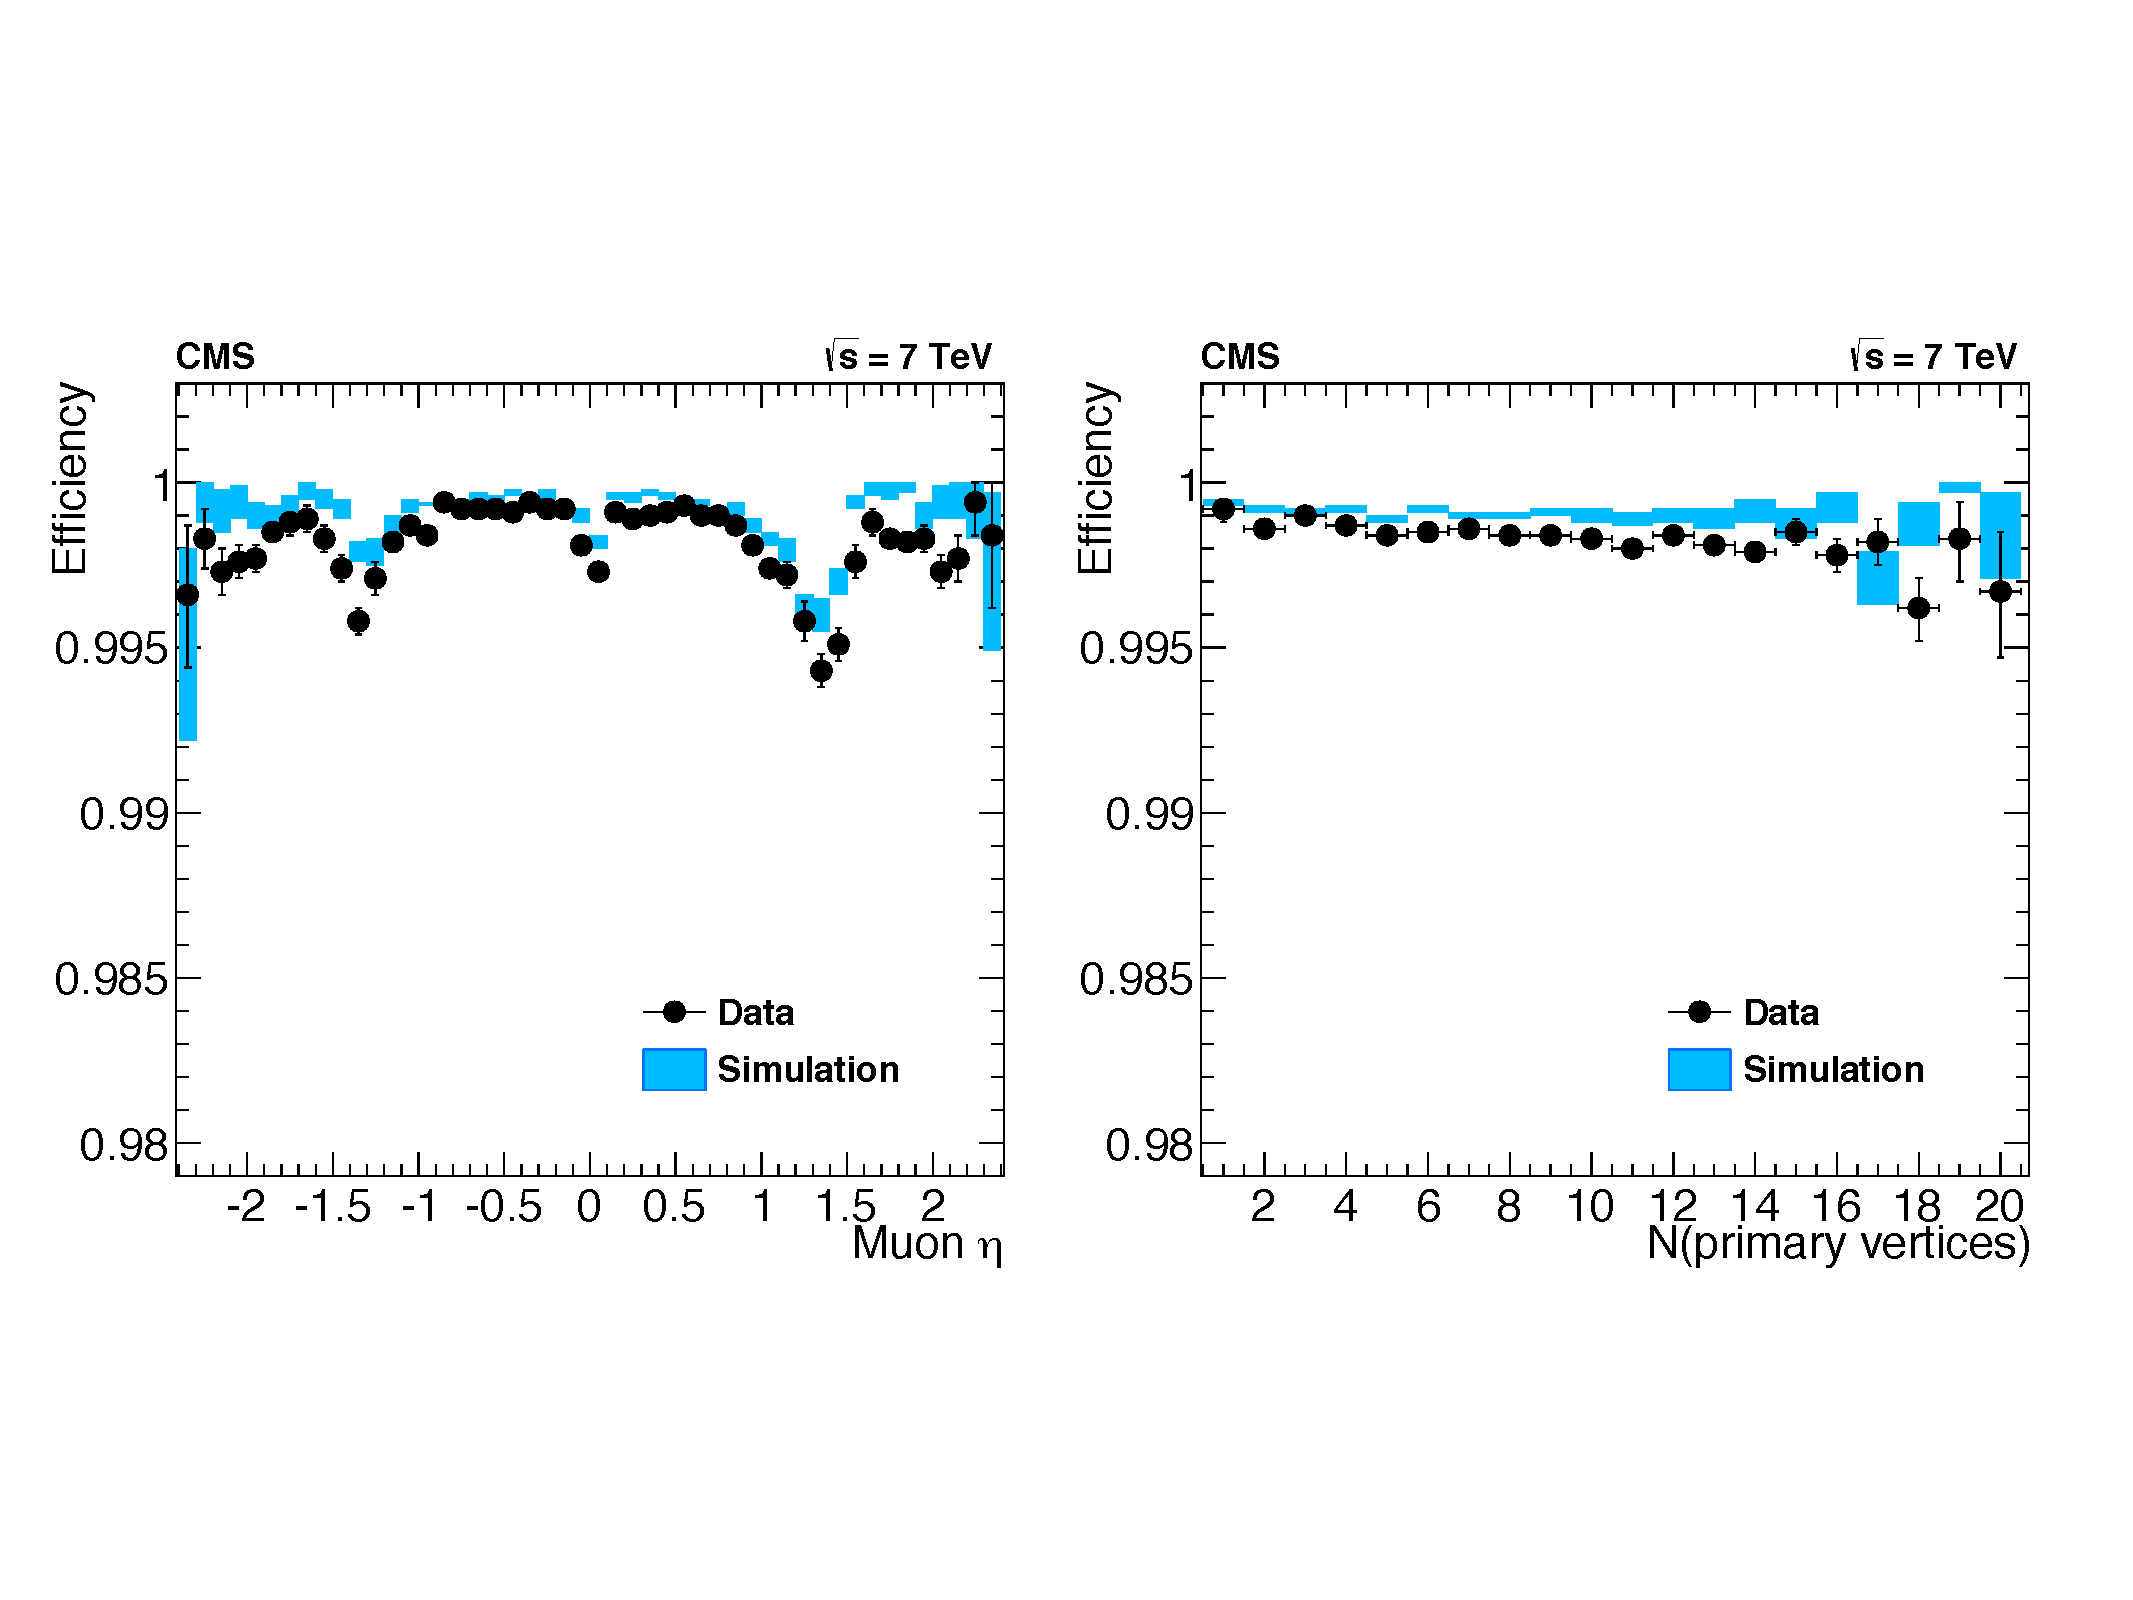
\includegraphics[width=0.99\textwidth]{CMS_DetectorFigures/TrackerMuonEff.pdf}
\caption{Tracking efficiency for muons from Z decays using the tag-and
 -probe technique. The left panel and right panel show the efficiency
 as function of the muon $\eta$ and the number of reconstructed
 vertices, respectively. The black dots represent the measurement in
 7\TeV data and the solid color represents the CMS simulation.\label{fig:MuonEfficiency}}
\end{figure}

\begin{figure}
 \centering
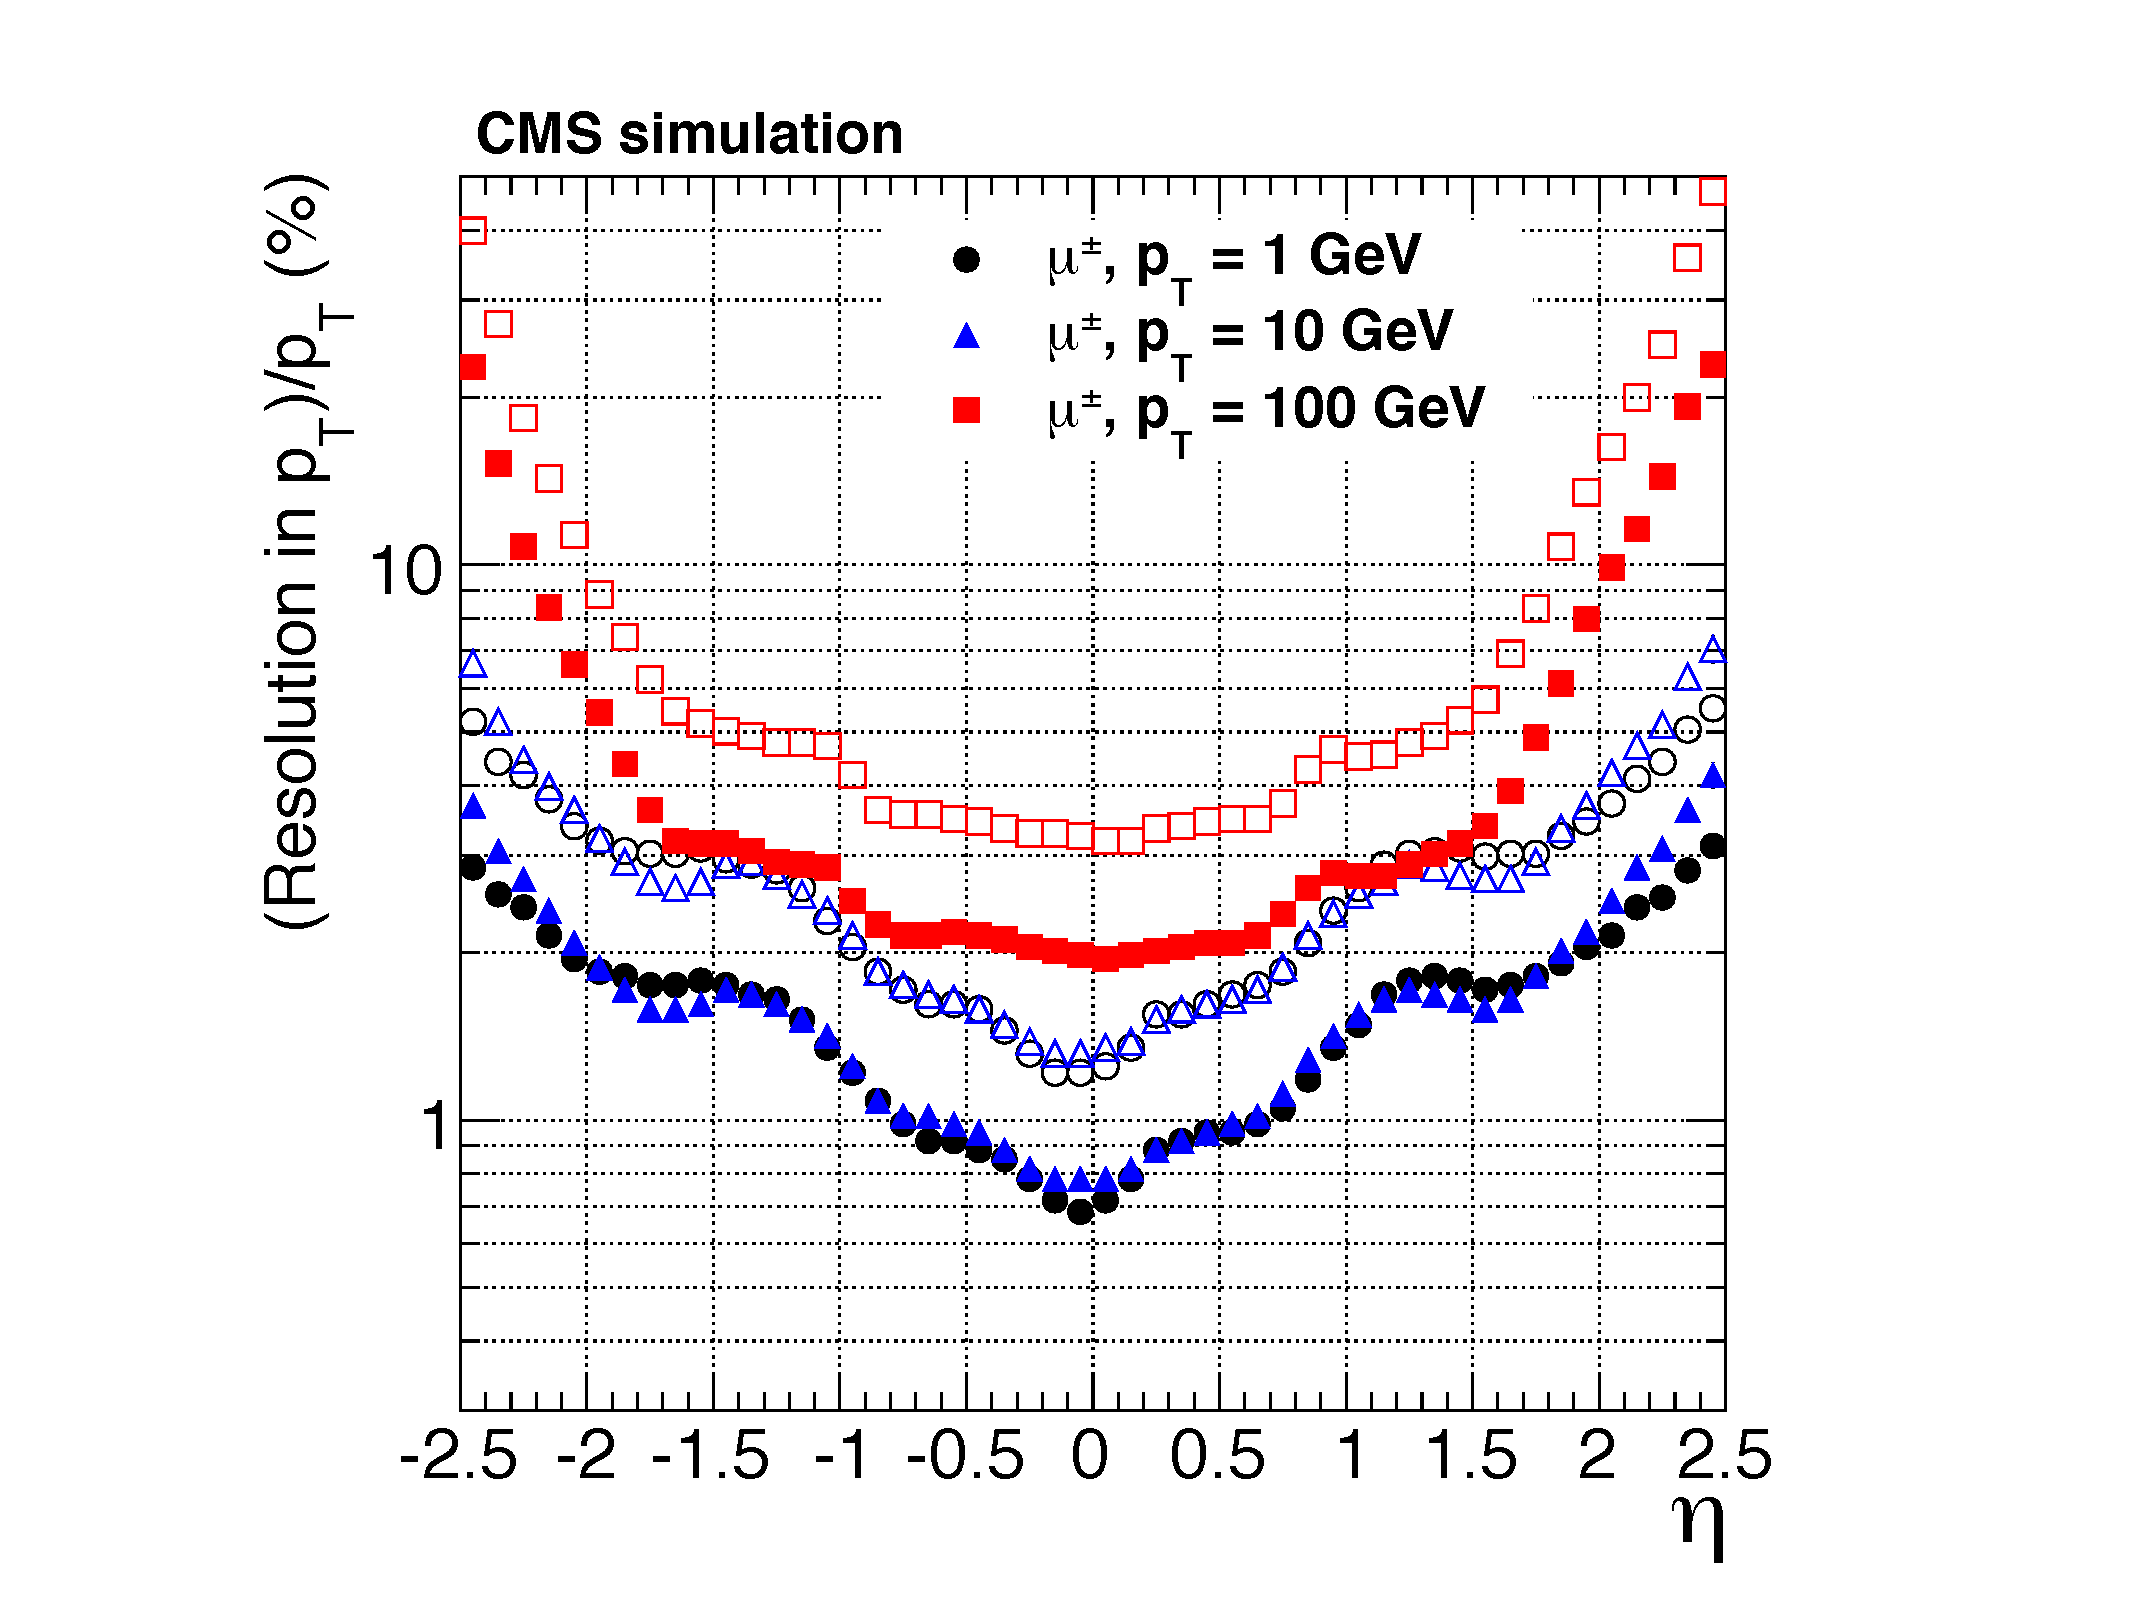
\includegraphics[width=0.49\textwidth]{CMS_DetectorFigures/TrackerPtResolution.pdf}
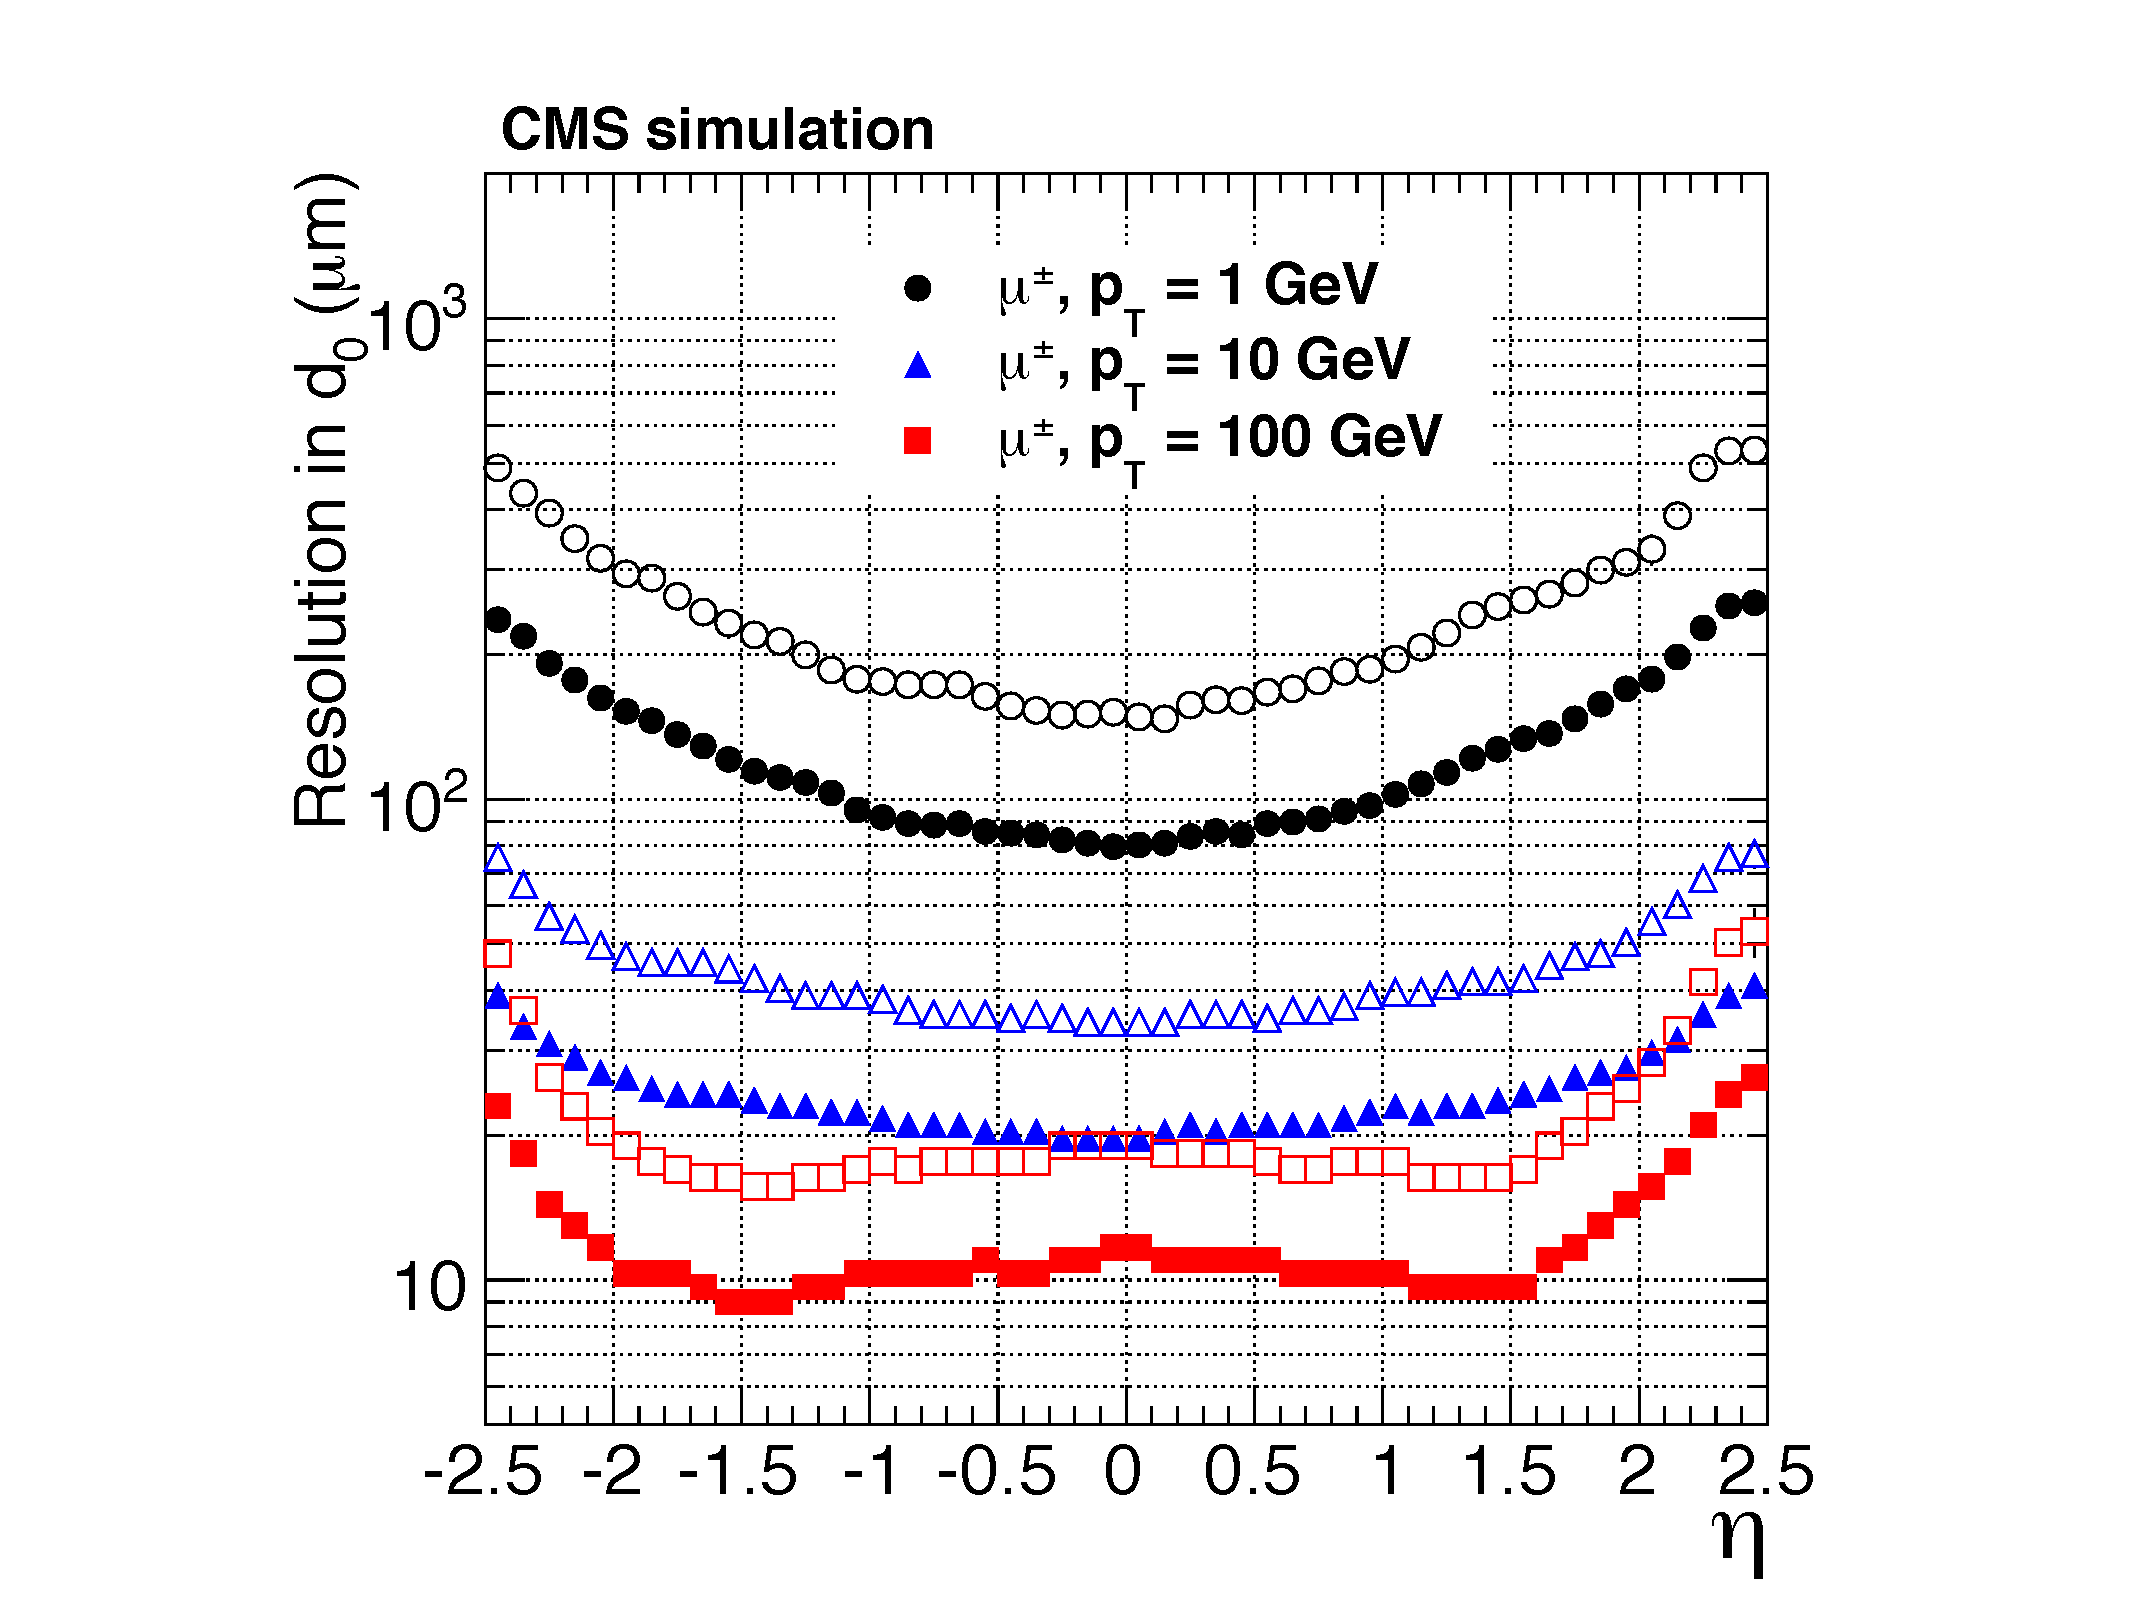
\includegraphics[width=0.49\textwidth]{CMS_DetectorFigures/TrackerImpactParameterResolution.pdf}
 \caption{Resolution as a function of the pseudorapidity $\eta$ for
   muons of $p_{\mathrm{T}} = $ 1, 10, and 100\GeV. The left panel
   shows the trasverse momentum resolution and the right panel the
   transverse impact parameter resolution. Both quantities are
   estimated from Simulation.\label{fig:MuonResolution}}
\end{figure}



\section{The Electromagnetic Calorimeter}
The CMS electromagnectic calorimeter (ECAL) is a granular and homogeneous
calorimeted built out of 61,200 lead tungstate (PbWO$_{4}$) crystals
in the barrel and closed by 7,324 PbWO$_{4}$ crystals in each of the
two endcaps. Additionally, a preshower detector is place in front of
the endcaps -- i.e. closer to the interaction point. The scintillating
light is collected by silicon avalanche photodiodes (APDs) in the ECAL barrel
(EB) and by vacuum phototriodes (VPTs) in the ECAL endcaps
(EE). Figure~\ref{fig:ECALgeometry} shows a projectional schematic
layout as well as a geometric view of a quarter of the CMS ECAL. The
ECAL excellent performance is one of the keystones of the physics
results of the CMS experiment, perhaps, best exemplyfied by the Higgs
boson search and characterization in the H$\rightarrow\gamma\gamma$
and H$\rightarrow$ZZ$^{*}$ decay channels~\cite{CMSHgg, CMSHzz}.

\begin{figure}
 \centering
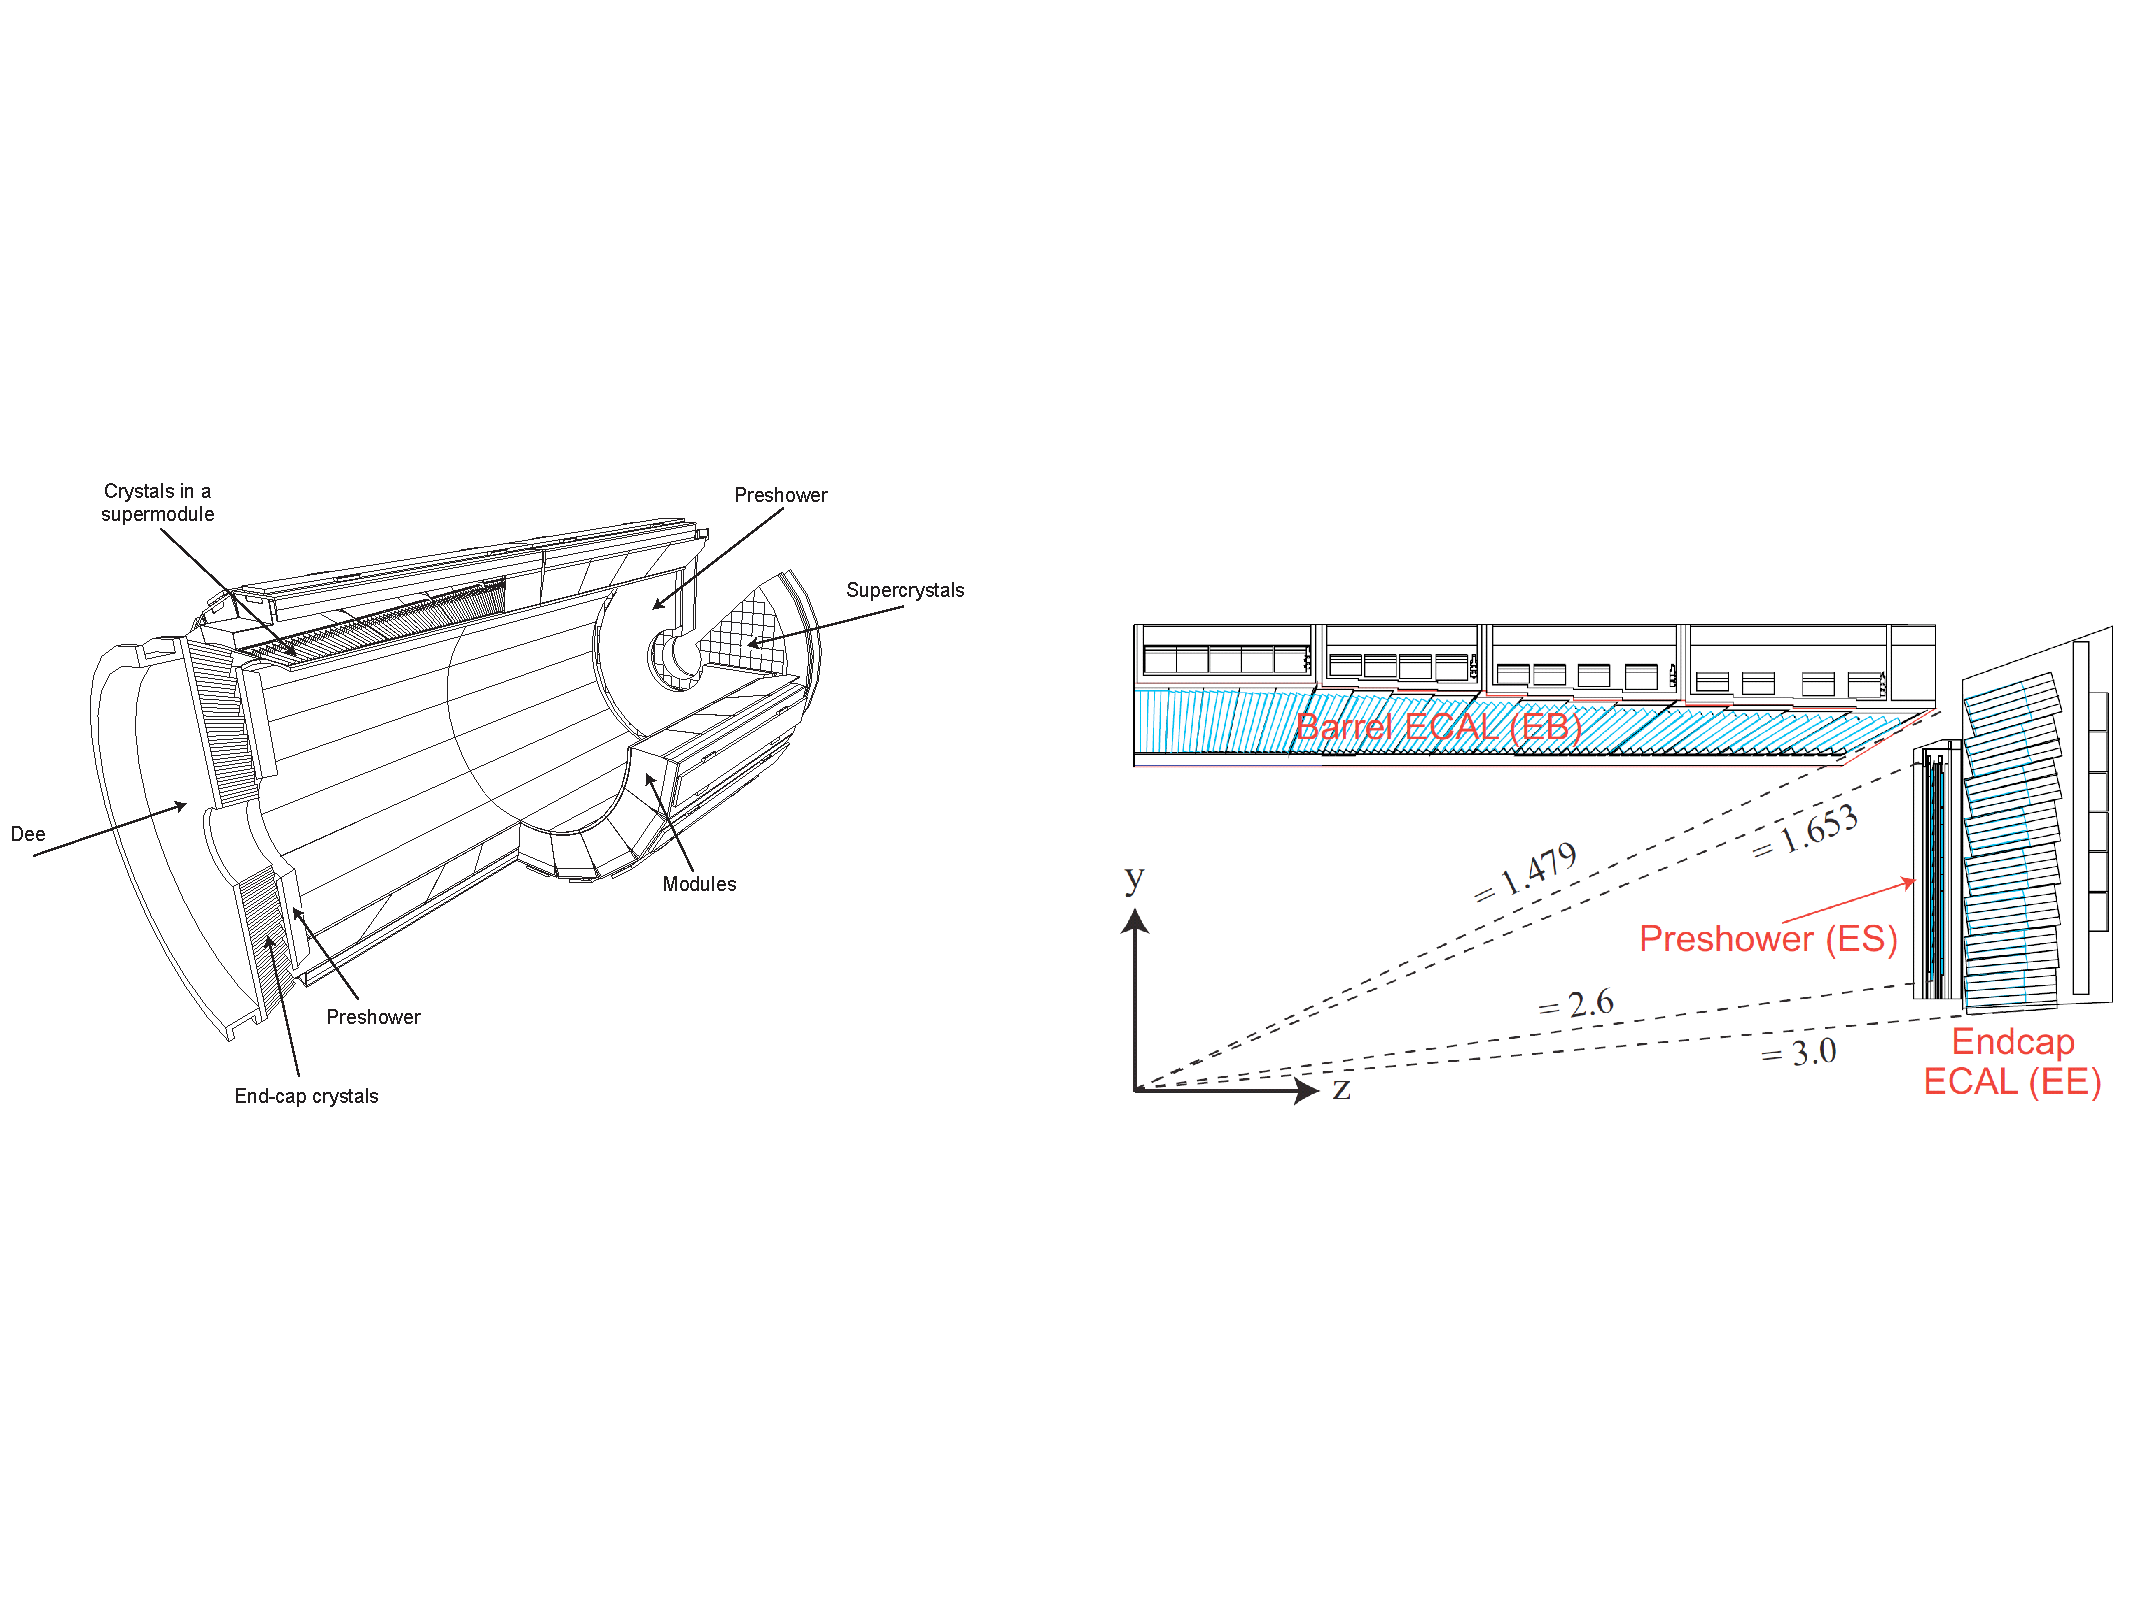
\includegraphics[width=0.99\textwidth]{CMS_DetectorFigures/ECAL_Geometry.pdf}
\caption{The layout of the CMS electromagnetic calorimenter. The left
  panel shows a projectional schematic
layout including all the major parts while the left panel shows a
geometric view of a quarter of the ECAL.\label{fig:ECALgeometry}}
\end{figure}

The PbWO$_{4}$ crystals with a density of 8.28 g/cm$^{3}$ provided a
good candidate because of its small radiation length ($X_{0} = 0.89$
cm), small moli\`ere radious (2.19 cm), and fast response. PbWO$_{4}$
crystals have a relatively low light yield of about 10
photo-electrons/MeV and therefore they required to be read out by
sensors with internal amplification inside the 3.8 T magnetic
field. The crystals in the EB are 23 cm long and have a
cross-sectional area of 2.2$\times$2.2 cm$^{2}$ (equivalent to
0.0174$\times$0.0174 in $\eta$, $\phi$), they are located at radious
of 1.29 m and arranged
in a quasi-projective geometry with 170 crystals -- 85 at each side --  covering up to a pseudorapidity range
$|\eta| < 1.48$. With 360 crytals in the $\phi$  direction the EB is
fully hermetic. The EE crystals are located at $z = \pm$ 315.4 cm, they
have a cross-sectional are of 2.86$\times$2.86 cm$^{2}$  and
3.0$\times$3.0 cm$^{2}$ at the front an rear faces, respectively, and
a length of 22 cm. They crystals are grouped in mechanical structure
of 5$\times$5 crystals and arranged in the traditional $x$-$y$
directions. Each endcap is divided into halves or \textit{Dees},
holding 3,662 crystals. The EE extends the ECAL coverage up to the
range $1.479 < |\eta| < 3.0$. The left and right panels of
Figure~\ref{fig:ECALcrystals} show the EB crystal instrumented with an
APD ant the EE crystal instrumented with a VPT, respectively.  Real
photographs of an EB module equipped with crystal is presented in
Figure~\ref{fig:ECALEB_module} while an EE Dee fully instrumented with crystals is shown
in Figure~\ref{fig:ECALEE_module}.
\begin{figure}
 \centering
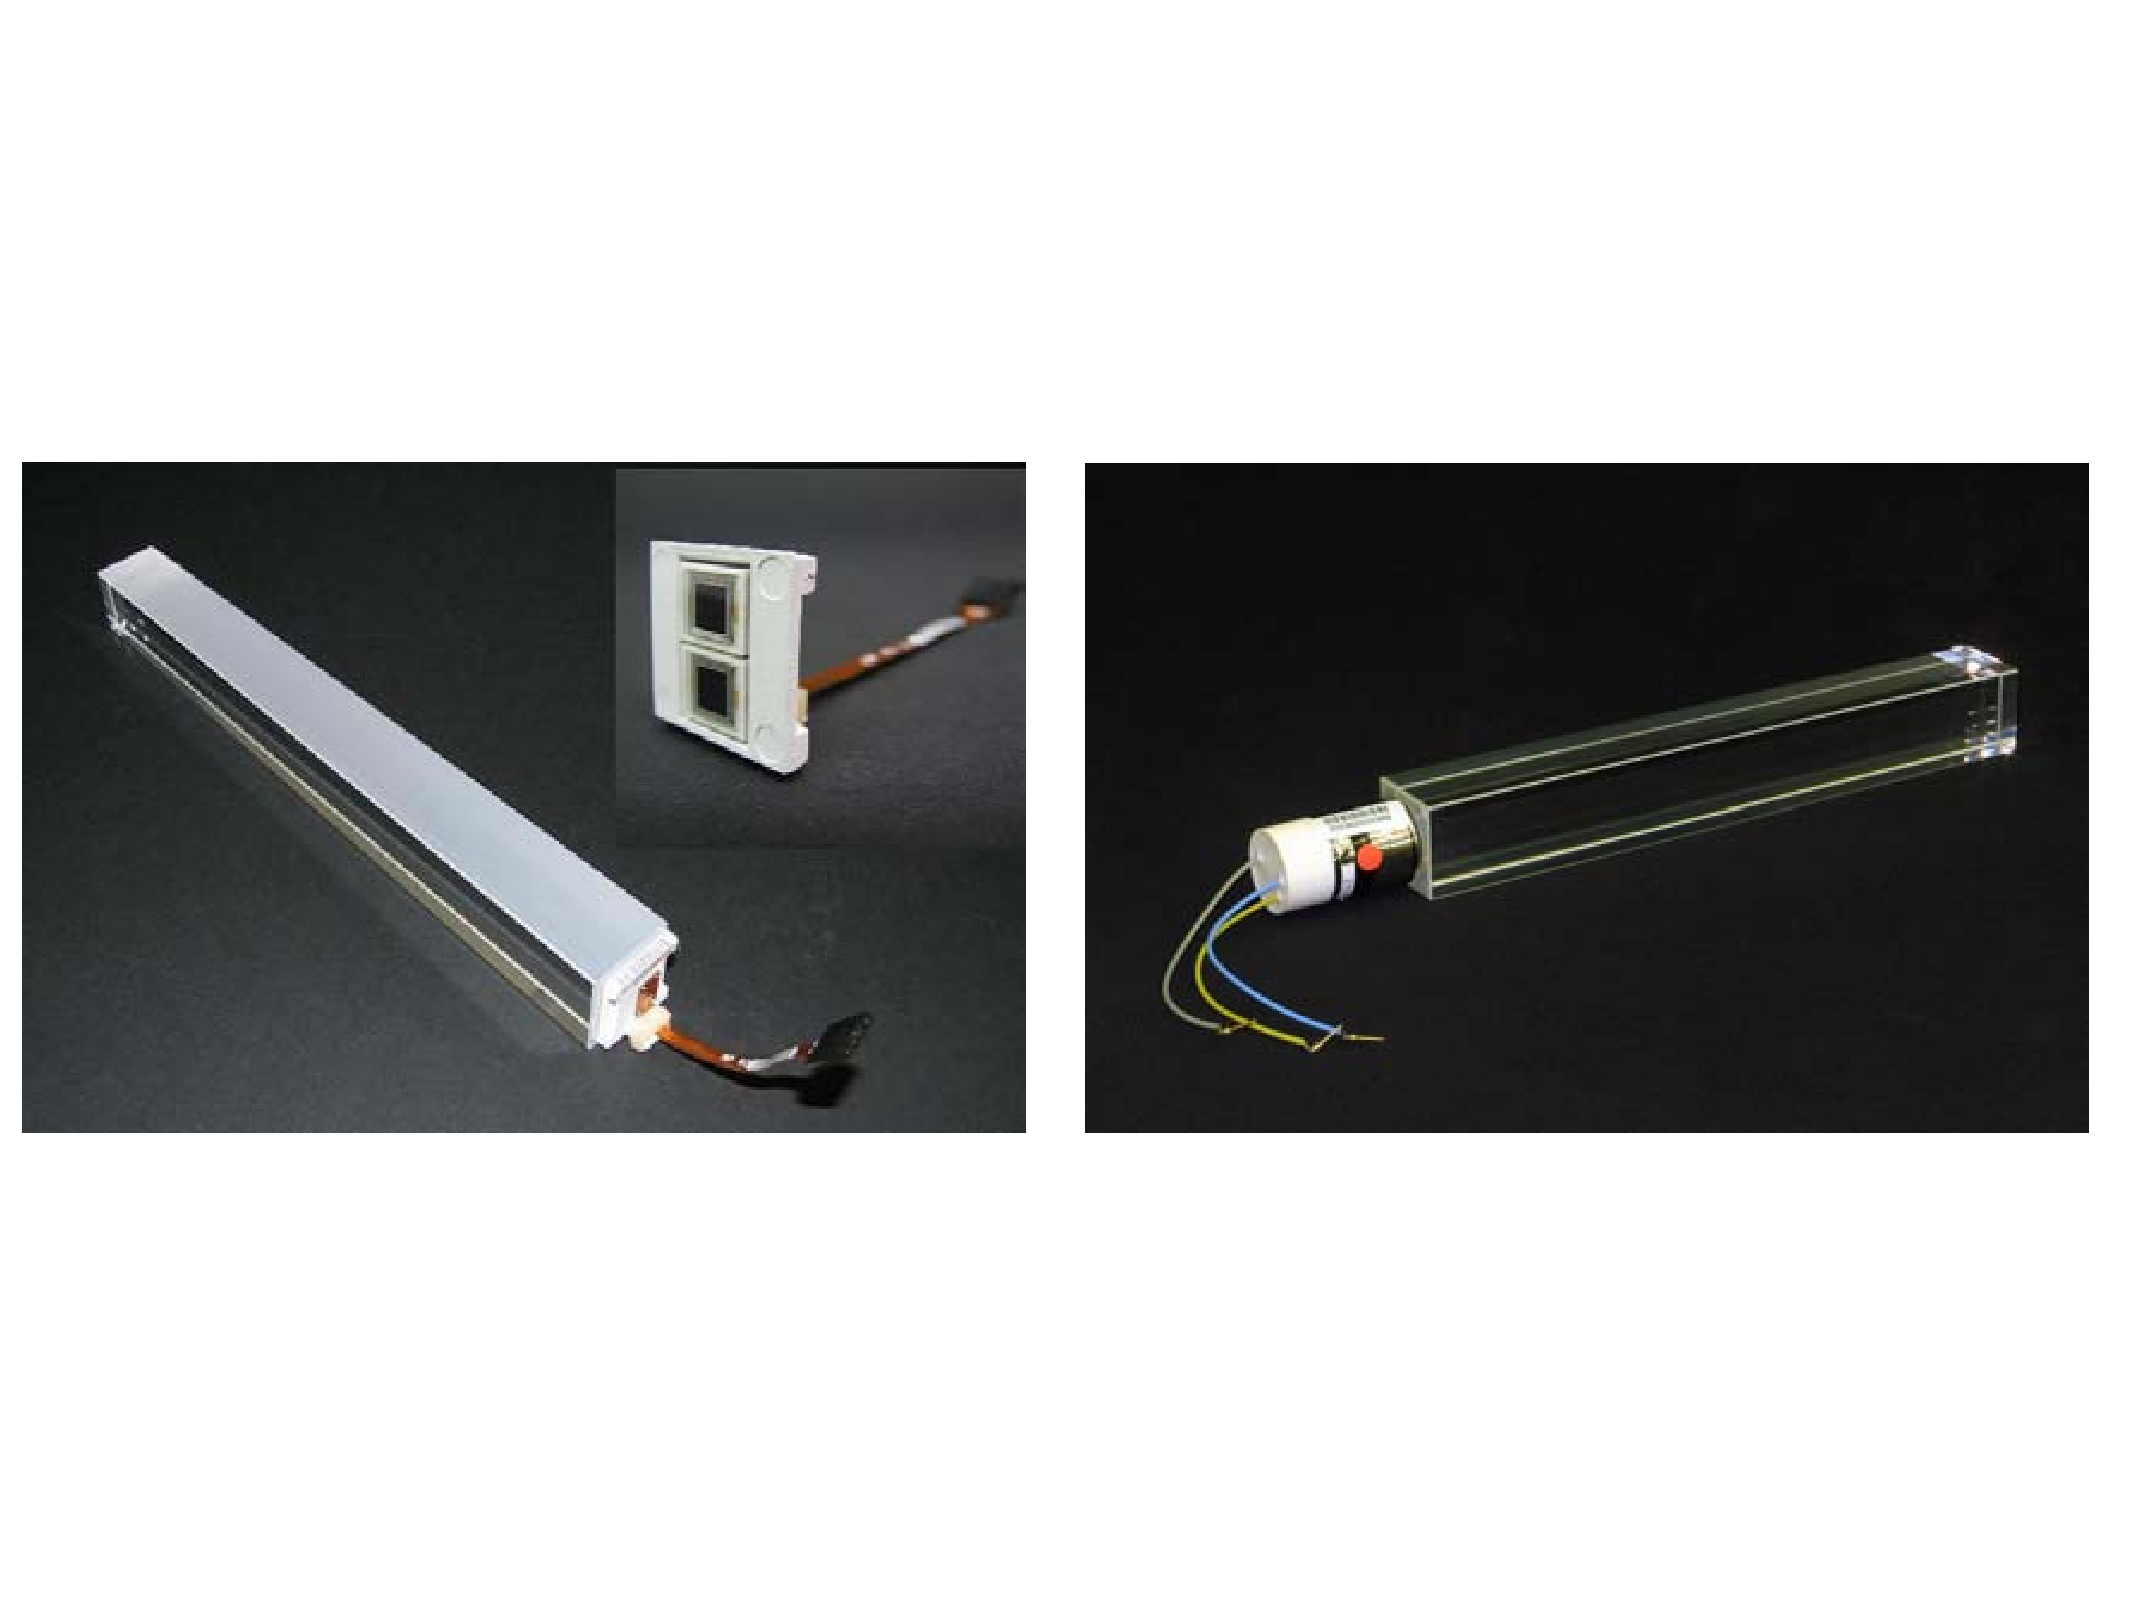
\includegraphics[width=0.99\textwidth]{CMS_DetectorFigures/EcalCrytals.pdf}
\caption{The  PbWO$_{4}$ crystal of the CMS ECAL, (left) a EB crystal
  instrumented with an APD and (right) a EE crystal instrumented with a VPT.\label{fig:ECALcrystals}}
\end{figure}
\begin{figure}
 \centering
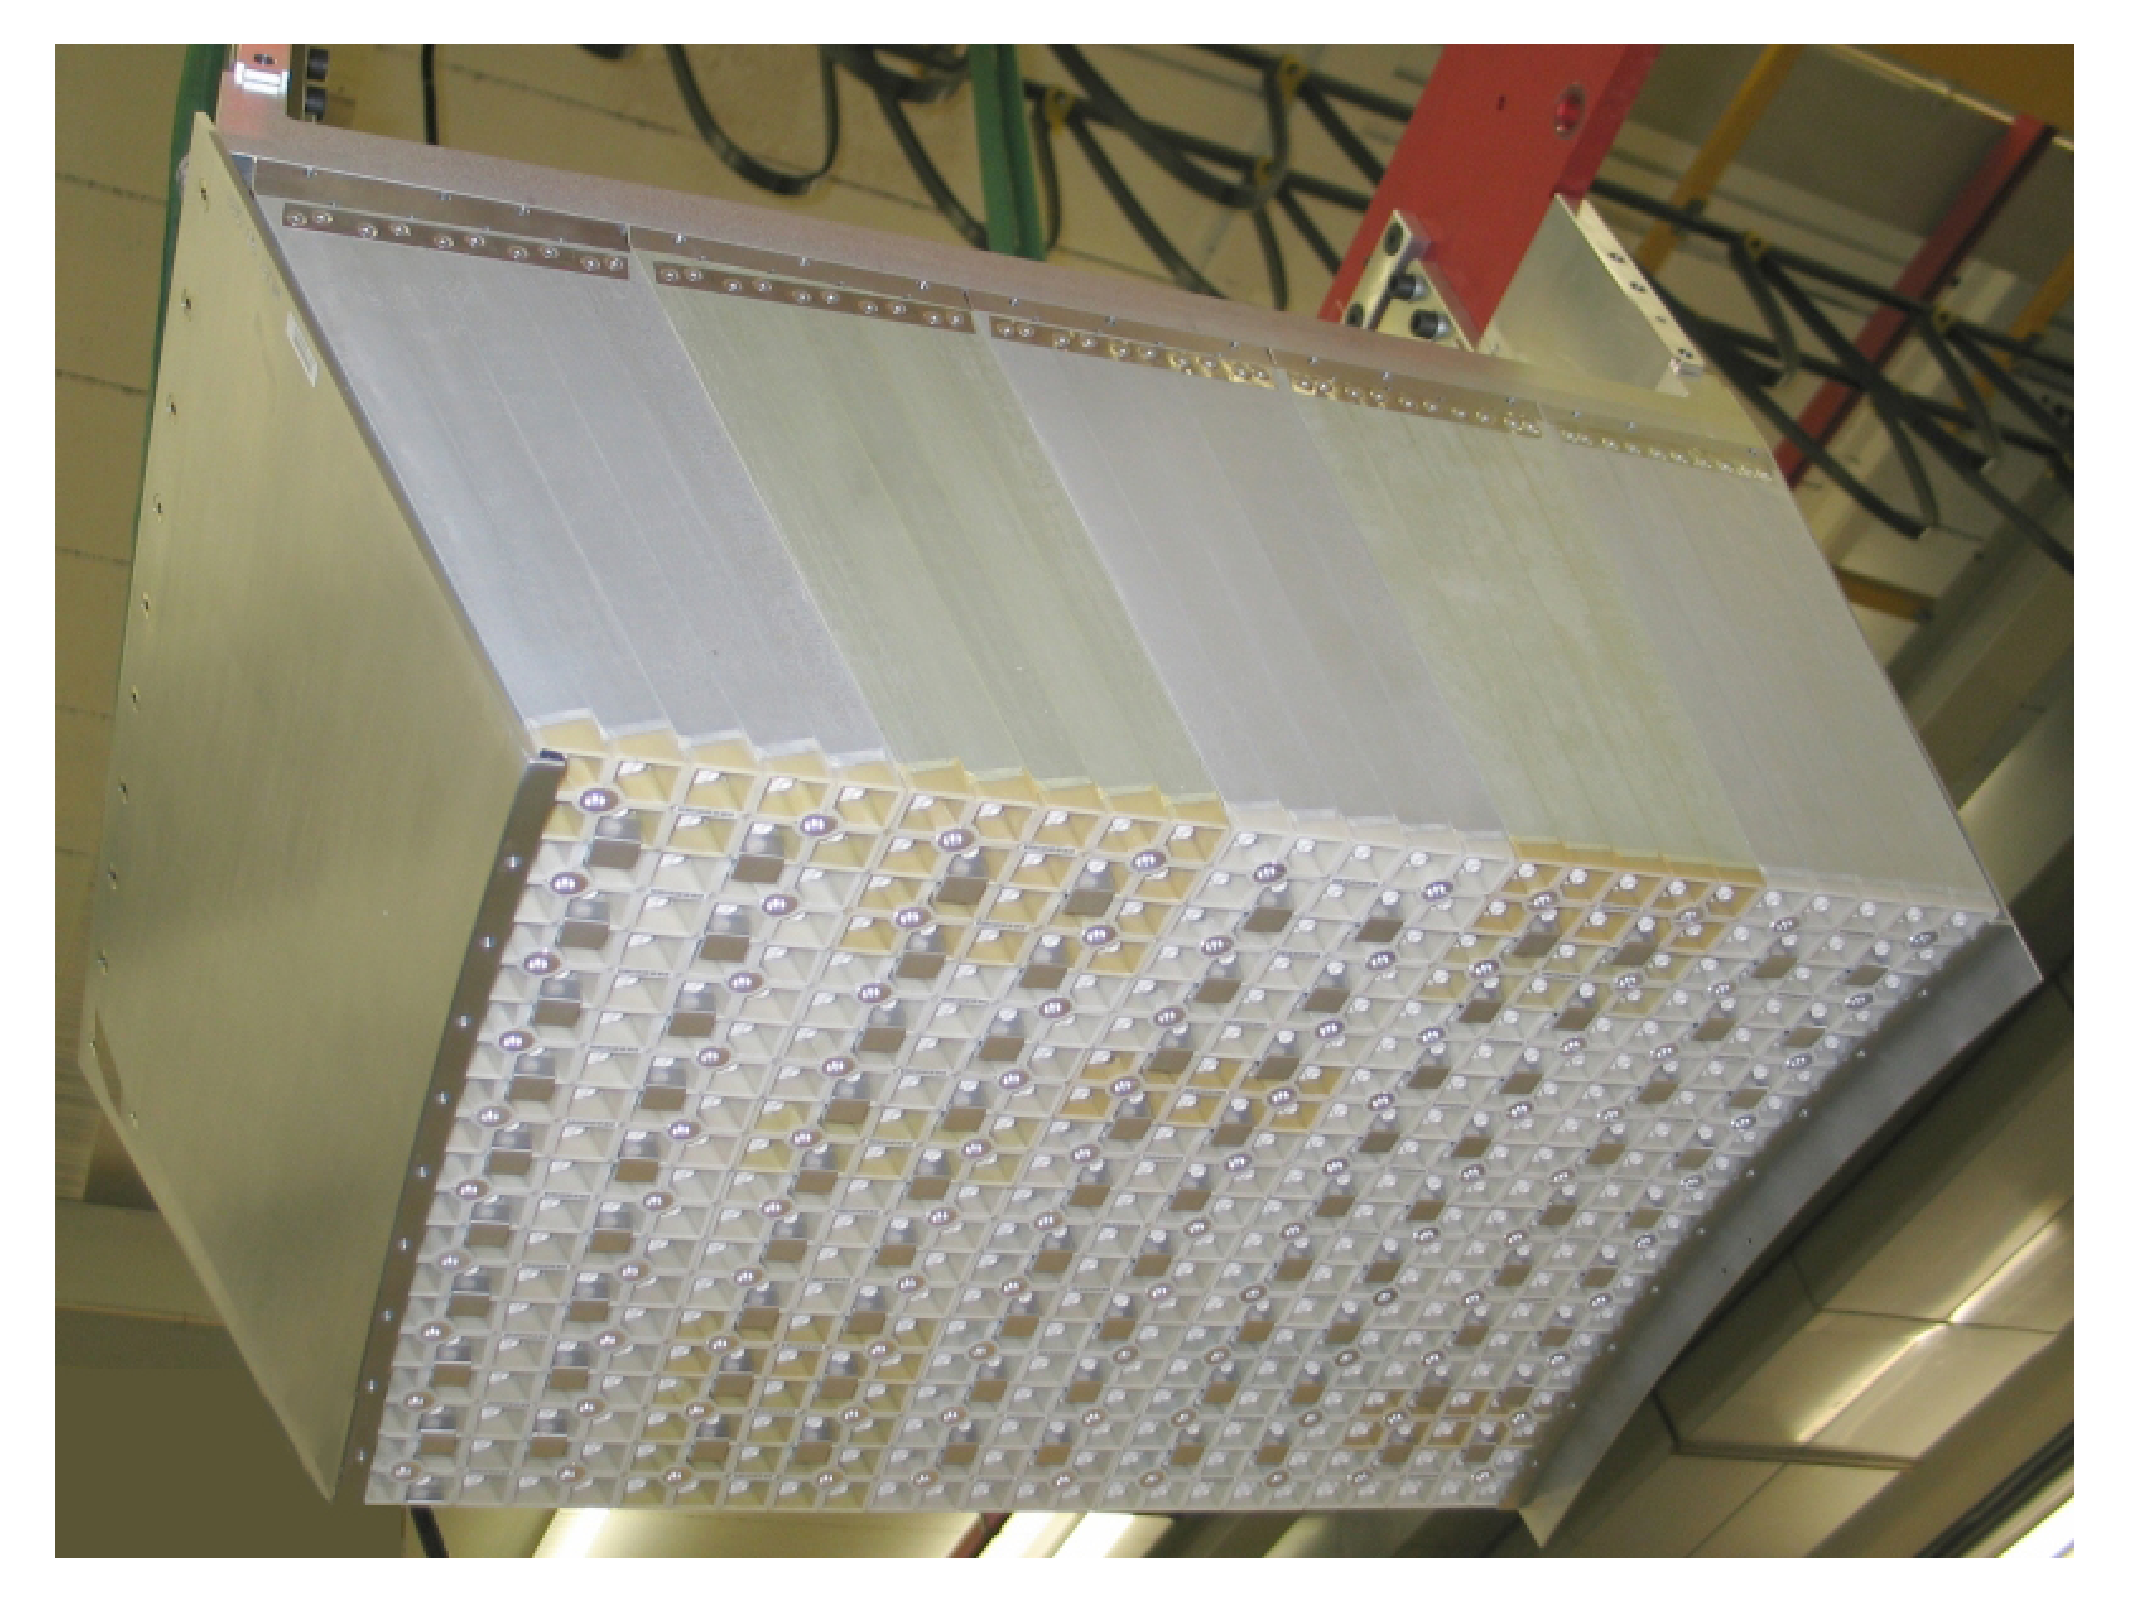
\includegraphics[width=0.99\textwidth]{CMS_DetectorFigures/ECALEB_Module.pdf}
\caption{A photograph of a EB module instrumented with crystals.\label{fig:ECALEB_module}}
\end{figure}
\begin{figure}
 \centering
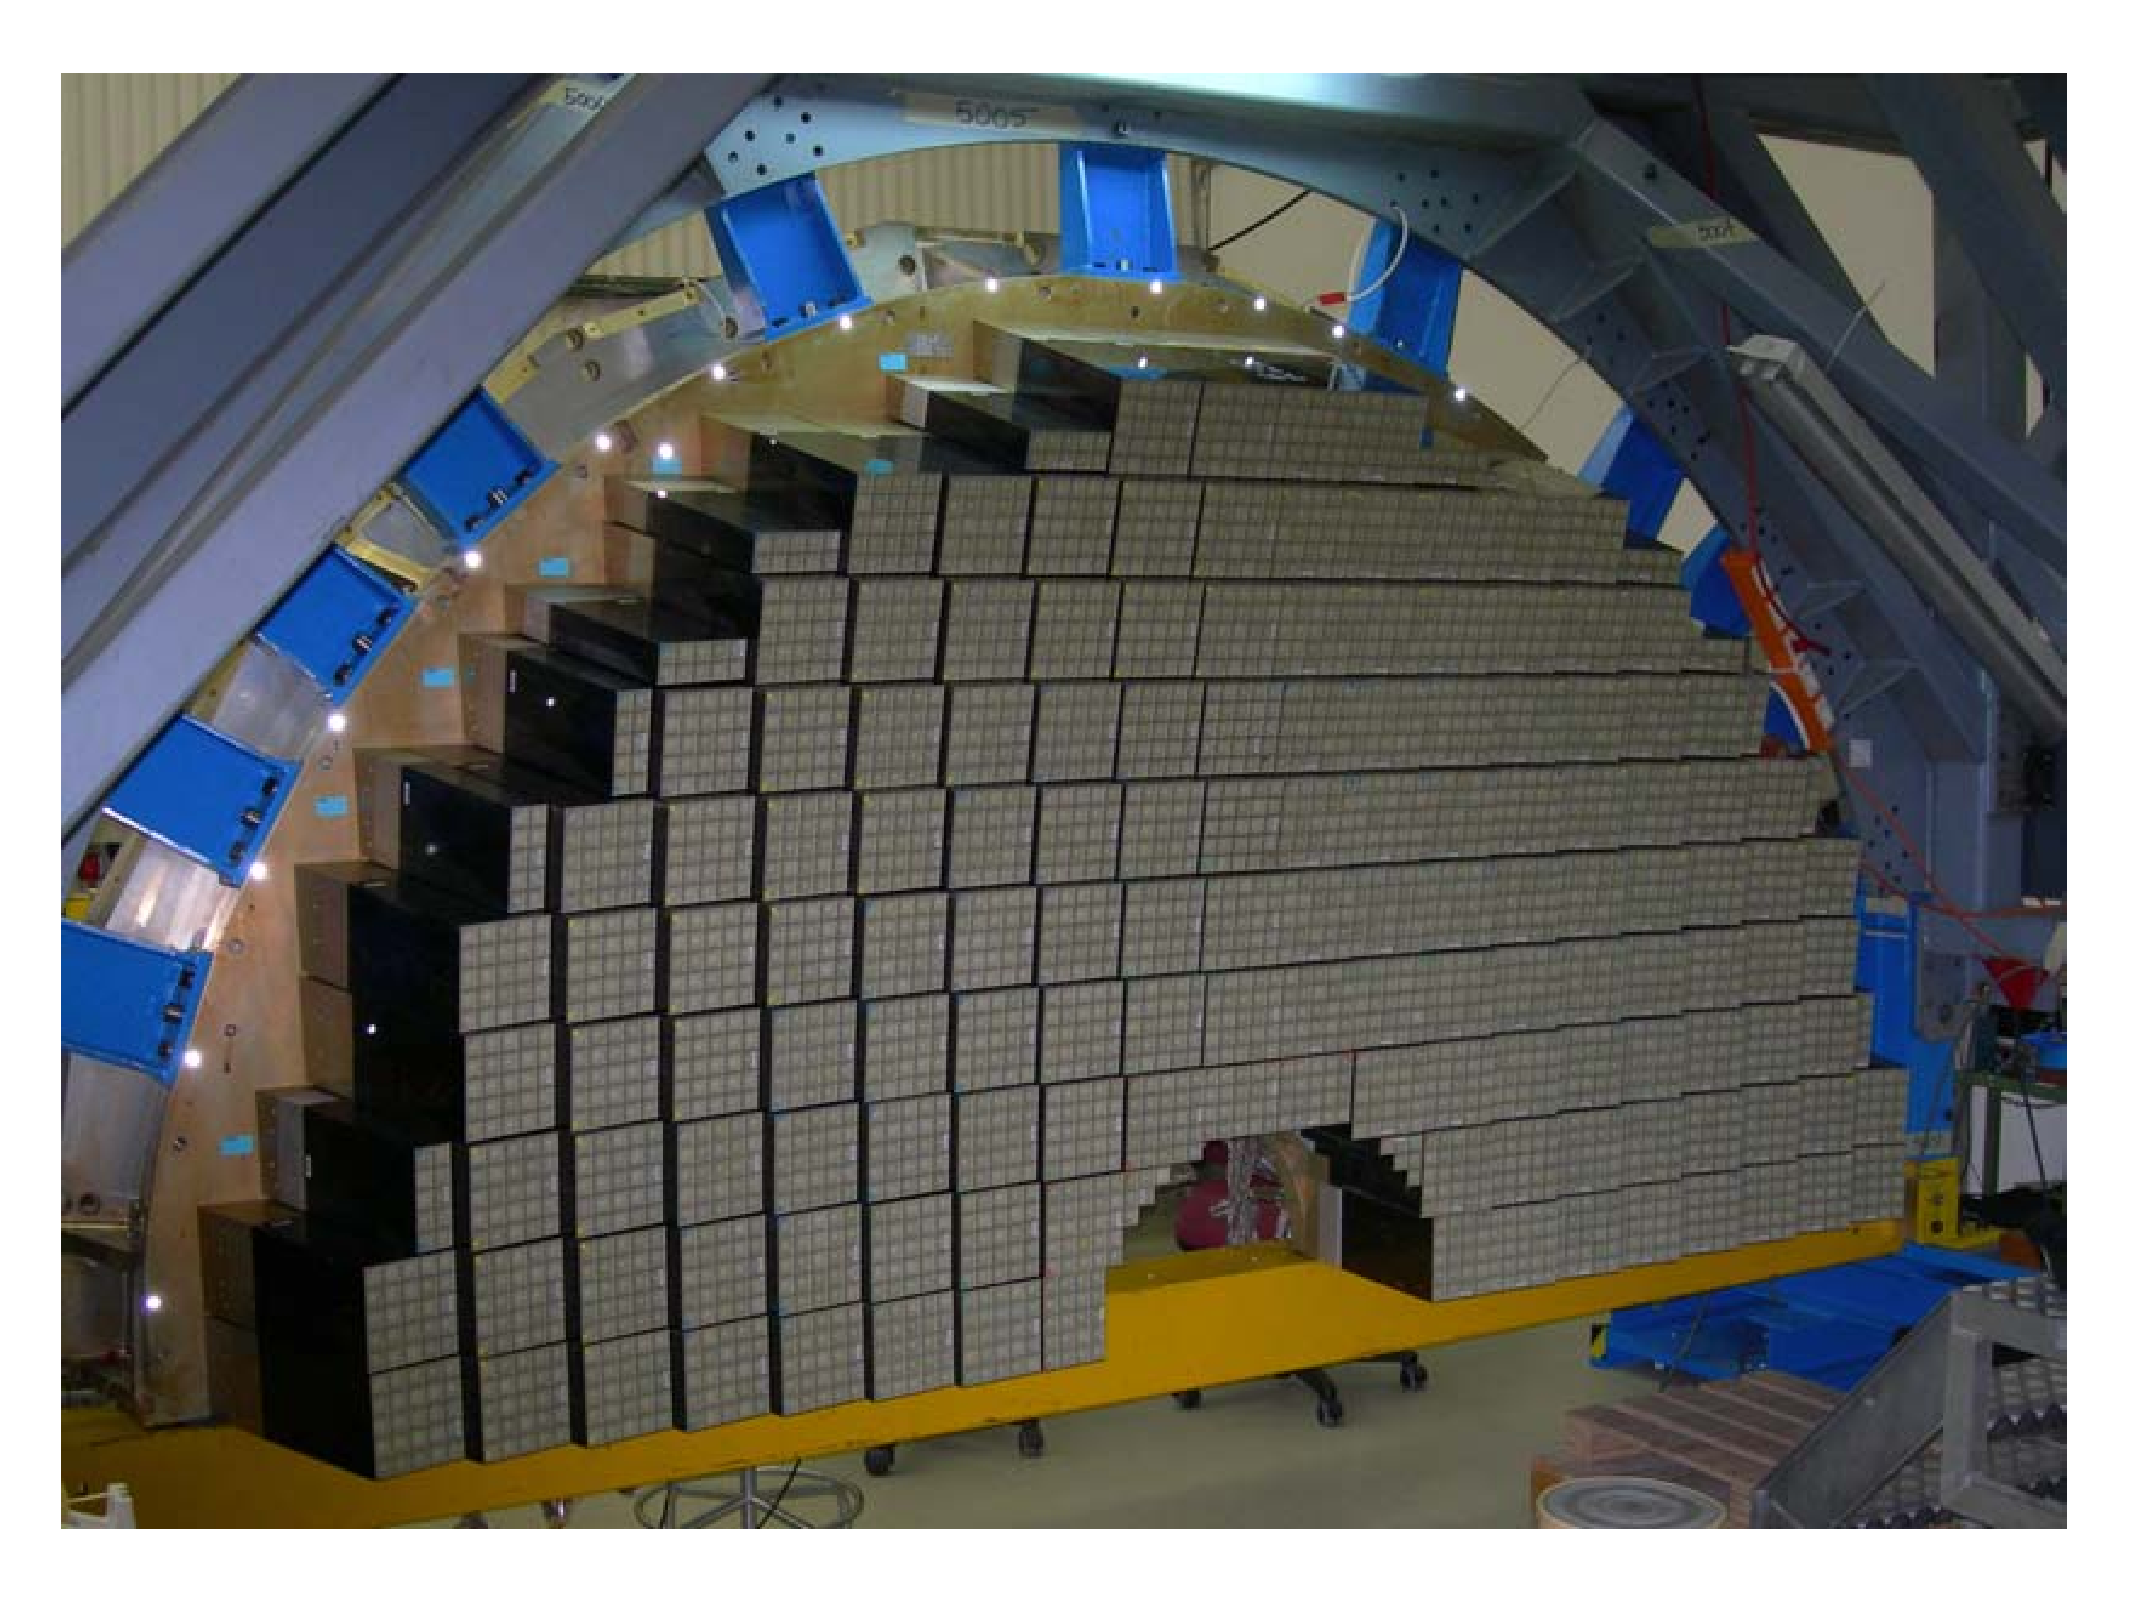
\includegraphics[width=0.99\textwidth]{CMS_DetectorFigures/ECALEE_Module.pdf}
\caption{A photograph of a EE Dee instrumented with crystals.\label{fig:ECALEE_module}}
\end{figure}
\subsection{ECAL Perfomance}

The EB has been extensively tested using electron beams, in this test
beam setup -- with no magnetic field or material in front -- the
energy resolution has been measured to be:
\begin{equation}\label{eq:ecalRes}
\frac{\sigma_{E}}{E} = \frac{2.8\%}{\sqrt{E(\GeV)}} \oplus
\frac{12\%}{E(\GeV)} \oplus 0.3\%,
\end{equation}

where E is the electron beam energy in units of \GeV. The terms in the
right-hand side of the Eq.~\ref{eq:ecalRes} are the so called
stochastic, noise, and constant terms. The first is due to the
fluctuations related to the development of the electromagnetic shower
inside the calorimenter crystals, the second is dues to electronic
noise of the readout chain, and the last is related to the
instrumental effect such as non-linear response, radiation damage,
shower leakage among others.

The test beam ideal conditions clearly differ from those at the CMS
experiment and therefore in situ measurements of the performance of
the ECAL have been performed durin the data-taking period at 7 and
8\TeV. One key measurement is the trigger efficiency for
electron/photon (e/$\gamma$) candidates, the Level-1 trigger was
operated with a threshold of $E_{T}$ = 20\GeV (provided by 5$\times$5
crystals) in 2012 and found to be above 99\% efficienct for $E_{T}$ >
40\GeV, thus enabling a fully efficienct H$\rightarrow\gamma\gamma$
search.

The e/$\gamma$ energy measurement depends upon the correct
reconstruction of electromagnetic showers in the ECAL. Some e/$\gamma$
candidates interact -- by bremsstrahlung or photon conversion -- with
the silicon tracker  prior reaching the ECAL or their trajectories are
modified due to the 3.8 T magnetic field causing the showers to spread
on the azhimutal direction and thus their energy is shared by multiple
crystals. In order to account for these effect and ensure a more
accurate e/$\gamma$ reconstruction a dynamic clustering algorithim is
used to merge clusters of energy deposited that belong to the same
electromagnetic shower into the so-called \textit{superclusters}
(SCs). Once the SC is formed, the e/$\gamma$ candidate energy
($E_{e/\gamma}$) is reconstructed using the following expression:

\begin{equation}
\label{eq:ecalE}
E_{e/\gamma} = F_{e/\gamma}\cdot \big(G\cdot\sum S_{i}(t)C_{i}A_{i} + E_{\mathrm{ES}}\big)
\end{equation}
 
where $F_{e/\gamma}$ is a correction accounting for the imperfect
clustering, material, and geometric efffect; $G$ is the ADC-to-\GeV
conversion; $S_{i}(t)$ is the time-dependent correction to account for
the response variations of the $i$-th crystal; $C_{i}$ is the
inter-calibration coefficient of the $i$-th crystal; $A_{i}$ is the
amplitude of the $i$-th crystal in ADC counts; finally,
$E_{\mathrm{ES}}$ is the pre-shower energy -- only relevant for
e/$\gamma$s in the EE. Figure~\ref{fig:ECAL_clusterE} shows the effect
of the clustering process and the application of the $F_{e/\gamma}$
correction by comparing the invariant mass of $e^{+}e^{-}$ pairs
coming from a Z boson with respect to the usage of the simple fixed
5$\times$5 cluster energy.

\begin{figure}
 \centering
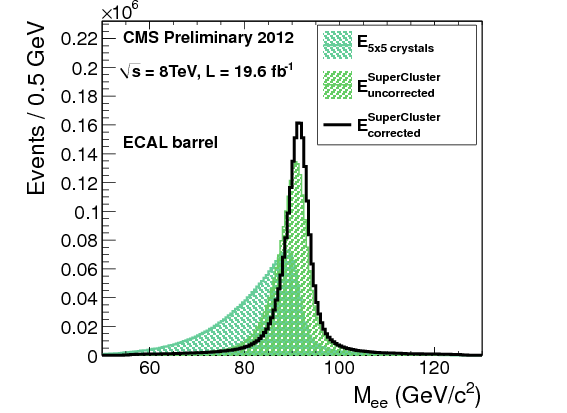
\includegraphics[width=0.49\textwidth]{CMS_DetectorFigures/E_corr-EB.png}
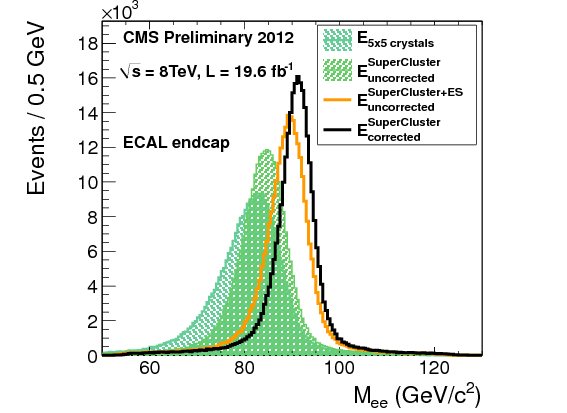
\includegraphics[width=0.49\textwidth]{CMS_DetectorFigures/E_corr-EE.png}
\caption{The reconstructed Z invariant mass from $e^{+}e^{-}$
  decays. The left and right panels show the reconstructed invariant mass for
  the EB and EE, repectively, with different algorithms to reconstructed electron energies.\label{fig:ECAL_clusterE}}
\end{figure}

The inter-calibration coefficient is responsible for correcting the
channel-to-channel variation in response. The main sources for such
variations are the crystal light yield variations ( up to $\sim$ 15\%)
and the spread on the gain of the photodetectors ( up to $\sim$
25\%). An inter-calibration is carrried out in situ by methods that
explote the time- and $\phi$-invariance of the energy flow in the
crystals at a given $\eta$ in minimum-bias events, as well as the
$\pi^{0}/eta$ mass constraint to the photons pair from its decay, and
the momentum constraint of isolated electrons from W and Z boson
decays. The precision of these methods as a function of $\eta$ is
shown in Figure~\ref{fig:ECAL_ICPrecision}. The invariant mass of
diphotons consistent with a $\pi^{0}$ and $\eta$ used in the
inter-calibration is shown in the left and right panels of
Figure~\ref{fig:ECAL_pizero}, respectively.

\begin{figure}
 \centering
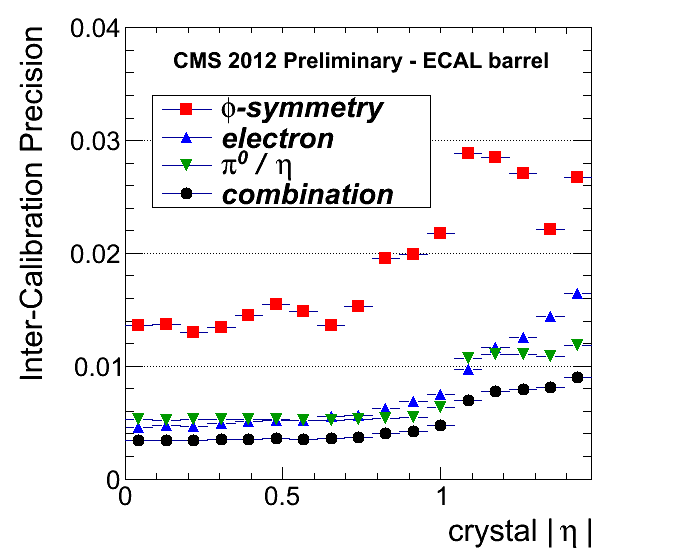
\includegraphics[width=0.49\textwidth]{CMS_DetectorFigures/2012EBprecWithCombV3.png}
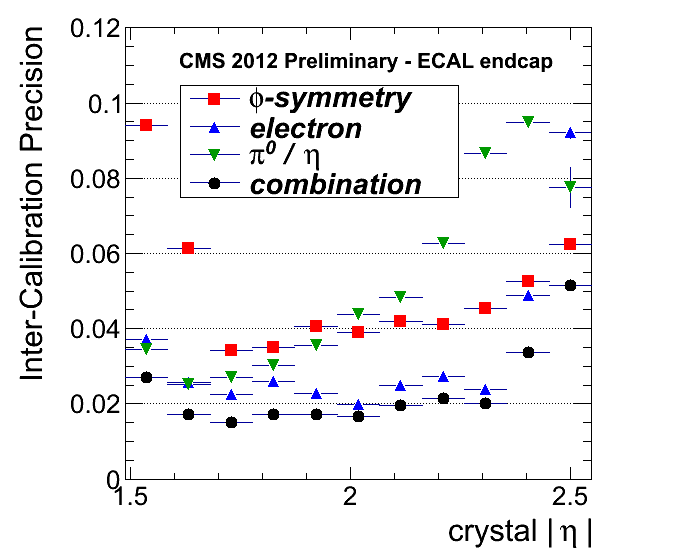
\includegraphics[width=0.49\textwidth]{CMS_DetectorFigures/2012EEprecWithCombV3.png}
\caption{The reconstructed Z invariant mass from $e^{+}e^{-}$
  decays. The left and right panels show the reconstructed invariant mass for
  the EB and EE, repectively, with different algorithms to reconstructed electron energies.\label{fig:ECAL_ICPrecision}}
\end{figure}

\begin{figure}
 \centering
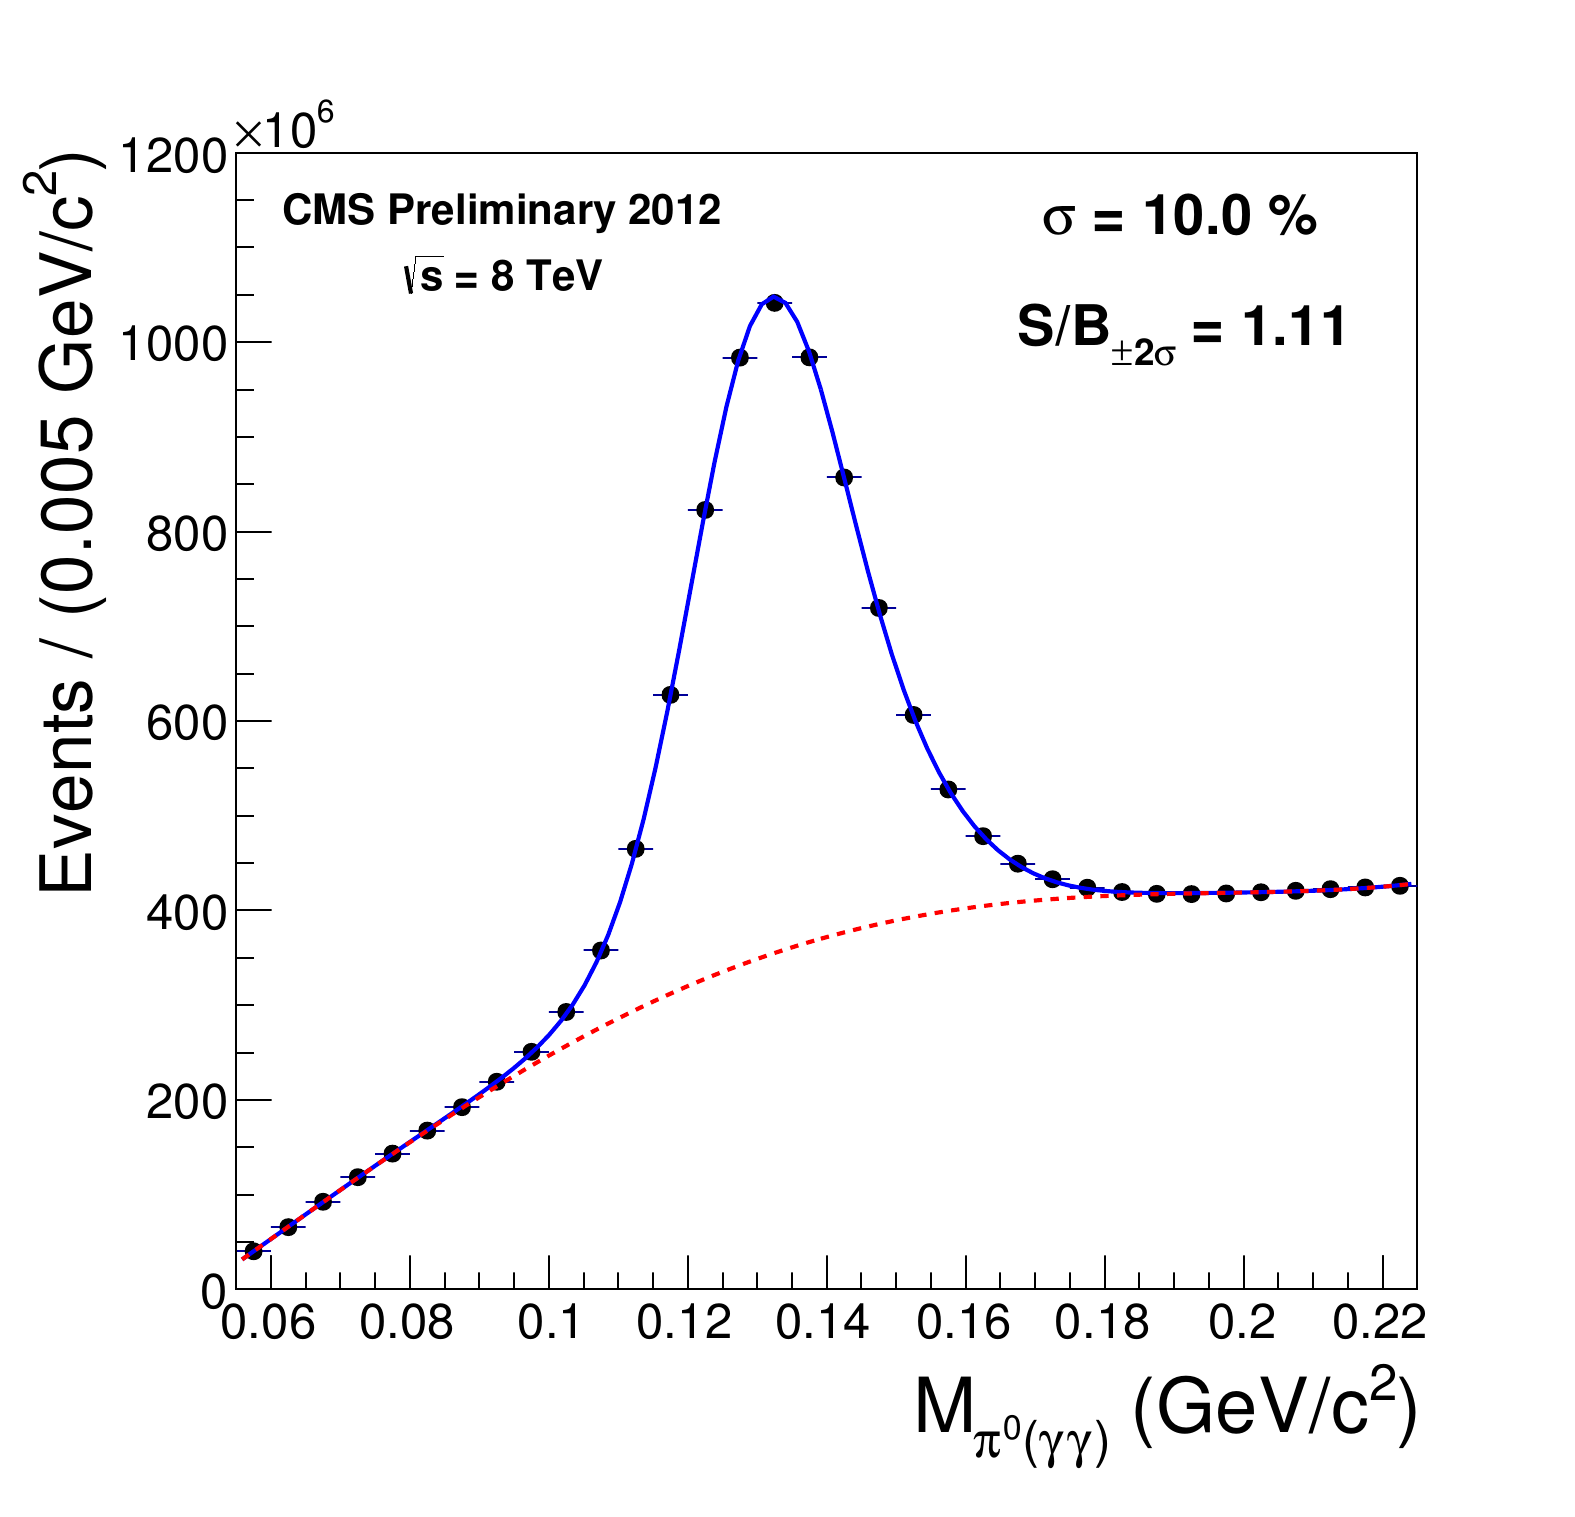
\includegraphics[width=0.49\textwidth]{CMS_DetectorFigures/EB_2012_pi0.png}
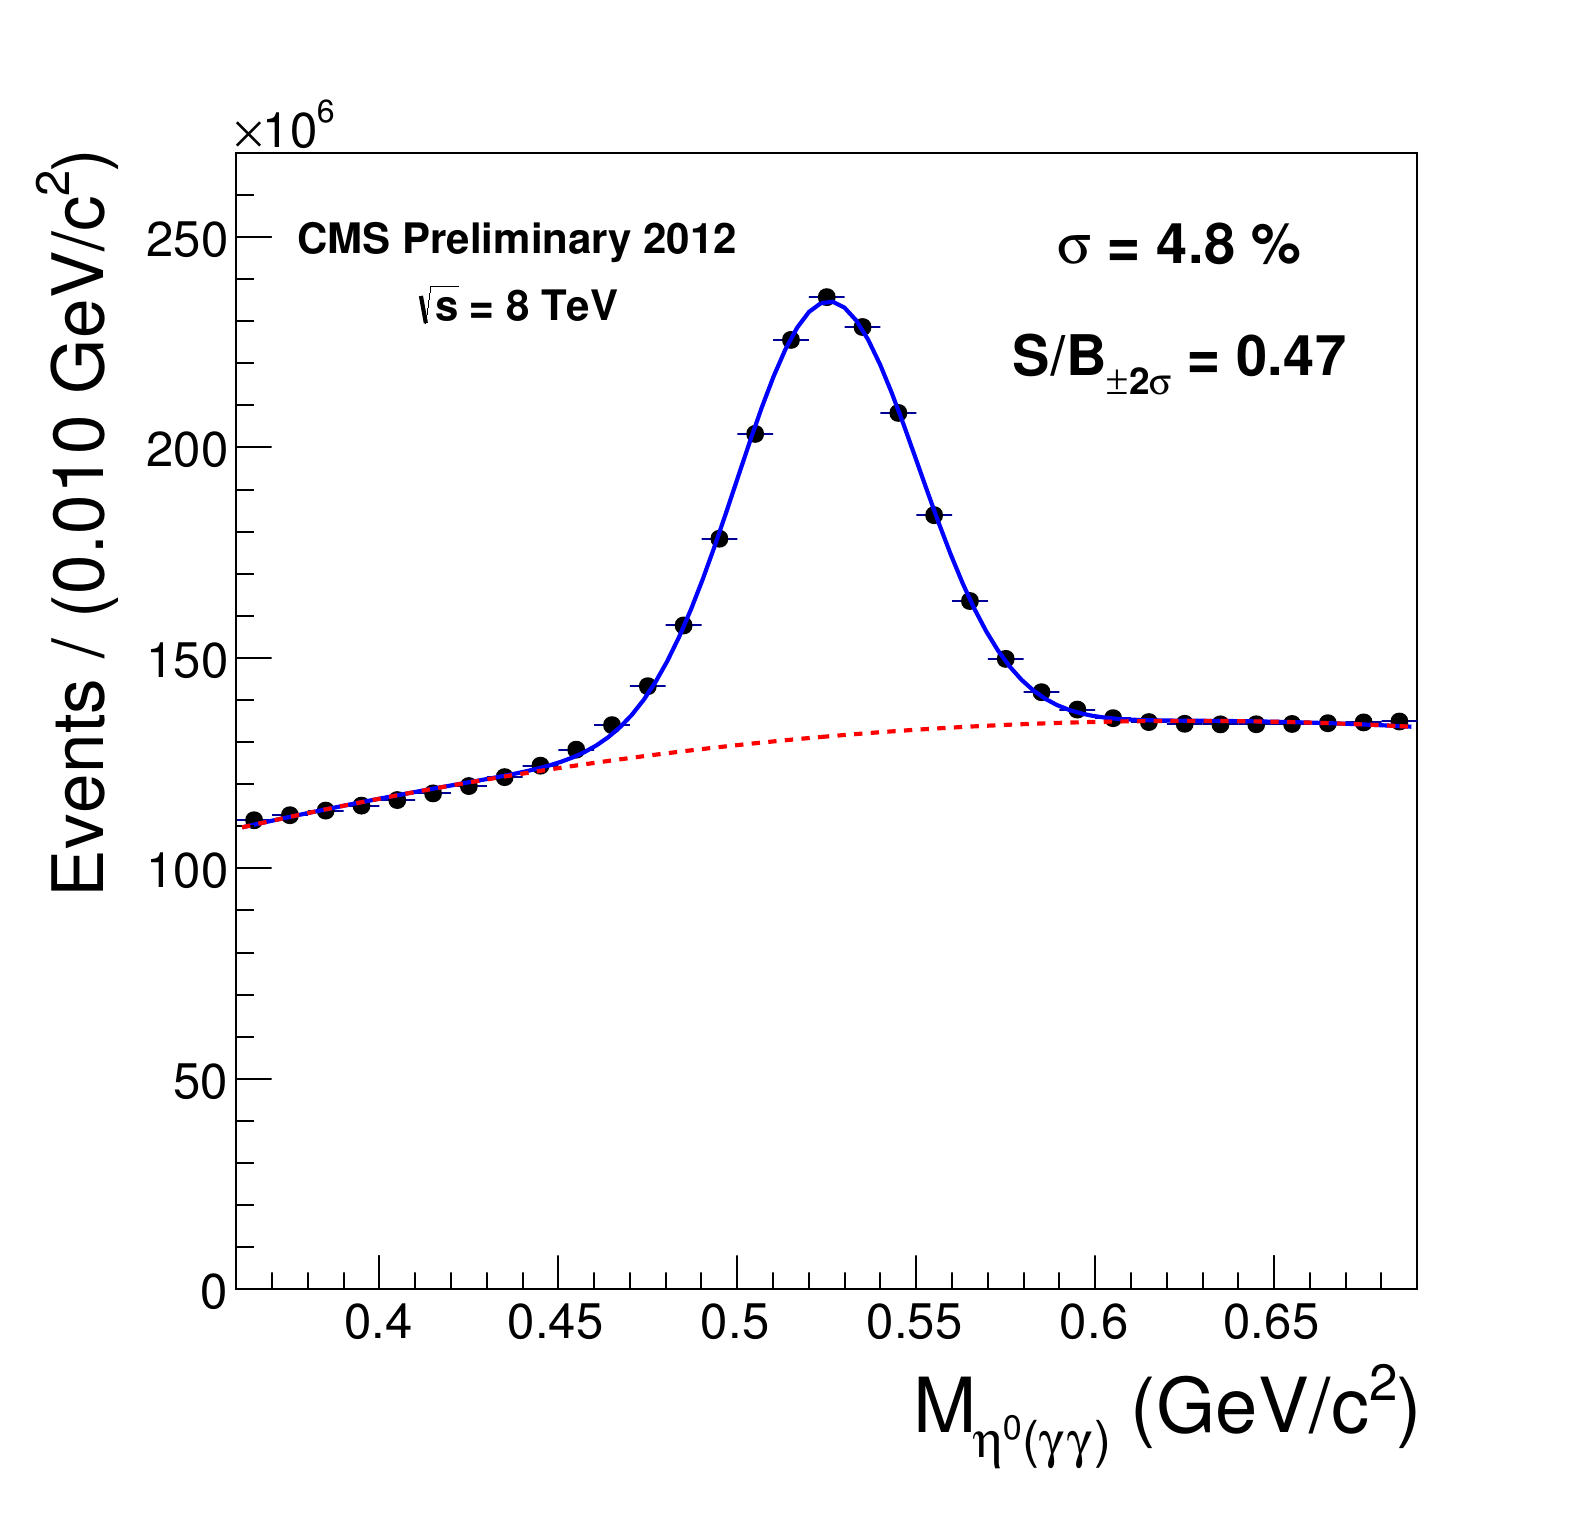
\includegraphics[width=0.49\textwidth]{CMS_DetectorFigures/EB_2012_eta0.png}
\caption{The reconstructed Z invariant mass from $e^{+}e^{-}$
  decays. The left and right panels show the reconstructed invariant mass for
  the EB and EE, repectively, with different algorithms to reconstructed electron energies.\label{fig:ECAL_pizero}}
\end{figure}
Another important ingredient to the precise measurement of the
electromagnetic shower energy is the time dependent corrections, at
CMS the ECAL crystals undergo changes in transparency due to the
radiation received while collisions occur, while  during downtime the
transparency is recovered. In order to correct for the transparency
changes a laser monitoring system is installed and run every $\sim$40
minutes. Laser light ($\lambda = 440$ nm) close to the emission peak of PbWO$_{4}$
is impinge into all the crystals, thus, tracking their response
variations. The variations on transparency as a function of time for
different $\eta$ ranges is shown in
the left panel of Figure~\ref{fig:ECAL_Transparency1}, where it is observed that the
transparency variations are more severe at large pseudorapidities. The
validity of the laser monitoring (LM) correction is checked using
electrons from W decays. The stability of the LM correction is
estimated by the rms of the $E/p$ ratio in these events and found to
be about 0.1\% and 0.3\% for the EB and EE, respectively. The right
panel of Figure~\ref{fig:ECAL_Transparency1} shown the LM correction
effect on electron from W events in the EE. The effect of the
inter-calibration and LM corrections is shown Figure~\ref{fig:ECAL_E_IC_LM}, where
the invariant mass of $e^{+}e^{-}$ pairs from Z decays is
reconstructed with and without such corrections being applied.
\begin{figure}
 \centering
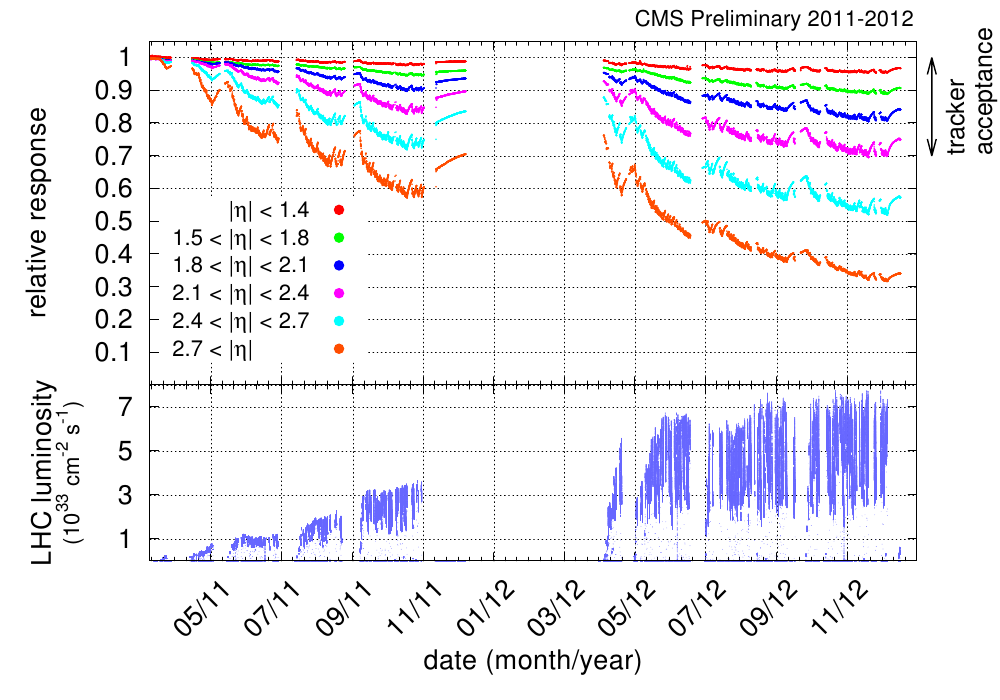
\includegraphics[width=0.99\textwidth]{CMS_DetectorFigures/histories_2011-2012.png}
\caption{The reconstructed Z invariant mass from $e^{+}e^{-}$
  decays. The left and right panels show the reconstructed invariant mass for
  the EB and EE, repectively, with different algorithms to reconstructed electron energies.\label{fig:ECAL_Transparency1}}
\end{figure}

\begin{figure}
 \centering
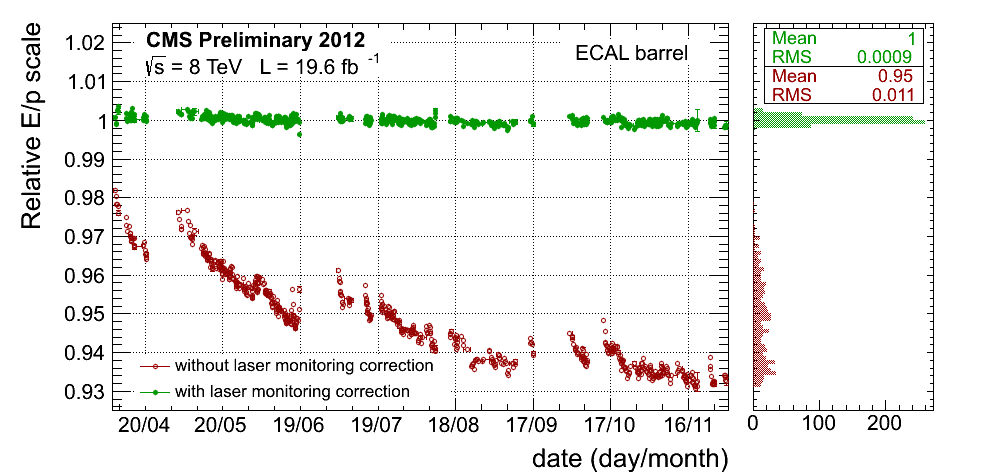
\includegraphics[width=0.99\textwidth]{CMS_DetectorFigures/approval_EB_Winter2013.png}
\caption{The reconstructed Z invariant mass from $e^{+}e^{-}$
  decays. The left and right panels show the reconstructed invariant mass for
  the EB and EE, repectively, with different algorithms to reconstructed electron energies.\label{fig:ECAL_response}}
\end{figure}

\begin{figure}
 \centering
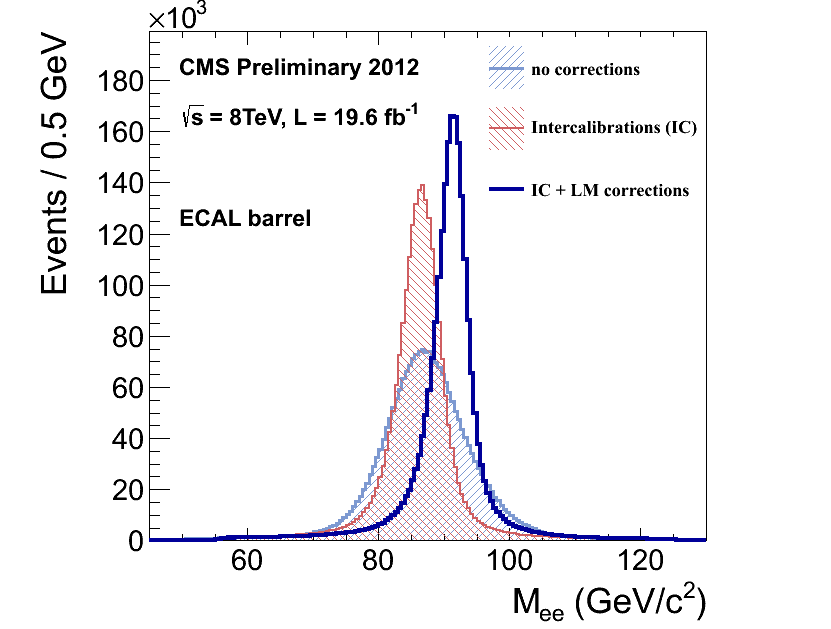
\includegraphics[width=0.49\textwidth]{CMS_DetectorFigures/noIC_noLaser-regrCorr_ele-EB.png}
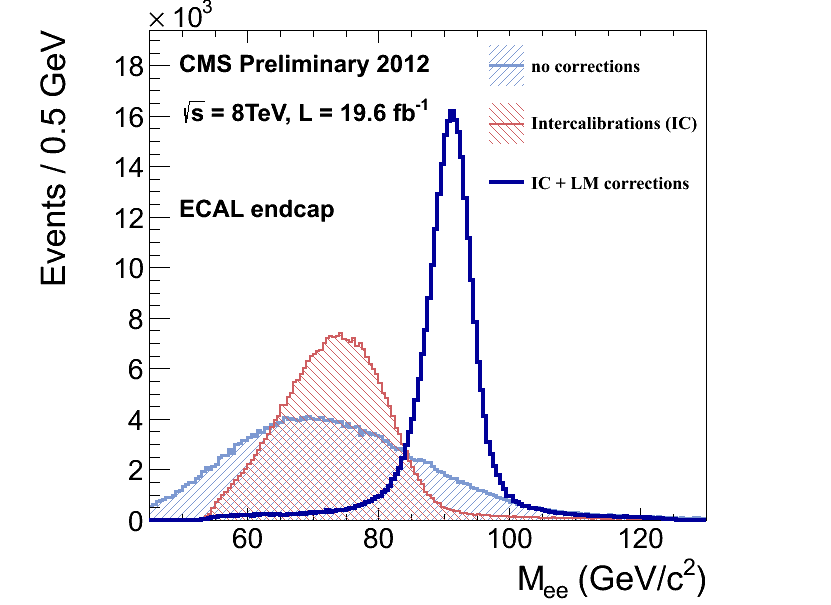
\includegraphics[width=0.49\textwidth]{CMS_DetectorFigures/propaganda_noIC_noLaser-regrCorr_ele-EE.png}
\caption{The reconstructed Z invariant mass from $e^{+}e^{-}$
  decays. The left and right panels show the reconstructed invariant mass for
  the EB and EE, repectively, with and without the IC and the LM corrections.\label{fig:ECAL_E_IC_LM}}
\end{figure}
 Finally, the overall energy resolution of the CMS ECAL has been measured
 and compared to simulation, this is shown in the right panel of
 Figure~\ref{fig:ECAL_Higgs}. The energy resolution is found to be
 between 1-2\% for $|\eta|<1$ and between 3-5\% in the EE, it is also
 observed that the simulation and measurement do not agree and that an
 extra constant term as a function of $\eta$ should be added to the
 simulation. The performance of the ECAL can also be observed in the
 width of the invariant mass of the Higgs boson, this is shown in the
 left panel of Figure~\ref{fig:ECAL_Higgs}, where a $\sigma_{eff}$ =
 1.36\GeV is observed.
\begin{figure}
 \centering
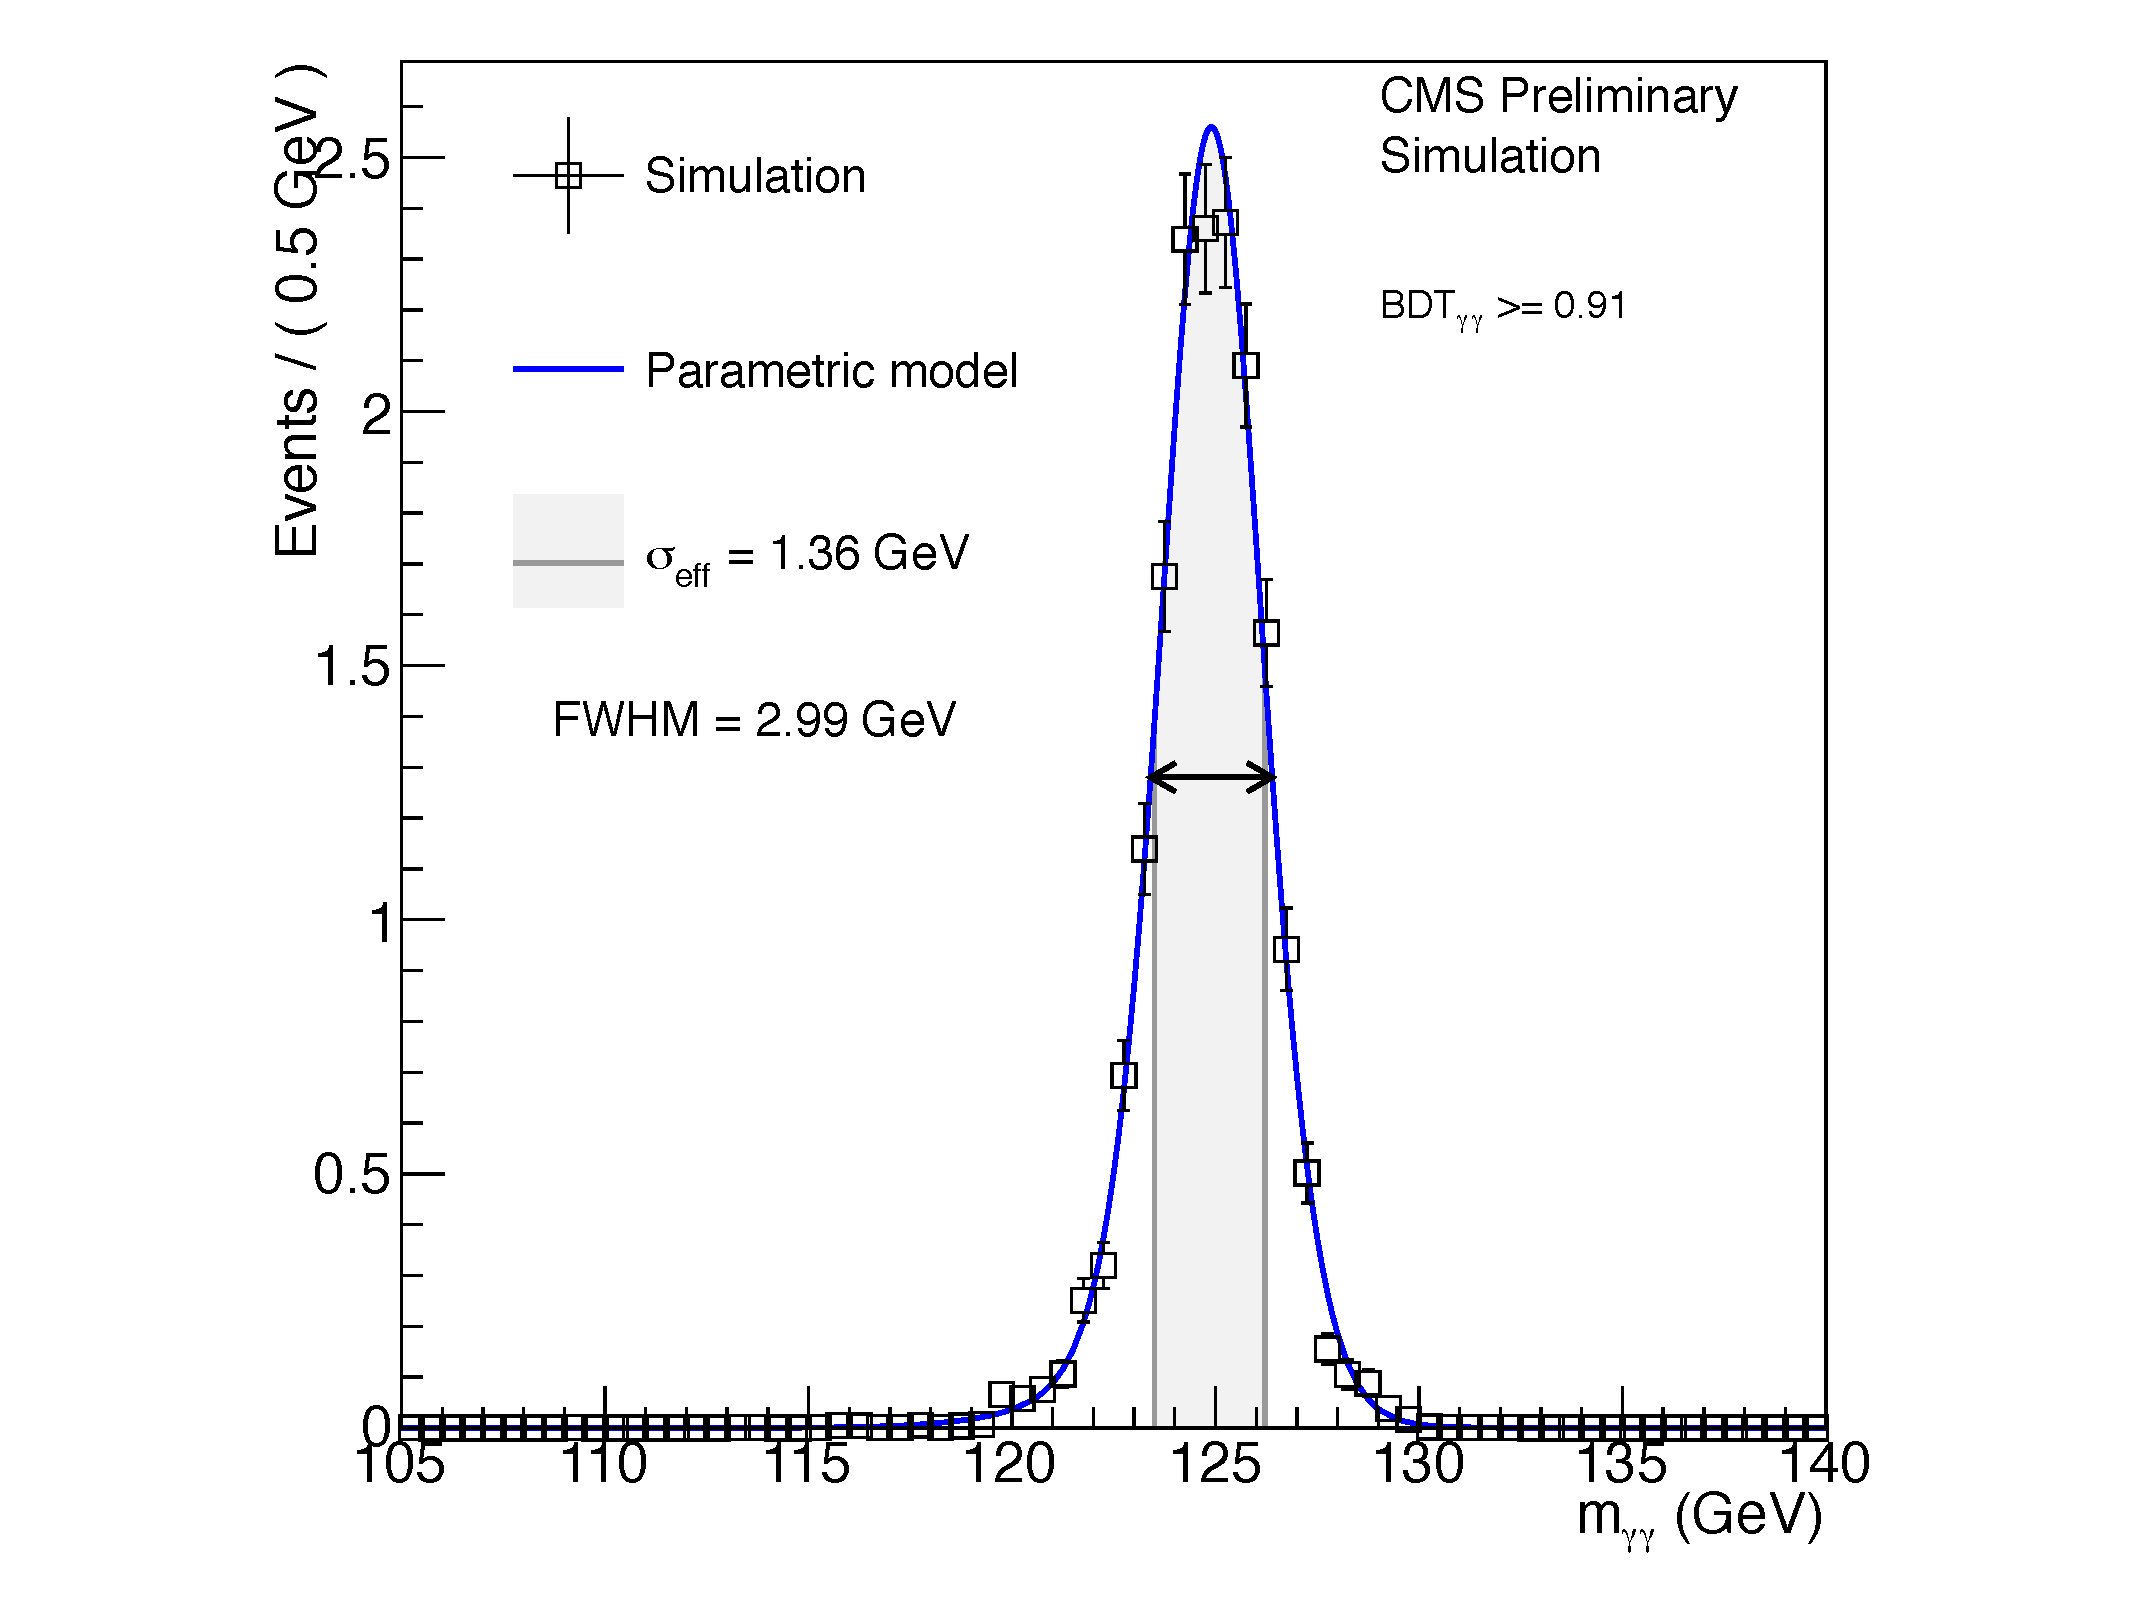
\includegraphics[width=0.38\textwidth]{CMS_DetectorFigures/ECAL_HiggsMassRes.pdf}
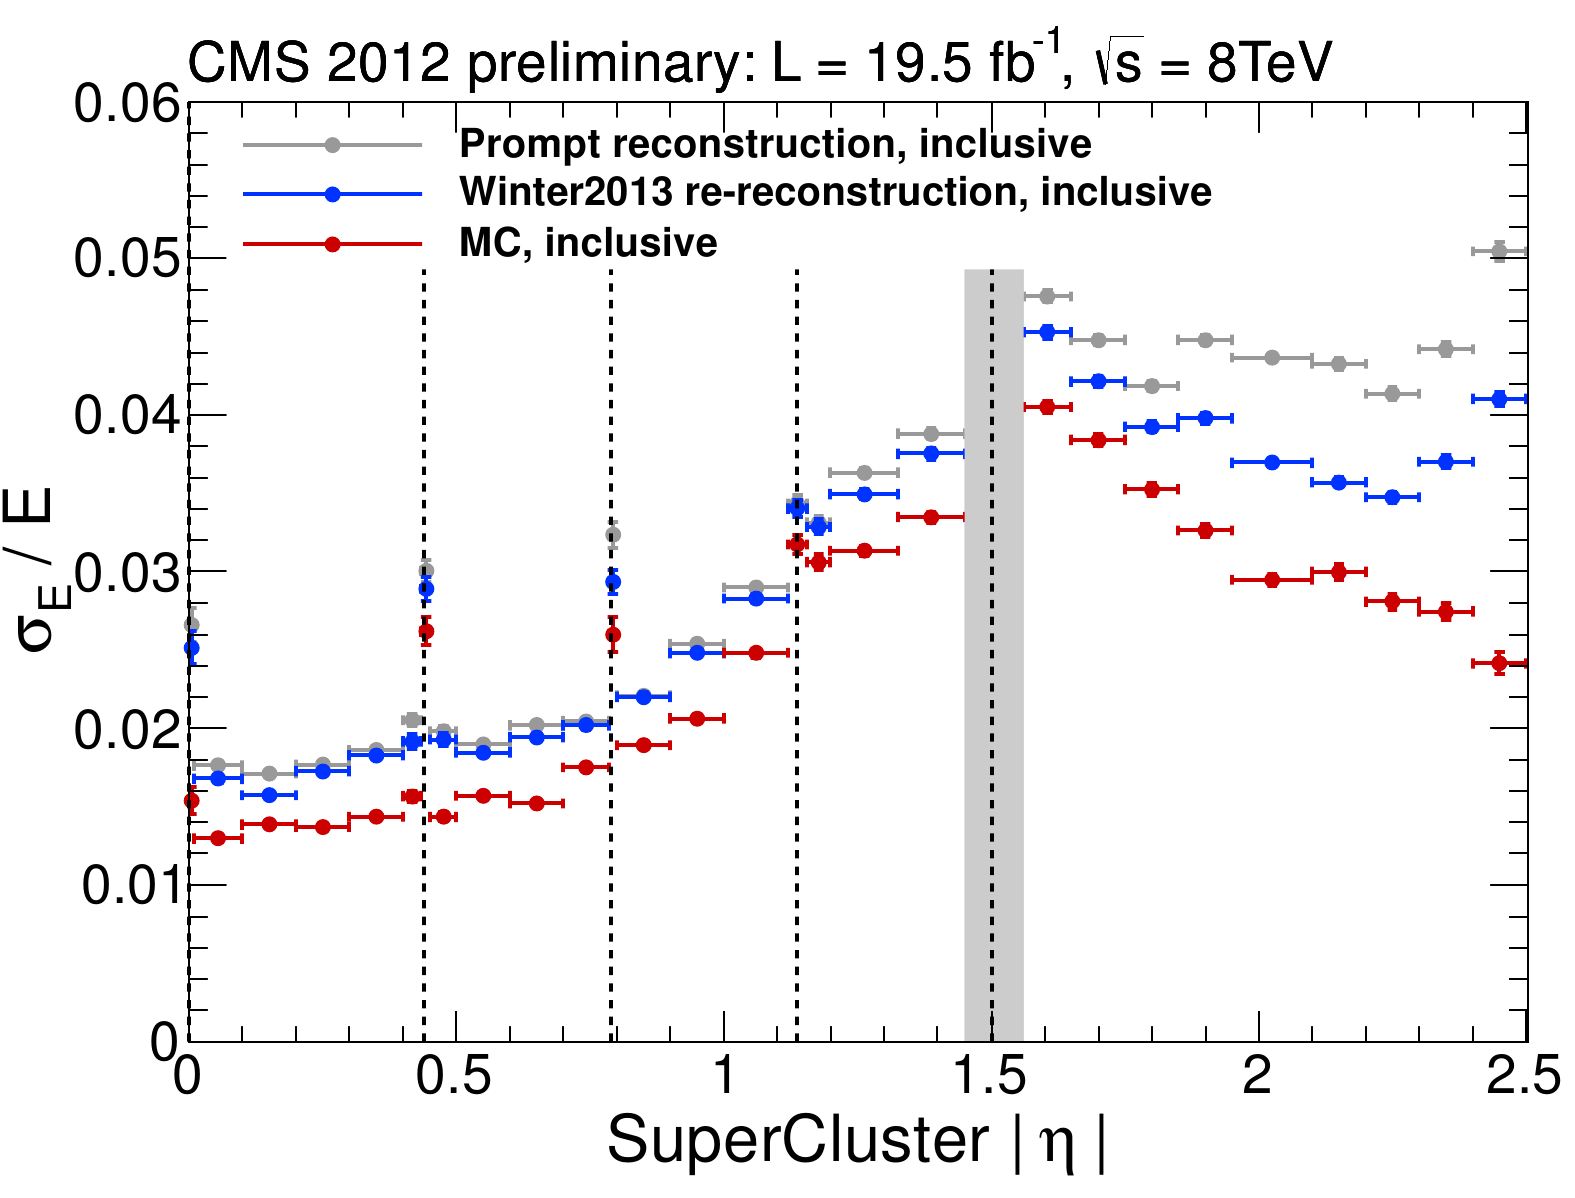
\includegraphics[width=0.49\textwidth]{CMS_DetectorFigures/EcalScaleEta_Incl.png}
\caption{The reconstructed Z invariant mass from $e^{+}e^{-}$
  decays. The left and right panels show the reconstructed invariant mass for
  the EB and EE, repectively, with different algorithms to reconstructed electron energies.\label{fig:ECAL_Higgs}}
\end{figure}
\section{The Hadronic Calorimeter}
The CMS Hadron Calorimeter (HCAL) is sorrounds the silicon tracker and
the electromagnetic calorimeter. It is composed of four different
subsytems: the barrel (HB), endcaps (HEs), the outer (HO), and the
forward (HF) calorimeters. The HB and HE are located inside the
cryostat of the superconducting solenoid and both are sampling
calorimeters with brass as the absorber and plastic scintillator as
the active meadium. The HO is plastic scintillator calorimeter located outside the superconducting
solenoid cryostat and is designed to catch the energy leakeage from
the HB. The HF is a quartz fiber and steel calorimeter located at $z
=\pm$ 11.15 m, thus, extending the pseudorapidity coverage up to
$|\eta| = 5$. The layout of the HCAL is presented in
Figure~\ref{fig:HCAL_Layout}.

\begin{figure}
 \centering
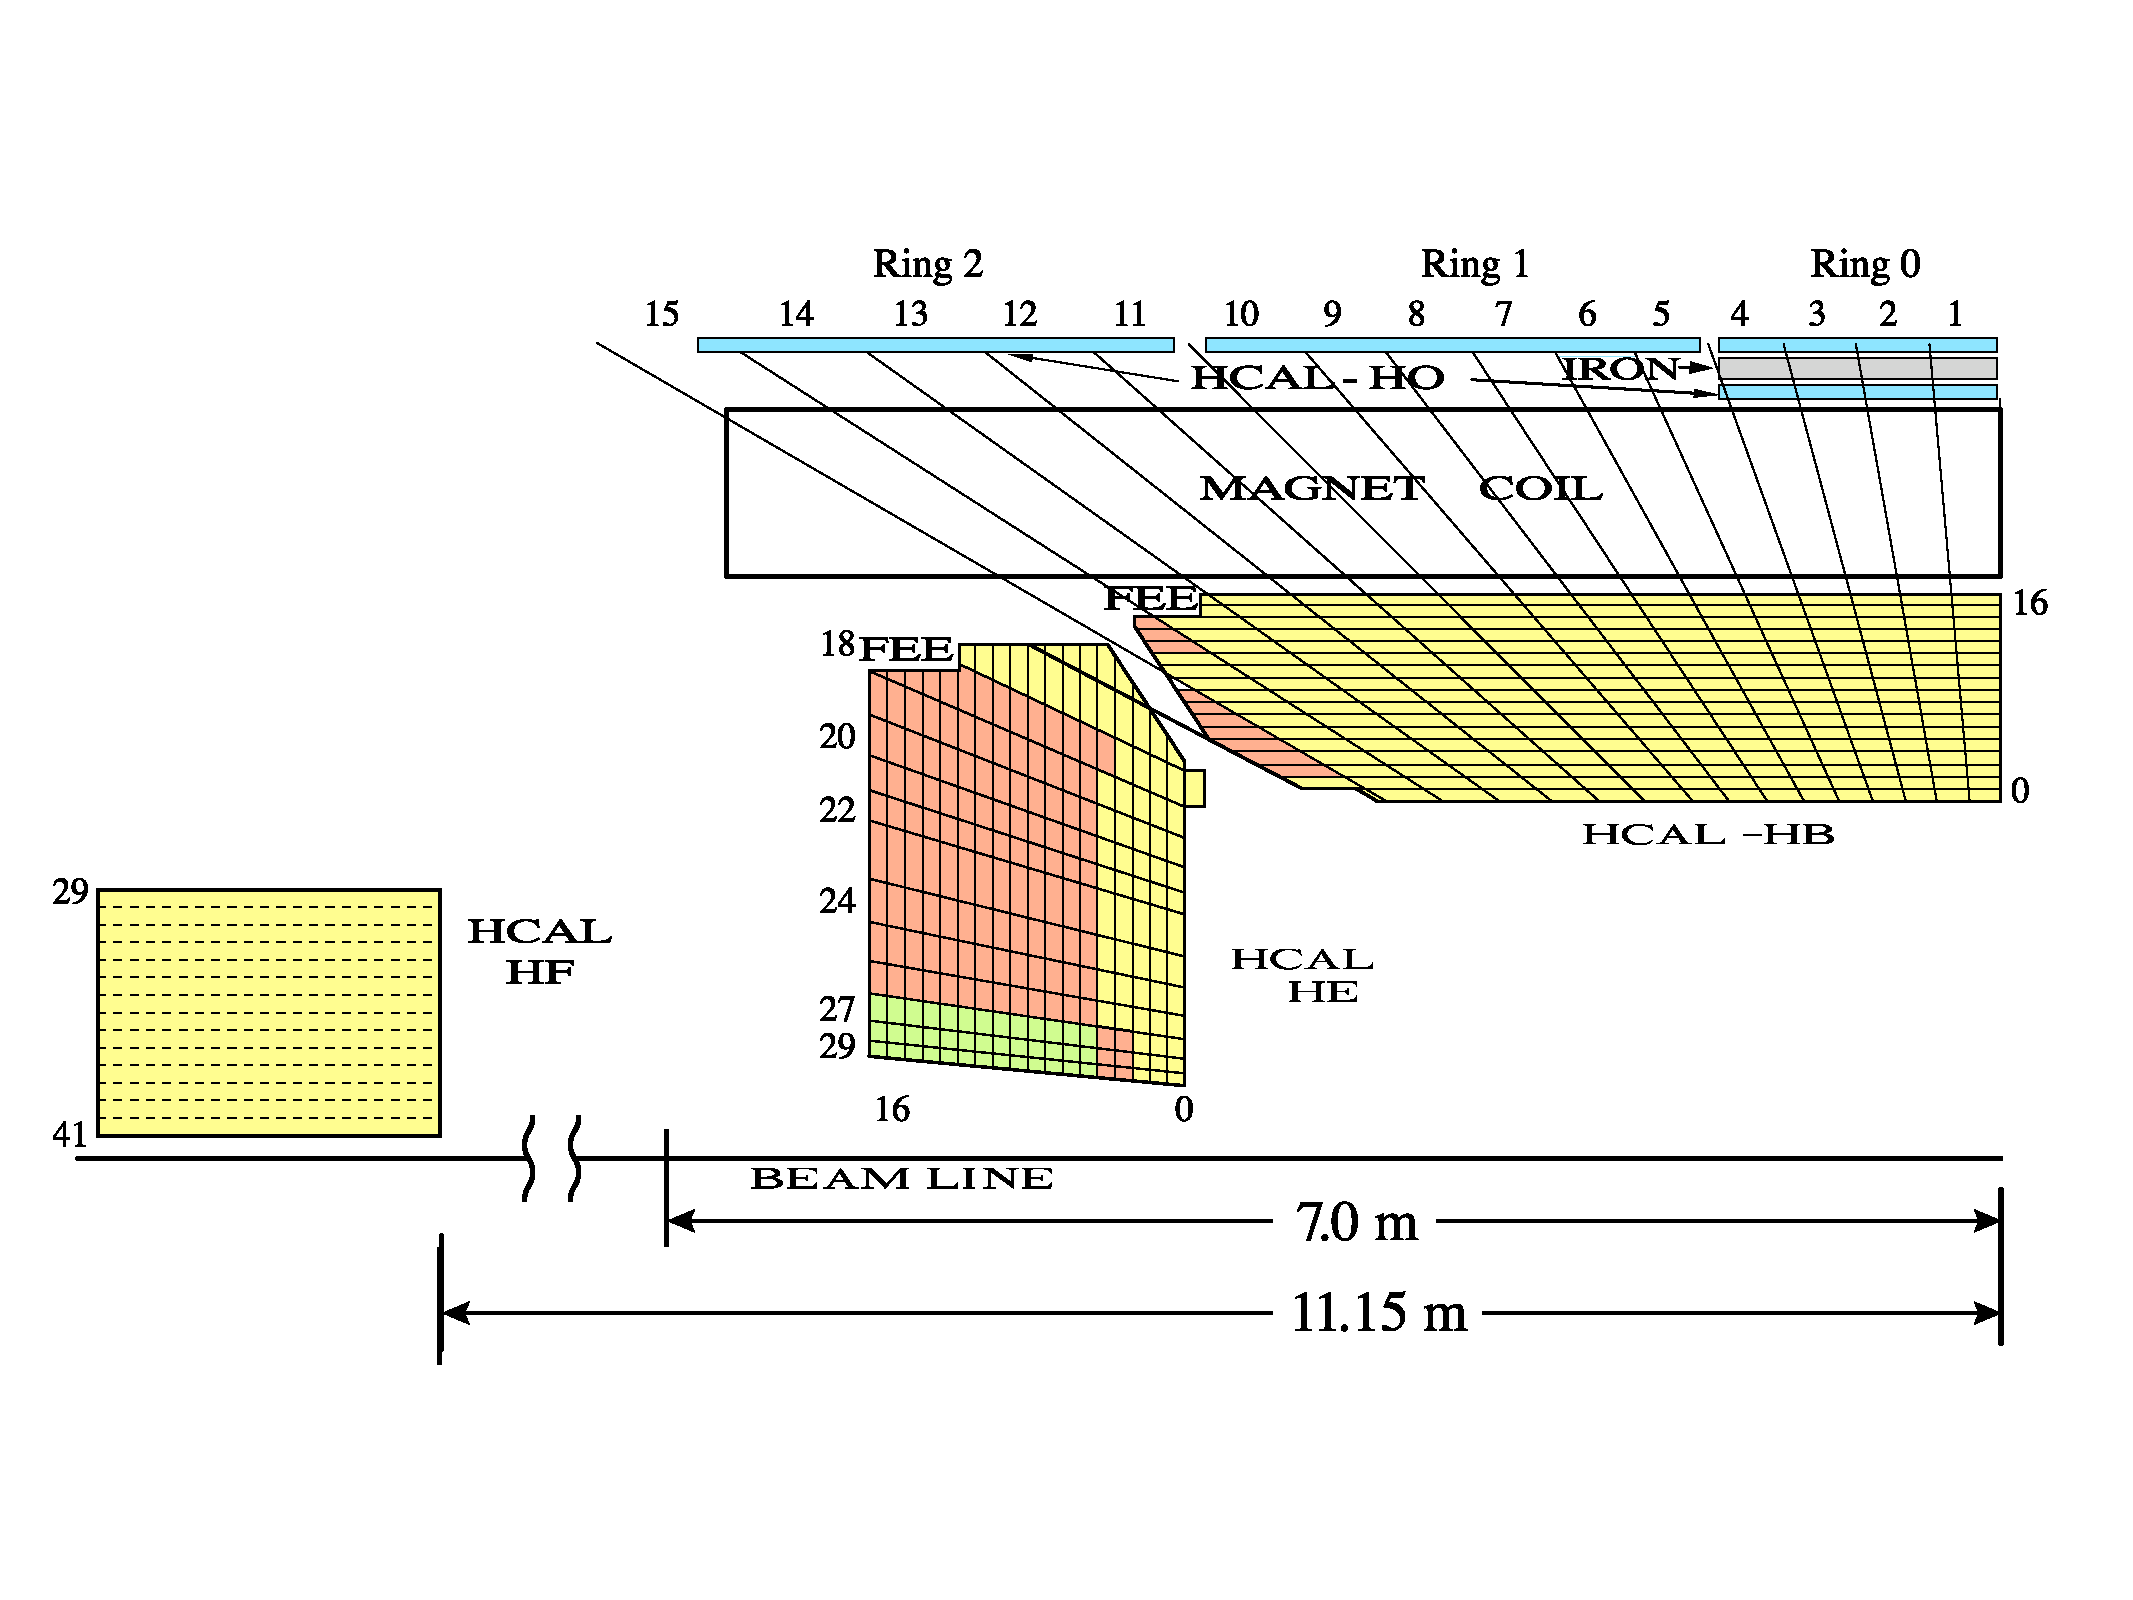
\includegraphics[width=0.99\textwidth]{CMS_DetectorFigures/HCAL_Layout.pdf}
\caption{The CMS HCAL layout.\label{fig:HCAL_Layout}}
\end{figure}

The hadronic energy resolution for the barrel HCAL and ECAL
combination was measured in beam test using pions and protons and
found to be:

\begin{equation}
\label{eq:hcal_res}
\frac{\sigma_{E}}{E} = \frac{0.847\pm0.016\GeV^{\frac{1}{2}}}{\sqrt{E
    (\GeV)}} \oplus 0.074\pm 0.008.
\end{equation}
The energy resolution in the endcaps is similar to that of the barrel.

The following passages are aimed to give a more detailed description
of the four HCAL subsystems.

\subsection{The Barrel Hadronic Calorimeter}
The HB is a sampling calorimeter made of brass absorber and plastic
scintillator as the active medium. The whole EB is build out of two
identical cylindrical structures, each of which is composed of 18
brass wedges. The pseudorapidity coverage of the HB reaches
approximately $|\eta| = 1.4$ while the $\phi$ covarage is
360$^{\circ}$. The segmentation of the HB is provided by the plastic
scintillator tiles inserted in the layers of the brass wedges, the later
are segmented into four $\phi$ sector, while there are 16 scintillator
tiles along the $\eta$ direction, thus providing the HB with an
equivalent segmentation of 0.087$\times$0.087 in $\eta$, $\phi$. Each
wedge calorimeter is composed of 16 layers of absorber and 17 layers of
plastic scintillator, the intermediate layer are made of brass
absorber and 3 mm plastic scintillator while the first and last layers
are made of stainless steel  and thicker 9 mm plastic scintillator
tiles. The very first layer is scintillator in order to detect showers
developed in the electromagnetic calorimeter
material. Figure~\ref{fig:HCALwedge} shows an schematic of a HB
wedge. The 16 scintillator tiles of each layer are laid in a tray in
order to facilitate their insertion and removal. Each tile's
scintillating light is collected by a green double-cladded
wavelength-shinting (WLS) fibers from Kuraray (Y-11) placed in groove
in the scintillator. Upon exiting the scintillating tile, each WLS is
splice into a clear fiber which subsequently ends in an optical
connector at the back of the tray. At this point, optical cables
take the light from the clear fiber into a 19 pixel hybrid photodiode
(HPD), which is designed to work inside the 3.8 T magnetic field. The
total interaction lengths ($\lambda_{I}$) of the HB varies with
pseudoparidity, there are 5.8 $\lambda_{I}$ at $\eta = 0$, increasing
up to 10.6 $\lambda_{I}$ at $|\eta| = 1.3$.
The finalized HB is shown in Figure~\ref{fig:hcal}.
\begin{figure}
 \centering
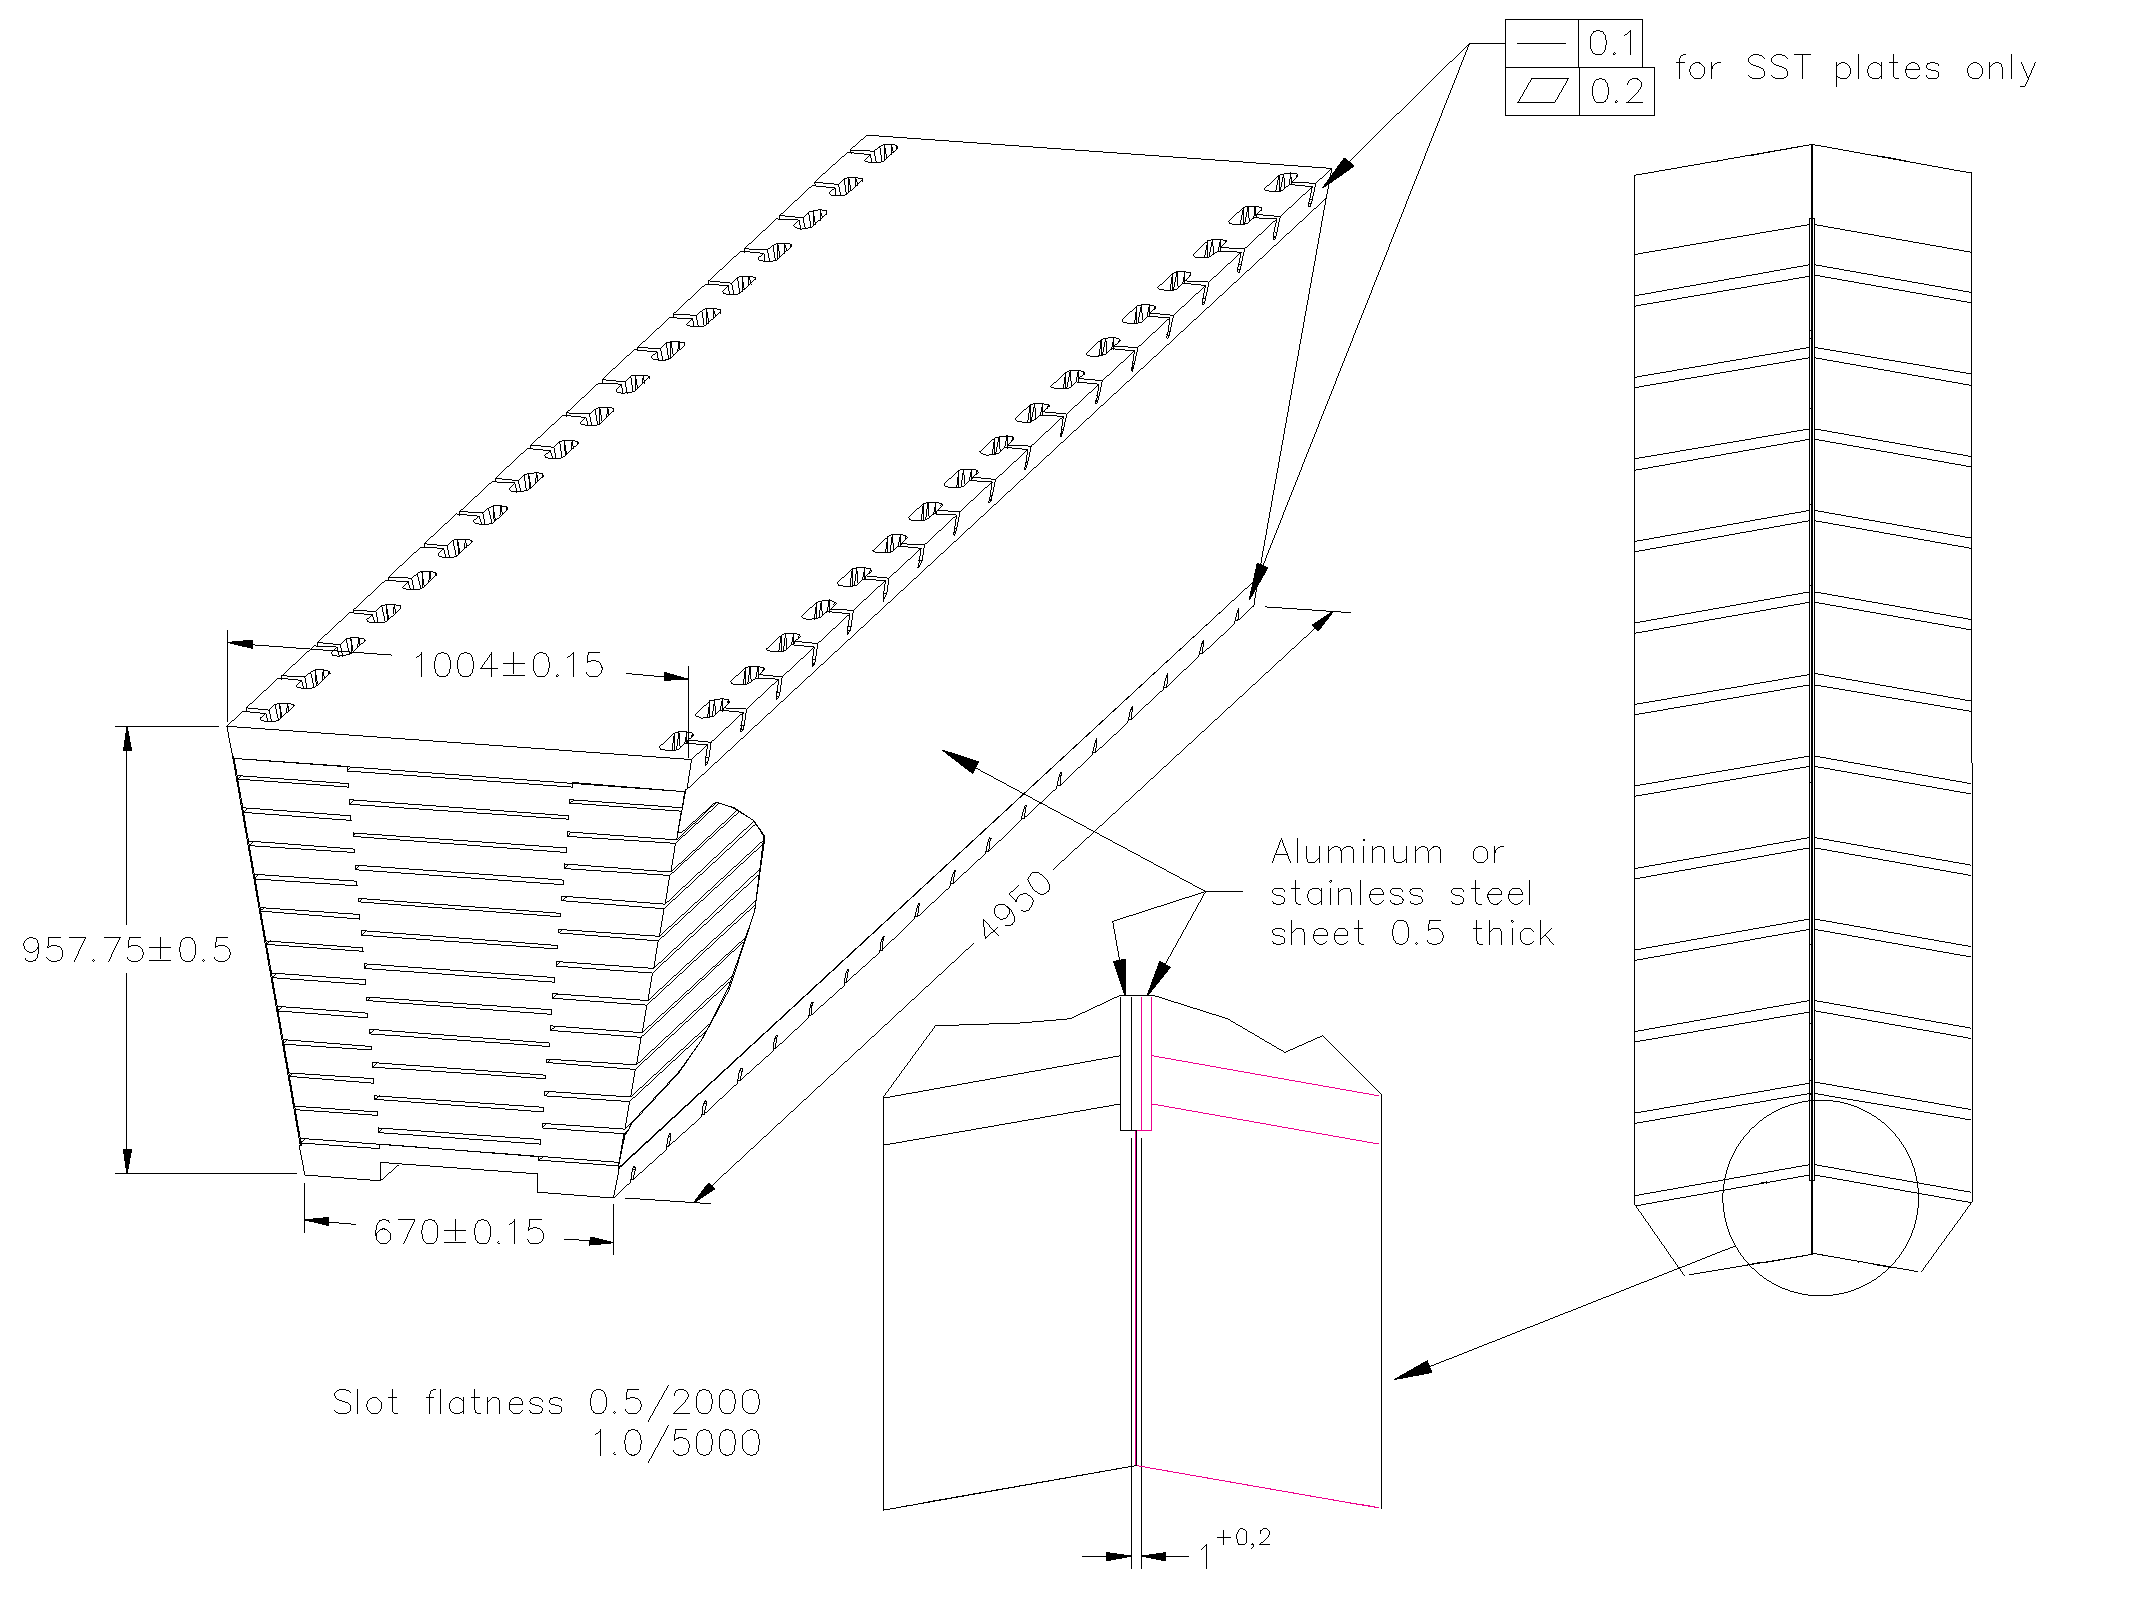
\includegraphics[width=0.99\textwidth]{CMS_DetectorFigures/HCAL_Wedge.pdf}
\caption{An schematic drawn of one of the wedges of the CMS HB.\label{fig:HCALwedge}}
\end{figure}
\begin{figure}
 \centering
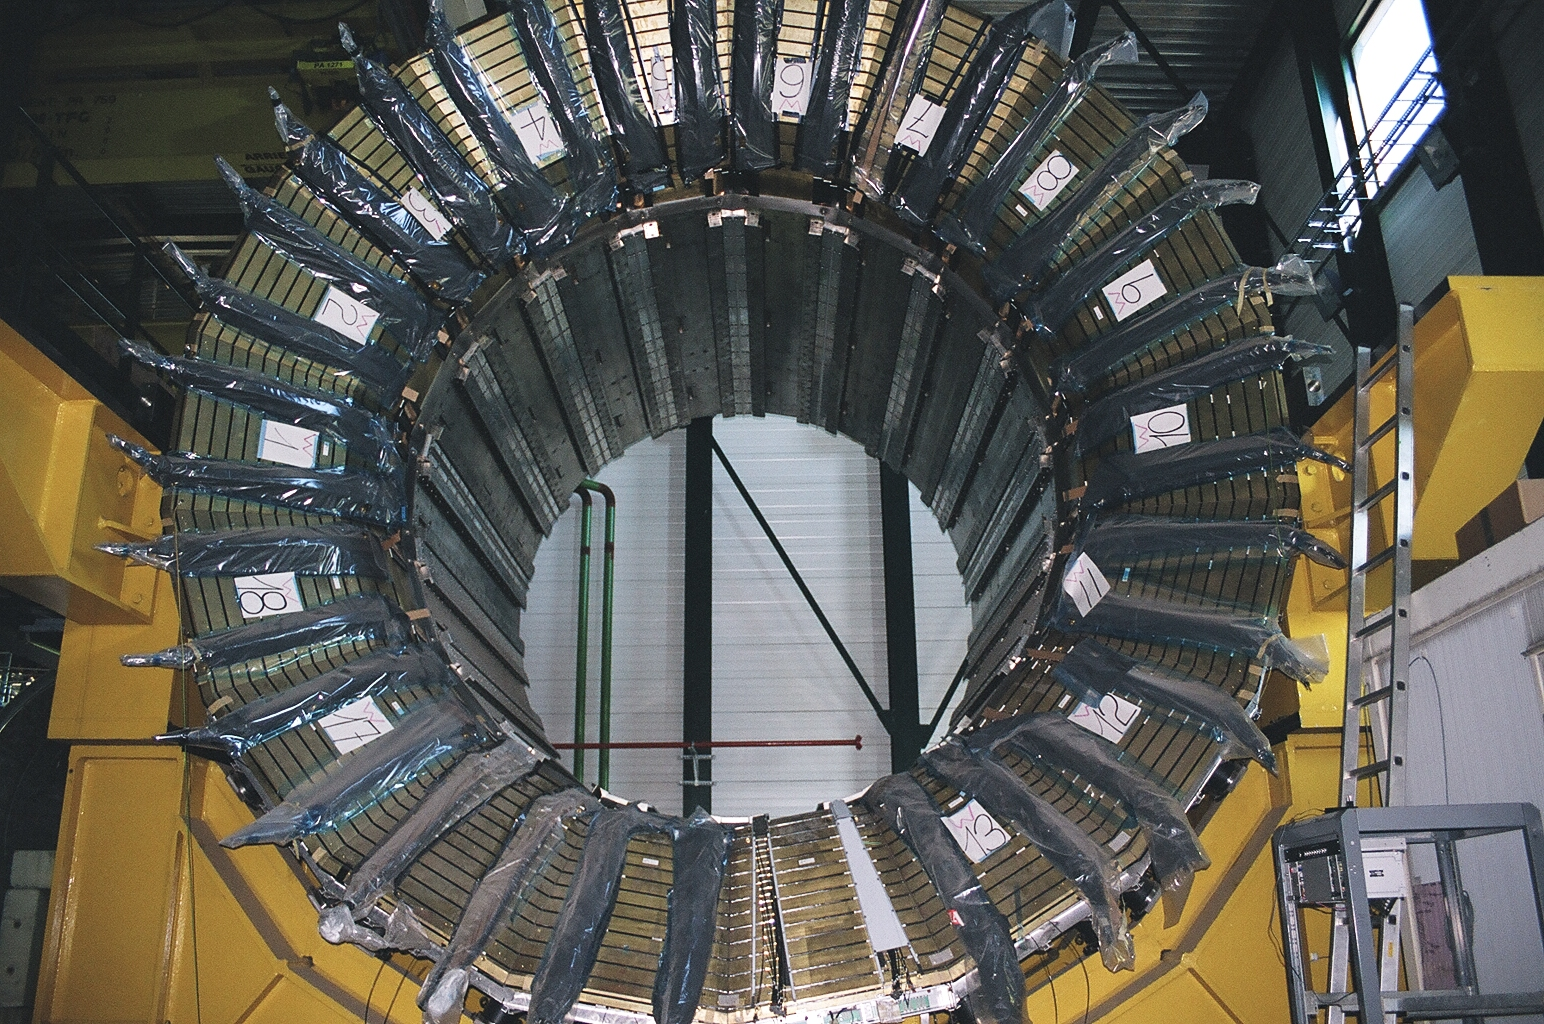
\includegraphics[width=0.99\textwidth]{CMS_DetectorFigures/hcal-HB.jpg}
\caption{A photograph of the finalized CMS HB.\label{fig:hcal}}
\end{figure}
\subsection{The Endcap Hadronic Calorimeter}
The HE is a brass/platic-scintillator sampling calorimeter that extend
the pseudorapidity coverage from $1.3 < |\eta| < 3$. It is composed of
79-mm-thick brass plates with 9 mm gaps to accomodate the
scintillator. The total material, including the crystals in the EE, is
about 10 $\lambda_{I}$. There are 18 layers -- along the $z$-direction
-- of plastic scintillators, the first layer, right after the EE, is
9-mm-thick, while the rest are 3-mm-thick. The scintillators are
segmented in the radial direction and their light is collected by
embedded WLS fiber. The scintillator tiles and the WLS are laid in
trays with a trapezoidal geometry. Figure~\ref{fig:HEtiles} shows an
schematic of the trays. The WLS are spliced to clear fibers which are
susequently terminated in an optical connector. Optical cables
transport the light from the optical connector the HPDs, which, as
mentioned earlier, could operate in the presense of a magnetic
field. This design results in a granularity of 0.087$\times$0.087
($\eta\times\phi$) for $|\eta| < 1.6$ and 0.17$\times$0.17 for $|\eta|
> 1.6$. Figure~\ref{fig:HE} shows one partially finalized HE, where
only some of the scintillator trays have been inserted.

\begin{figure}
 \centering
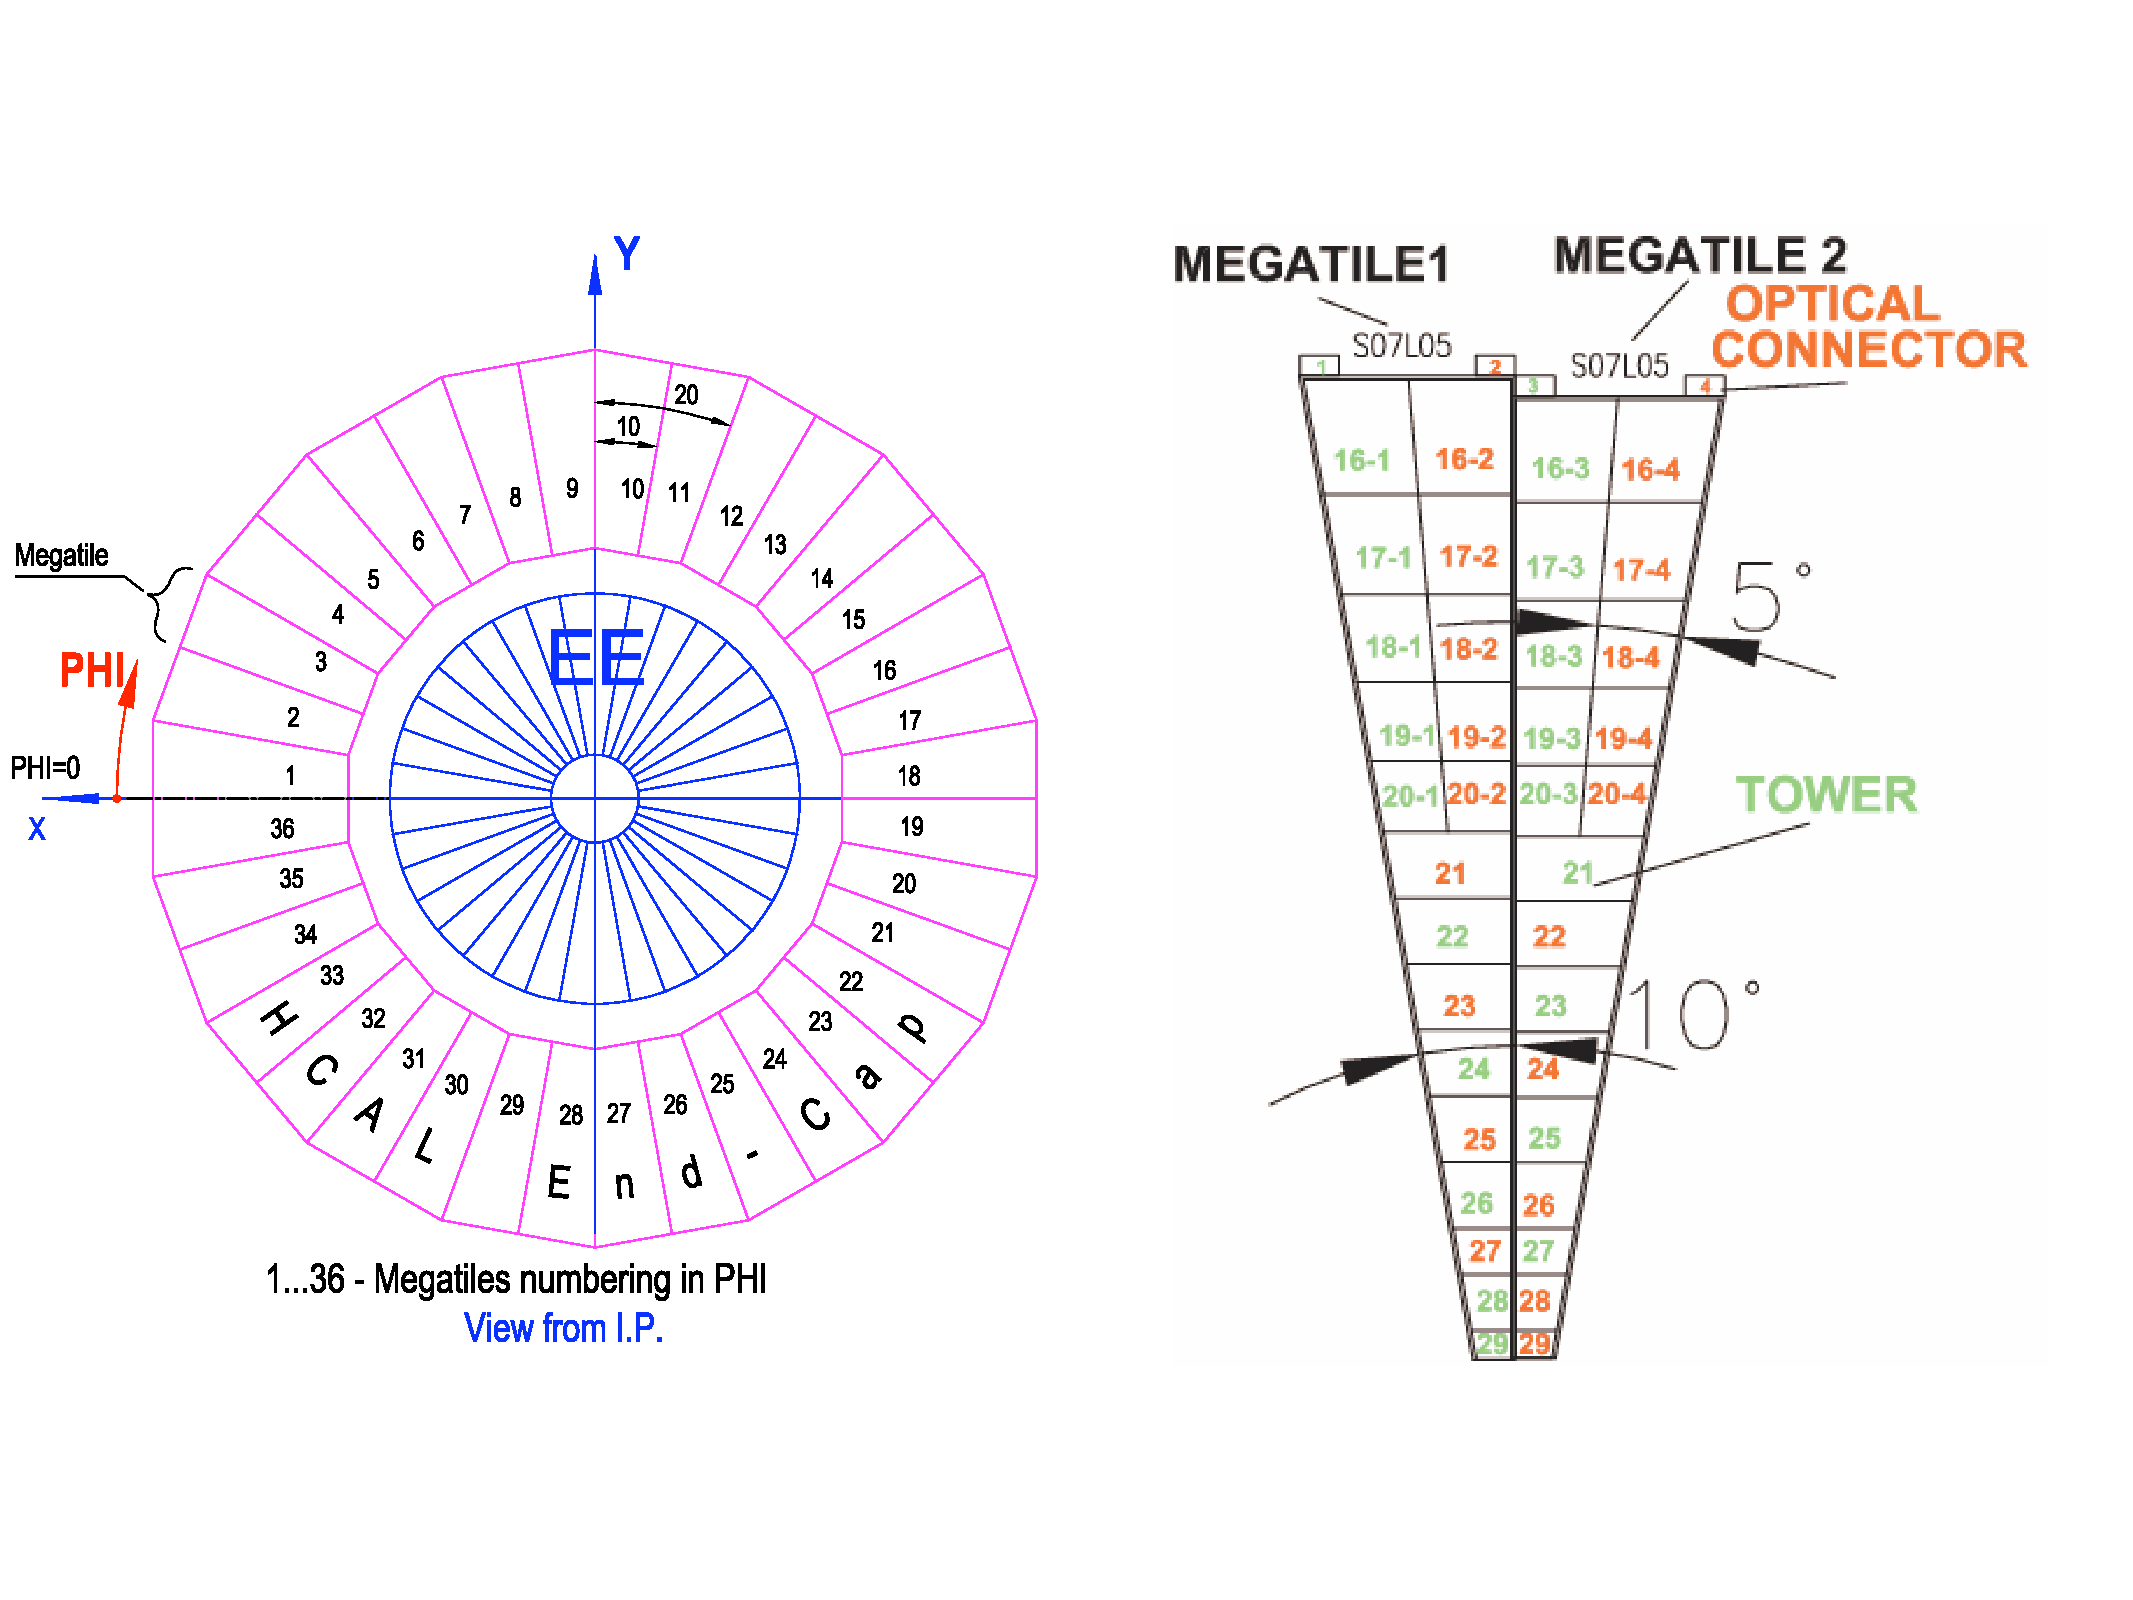
\includegraphics[width=0.99\textwidth]{CMS_DetectorFigures/hca_tile.pdf}
\caption{An schematic of the HE geometry in the $\phi$ direction is
  presented in the left panel. The configuration of two adjacent
  scintillator trays is presented in the right panel.\label{fig:HEtiles}}
\end{figure}
\begin{figure}
 \centering
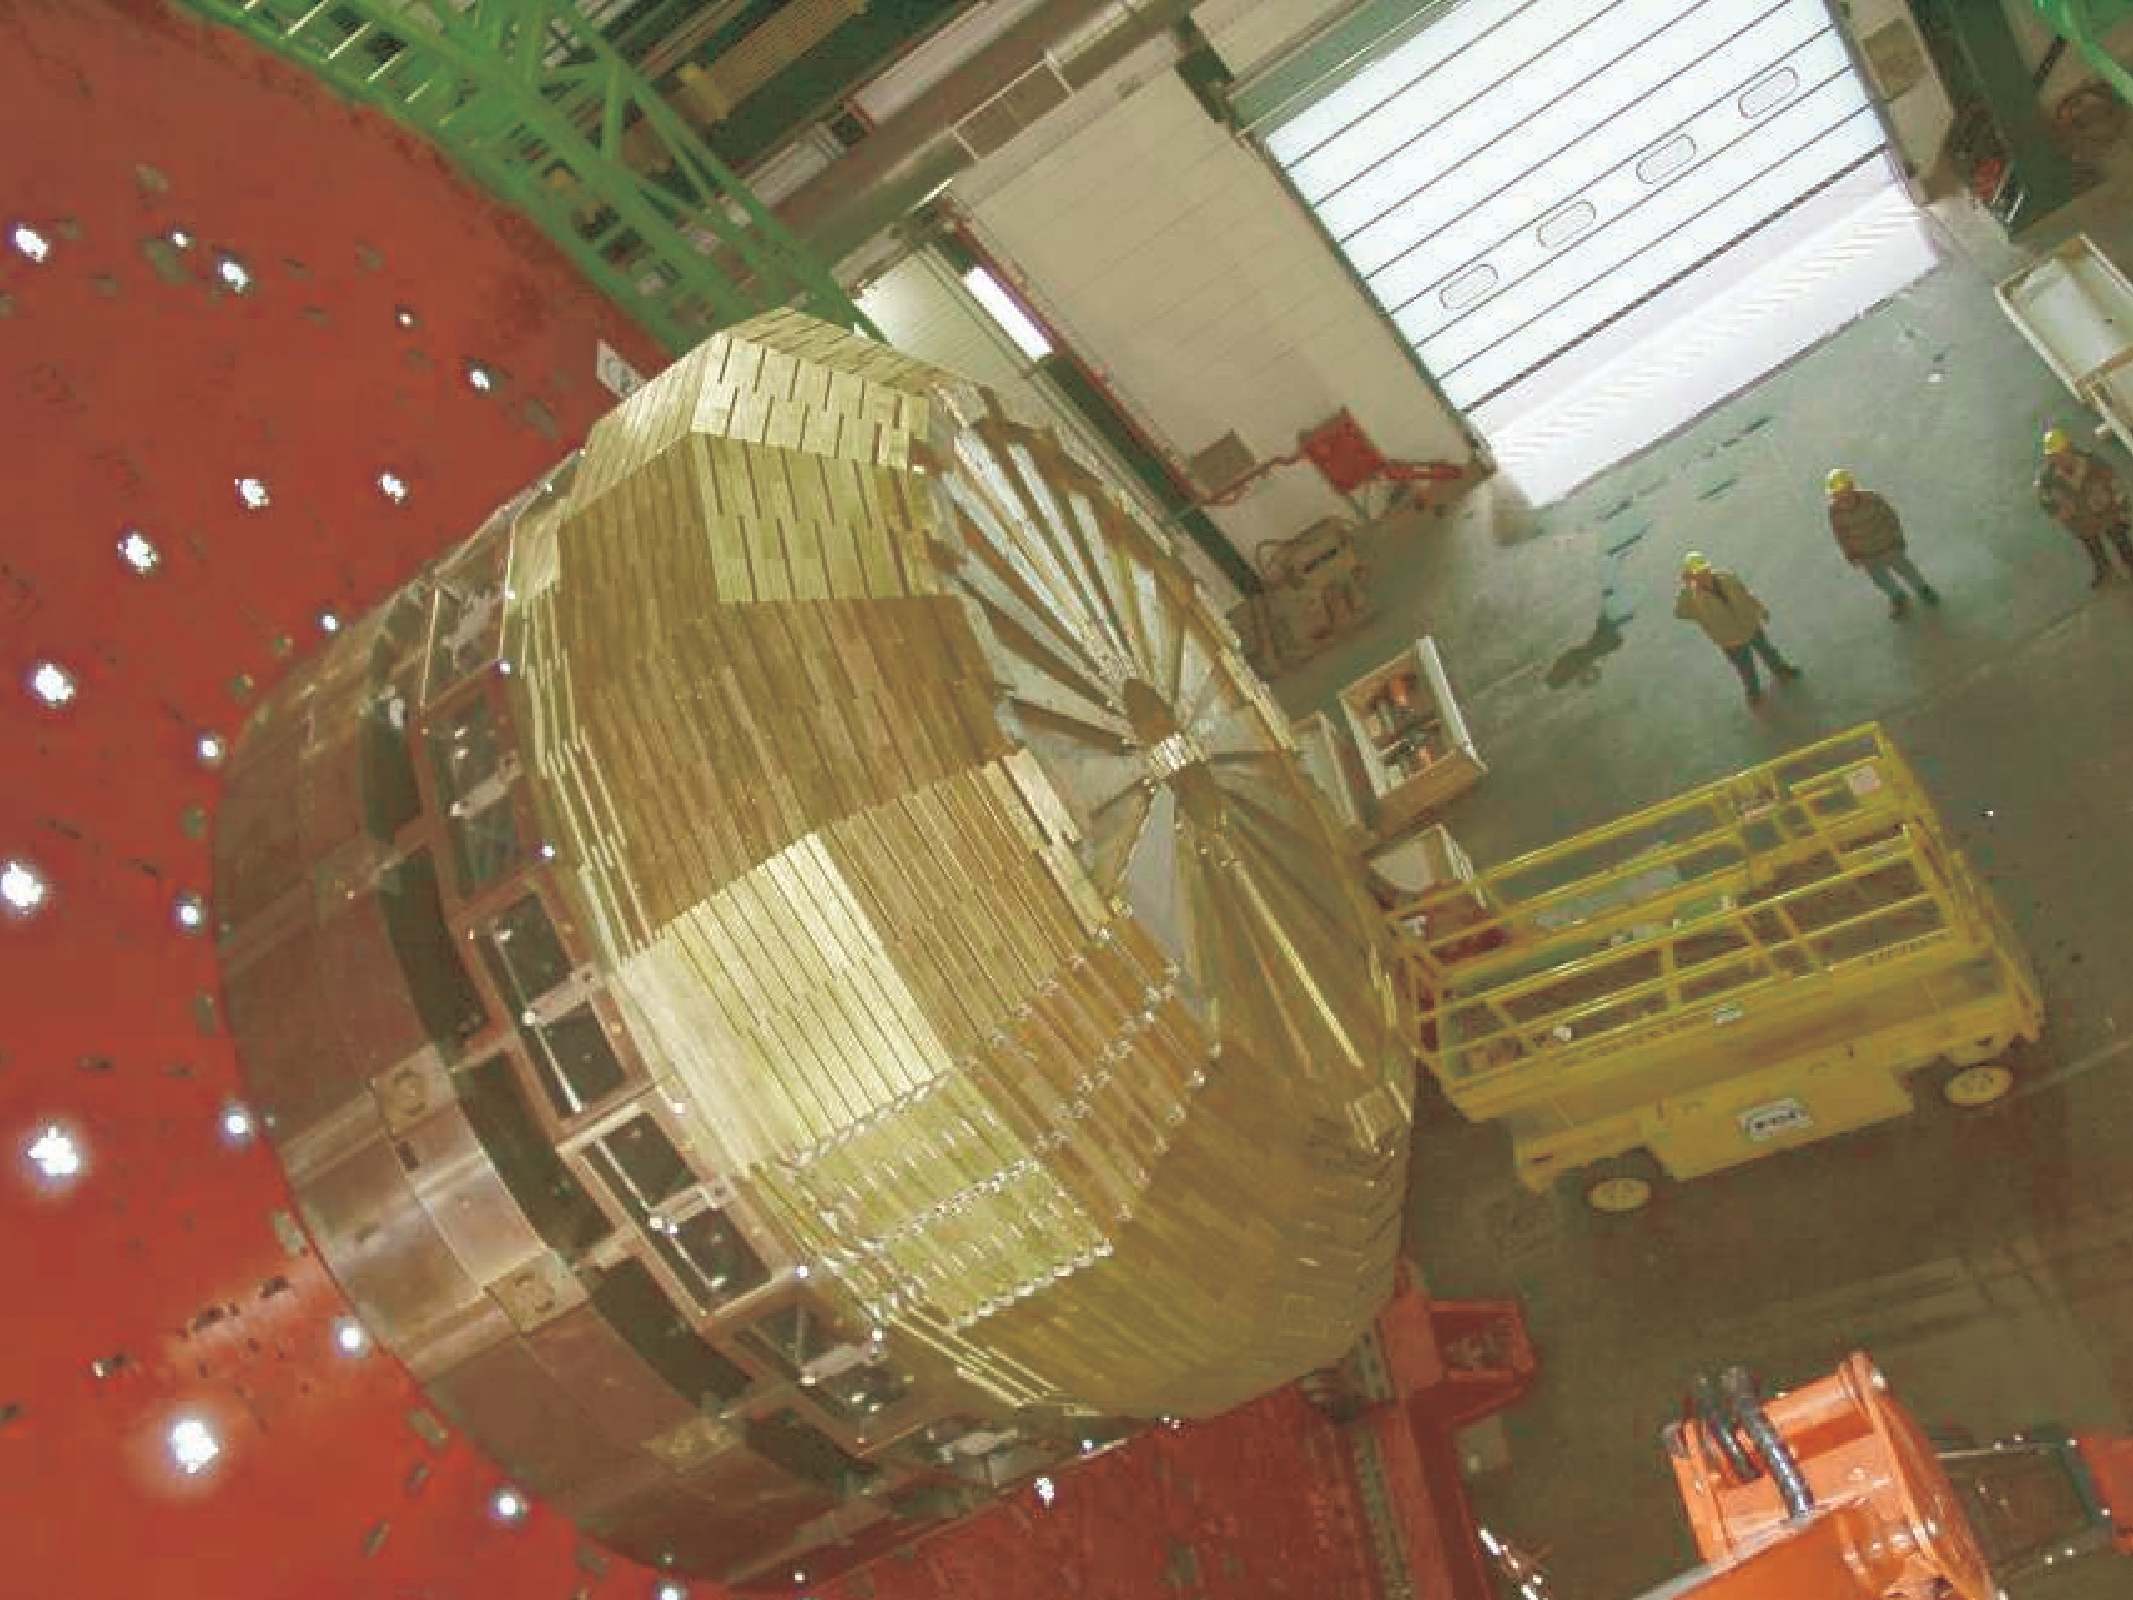
\includegraphics[width=0.99\textwidth]{CMS_DetectorFigures/hcal_HE.pdf}
\caption{A photograph of the one partially finalized CMS HE.\label{fig:HE}}
\end{figure}

\subsection{The Outer Hadronic Calorimeter}
\subsection{The Forward Hadronic Calorimeter}
\section{The Superconducting Solenoid}
\section{The Muon Chambers}
\section{Physics Object Reconstruction}
\subsection{Muon Identification}
\subsection{Electron and Photon Identification}
\subsection{Jet Identification}
\subsection{Missing Energy Reconstruction}
\section{Introduction}
The existence of dark matter (DM) in the universe, originally proposed~\cite{Zwicky:1937zza} to
reconcile observations of the Coma galaxy cluster with
the prediction from the virial theorem, is
commonly accepted as the explanation of many experimental
phenomena in astrophysics and cosmology, such as galaxy rotation
curves~\cite{vandeHulst,Rubin:1980zd}, large structure
formation~\cite{White:1987yr,Carlberg:1989yr,Springel:2005nw}, and the
observed
spectrum~\cite{Smoot:1992td,deBernardis:2000gy,Spergel:2006hy,Ade:2013zuv}
of the cosmic microwave background~\cite{Bardeen:1985tr}. A global fit to
cosmological data in the $\Lambda$CDM model (also known as
the standard model of cosmology)~\cite{Cen:2000xv} suggests that
approximately 85\% of the mass of the universe is attributable to
DM~\cite{Ade:2013zuv}. To accommodate these observations and the
dynamics of colliding galaxy clusters~\cite{Clowe:2006eq}, it has been
hypothesized that DM is made mostly of weakly
interacting massive particles
(WIMPs), sufficiently massive to be in nonrelativistic motion
following their decoupling from the hot particle plasma in the early
stages of the expansion of the universe.

While the standard model (SM) of particle physics does not include a
viable DM candidate, several models of physics beyond the SM, e.g.,
supersymmetry (SUSY)~\cite{Ramond,Golfand,Volkov,Wess,Fayet} with $R$-parity
conservation, can accommodate the existence of WIMPs. In these models,
pairs of DM particles can be produced in proton-proton (pp) collisions at
the CERN LHC. Dark matter particles would not leave a detectable signal in
a particle detector. When produced in association with high-energy
quarks or gluons, they could provide event topologies with
jets and a transverse momentum (\pt) imbalance ($\ptvecmiss$). The magnitude of $\ptvecmiss$ is referred to as missing transverse energy ($\ETm$).
The ATLAS and CMS collaborations have reported searches for events with one
high-\pt jet and large $\ETm$~\cite{Aad:2011xw,Chatrchyan:2012me}, which are sensitive to such topologies.
In this paper, we refer to these studies as monojet searches. Complementary studies of events with
high-\pt photons~\cite{Khachatryan:2014rwa,Aad:2014tda}; \PW,
\cPZ,~or
Higgs~bosons~\cite{Aad:2013oja,Aad:2014vka,Aad:2015dva,Aad:2015yga};
b jets~\cite{Aad:2014vea} and top quarks~\cite{Aad:2014vea,CMS:b2g12-022,CMS:semilepTop}; and leptons~\cite{ATLAS:2014wra,Khachatryan:2014tva}
have also been performed.

This paper describes a search for dark matter particles $\chi$ in events with at least two jets of comparable transverse momenta
and sizable $\ETm$. The search is based
on the razor variables $\MR$ and $\RR^2$~\cite{rogan,razor2010}.  Given a
dijet event, these variables are computed from the two jet momenta $\vv{p}^{j_1}$ and
$\vv{p}^{j_2}$, according to the following
definition:
 \begin{align}
 \begin{split}
 \MR  & =
 \sqrt{
  (\abs{\vv{p}^{j_1}}+\abs{\vv{p}^{j_{2}})^2 -
  (p^{j_1}_{z}+p^{j_2}_{z})^2}},
\\
 \mathrm{R}  & =   \frac{M^{\RR}_\mathrm{T}}{\MR},
\label{eq:razor}
\end{split}\\
\intertext{with}
 \label{eq:MTR}
 M^{\RR}_\mathrm{T}  &=   \sqrt{ \frac{\ETm(\pt^{j_1}+\pt^{j_2}) -
   \ptvecmiss {\cdot}
   (\vv{p}_{\mathrm{T}}^{\,j_1}+\vv{p}_{\mathrm{T}}^{j_2})}{2}}.
\end{align}

In the context of SUSY, $\MR$ provides an estimate of the
underlying mass scale of the event, and quantity $M^{\RR}_\mathrm{T}$ is a transverse
observable that includes information about the
topology of the event. The variable $\RR^2$ is designed to reduce QCD
multijet background; it is correlated with the angle
between the two jets, where co-linear jets have large $\RR^2$ while back-to-back jets have small $\RR^2$.
These variables have been used to study the production of non-interacting
particles in cascade decays of heavier partners, such as squarks and
gluinos in SUSY models with $R$-parity
conservation~\cite{Chatrchyan:2014goa,Razor8TeV}. The sensitivity of
these variables to direct DM production was suggested in
Ref.~\cite{Fox:2012ee}, where it was pointed out that the dijet event
topology provides good discrimination against background processes,
with a looser event selection than that applied in the monojet searches.
Sensitivity to DM production is most enhanced for large values of
$\RR^2$, while categorizing events based on the value of $\MR$
improves signal to background discrimination and yields significantly improved
search sensitivity to a broader and more inclusive class of DM models. 
The resulting sensitivity is expected to be 
comparable to that of monojet searches~\cite{Fox:2012ee,Papucci:2014iwa}. This
strategy also offers the possibility to search for DM particles that
couple preferentially to b quarks~\cite{Agrawal:2014una}, as proposed
to accommodate the observed excess of photons with energies between
1 and 4\GeV in the gamma ray spectrum of the galactic center data collected by the Fermi-LAT gamma-ray space
telescope~\cite{Hooper:2010mq}. The results are interpreted using an
effective field theory approach and the Feynman diagrams for DM pair production are shown in Fig.~\ref{fig:DMdiamgrams}.

\begin{figure}
 \centering
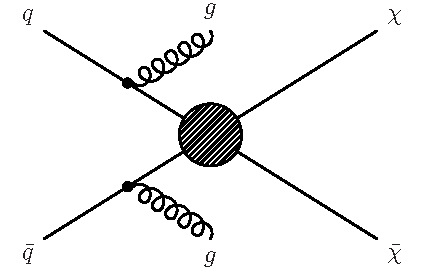
\includegraphics[width=0.35\textwidth]{Diagrams/RazorDMdiagram.pdf}
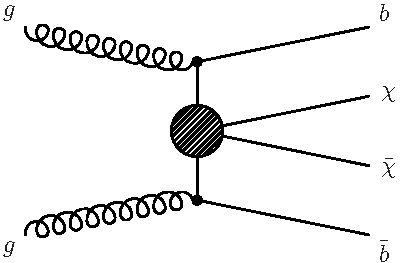
\includegraphics[width=0.35\textwidth]{Diagrams/dmdm_bbar.pdf}
 \caption{Feynman diagrams for the pair production of DM particles
   corresponding to an effective field theory using a vector or
   axial-vector operator (left), and a scalar operator (right).\label{fig:DMdiamgrams}}
\end{figure}


Unlike the SUSY razor searches~\cite{Razor8TeV,razor2010}, which focus on events with large
values of $\MR$, this study also considers events with small values
of $\MR$, using $\RR^2$ to discriminate
between signal and background, in a kinematic region ($\RR^2 >
0.5$) excluded by the baseline selection of Refs.~\cite{Razor8TeV,razor2010}.

A data sample corresponding to an integrated luminosity of
18.8\fbinv of pp collisions at a center-of-mass energy of 8\TeV  was collected by the CMS experiment
 with a trigger based on a
loose selection on $\MR$ and $\RR^2$. This and other
special triggers were operated in 2012 to record events at a rate
higher than the CMS computing system could process during data
taking. The events from these triggers were stored on tape and their
reconstruction was delayed until 2013, to profit from the larger availability of processing resources during the LHC shutdown.
These data, referred to as ``parked data''~\cite{CMS-DP-2012-022},
enabled the exploration of events with small $\MR$
values, thereby enhancing the sensitivity to direct DM production.

This paper is organized as follows:  section~\ref{sec:sample}
describes the data and simulated samples of events used in the
analysis. Sections~\ref{sec:selection} and~\ref{sec:sampleDef} discuss
the event selections and categorization, respectively. The
estimation of the background is described in Section~\ref{sec:bkg}.
The systematic uncertainties are discussed in Section~\ref{sec:sys},
while Section~\ref{sec:interpretation} presents the results and the
implications for several models of DM production. A summary is given in Section~\ref{sec:conclusions}.

% \section{The CMS detector}\label{cmsdetector}

% The central feature of the CMS apparatus is a superconducting solenoid
% of 6\unit{m} internal diameter, providing a magnetic field of
% 3.8\unit{T}. Within the solenoid volume are a silicon
% pixel and strip tracker, a lead tungstate crystal electromagnetic
% calorimeter (ECAL), and a brass and scintillator hadron calorimeter
% (HCAL), each composed of a barrel and two endcap sections.
% When combining information from the entire detector, the jet energy resolution amounts typically to 15\% at 10\GeV, 8\% at 100\GeV, and 4\% at 1\TeV~\cite{Chatrchyan:2013dga}. Muons are
% measured in gas-ionization detectors embedded in the steel flux-return
% yoke outside the solenoid. Forward calorimeters extend the
% pseudorapidity ($\eta$)~\cite{Chatrchyan:2008zzk} coverage provided by the
% barrel and endcap detectors. The first level (L1) of the CMS trigger system, composed of custom
% hardware processors, uses information from the calorimeters and muon
% detectors to select the most interesting events in a fixed time
% interval of less than 4\mus. The high-level trigger (HLT) processor
% farm further decreases the event rate from around 100\unit{kHz} to
% around 400\unit{Hz}, before data storage. A more
% detailed description of the CMS detector, together with a definition
% of the coordinate system used and the basic kinematic variables, can
% be found in Ref.~\cite{Chatrchyan:2008zzk}.

\section{Data set and simulated samples}
\label{sec:sample}
The analysis is performed on events with two jets reconstructed at L1
in the central part of the detector ($\abs{\eta}< 3.0$). The L1 jet
triggers are based on the sums of
transverse energy in regions $\Delta\eta\times\Delta\phi$
approximately 1.05$\times$1.05 in
size~\cite{Chatrchyan:2008zzk} (where $\phi$ is the azimuthal angle in the plane transverse to the LHC beams.).
At the HLT, energy deposits in ECAL and HCAL are clustered into jets and the
razor variables $\RR^2$ and $\MR$ are computed. In the
HLT, jets are defined using the {\FASTJET}~\cite{fastjet}
implementation of the anti-\kt~\cite{antikt} algorithm, with
a distance parameter equal to 0.5. Events with at least two jets
with $\pt>64$\GeV are
considered. Events are selected with $\RR^2> 0.09$ and
$\RR^2 \times \MR > 45$\GeV. This selection
rejects the majority of the background, which tends to have low $\RR^2$ and low
$\MR$ values, while keeping the events in the signal-sensitive
regions of the ($\MR$, $\RR^2$) plane.
The trigger efficiency, measured using a pre-scaled trigger with very loose thresholds, is
shown in Table~\ref{tab:Trigger}.  The requirements described above correspond to the least stringent event selection, given the constraints on the maximum acceptable rate.

\begin{table}[htb]
\centering
  \topcaption{\label{tab:Trigger}Measured trigger efficiency for different
    $\MR$ regions. The selection $\RR^2 > 0.35$ is applied. The uncertainty
    shown represents the statistical uncertainty in the measured efficiency.
}
\begin{tabular}{cccc}
  \hline
  $\MR$ region (\GeVns{}) & 200--300 &  300--400 &
  400--3500 \rule{0pt}{2.3ex} \rule[-1.2ex]{0pt}{0pt}\\
  \hline
  Trigger efficiency (\%) & $91.1\pm ^{1.5}_{1.7}$ &
  $90.7\pm^{2.3}_{2.9}$ & $94.4 \pm ^{2.4}_{3.6}$ \rule{0pt}{2.3ex} \rule[-1.2ex]{0pt}{0pt}\\
  \hline
\end{tabular}
\end{table}

Monte Carlo (MC) simulated signal and background samples are generated with the
leading order matrix element generator {\MADGRAPH
  v5.1.3}~\cite{Alwall:2011uj,Alwall:2014hca} and the CTEQ6L parton
distribution function set~\cite{Pumplin:2002vw}. The generation
includes the \PYTHIA 6.4.26~\cite{Sjostrand:2006za} Z2* tune, which is
derived from Z1 tune~\cite{Field:2010bc} based on the CTEQ5L set.
Parton shower and hadronization effects are included by matching the generated events to \PYTHIA, using the MLM matching algorithm~\cite{Hoche:2006ph}.
The events are processed with a \GEANTfour~\cite{G4} description of the CMS apparatus to include
detector effects. The simulation samples for SM
background processes are scaled to the
integrated luminosity of the data sample (18.8\fbinv), using
calculations of the inclusive production cross sections at the next-to-next-to-leading
order (NNLO) in the perturbative QCD
expansion~\cite{WatNNLO,ZatNNLO,TTbaratNNLO}.
 The signal processes corresponding to pair production of DM particles
 are simulated with up to two additional partons with $\pt>80$\GeV.

\section{Event selection}\label{sec:selection}

Events are selected with at least one reconstructed
interaction vertex within $\abs{z}<24$\cm. If more than one vertex is
found, the one with the highest sum of the associated track momenta squared is used as the
interaction point for event reconstruction. Events containing
calorimeter noise, or large missing transverse momentum
due to beam halo and instrumental effects (such as jets near
non-functioning channels in the ECAL) are removed from the analysis~\cite{MET_8TeV}.

A particle-flow (PF) algorithm~\cite{PF1,CMS-PAS-PFT-10-001} is used to reconstruct
and identify individual particles with an optimized combination of
information from the various elements of the CMS detector. The energy
of photons is directly obtained from the ECAL measurement, corrected
for zero-suppression effects. The energy of electrons is determined
from a combination of the electron momentum at the primary interaction
vertex as measured by the tracker, the energy of the corresponding
ECAL cluster, and the energy sum of all bremsstrahlung photons (or emissions)
spatially compatible with originating from the electron track. The
energy of muons is obtained from the curvature of the associated
track. The energy of charged hadrons is determined from a combination
of their momentum measured in the tracker and the matching ECAL and
HCAL energy deposits, corrected for zero-suppression effects and for
the response function of the calorimeters to hadronic
showers. Finally, the energy of neutral hadrons is obtained from the
corresponding corrected ECAL and HCAL energies. Contamination of the
energy determinations from other pp collisions is mitigated by
discarding the charged PF candidates incompatible with originating from the main vertex.  Additional
energy from neutral particles is subtracted on average when computing
lepton (electron or muon) isolation and jet energy. This contribution is estimated as the
per-event energy deposit per unit area, in the cone $\Delta R = \sqrt{\smash[b]{(\Delta
  \eta)^2+(\Delta\phi)^2}}=0.3$, times the considered jet size or
isolation cone area.

Electrons (muons) are required to have $\pt>15$\GeV and  $\abs{\eta}<2.5$
(2.4). In order to reduce the
background from hadrons misidentified as leptons, additional
requirements based on the
quality of track reconstruction and isolation are applied. Lepton isolation is
defined as the scalar \pt sum of all PF candidates other than the
lepton itself, within a cone of size $\Delta R = 0.3$, and normalized to the lepton \pt. A
candidate is identified as a lepton if the isolation variable is found to be smaller than 15\%.
For electrons~\cite{ElectronsCMS}, a characteristic of the shower
shape of the energy deposit in the ECAL (the shower width in the
$\eta$ direction) is used to further reduce the contamination from hadrons.
PF candidates with $\pt > 10$\GeV that are not consistent with muons and satisfy the same isolation
requirements as those used for electrons are also identified to increase the 
lepton selection efficiency as well as to identify single-prong tau decays. 


Jets are formed by clustering the PF candidates, using the anti-\kt algorithm with distance
parameter 0.5. Jet momentum is determined as the vectorial sum of all
particle momenta in the jet, and is found from simulation to be within
5\% to 10\% of the generated hadron level jet momentum over the whole \pt spectrum and
detector acceptance.
 Jet energy corrections
are derived from simulation, and are confirmed with in situ
measurements of the energy balance in dijet and photon+jet events.
Additional selection criteria are applied to each event to remove
spurious jet-like features originating from isolated noise patterns in certain HCAL regions.
We select events containing at least two jets with $\pt>80$\GeV and $\abs{\eta}<2.4$, for
which the corresponding L1 and HLT requirements are maximally
efficient. The combined secondary vertex (CSV) b-tagging
algorithm~\cite{btag8TeV,btag7TeV} is used to identify jets originating from b
quarks. The loose and tight working points of the CSV algorithm, with
85\% (10\%) and 50\% (0.1\%) identification efficiency (misidentification probability) respectively, are
used to assign the selected events to categories based on the number
of b-tagged jets, as described below.

In order to compute the razor variables inclusively, the event is forced into a two-jet topology, by forming two \textit{megajets}~\cite{Chatrchyan:2014goa} out of all the reconstructed
jets with $\pt>40$\GeV and $\abs{\eta}<2.4$. All possible assignments of
jets to the megajets are considered, with the requirement that a
megajet consist of at least one jet. The sum of the four-momenta of
the jets assigned to a megajet defines the megajet
four-momentum. When more than two jets are reconstructed, more than
one megajet assignment is possible. We select the assignment that
minimizes the sum of the invariant masses of the two megajets.
In order to reduce the contamination from multijet production, events are
rejected if the angle between the two selected megajets in the
transverse plane $\abs{ \Delta\phi (j_{1}, j_{2})}$ is larger
than 2.5 radians. The momenta of the two megajets are used to compute
the razor variables, according to Eq.~(\ref{eq:razor},~\ref{eq:MTR}).  Events are
required to have $\MR>200$\GeV and $\RR^2>0.5$.

\section{Analysis Strategy}\label{sec:sampleDef}

To enhance the DM signal and suppress background contributions from the $\PW$+jets and $\ttbar$ processes,
we veto events with selected electrons, muons, or isolated charged PF candidates.
We define three different search regions based on the number of b-tagged jets. 
The zero b-tag search region contains events where no jets were identified with the CSV loose 
b-tagging criterion; the one b-tag search region contains events where exactly one jet
passed the CSV tight criterion; and the two b-tag search region contains events where two or more
jets passed the CSV tight criterion. Events in the zero b-tag search region are further classified 
into four categories based on the value of $\MR$, to enhance signal to background
discrimination for a broad class of DM models: 
(i) \textit{very low} $\MR$ (VL), defined by $200<\MR \leq 300$\GeV; 
(ii) \textit{low} $\MR$ (L), with $300 <\MR \leq 400$\GeV; 
(iii) \textit{high} $\MR$ (H), with $400 <\MR\leq 600$\GeV; 
and (iv) \textit{very high} $\MR$ (VH), including events with $\MR>600$\GeV. 
Because of the limited size of the data sample, no further 
categorization based on $\MR$ is made for the one and two b-tag search regions.
Within each category, the search is performed in bins of the $\RR^2$
variable, with the binning chosen such that the expected background yield
in each bin is larger than one event, as estimated from Monte Carlo simulation.
In the H and VH categories, 3\% and 35\% respectively of the selected
events were also selected in the monojet search~\cite{monojet8TeV}, which used data from the same running period. The overlap in the L and VL categories is negligible, while the 
overlapping events in the H and VH categories were shown not to have an impact on the final 
sensitivity. Consequently, the results from this analysis and from the monojet analysis 
are largely statistically independent. Table~\ref{tab:DataMonoRazor}
shows the events selected by this analysis and the overlapping events
with the monojet search.
\begin{table}
  \caption{\label{tab:DataMonoRazor} Observed yield in each in events
    with $0\mu$ and no b-tagged jets for each $\mathrm{M_R}$
    category. The number overlapping events between the razor and
    monojet seaches is also presented.}
 \centering
 \begin{tabular}{|c|c|c|} 
  \hline
  $\mathrm{M_R}$ category & Observed & Monojet \& Razor\\
  \hline
VL & 11623 & 0 \\
L & 3785 & 3 \\
H & 1559 & 57\\
VH & 261 & 92\\
\hline
\end{tabular}
\end{table}

The main backgrounds in the zero b-tag search region are from the $\PW(\ell\nu)$+jets 
and $\cPZ(\PGn\PAGn)$+jets processes, while the dominant background in the one and two
b-tag search regions is the $\ttbar$ process. To estimate the contribution of these
backgrounds in the search regions, we use a data-driven method that extrapolates
from appropriately selected control regions to the search region, assisted by 
Monte Carlo simulation. A detailed description of the background
estimation method is discussed in Section~\ref{sec:bkg}.

To estimate the $\PW(\ell\nu)$+jets and $\cPZ(\PGn\PAGn)$+jets background in the
zero b-tag search region, we define the 1$\mu$ control region by selecting events
using identical requirements to those used in the search region, with the exception 
of additionally requiring one selected muon. Events in this control region are extrapolated
to the search region in order to estimate the background. In addition, we define 
the 2$\mu$ control region, enhanced in the $\cPZ$+jets process, by requiring two selected 
muons with invariant mass between $80$\GeV and $100$\GeV. The 2$\mu$ control region is used to perform a cross-check prediction for the
1$\mu$ control region, and the systematic uncertainties in 
background prediction are estimated based on this comparison.

To estimate the $\ttbar$ background in the one and two b-tag search regions, 
we define the 1$\mu$b and 2$\mu$b control regions, by requiring at least one
jet satisfying the CSV tight b-tagging criterion along with one and two selected
muons respectively. Both of these control regions are dominated by the
$\ttbar$ process. The $\ttbar$ background prediction is estimated by extrapolating 
from the 2$\mu$b control region, while the 1$\mu$b control region is used 
as a cross-check to estimate systematic uncertainties. Finally, we define 
the $\cPZ(\mu\mu)$b control region by requiring two muons with invariant
mass between $80$\GeV and $100$\GeV. This is used to estimate the 
$\cPZ(\PGn\PAGn)$+jets background in the one and two b-tag search regions.


The definitions of the search and control regions, and their use in this analysis are
summarized in Tables~\ref{tab:boxes}~and~\ref{tab:boxes1}.

\begin{table}
  \topcaption{\label{tab:boxes} Analysis regions for
    events with zero identified b-tagged jets. The definition of these
    regions is based on the muon multiplicity, the output of the CSV b-tagging
    algorithm, and the value of $\MR$. For all the regions,
    $\RR^2>0.5$ is required.}
  \centering
\footnotesize
 \begin{tabular}{llll}
  \hline
  \multicolumn{1}{c}{analysis region}  & \multicolumn{1}{c}{purpose} &  \multicolumn{1}{c}{b-tagging selection}  &  \multicolumn{1}{c}{$\MR$ category} \\
  \hline
  \multirow{2}{*}{0$\mu$}  & \multirow{2}{*}{signal search region} &   &  \\
   &   &  & $200<\MR \leq 300$\GeV (VL)\\
  %\cline{1-3}
\multirow{2}{*}{1$\mu$}  &  \multirow{2}{*}{$\PW(\ell\nu)$ control region} & \multirow{2}{*}{no CSV loose jet} &$300<\MR \leq 400$\GeV (L) \\
   &   &  &  $400<\MR \leq 600$\GeV (H)\\
\multirow{2}{*}{2$\mu$}  &  \multirow{2}{*}{$\cPZ(\ell \ell)$ control region} &  & \phantom{$400<$}$\MR > 600$\GeV (VH)\\
&   &  & \\
\hline
\end{tabular}
\end{table}

\begin{table}
  \topcaption{\label{tab:boxes1} Analysis regions for
    events with identified b-tagged jets. The definition of these
    regions is based on the muon multiplicity, the output of the CSV b-tagging
    algorithm, and the value of $\MR$. For all the regions,
    $\RR^2>0.5$ is required.}
  \centering
\footnotesize
 \begin{tabular}{llll}
\hline
\hline
 \multicolumn{1}{c}{analysis region}  & \multicolumn{1}{c}{purpose}  &  \multicolumn{1}{c}{b-tagging
                                      selection}  &
                                                    \multicolumn{1}{c}{$\MR$
                                                    category} \\
\hline
 0$\mu$bb  & \multirow{2}{*}{signal serach region} &$\geq 2$ CSV tight jets  &  \multicolumn{1}{r}{\multirow{8}{*}{$\MR > 200$\GeV}} \\
0$\mu$b  & & $= 1$ CSV tight jet &  \\\\
1$\mu$b  & $\ttbar$ control region &  \multirow{2}{*}{$\geq 1$ CSV tight jets}  & \\
2$\mu$b  & $\ttbar$ control region &   &  \\\\
$\cPZ(\mu\mu)$b & $\cPZ(\ell \ell)$ control region  &$\geq 1$ CSV loose jets  &  \\
\hline
\end{tabular}
\end{table}




\section{Background estimation}\label{sec:bkg}

The largest background contribution to the zero b-tag search region is from events in which a W or Z boson is
produced, in association with jets, decaying to final states with one or more neutrinos. These
background processes are referred to as $\PW(\ell\nu)$+jets
and $\cPZ(\PGn\PAGn)$+jets events. Additional backgrounds arise from events involving the production of top quark pairs, and from
events in which a $\cPZ$ boson decays to a pair of charged
leptons. These processes are referred to as $\ttbar$ and
$\cPZ(\ell \ell)$+jets, respectively. Using
simulated samples, the contribution from other SM processes, such as
diboson and single top production, is found to be negligible. 

The main background in the one and two b-tag search regions comes from $\ttbar$ events. 
The use of the tight working point of the CSV
algorithm reduces the $\cPZ(\PGn\PAGn)$+jets and $\PW(\ell\nu)$+jets contribution as
shown in Table~\ref{tab:bkg0mu}. Multijet production, which is the most abundant source of events with jets and
unbalanced \pt, contributes to the search region primarily due to 
instrumental mismeasurement of the energy of jets. As a result the
\MET direction tends to be highly aligned in the azimuthal coordinate with
the razor megajets. The requirement on the razor variables and 
$\abs{ \Delta\phi (j_{1}, j_{2})}$ reduces the multijet
background to a negligible level, which is confirmed by checking 
data control regions with looser cuts on the razor
variables. Figure~\ref{dm:QCD2} shows the 2-dimensional $\Rtwo$-$\abs{
  \Delta\phi (j_{1}, j_{2})}$ distribution, where it is observed that
for \Rtwo > 0.5 and $\abs{\Delta\phi (j_{1}, j_{2})} < 2.5$, the
multijet contribution is indeed negligible. Other relevant 
distributions for the multijet background are shown in Figure~\ref{dm:QCD1}.

\begin{figure}[h]
\centering
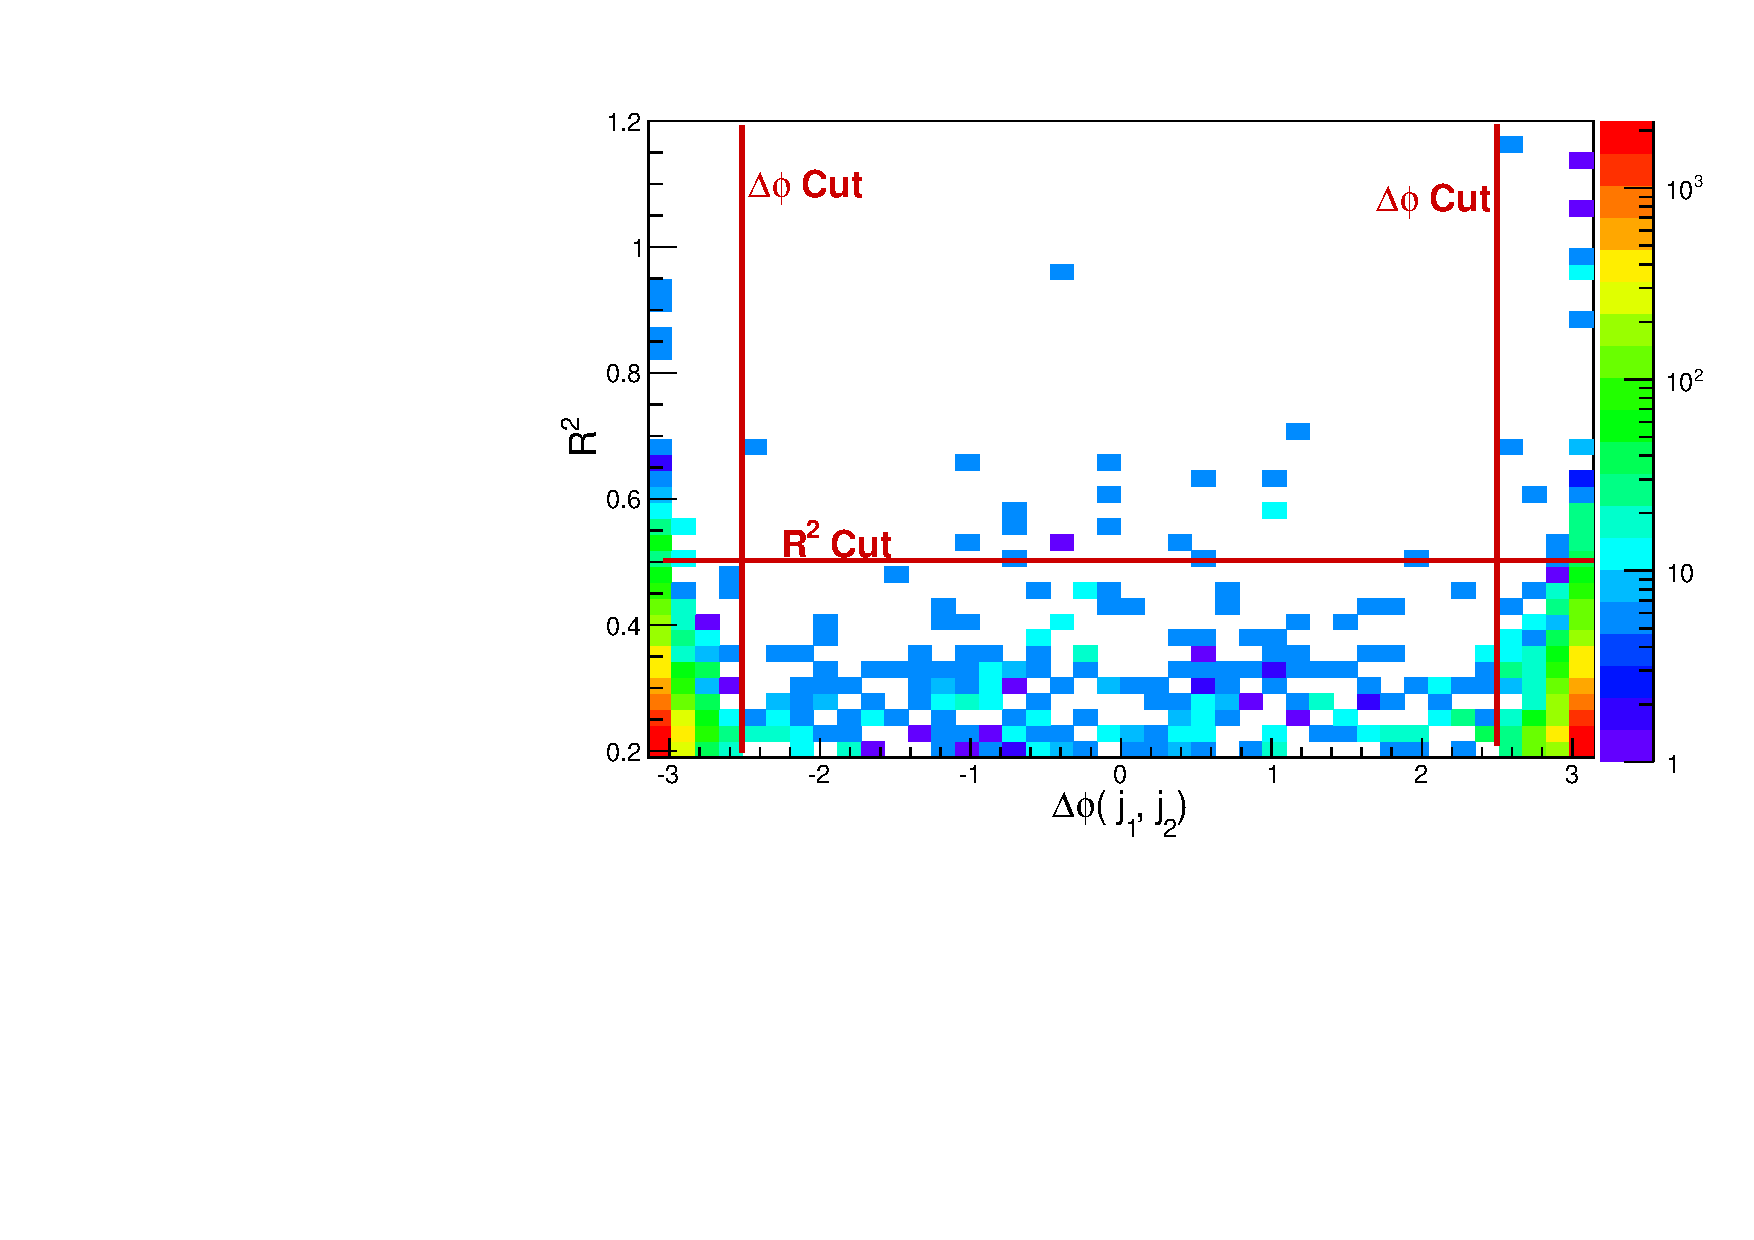
\includegraphics[trim = 2 0 0 0, clip = true,width=0.6\textwidth,angle=0.]{QCDplots/DPhi_R2_NoB_NoMu.pdf}\
\caption{ $\mathrm{R^2}$-$\Delta\phi  (J_{1}, J_{2})$ distribution for the QCD background in the $0\mu$ box.\label{dm:QCD2} }
\end{figure}
\begin{figure}[h]
\centering
\begin{tabular}{cc}
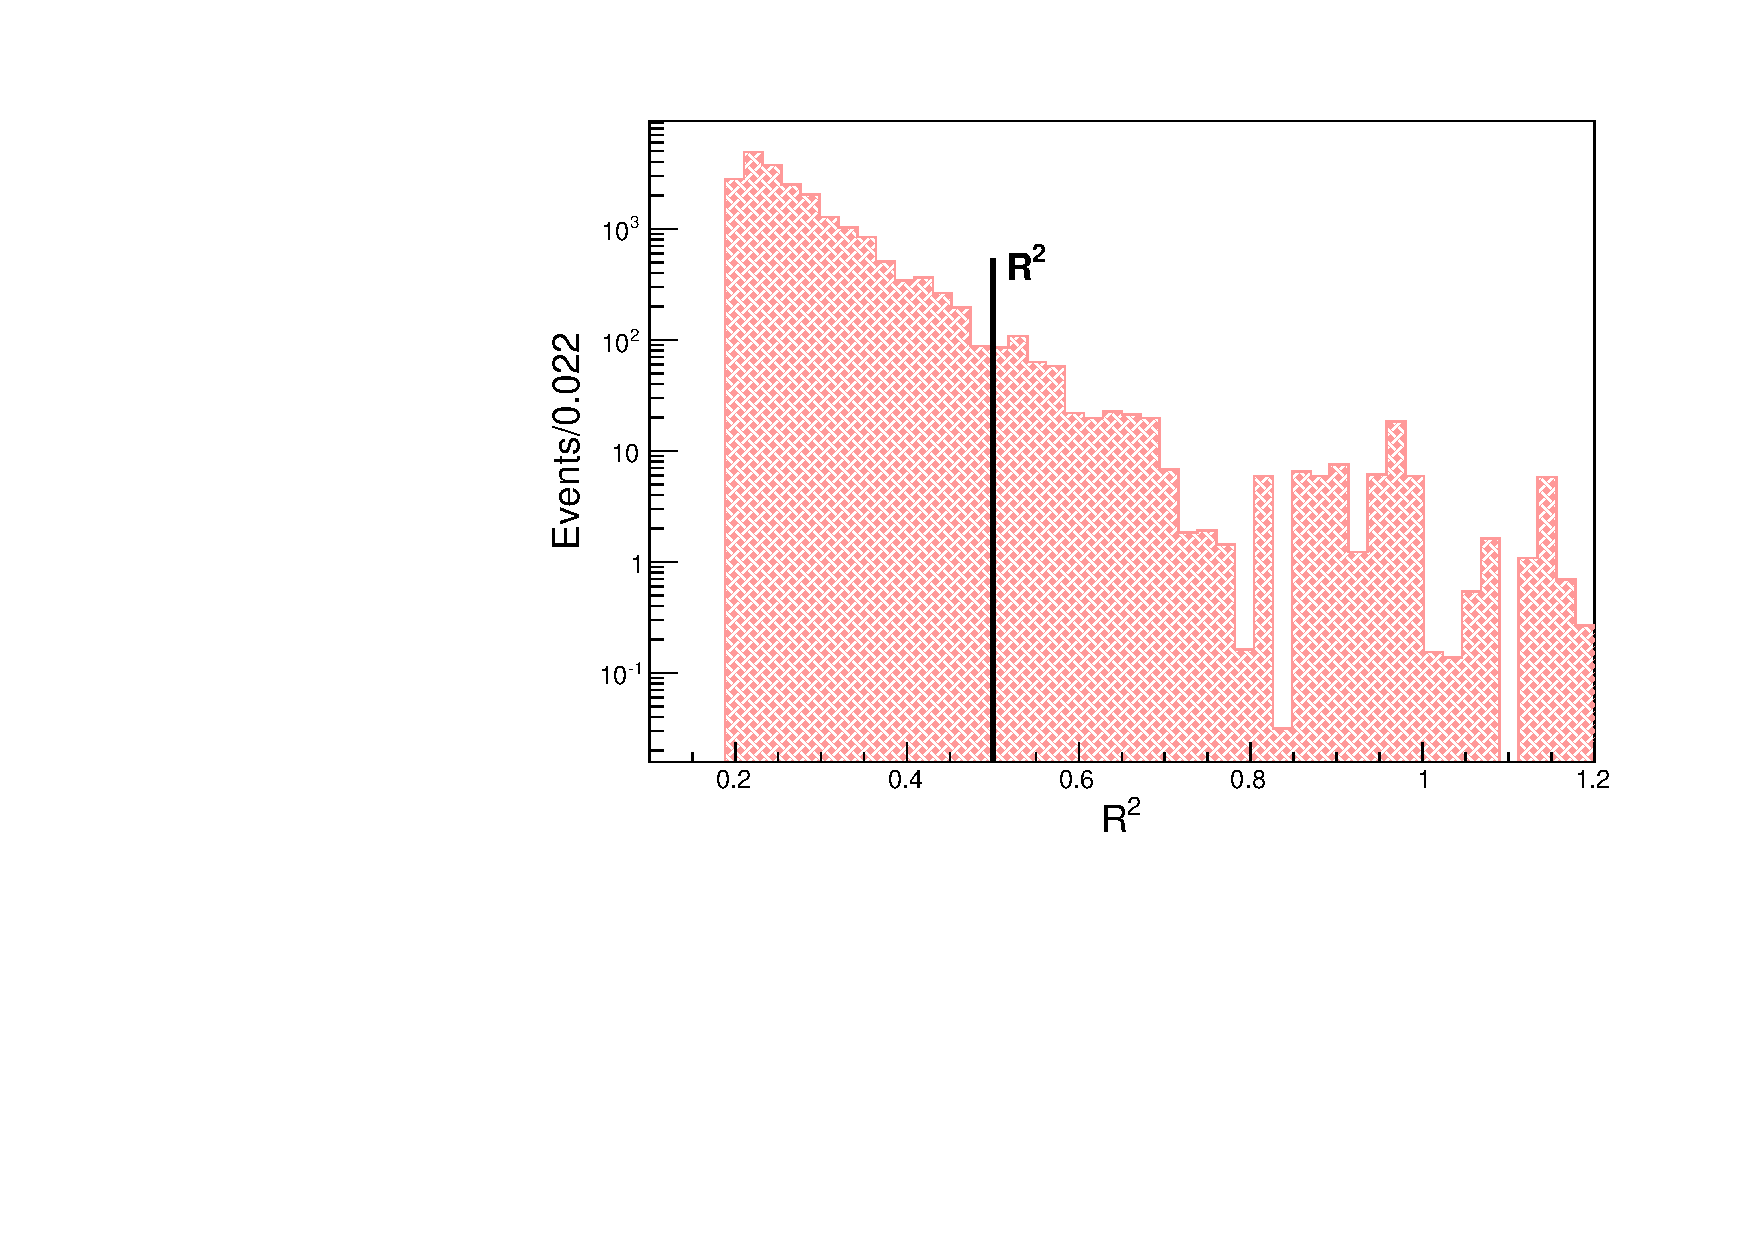
\includegraphics[trim = 2 0 0 0, clip = true, width=0.5\textwidth]{QCDplots/InclusiveR2_NoB_NoMu.pdf} &
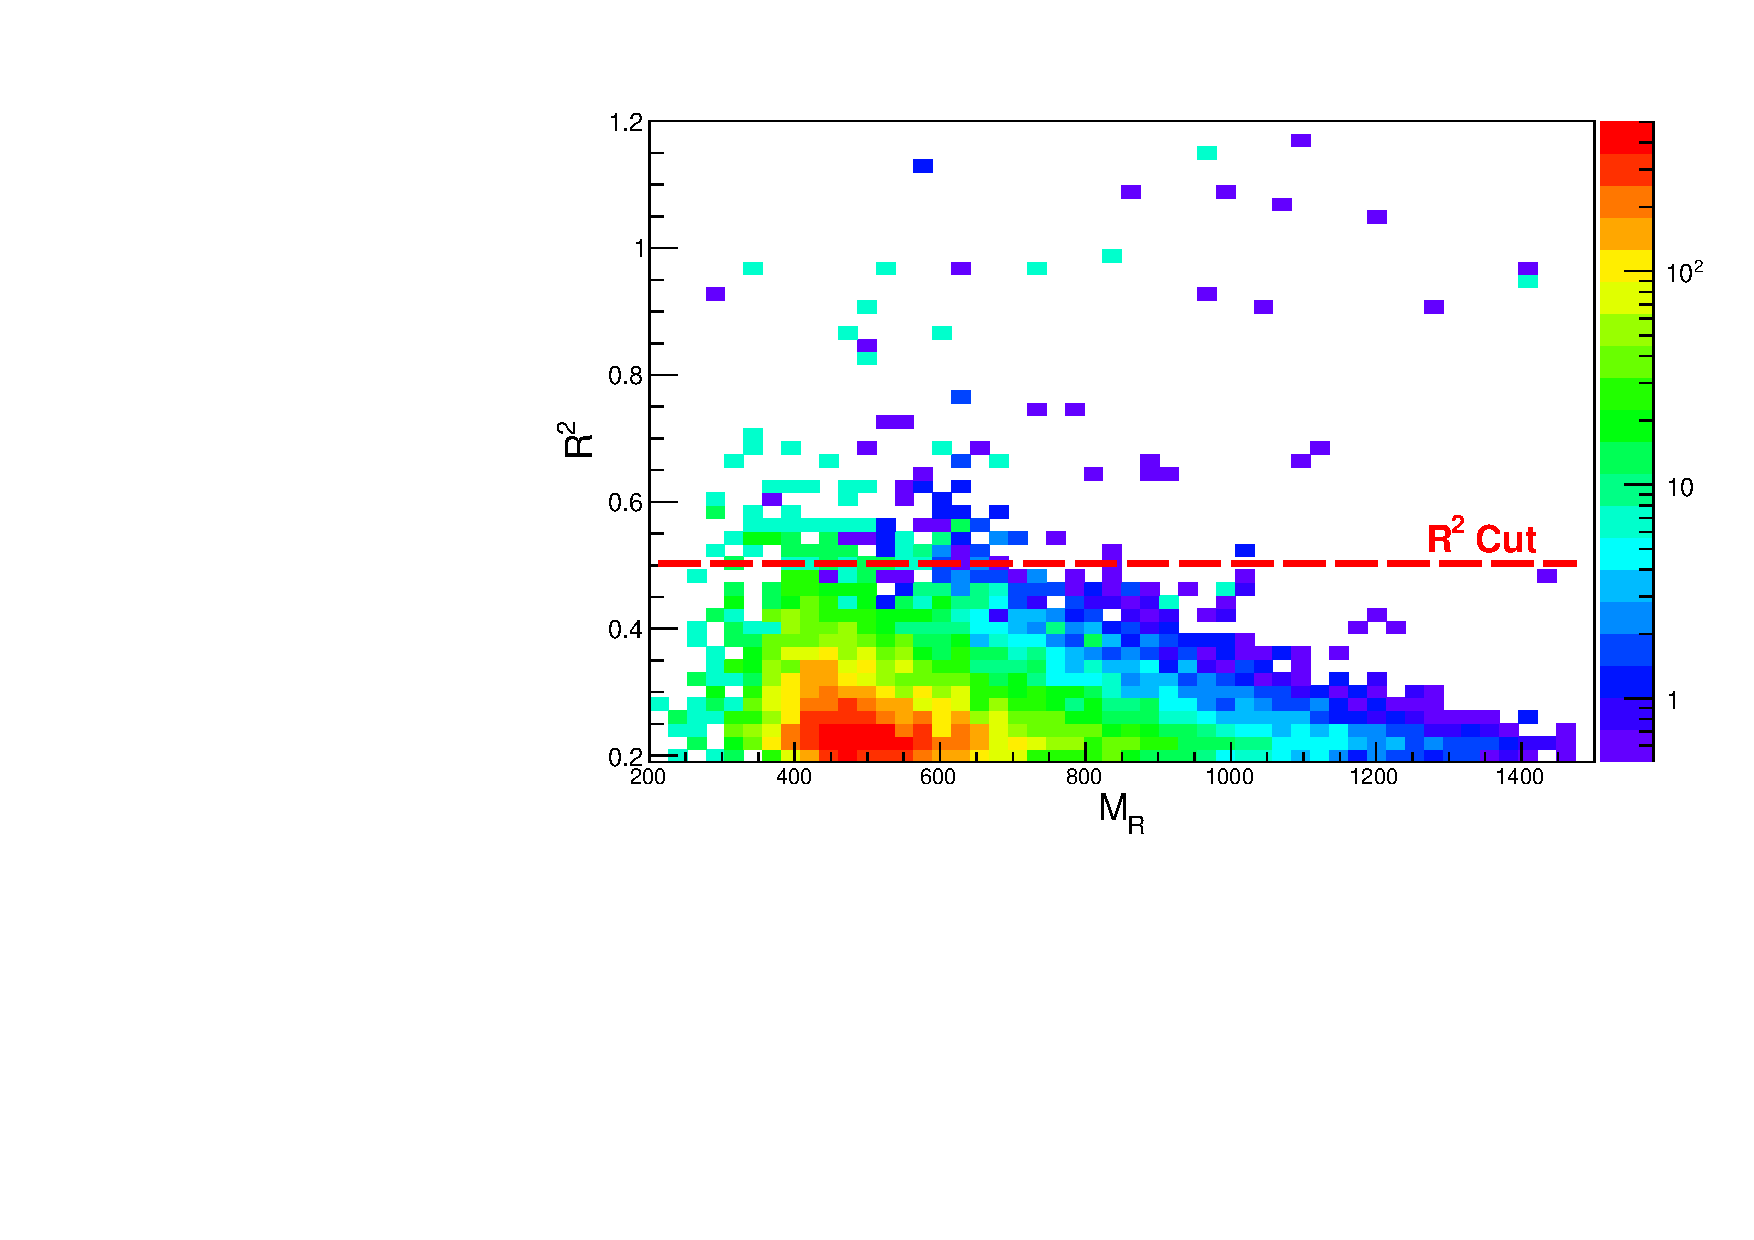
\includegraphics[trim = 2 0 0 0, clip = true, width=0.5\textwidth]{QCDplots/MR_R2_NoB_NoMu.pdf}\\
%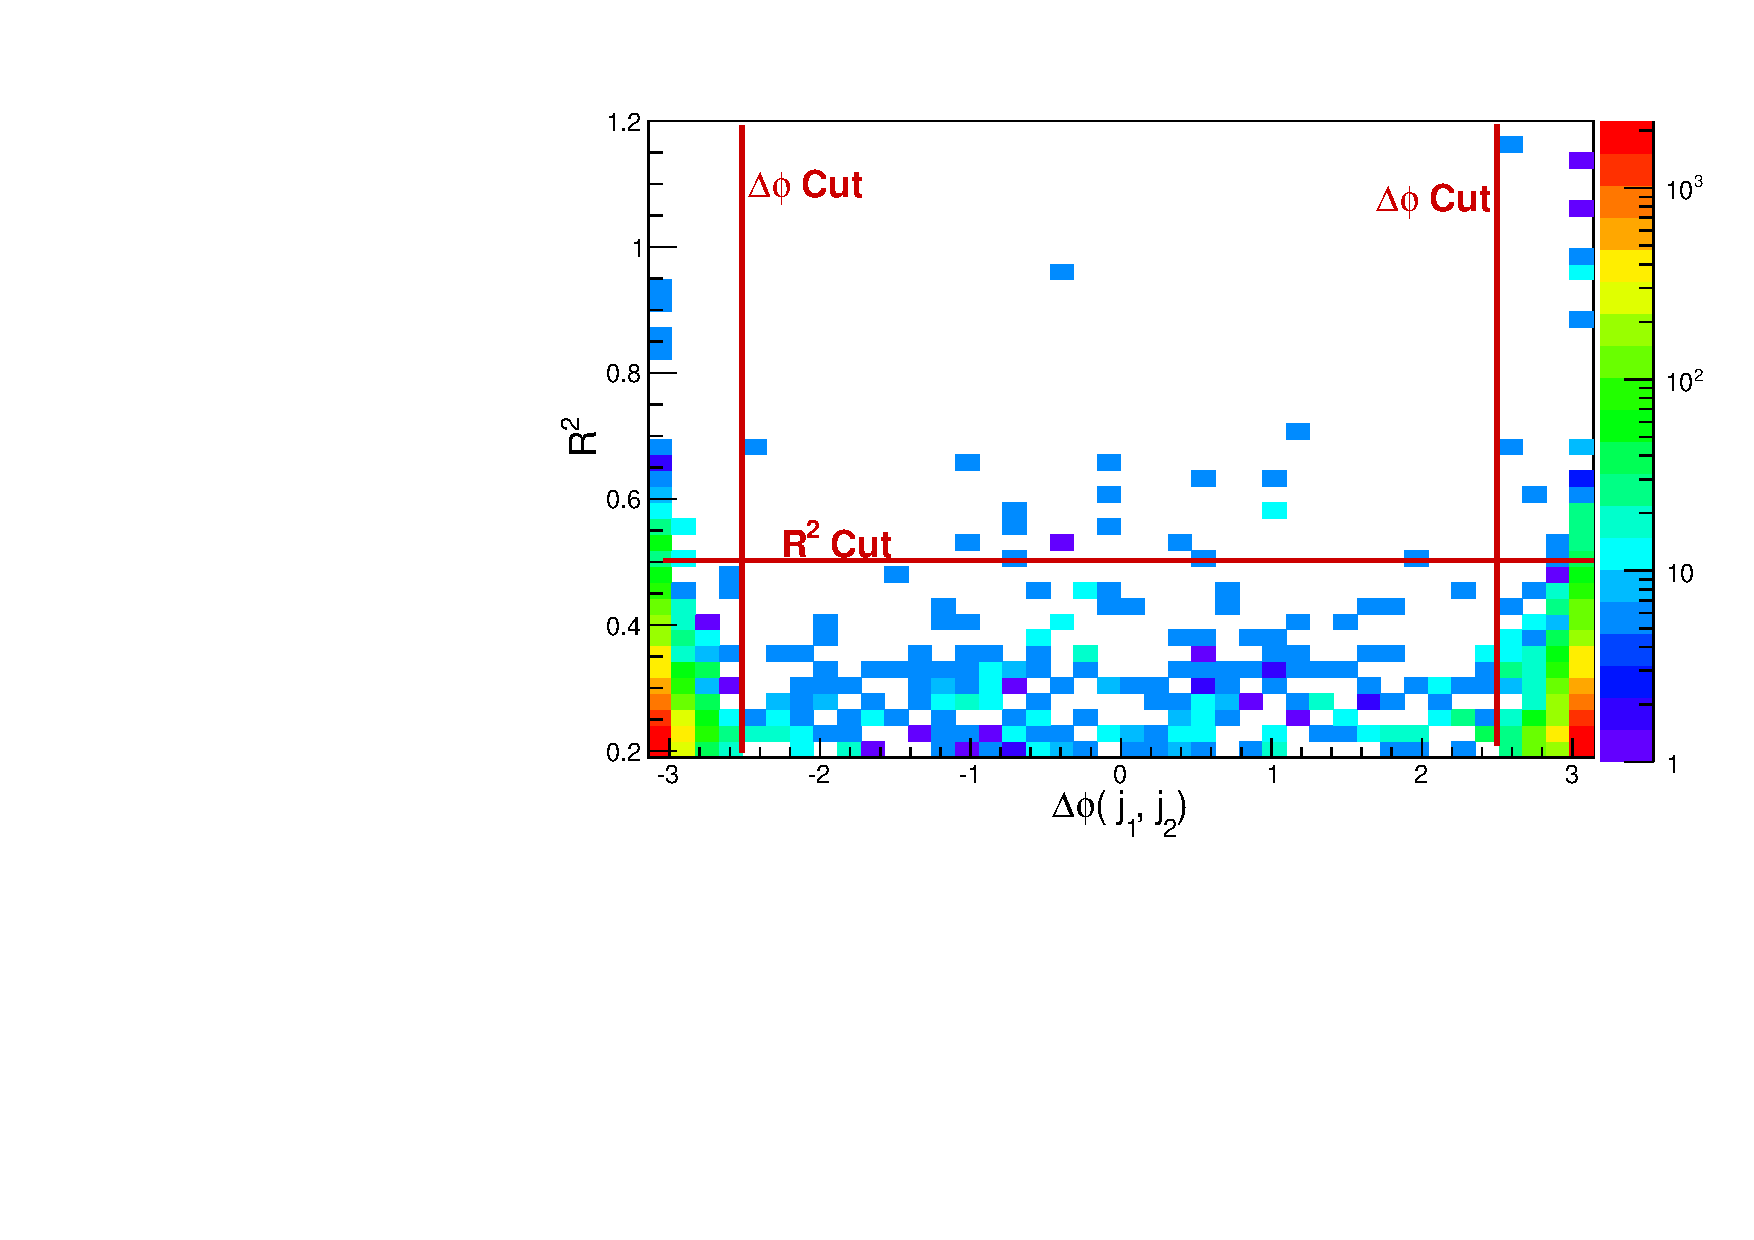
\includegraphics[trim = 2 0 0 0, clip = true,width=0.35\textwidth,angle=0.]{QCDplots/DPhi_R2_NoB_NoMu.pdf}\\
(a) & (b) \\
\end{tabular}
\caption{ (a) $\mathrm{R^2}$ and (b) $\mathrm{M_R}$-$\mathrm{R^2}$
  razor distributions for the QCD background in the $0\mu$ box.\label{dm:QCD1} }
\end{figure}

\subsection{Background estimation for the zero b-tag search region} 
\label{sec:bkgzmu}

To predict the background from $\PW(\ell\nu)$+jets and $\cPZ(\PGn\PAGn)$+jets in 
the zero b-tag search region, we use a data-driven method that extrapolates
the observed data yields in the 1$\mu$ control region to the search region.
Similarly, the observed yield in the 2$\mu$ control region allows the estimation of
the contribution from $\cPZ(\ell \ell)$+jets background process. Each
$\MR$ category is binned in $\RR^2$. 

The background expected from $\PW$ and $\cPZ$ boson production, in
each $\RR^2$ bin and in each $\MR$ category of the 0$\mu$
sample, is computed as
\begin{equation}
\footnotesize
  n_{i}^{0\mu} =  \Bigl(n_{i}^{1\mu} - N_{i}^{\ttbar,1\mu} - N_{i}^{\cPZ(\ell
    \ell)+\text{jets},1\mu}\Bigr) \frac{N_{i}^{\PW(\ell\nu)+\text{jets},0\mu}+N_{i}^{\cPZ(\PGn\PAGn)+\text{jets},0\mu}}{N_{i}^{\PW(\ell\nu)+\text{jets},1\mu}} +
\Bigl(n_{i}^{2\mu} - N_{i}^{\ttbar,2\mu}\Bigr) \frac{N_{i}^{\cPZ(\ell \ell)+\text{jets},0\mu}}{N_{i}^{\cPZ(\ell \ell)+\text{jets},2\mu}},
\label{eqn:pred}
\end{equation}
where $n_{i}^{k\mu}$ labels the data yield in bin $i$ for the sample
with $k$ muons, and $N_{i}^{X,k\mu}$ indicates the corresponding yield
for process $X$, derived from simulations. This background estimation method relies on 
the assumption that the kinematic properties of events in which $\PW$ and $\cPZ$ bosons are
produced are similar.

To estimate the accuracy of the background estimation method, we perform a cross-check 
by predicting the background in the 1$\mu$ control region using the observed data yield
in the 2$\mu$ control region. The Monte Carlo simulation is used to perform this extrapolation
analogous to the calculation in Equation~\ref{eqn:pred}.
The small contribution from the $\ttbar$ background process is also estimated using the simulated
samples. In Tables~\ref{tab:bkg1mu}~and~\ref{tab:bkg2mu}, the observed yields in the 1$\mu$ and 2$\mu$ control regions
respectively are compared to the estimate derived from data. In Tables~\ref{tab:bkg1mu}-\ref{tab:bkg0muWITHB}, 
the contribution of each process as predicted directly by simulated samples are also given.

\begin{table}[h]
  \topcaption{\label{tab:bkg1mu} Comparison of the observed yield in the
    1$\mu$ control region in each $\MR$ category and the
    corresponding data-driven background estimate obtained by extrapolating from the 2$\mu$ control region. The uncertainty in
    the estimates takes into account both the statistical
    and systematic components. The contribution of each individual background process is also shown, as
estimated from simulated samples, as well as the total MC predicted yield.}
\centering
\resizebox{\textwidth}{!}{
 \begin{tabular}{c*{6}{x}r}
   \hline
 \multicolumn{1}{c}{$\MR$ category} &  \multicolumn{1}{c}{$\cPZ(\PGn\PAGn)$+jets}  &  \multicolumn{1}{c}{$\PW(\ell
 \nu)$+jets}  &  \multicolumn{1}{c}{$\cPZ(\ell \ell)$+jets}  &  \multicolumn{1}{c}{$\ttbar$}  & \multicolumn{1}{c}{MC predicted}
 &\multicolumn{1}{c}{Estimated}  &  \multicolumn{1}{c}{Observed} \mT \mB\\
   \hline
   VL  &  0.7,0.3 & 4558,32 & 133,3 & 799,9 & 5491,33 & 5288,511 & 5926\mT\\
   L  &  0.5,0.3 & 1805,17 & 44,2 & 213,4 & 2063,18 & 1840,233 & 2110 \\
   H  &  0.1,0.1 & 915,11 & 16,1 & 66,2 & 997,11 & 629,240 & 923 \\
   VH  &   \multicolumn{1}{c}{$<$0.1}  & 183,5 & 2.6,0.2 & 8.5,0.8 & 194,5 & 166,93 & 143\mB\\
   \hline
 \end{tabular}
}
\end{table}

\begin{table}[h]
  \centering
  \topcaption{\label{tab:bkg2mu} Comparison of the observed yield for
    the 2$\mu$ control region in each $\MR$ category and the
    corresponding prediction from background simulation. The quoted uncertainty
    in the prediction reflects only the size of the simulated sample. The 
    contribution of each individual background process is also shown, as
    estimated from simulated samples.}
\resizebox{\textwidth}{!}{
 \begin{tabular}{*{6}{c}r}
   \hline
$\MR$  category&  $\cPZ(\PGn\PAGn)$+jets  &  $\PW(\ell
   \nu)$+jets  &  $\cPZ(\ell \ell)$+jets  &  $\ttbar$  &  MC predicted
   &  \multicolumn{1}{c}{Observed} \mT\mB\\
   \hline
   VL  &   $<$0.1  &  $<$0.1  & $214\pm4$ & $1.9\pm0.3$ & $215\pm4$ & 207\mT\\
   L  &    $<$0.1 & $0.4\pm0.3$ & $88\pm2$ & $0.5\pm0.2$ & $89\pm2$ & 78 \\
   H  &   $<$0.1  & $0.1\pm0.1$ & $48\pm1$ & $0.1\pm0.1$ & $48\pm1$ & 30 \\
   VH  &   $<$0.1  &  $<$0.1  & $10\pm1$ & $0.1\pm0.1$ & $10\pm1$ & 7\mB\\
   \hline
\end{tabular}
}
\end{table}

Figure~\ref{fig:1muCLOSURE} shows the comparison of the
$\RR^2$ distributions between the observed yield and the
data-driven background estimate in the 1$\mu$ control
region. The observed bin-by-bin difference is propagated as 
a systematic uncertainty in the data-driven background method,
and accounts for the statistical uncertainty in the 
event yield in the 2$\mu$ control region data as well as
potential differences in the modeling of the recoil spectra 
between $\PW$+jets and $\cPZ$+jets processes. Some bins exhibit 
relatively large uncertainties primarily due to statistical fluctuations
in the 2$\mu$ control region from which the background is prediction estimated. 
Though the uncertainties are rather large in fractional terms, 
sensitivity to DM signal models is still obtained, because of the enhanced 
signal to background ratio for the bins at large values of 
$\MR$ and $\RR^2$.



\begin{figure}
 \centering
   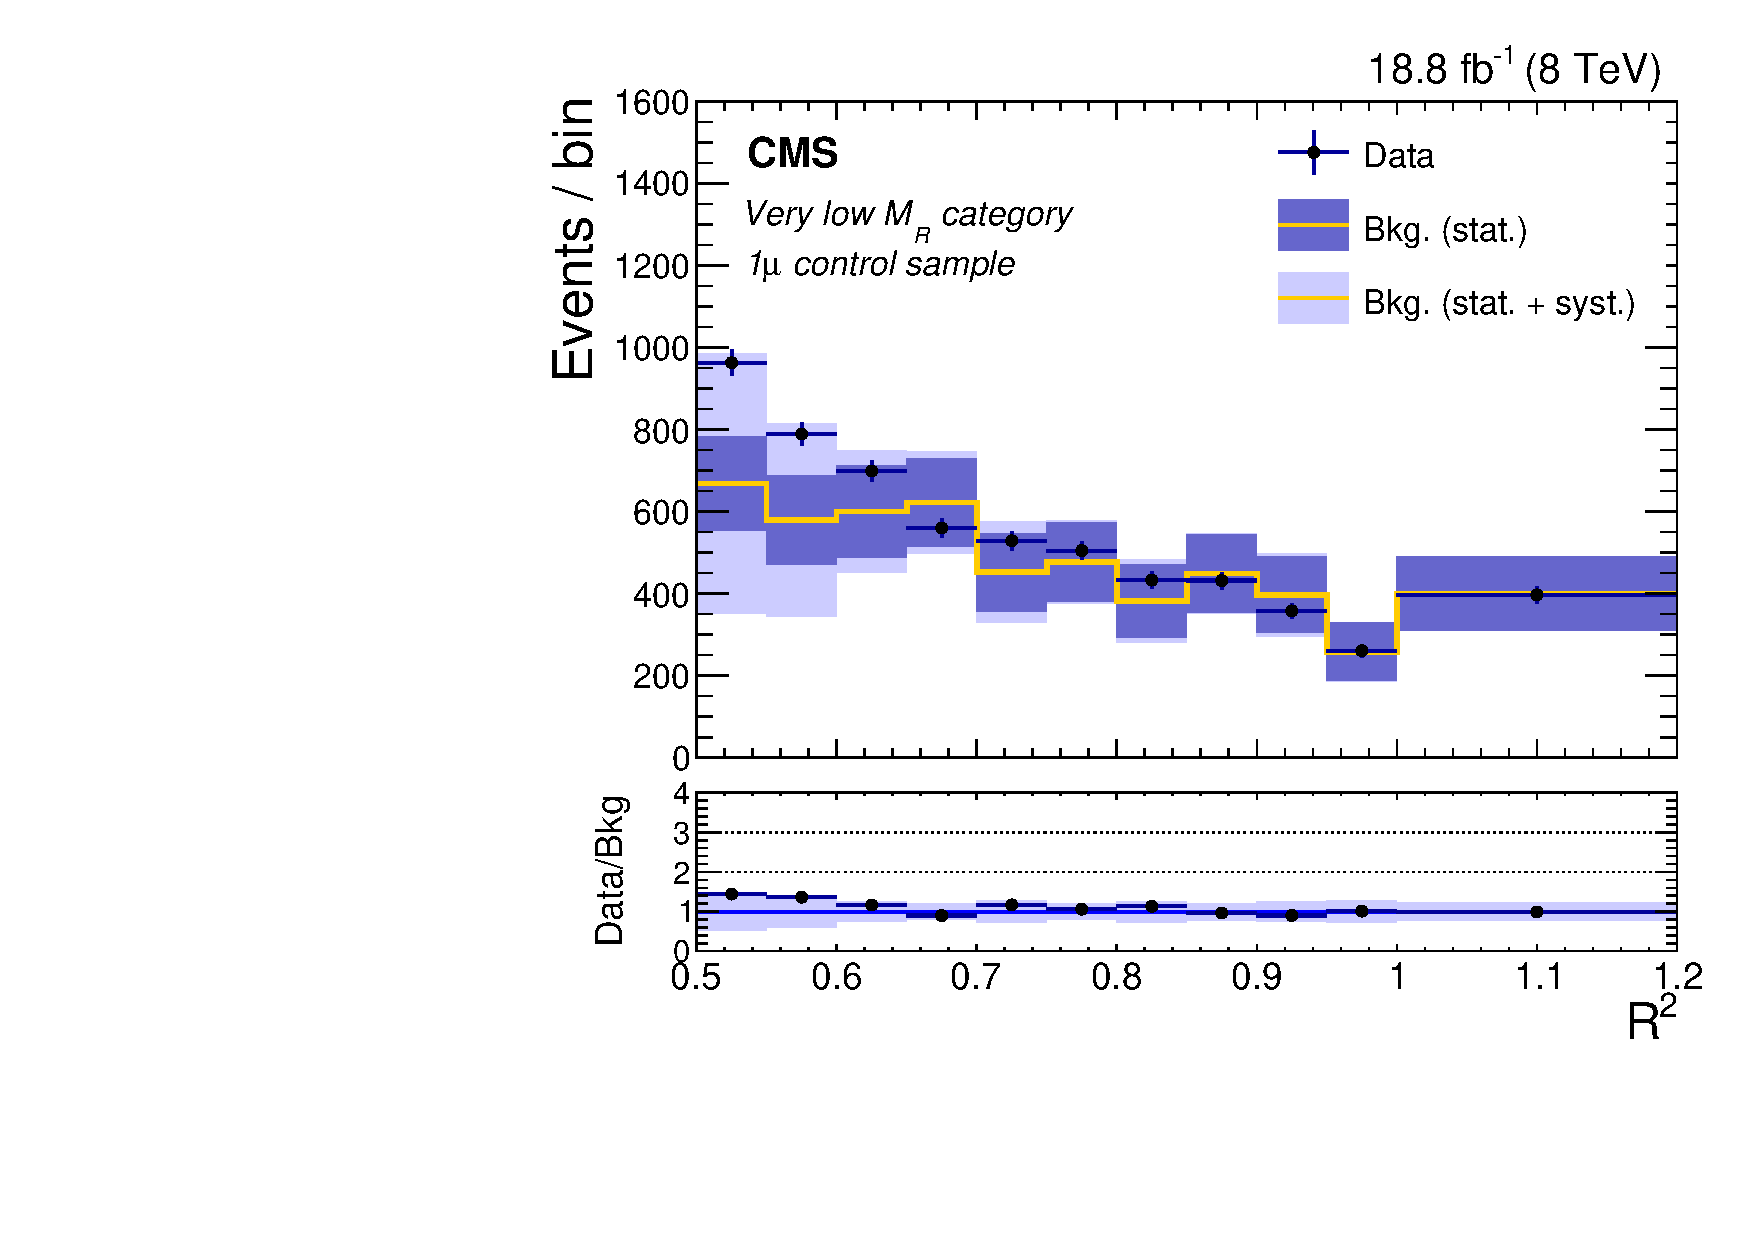
\includegraphics[width=0.48\textwidth]{PredPlotsAN_1MU_LE/OneMu_sys_cat_1.pdf}
   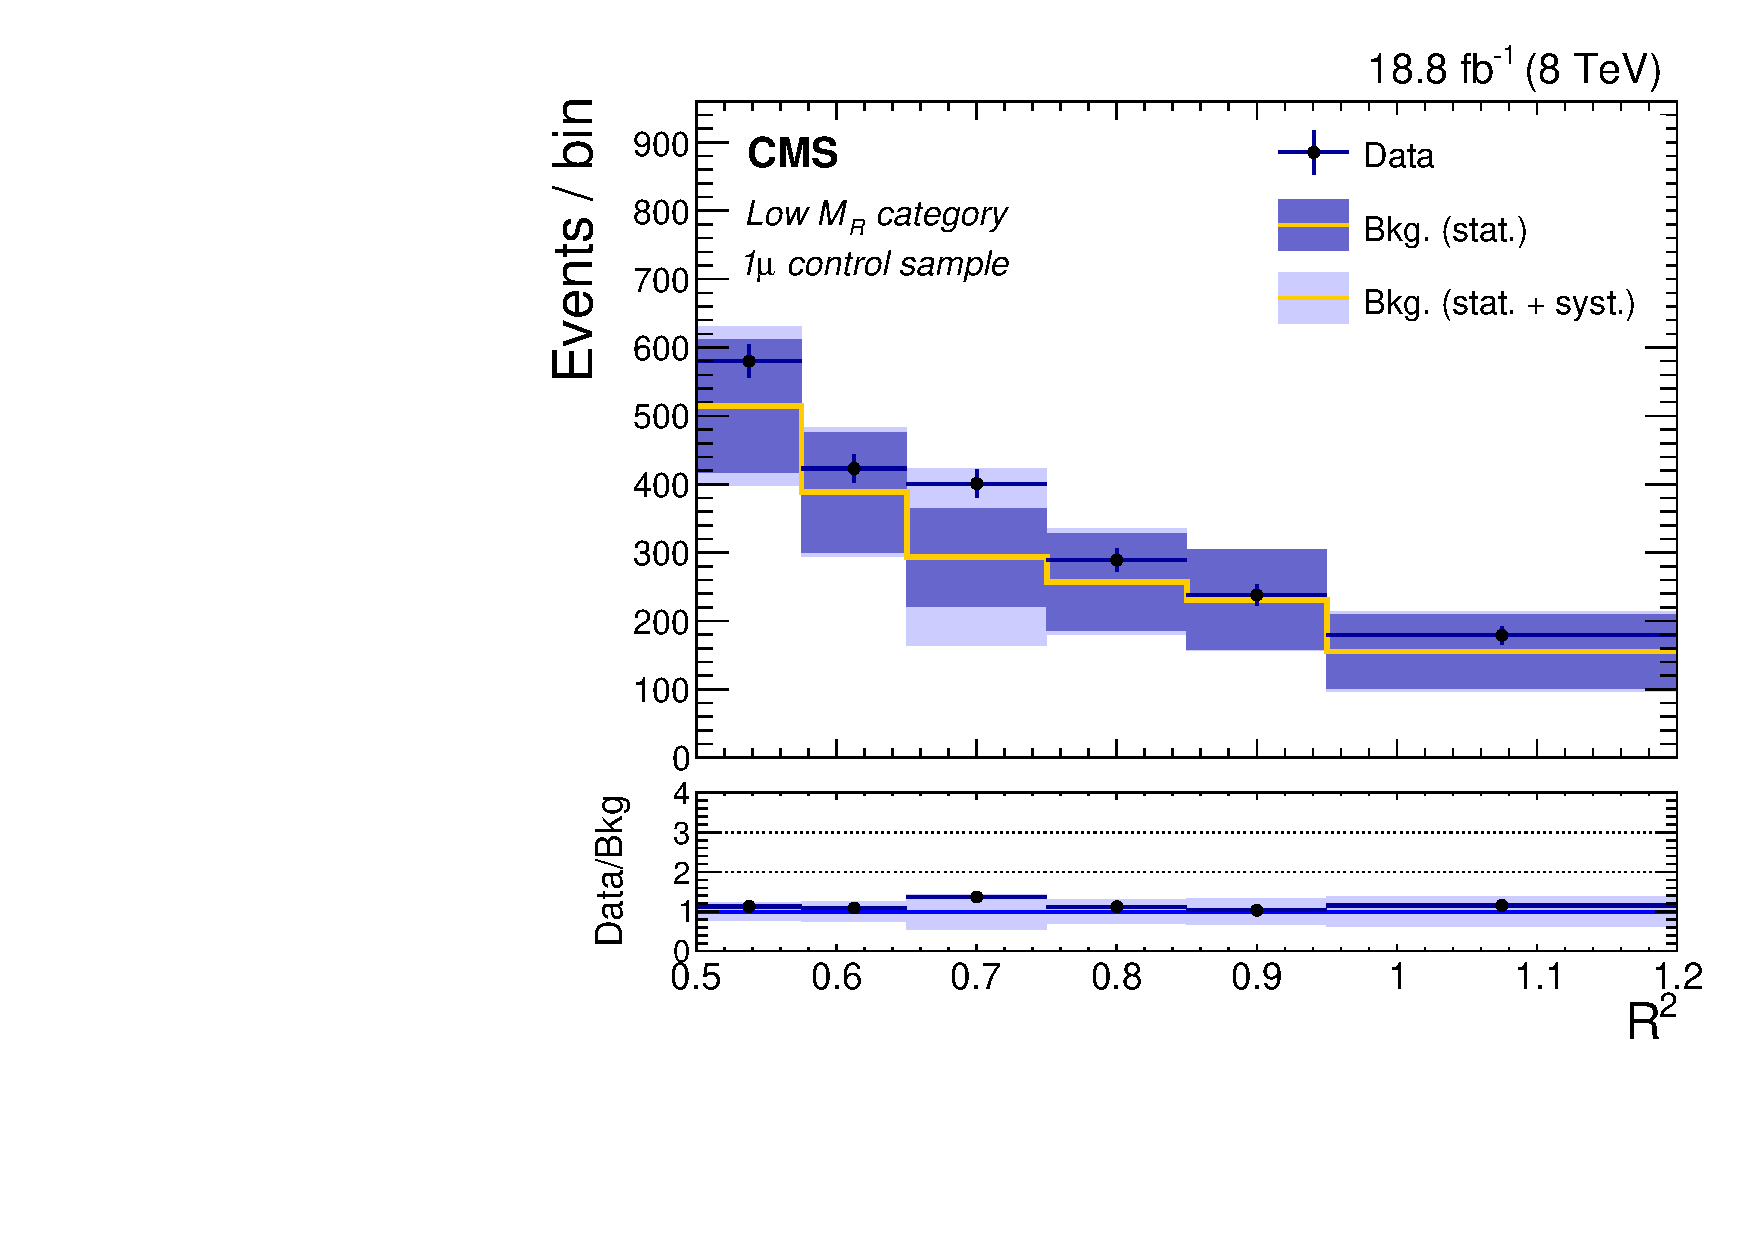
\includegraphics[width=0.48\textwidth]{PredPlotsAN_1MU_LE/OneMu_sys_cat_2.pdf}
   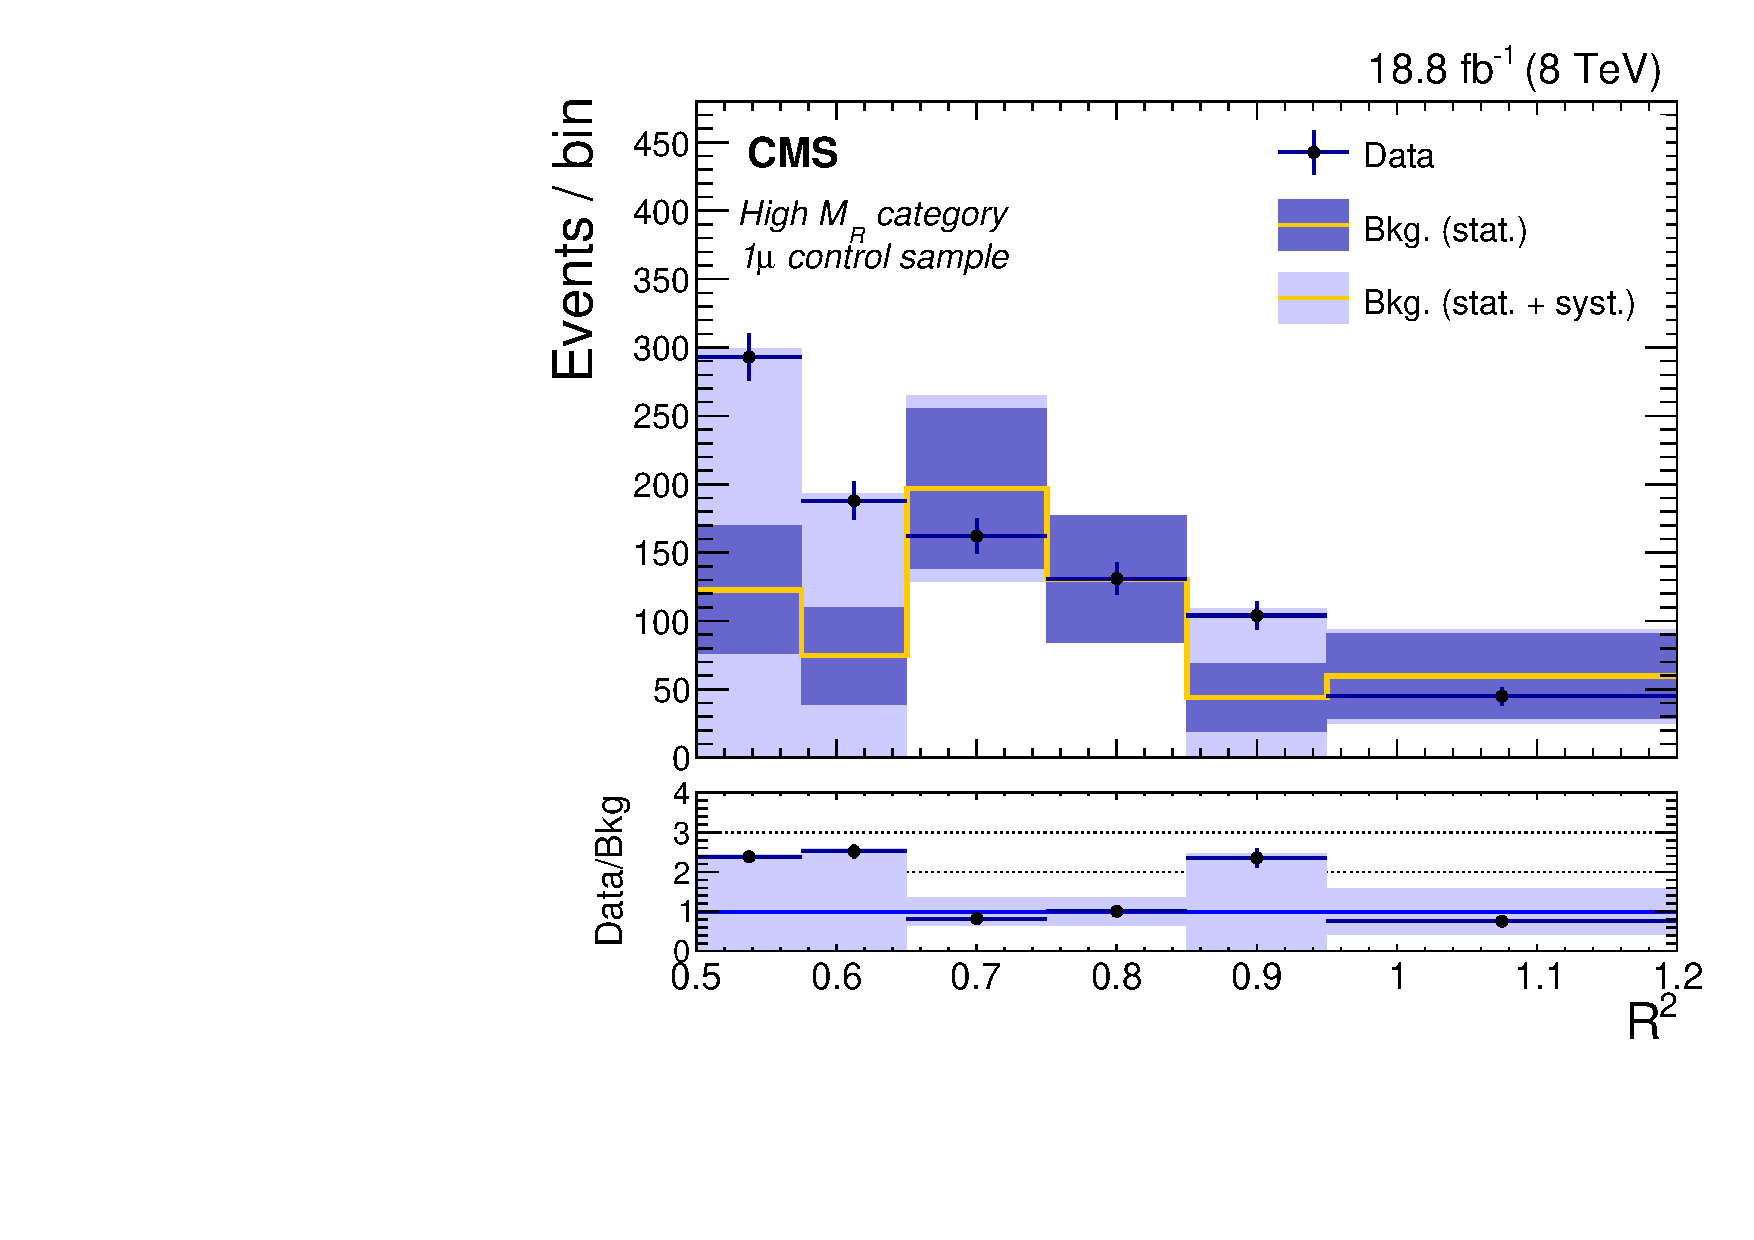
\includegraphics[width=0.48\textwidth]{PredPlotsAN_1MU_LE/OneMu_sys_cat_3.pdf}
   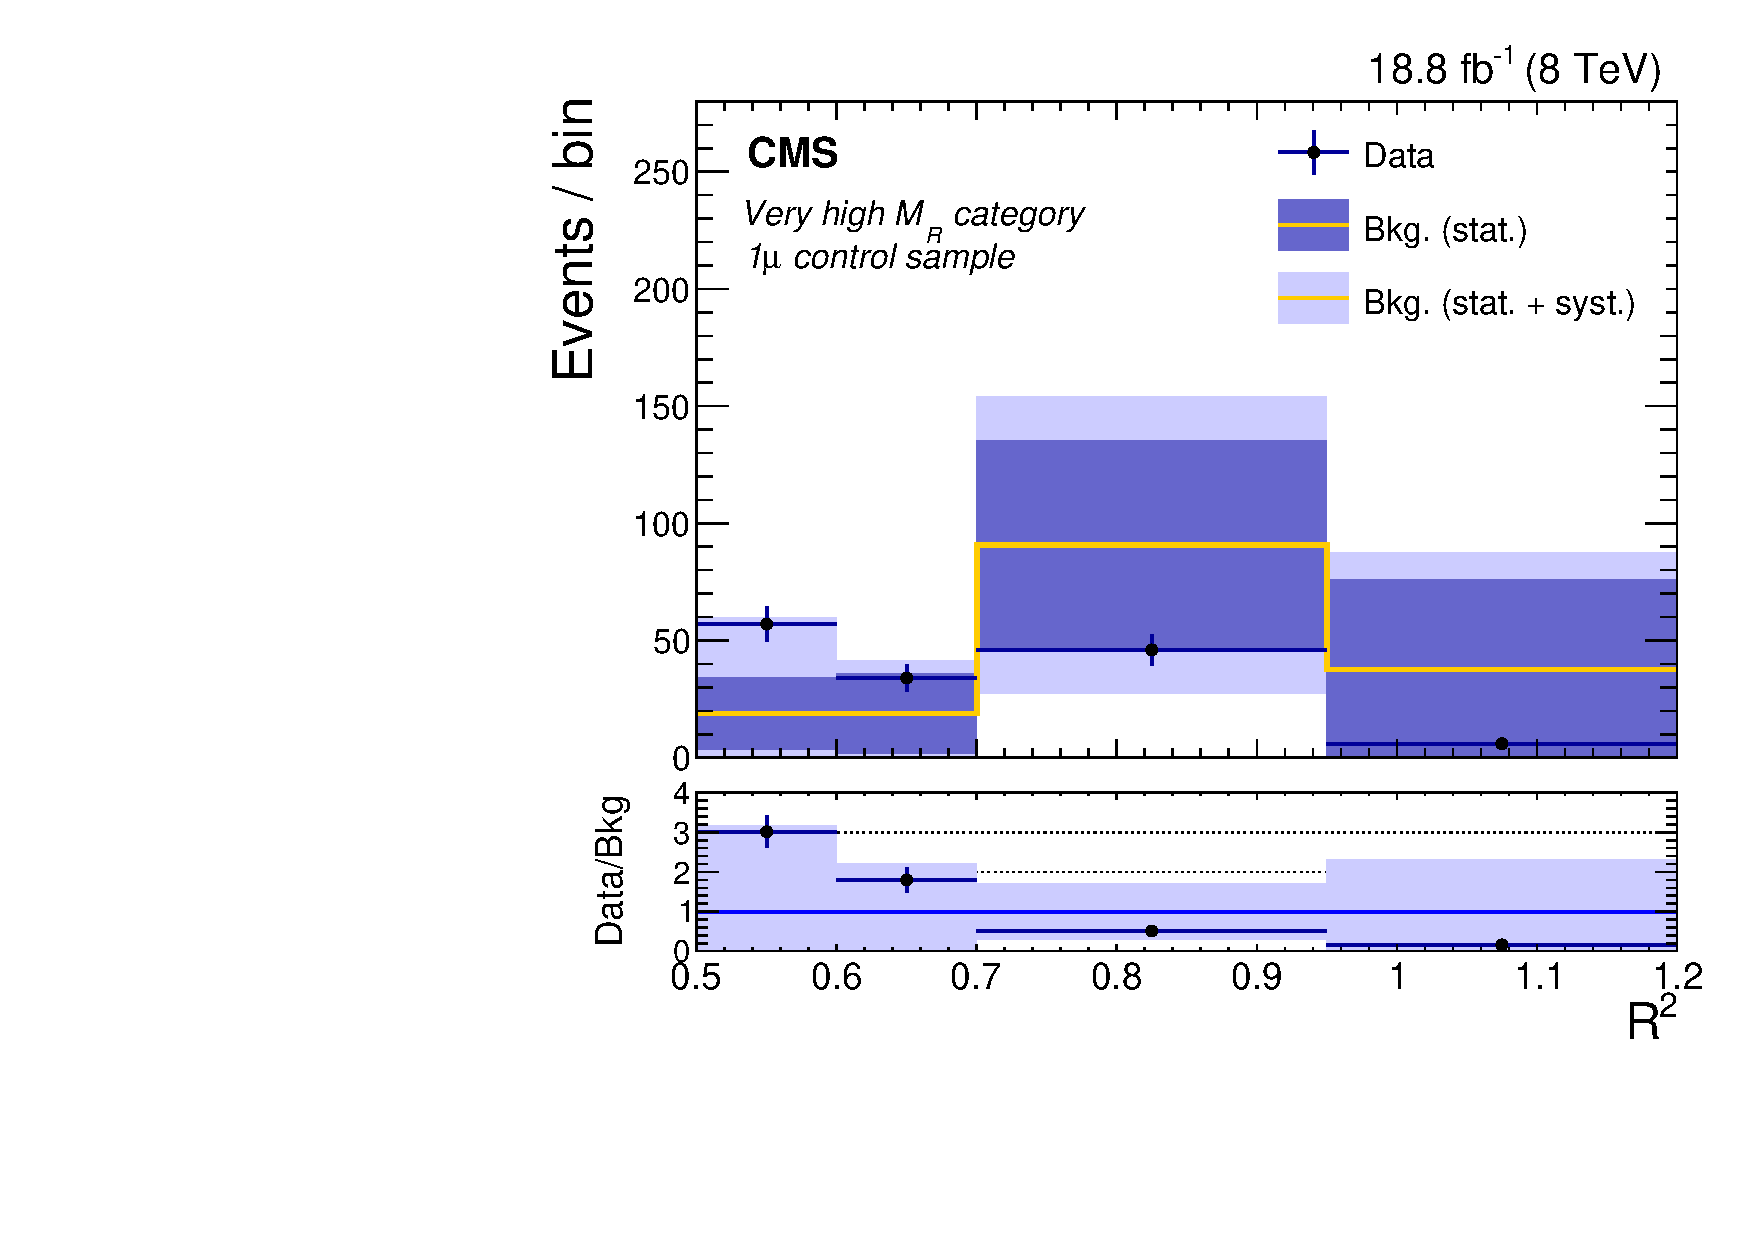
\includegraphics[width=0.48\textwidth]{PredPlotsAN_1MU_LE/OneMu_sys_cat_4.pdf}
 \caption{Comparison of observed yields in the 1$\mu$ control region and the
   data-driven background estimate derived from on the 2$\mu$ control region data in the four $\MR$ categories:
   VL (top left), L (top right), H (bottom left), and VH (bottom right). The bottom panel in each plot shows the
   ratio between the two distributions. The observed bin-by-bin
   deviation from unity is interpreted as an estimate of the systematic uncertainty
   associated to the background estimation methodology for the 0$\mu$ search region. The
   dark and light bands represent the statistical and the total
   uncertainties in the estimates, respectively. The horizontal bars indicate
the variable bin widths.\label{fig:1muCLOSURE}}
\end{figure}


The $\ttbar$ background is estimated using an analogous data-driven method,
where we derive corrections to the Monte Carlo simulation prediction
scaled to the $\ttbar$ production cross-section computed to NNLO accuracy~\cite{WatNNLO,ZatNNLO,TTbaratNNLO}
using data in the 2$\mu$b control region for each bin in $\RR^2$. 
The correction is then applied to the simulation prediction for
the $\ttbar$ background contribution to the zero b-tag search region.
This correction factor reflects potential mismodeling of the recoil
spectrum predicted by the Monte Carlo simulation. 
The contribution of each background process to
the 2$\mu$b sample, predicted from simulated samples, is given in
Table~\ref{tab:2mub}. The fraction of \ttbar events in the 2$\mu$b
control sample is ${\approx}95\%$. 
\begin{table}
\centering
\topcaption{\label{tab:2mub} Observed yield and predicted
    background from simulated samples in the 2$\mu$b control region.
    The quoted uncertainty in the prediction only reflects the size of the simulated sample. 
    The contribution of each individual background process is also shown,
    as estimated from simulated samples.}
\begin{tabular}{*{7}{c}}
  \hline
  Sample  &  $\cPZ(\PGn\PAGn)$+jets  &  $\PW(\ell \nu)$+jets &
  $\cPZ(\ell \ell)$+jets  &  $\ttbar$  & MC predicted &  Observed \mT\mB\\
  \hline
  2$\mu$b  &   $<$0.1  & $0.1\pm0.1$ & $2.2\pm0.3$ & $58\pm2$ & $60\pm2$ & 60 \mT\mB\\
  \hline
\end{tabular}
\end{table}
Figure~\ref{fig:2mub} shows the comparison of the observed
yield and the prediction from simulation, as a function of
$\RR^2$. We observe no significant deviations between the observed
data and the simulation prediction. The uncertainty derived from the 
data-to-simulation correction factor is propagated to the systematic uncertainty 
of the $\ttbar$ prediction in the zero b-tag search region. 

\begin{figure}
  \centering
   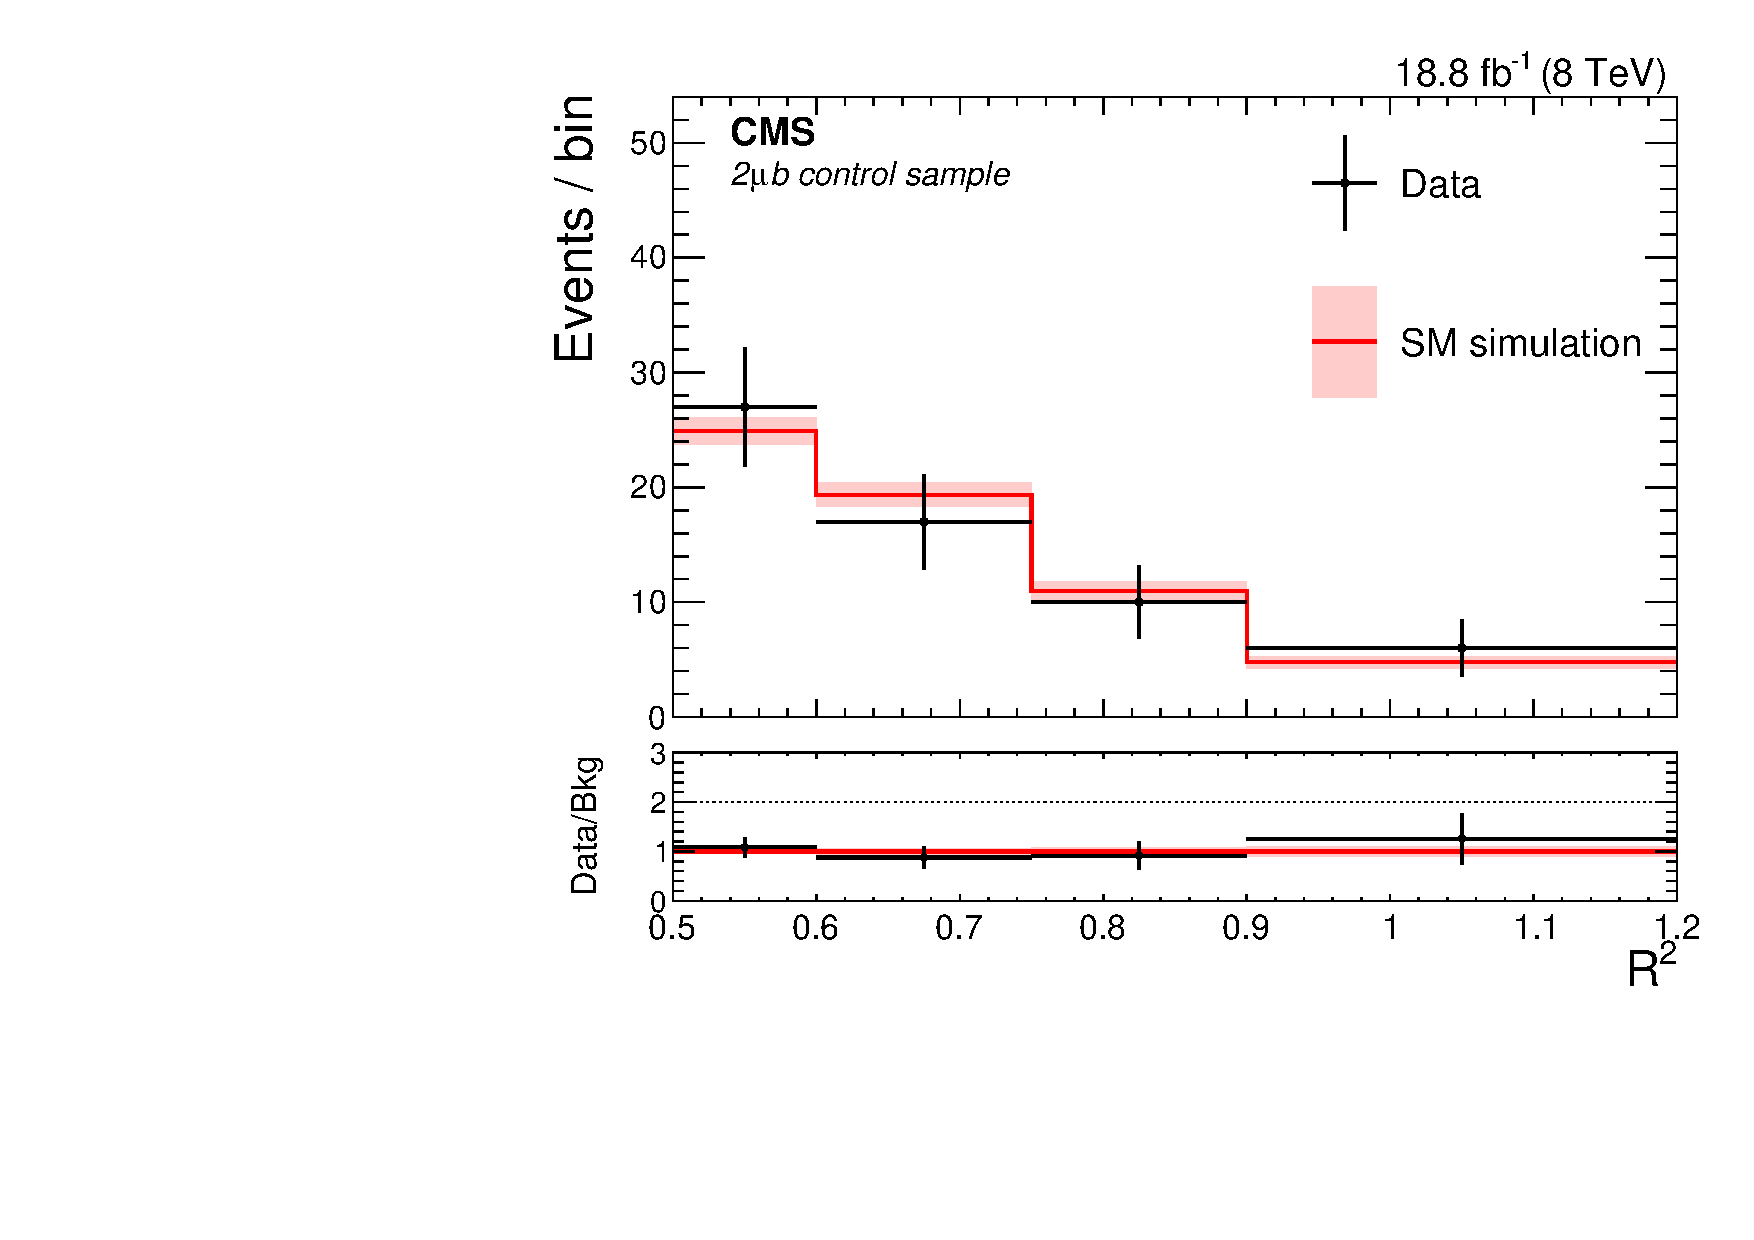
\includegraphics[width=0.47\textwidth]{BtagPlots/MC_CP_2Mu1TbTT_Sep.pdf}
   \caption{Comparison of the observed yield and the prediction from
     simulation as a function of $\RR^2$ in the 2$\mu$b control region.
     The uncertainties in the data and the simulated
     sample are represented by the vertical bars and the shaded bands,
     respectively. The horizontal bars indicate
the variable bin widths.\label{fig:2mub}}
\end{figure}
The result of the background estimation in the zero b-tag search region is given in
Table~\ref{tab:bkg0mu}, where it is compared to the observed yields in
data. The uncertainty in the background estimates takes into account
both the statistical and systematic components.
%The contribution of each process is also given,
%as predicted directly by simulated samples and therefore not used in
%the final result.
\begin{table}
\centering
\topcaption{\label{tab:bkg0mu}  Comparison of the observed yields for
  for the zero b-tag search region in each $\MR$ category and the
   corresponding background estimates. The uncertainty in
    the background estimate takes into account both the statistical
    and systematic components. The contribution of each individual background process is also shown, as
estimated from simulated samples, as well as the total MC predicted yield.}
\resizebox{\textwidth}{!}{
 \begin{tabular}{c*{6}{x}r}
  \hline
\multicolumn{1}{c}{$\MR$ category} &  \multicolumn{1}{c}{$\cPZ(\PGn\PAGn)$+jets}  &  \multicolumn{1}{c}{$\PW(\ell \nu)$+jets}  &  \multicolumn{1}{c}{$\cPZ(\ell \ell)$+jets}  &  \multicolumn{1}{c}{$\ttbar$}  & \multicolumn{1}{c}{MC predicted}&  \multicolumn{1}{c}{Estimated}  &  \multicolumn{1}{c}{Observed} \mT\mB\\
  \hline
  VL  &  6231,37  & 4820,33 & 49,2 & 555,7 & 11655,50 &12770,900 & 11623 \mT\\
  L  &  2416,19 & 1513,16 & 11,1 & 104,3 & 4044,25 & 4170,270 & 3785 \\
  H  &  1127,7 & 625,9 & 2.9,0.3 & 24,1  &  1779,12 & 1650,690 & 1559 \\
  VH  &  229,2 & 103,3 & 0.2,0.1 & 3.1,0.5 &
   335,3 & 240,160 & 261\mB\\
  \hline
\end{tabular}
}
\end{table}
The comparison of the data-driven background estimates and the observations for
each $\MR$ category is shown in Fig.~\ref{fig:0muSignalBkg1GeV}, as a function of $\RR^2$. 
The expected event distribution is shown for two signal
benchmark models, corresponding to the pair production of DM particles
of mass 1\GeV in the effective field theory (EFT) approach with vector coupling to u or d quarks. 
Details on the signal benchmark models are given in Section~\ref{sec:EFT0mu}.
\begin{figure}
 \centering
   \includegraphics[width=0.48\textwidth]{SignalBkgPlots/Data_MC_cat1_1_DoubleSignal_V.pdf}
   \includegraphics[width=0.48\textwidth]{SignalBkgPlots/Data_MC_cat2_1_DoubleSignal_V.pdf}
   \includegraphics[width=0.48\textwidth]{SignalBkgPlots/Data_MC_cat3_1_DoubleSignal_V.pdf}
   \includegraphics[width=0.48\textwidth]{SignalBkgPlots/Data_MC_cat4_1_DoubleSignal_V.pdf}
 \caption{Comparison of the observed yield in the zero b-tag control region and the
   background estimates in the four $\MR$ categories:
   VL (top left), L (top right), H (bottom left), and VH (bottom right). The
   contribution of individual background processes is shown by the
   filled histograms. The bottom panels show the ratio
   between the observed yields and the total background estimate. For reference, the distributions from two
   benchmark signal models are also shown, corresponding to the pair
   production of DM particles of mass 1\GeV in the EFT approach with
   vector coupling to u or d quarks. The horizontal bars indicate
the variable bin widths.\label{fig:0muSignalBkg1GeV} }
\end{figure}


\subsection{Background estimation for the \texorpdfstring{0$\mu$b and 0$\mu$bb}{0 mu b and 0 mu bb} samples}

A similar data-driven technique is used to determine the expected background for the 
one and two b-tag search regions. The background from $\ttbar$ events for each $\RR^2$ bin in the
one b-tag search region, $n(\ttbar)_{i}^{0\mu\PQb}$, is computed as:
\begin{equation}
  n(\ttbar)_{i}^{0\mu\PQb} =  \bigl(n(\ttbar)_{i}^{2\mu\PQb} - N_{i}^{\cPZ(\ell
    \ell)+\text{jets},2\mu\PQb} - N_{i}^{\PW(\ell\nu)+\text{jets},2\mu\PQb}\bigr)
\frac{N(\ttbar)_{i}^{0\mu\PQb}}{N(\ttbar)_{i}^{2\mu\PQb}}\label{eq:bBkgPred}
\end{equation}
where $n(\ttbar)_{i}^{2\mu\PQb}$ is the observed yield in the $i$th $\RR^2$
bin in the 2$\mu$b control region, while $N(\ttbar)_{i}^{0\mu\PQb}$ and
$N(\ttbar)_{i}^{2\mu\PQb}$ are the $\ttbar$ yields in the $i$th $\RR^2$ bin 
predicted by the simulation for the one b-tag search region and the 2$\mu$b control region
respectively. Similarly, the \ttbar background in the two b-tag search region
is derived from Eq.~(\ref{eq:bBkgPred}), replacing $N(\ttbar)_{i}^{0\mu\PQb}$ 
with $N(\ttbar)_{i}^{0\mu\mathrm{bb}}$, the \ttbar
background yield in the $i$th bin of the two b-tag search region predicted
by the simulation. The data yield in the 2$\mu$b control region is
corrected to account for the small contamination from $\cPZ$+jets and
$\PW$+jets, predicted with the simulated yields $N_{i}^{\cPZ(\ell\ell)+\text{jets},2\mu\PQb}$ and
$N_{i}^{\PW(\ell\nu)+\text{jets},2\mu\PQb}$, respectively.


The background contribution from $\PW(\ell \nu)$+jets and $\cPZ(\PGn\PAGn)$+jets events is 
predicted using the $\cPZ(\mu\mu)$b control region, and summarized in Table~\ref{tab:WITHB}.
The $\cPZ$+jets purity of this control region is ${\approx}$89\%. 
The observed yield in the $\cPZ(\mu\mu)$b control region is shown in the left plot of Fig.~\ref{fig:Zmumub}, 
as a function of $\RR^2$, along with the Monte Carlo simulation prediction. The uncertainty on the
simulation prediction accounts only for the statistical uncertainty of the simulated sample.
This contribution, scaled by the ratio of the predicted V+jets background in the search regions 
to that in the control region, obtained from simulation, provides an estimate for each $\RR^2$ bin. 

\begin{table}
\centering
\topcaption{\label{tab:WITHB}
    Comparison of the observed yields in the $\cPZ(\mu\mu)$b and
    $1\mu$b samples, the corresponding predictions from background
    simulation, and (for $1\mu$b only) the cross-check background
    estimate. The contribution of each individual background process is also shown, as
estimated from simulated samples.}
\resizebox{\textwidth}{!}{
\begin{tabular}{*{7}{c}r}
  \hline
  Sample  &  $\cPZ(\PGn\PAGn)$+jets  &  $\PW(\ell \nu)$+jets  &
  $\cPZ(\ell \ell)$+jets  &  $\ttbar$   &  MC predicted  & Estimated &
  \multicolumn{1}{c}{Observed} \mT\mB\\
  \hline
   $\cPZ(\mu\mu)$b  &  $<$0.1  &  $<$0.1  & $134\pm3$ & $17\pm1$ &
   $151\pm3$ &\NA  &  175 \mT\mB\\
   $1\mu$b &  $0.2\pm0.1$ & $279\pm7$ & $11\pm1$ & 3038 $\pm$
   17 & $3328\pm18$ & $3410\pm540$ & 2920\mT\mB\\
  \hline
\end{tabular}
}
\end{table}
\begin{figure}
\centering
   \includegraphics[width=0.48\textwidth]{BtagPlots/MC_CP_2Mu1LbZ_Sep.pdf}
   \includegraphics[width=0.48\textwidth]{BtagPlots/Closure_CP_1mu1Tb_SYS_Sep.pdf}
 \caption{Comparison of the observed yield and the
   prediction from simulation in the $\cPZ(\mu\mu)$b control sample (left)
   and of the observed yield in the $1\mu$b control sample and
   the background estimates from the 2$\mu$b and $\cPZ(\mu\mu)$b
   control samples (right), shown as a function of $\RR^2$. The bottom
   panel of each figure shows the ratio between the data and the
   estimates. The shaded bands represent the statistical uncertainty
   in the left plot, and the total uncertainty in the right plot. The horizontal bars indicate
the variable bin widths.\label{fig:Zmumub}}
\end{figure}

We perform a cross-check of the method on the 1$\mu$b control region
by predicting the background from the 2$\mu$b control region data.
The data and prediction are compared on the right of Fig.~\ref{fig:Zmumub},
where we observe reasonable agreement. The difference between the 
prediction and the observed data in this cross-check region is propagated as a
systematic uncertainty of the method. 

The estimated background in the one and two b-tag search regions
is given in Table~\ref{tab:bkg0muWITHB} and shown in Fig.~\ref{fig:0muttbar}, where it is compared to
the observed yields in data. The uncertainty in the
estimates take into account both the statistical and systematic
components.% In the table, the yield expected from simulation is
\begin{figure}
   \includegraphics[width=0.48\textwidth]{BtagPlots/Bkg_0mu2TbEXC_CP.pdf}
   \includegraphics[width=0.48\textwidth]{BtagPlots/Bkg_0mu1TbEXC_CP.pdf}
 \caption{Comparison of observed event yields and background
   estimates as a function of $\RR^2$, for the
   one (left) and two (right) b-tag search regions.
   The shaded bands represent the total uncertainty in the estimate. The horizontal bars indicate
the variable bin widths.\label{fig:0muttbar}}
\end{figure}
\begin{table}
\centering
  \topcaption{ Comparison of the observed yield for
    events in the one and two b-tag search regions and the corresponding background
    estimates. The uncertainty in the estimates takes into account
    both the statistical and systematic components. The contribution of each individual background process is also shown, as
estimated from simulated samples, as well as the total MC predicted yield.
\label{tab:bkg0muWITHB}}
\resizebox{\textwidth}{!}{
\begin{tabular}{*{7}{c}r}
  \hline
 Sample  &  $\cPZ(\PGn\PAGn)$+jets  &  $\PW(\ell \nu)$+jets  &
  $\cPZ(\ell \ell)$+jets  &  $\ttbar$  & MC predicted& Estimated &  \multicolumn{1}{c}{Observed} \mT\mB\\
\hline
  $0\mu$bb  &  $44\pm3$  &  $14\pm2$  &  $0.2\pm0.1$  &  204
  $\pm$ 4  & $262\pm5$ &  $271\pm37$  &  247 \mT\mB\\
  $0\mu$b  &  $417\pm8$  &  $216\pm7$  &  $2.4\pm0.4$  &  $1480\pm12$  & $2115\pm16$ &  $2230\pm280$  &  2282 \mT\mB\\
\hline
\end{tabular}
}
\end{table}




\section{Systematic uncertainties}\label{sec:sys}

For each $\RR^2$ bin in each $\MR$ category, the
difference between the observed and estimated yields in the
crosscheck analysis (see Section~\ref{sec:bkg}) is taken as the estimate of the uncertainty associated with the
method. The uncertainty is found to
be typically ${\approx}$20--40\%, depending on the considered bin in the
($\MR$, $\RR^2$) plane. Other sources of systematic uncertainties such
as the modeling of the jet energy scale correction, and the initial-state
radiation in the event are found to be negligible compared to the
systematic from the
cross-check. Figures~\ref{dm:ccJES} and ~\ref{dm:ccISR} show the indiviual systematic uncertaintes just
mentioned and the systematic uncertainty from the cross-check.

\begin{figure}[ht!]
 \centering
 \begin{tabular}{cccc}
   \includegraphics[width=0.4\textwidth]{SysPlots/cat1_JES.pdf}&
   \includegraphics[width=0.4\textwidth]{SysPlots/cat2_JES.pdf}\\
   (a) & (b)\\
   \includegraphics[width=0.4\textwidth]{SysPlots/cat3_JES.pdf}&
   \includegraphics[width=0.4\textwidth]{SysPlots/cat4_JES.pdf}\\
   (c) & (d)\\
 \end{tabular}
 \caption{Total (estimated using the cross-check analysis) and JES
   systematic uncertainties. The green band corresponds to the
   systematic uncertainty associated with the background prediction
   method, while the red band corresponds to the JES systematic only. Panels (a) and (b) show the VL and L $\mathrm{M_{R}}$
   categories, respectively. Panels (c) and (d) show the H and VH $\mathrm{M_{R}}$
   categories, respectively.\label{dm:ccJES}}
\end{figure}
\begin{figure}[ht!]
 \centering
 \begin{tabular}{cc}
   \includegraphics[width=0.4\textwidth]{SysPlots/cat1_ISR.pdf}&
   \includegraphics[width=0.4\textwidth]{SysPlots/cat2_ISR.pdf}\\
   (a) & (b)\\
   \includegraphics[width=0.4\textwidth]{SysPlots/cat3_ISR.pdf}&
   \includegraphics[width=0.4\textwidth]{SysPlots/cat4_ISR.pdf}\\
   (c) & (d)\\
 \end{tabular}
 \caption{Total (estimated using the cross-check analysis) and ISR
   systematic uncertainties. The green band corresponds to the
   systematic uncertainty associated with the background prediction
   method, while the red band corresponds to the ISR systematic
   only. Panels (a) and (b) show the VL and L $\mathrm{M_{R}}$
   categories, respectively. Panels (c) and (d) show the H and VH $\mathrm{M_{R}}$
   categories, respectively.\label{dm:ccISR}}
\end{figure}

The largest systematic uncertainty arises from the crosscheck
analysis. This uncertainty is affected by statistical
fluctuations from the limited number of selected events in the 2$\mu$
control region. This uncertainty covers the differences
in the modeling of the recoil spectra between $\PW$+jets and $\cPZ$+jets processes as well as
the cross section uncertainties.

For the 0$\mu$ analysis, differences between the kinematic properties of $\PW$+jets and
$\cPZ$+jets events are additional sources of systematic uncertainty. These
differences arise from the choice of the PDF set, jet energy scale
corrections, b tagging efficiency
corrections, and trigger efficiency. These effects largely cancel when taking the ratio of the two processes, and the resulting
uncertainty is found to be smaller than one fifth
of the total uncertainty.  The quoted uncertainty is an upper
estimate of the total systematic uncertainty.

For the 0$\mu$b and 0$\mu$bb samples, both the signal and control samples are dominated by \ttbar events. The cancellation of the
systematic uncertainties is even stronger in
this case, since it does not involve different processes, and different
PDFs. The remaining uncertainty is
dominated by the contribution arising from the small size of the control
sample.

Systematic uncertainties in the signal simulation
originate from the choice of the PDF set,
the jet energy scale correction, the modeling of the initial-state radiation in the event
generator, and the uncertainty in the integrated luminosity. The
luminosity uncertainty changes the signal normalization while the other
uncertainties also modify the signal shape.
These effects are taken into account by propagating these
uncertainties into the $\MR$ category and the $\RR^2$
bin. Figures~\ref{dm:signalPDF}, ~\ref{dm:signalJES}, and
~\ref{dm:signalISR} show the PDF,
jet energy scale, and the initial-state radiation systematic
uncertainties for a vector-mediated EFT signal model with DM mass of 700\GeV, respectively. These uncertainties are
considered to be fully correlated across $\MR$ categories and
$\RR^2$ bins. Typical values for the individual contributions
are given in Table~\ref{tab:sygSys}. The total uncertainty in the
signal yield is obtained by propagating the individual effects into
the $\MR$ and $\RR^2$ variables and comparing the bin-by-bin variations with respect to the central value of the prediction
based on simulation. In the particular case of the uncertainties due
to the choice of the PDF set we have followed the PDF4LHC~\cite{Bourilkov:2006cj,Alekhin:2011sk,Botje:2011sn} prescription, using the CTEQ-6.6\cite{Nadolsky:2008zw} and MRST-2006-NNLO~\cite{Martin:2007bv} PDF sets.

\begin{figure}[ht!]
 \centering
 \begin{tabular}{cc}
   \includegraphics[width=0.4\textwidth]{SysPlots/DMm700Vu_PDF_cat1.pdf}&
   \includegraphics[width=0.4\textwidth]{SysPlots/DMm700Vu_PDF_cat2.pdf}\\
   (a) & (b)\\
   \includegraphics[width=0.4\textwidth]{SysPlots/DMm700Vu_PDF_cat3.pdf}&
   \includegraphics[width=0.4\textwidth]{SysPlots/DMm700Vu_PDF_cat4.pdf}\\
   (c) & (d)\\
 \end{tabular}
 \caption{PDF systematic uncertainty for a vector mediated EFT signal
   model with DM mass = 700\GeV. The blue band corresponds to the
   systematic error associated with PDF uncertainty. Panels (a) and (b) show the VL and L $\mathrm{M_{R}}$
   categories, respectively. Panels (c) and (d) show the H and VH $\mathrm{M_{R}}$
   categories, respectively.\label{dm:signalPDF}}
\end{figure}
\begin{figure}[ht!]
 \centering
 \begin{tabular}{cccc}
   \includegraphics[width=0.4\textwidth]{SysPlots/DMm700Vu_JES_cat1.pdf}&
   \includegraphics[width=0.4\textwidth]{SysPlots/DMm700Vu_JES_cat2.pdf}\\
   (a) & (b)\\
   \includegraphics[width=0.4\textwidth]{SysPlots/DMm700Vu_JES_cat3.pdf}&
   \includegraphics[width=0.4\textwidth]{SysPlots/DMm700Vu_JES_cat4.pdf}\\
   (c) & (d)\\
 \end{tabular}
 \caption{JES systematic uncertainty for a vector mediated EFT signal
   model with DM mass = 700\GeV. The blue band corresponds to the
   systematic error associated with JES uncertainty. Panels (a) and (b) show the VL and L $\mathrm{M_{R}}$
   categories, respectively. Panels (c) and (d) show the H and VH $\mathrm{M_{R}}$
   categories, respectively.\label{dm:signalJES}}
\end{figure}
\begin{figure}[ht!]
 \centering
 \begin{tabular}{cccc}
   \includegraphics[width=0.4\textwidth]{SysPlots/DMm700Vu_ISR_cat1.pdf}&
   \includegraphics[width=0.4\textwidth]{SysPlots/DMm700Vu_ISR_cat2.pdf}\\
   (a) & (b)\\
   \includegraphics[width=0.4\textwidth]{SysPlots/DMm700Vu_ISR_cat3.pdf}&
   \includegraphics[width=0.4\textwidth]{SysPlots/DMm700Vu_ISR_cat4.pdf}\\
   (c) & (d)\\
 \end{tabular}
 \caption{ISR systematic uncertainty for a vector mediated EFT signal
   model with DM mass = 700\GeV. The blue band corresponds to the
   systematic error associated with ISR uncertainty. Panels (a) and (b) show the VL and L $\mathrm{M_{R}}$
   categories, respectively. Panels (c) and (d) show the H and VH $\mathrm{M_{R}}$
   categories, respectively.\label{dm:signalISR}}
\end{figure}

\begin{table}
 \centering
 \topcaption{\label{tab:sygSys} Systematic uncertainties associated with
  the description of the DM signal. The values indicated represent
  the typical size. The dependence of these systematic uncertainties on
  the $\RR^2$ and $\MR$ values is taken into
  account in the determination of the results.}
 \begin{tabular}{ll}
  \hline
  \multicolumn{1}{c}{Effect}  &  \multicolumn{1}{c}{Uncertainty}\\
  \hline
  Jet energy scale  &  3--6\%\\
  Luminosity  &  2.6\%\\
  Parton distribution functions  &  3--6\%\\
  Initial-state radiation  &  8--15\%\\
  \hline
\end{tabular}
\end{table}

\section{Results and interpretation}\label{sec:interpretation}

In Figs.~\ref{fig:0muSignalBkg1GeV}~and~\ref{fig:0muttbar} the
estimated backgrounds are compared to the observed yield in each
$\MR$ region, for events without and with
b-tagged jets, respectively. The background estimates agree with the observed
yields, within the uncertainties. This result is interpreted in terms of exclusion limits
for several models of DM production.



\subsection{Limits on dark matter production from the \texorpdfstring{0$\mu$}{0 mu} sample}\label{0muResults}
\label{sec:EFT0mu}
The result is interpreted in the context of a low-energy effective
field theory, in which
the production of DM particles is mediated by six or seven dimension
operators~\cite{maverickDM,TevatronDMFrontier}. This choice allows
the results be compared with those of previous
analyses~\cite{Aad:2011xw,Chatrchyan:2012me},
and shows that a similar sensitivity is achieved.

Operators of dimension six and seven are generated assuming the
existence of a heavy particle, mediating the interaction between the
DM and SM fields. To describe DM production as a local interaction,
the propagator of the heavy mediator is expanded through an operator
product expansion. The nature of the mediator
determines the nature of the effective interaction. Two benchmark
scenarios are considered in this study, axial-vector (AV), and vector
(V) interactions~\cite{PhysRevD.85.056011}, described by the
following operators:
\begin{equation}
\label{eq:OvOva}
\hat{\mathcal{O}}_{\mathrm{AV}}
=
\frac{1}{\Lambda^{2}}\left(\bar{\chi}\gamma^{\mu}\gamma_{5}\chi\right)
\left(\bar{q}\gamma_{\mu}\gamma_{5}q\right) \hspace{0.05in};\qquad
\hat{\mathcal{O}}_{\mathrm{V}} =
\frac{1}{\Lambda^{2}}\left(\bar{\chi}\gamma^{\mu}\chi\right)
\left(\bar{q}\gamma_{\mu}q\right).
\end{equation}
Here  $\gamma_{\mu}$ and $\gamma_{5}$ are the Dirac matrices, $\chi$
is the DM field, and $q$ is an SM quark field. The DM particle is assumed to be a Dirac
fermion where both operators will contribute in the low-energy theory, while in the case of a Majorana DM particle the vector coupling
$\hat{\mathcal{O}}_{V}$ will vanish in the low-energy theory.
Below the cutoff energy
scale $\Lambda$, DM production is described as a contact interaction
between two quarks and two DM particles. In the case of $s$-channel
production through a heavy mediator, the energy scale $\Lambda$ is
identified with $M/g_\text{eff}$, where $M$ is the mediator mass and
$g_\text{eff} = \sqrt{g_{q} g_{\chi}}$ is an effective
coupling, determined by the coupling of the mediator to quark and DM
fields, $g_q$ and $g_\chi$, respectively.


The results in Tables~\ref{tab:LOOKUP_VL}-\ref{tab:LOOKUP_VH} in the
Appendix are used to obtain an upper limit at 90\% confidence level
(CL) on the DM production cross section, $\sigma^{i}_{\mathrm{UL}}$ (where
the superscript denotes the coupling to an up or down quark). The
limits are obtained using the
LHC CL$_\mathrm{s}$ procedure~\cite{LHC_CLS,CMS-NOTE-2011-005} and a global likelihood determined
by combining the likelihoods of the different search categories. Each
 systematic uncertainty (see Section~\ref{sec:sys}) is incorporated in the likelihood with a dedicated nuisance parameter, whose value is not known a priori but rather must be estimated from the data.

Subsequently, the cross section ($\sigma^{i}_{\mathrm{UL}}$) limit is translated into a lower limit $\Lambda_{\mathrm{LL}}$ on
the cutoff scale, through the relation:
\begin{equation}
\Lambda_\mathrm{LL} = \Lambda_\text{GEN} \left(\frac{\sigma_\text{GEN}}{\sigma_\mathrm{UL}}\right)^\frac{1}{4}.
\end{equation}
Here $\Lambda_\text{GEN}$ and $\sigma_\text{GEN}$ are the cutoff
energy scale and cross section of the simulated sample, respectively.
The derived values of $\Lambda_\mathrm{LL}$ as a function of the DM mass,
shown in Fig.~\ref{fig:LambdaLimit}, are comparable to those derived
for the CMS monojet search~\cite{monojet8TeV}. The
exclusion limits on $\Lambda$ weaken at large DM masses since the
cross section for DM production is reduced. The analysis has been
repeated removing the events also selected by the monojet search.  The
reduction in background yields due to this additional requirement
compensates for the reduction in signal efficiency, resulting in a
negligible difference in the exclusion limit on $\Lambda$.
\begin{figure}
\centering
\includegraphics[width=0.48\textwidth, angle=0.]{Limits/Final_av_Lambda_VarCoupling_80Percent_vNov9_2015_CWR.pdf}
\includegraphics[width=0.48\textwidth]{Limits/Final_v_Lambda_VarCoupling_80Percent_vNov9_2015_CWR.pdf}
\caption{Lower limit at 90\% CL on the cutoff scale $\Lambda$ as a
  function of the DM mass $M_\chi$ in the case of
  axial-vector (left) and vector (right) currents. The validity of the EFT
  is quantified by $R_\Lambda = 80\%$ contours, corresponding to
  different values of the effective coupling
  $g_\text{eff}$. For completeness, regions forbidden by the
  EFT validity condition $\Lambda > 2M_\chi/g_\text{eff}$  are shown for two choices of the
effective coupling:  $g_\text{eff} = 1$ (light gray) and $g_\text{eff}= 4\pi$ (dark gray).\label{fig:LambdaLimit}}
\end{figure}

The EFT framework provides a benchmark scenario to compare
the sensitivity of this analysis with that of previous searches for
similar signatures. However, the
validity of an EFT approach is limited at the LHC because a fraction
of events under study are generated at a $\sqrt{\hat s}$ comparable to
the cutoff scale $\Lambda$~\cite{Goodman:2010ku,TevatronDMFrontier,Friedland:2011za,Buchmueller:2013dya}. For theories to be perturbative, $g_\text{eff}$ is
typically required to be smaller than $4\pi$, and this condition is
unlikely to be satisfied for the entire region of phase space probed by
the collider searches. In addition, the range
of values for the couplings being probed within the EFT may be unrealistically large. Following
the study presented in Refs.~\cite{Riotto1,Riotto2,Riotto3}, we
quantify this effect through two EFT validity measures. The first is a
minimal kinematic constraint on $\Lambda$ obtained by requiring
$Q_\text{tr} < g_\text{eff}\Lambda$ and $Q_\text{tr} >
2M_{\chi}$, where $Q_\text{tr}$ is the momentum transferred
from the mediator to the DM particle pair, which yields $\Lambda > 2M_{\chi}/g_\text{eff}$ . The second is more stringent and uses the quantity:
\begin{equation}
R_\Lambda = \frac{\int \rd\RR^2 \int \rd \MR
  \displaystyle{\left.\frac{\rd^2\sigma}{\rd\RR^2  \rd \MR}\right\vert_{Q_\text{tr}<g_\text{eff}\Lambda} }}
{\int \rd\RR^2 \int \rd \MR \displaystyle{\frac{\rd^2\sigma}{\rd\RR^2  \rd\MR}}}.
\end{equation}

Values of $R_\Lambda$ close to unity indicate a regime in which the
assumptions of the EFT approximation hold, while a deviation from unity quantifies
the fraction of events for which the EFT approximation is still valid. We
consider the case of $s$-channel production, and we compute
$R_\Lambda$ as a function of the effective coupling $g_\text{eff}$
in the range $0 < g_\text{eff} \leq 4\pi$.  The contours
corresponding to $R_\Lambda = 80\%$ for different values of
$g_\text{eff}$ are shown in Fig.~\ref{fig:LambdaLimit}. For values
of $g_\text{eff} \gtrapprox 2$, the limit set by the analysis lies
above the $R_\Lambda = 80\%$ contour.

The exclusion limits on $\Lambda$ for the axial-vector and vector operators are transformed into upper limits on
the spin-dependent ($\sigma^\mathrm{SD}_{N\chi}$)~\cite{Super-Kamiokande,
  IceCube, COUPP, SIMPLE, Amole:2015lsj, Archambault:2012pm, Aprile:2013doa} and spin-independent
($\sigma^\mathrm{SI}_{N\chi}$)~\cite{SIMPLE, COUPP, CDMS-II, SuperCDMS, XENON100, LUX, Angloher:2014myn, Angloher:2015ewa}
DM-nucleon scattering cross section, respectively; using the following
expressions~\cite{PhysRevD.85.056011}:
\begin{align}
\sigma_{N\chi}^\mathrm{SD}  & =  0.33 \frac{\mu^{2}}{\pi\Lambda_\mathrm{LL}^{4}}, \\
\sigma_{N\chi}^\mathrm{SI}  & =  9 \frac{\mu^2}{\pi\Lambda_\mathrm{LL}^{4}},\\
\intertext{where}
\mu &= \frac{M_{\chi}M_{\Pp}}{M_{\chi}+M_{\Pp}},
\end{align}
with $M_{\Pp}$ and $M_\chi$ indicating the proton and
DM masses, respectively. The numerical values of the derived limits
are given in Tables~\ref{tab:AVLimit}~and~\ref{tab:VLimit}.  The
bound on $\sigma_{N\chi}$ as a function of $M_\chi$ is shown
in Fig.~\ref{fig:DMNxsec} for spin-dependent and spin-independent
DM-nucleon scattering. A summary of the observed limits for the
axial-vector and vector operators can be found in Tables~\ref{tab:AVLimit} and~\ref{tab:VLimit}
respectively. It is observed that the spin-independent bounds obtained by direct detection experiments are more stringent than those obtained by
the present result for masses above $\simeq 5$\GeV. Such an effect is expected since
the spin-independent DM-nucleus cross section is enhanced by the coherent
scattering of DM off nucleons in the case of spin-independent
operators. We note that the present result is more sensitive for small
DM mass because the recoil energy in direct detection experiments is lower in
this region and therefore more difficult to detect. In the case of spin-dependent
DM-nucleus scattering, the present results are more stringent that those 
obtained by direct detection experiments because the DM-nucleus cross section 
does not benefit from the coherent enhancement. A summary of the observed limits for the
axial-vector and vector operators can be found in
Tables~\ref{tab:AVLimit} and~\ref{tab:VLimit} respectively. 

In order to compare our results with those from direct detection experiments, the experimental bounds in~\cite{SIMPLE, COUPP,CDMS-II,
  SuperCDMS, XENON100, LUX,Super-Kamiokande, IceCube, COUPP, SIMPLE}
are translated into bounds on $\Lambda$. This comparison is shown in
Fig.~\ref{fig:LambdaComplete}. This translation is well
defined since the momentum transfer in most direct detection
experiments is low compared to the values of $\Lambda$ being probed,
and thus the EFT approximations in question are mostly valid.
\begin{table}
\centering
\topcaption{\label{tab:AVLimit}% Limit results for axial-vector current
The 90\% CL limits on DM production in the case of axial-vector
couplings. Here, $\sigma^{u}_\mathrm{UL}$ and $\sigma^{d}_\mathrm{UL}$ are
the observed upper limits on the production cross
section for u and d quarks, respectively; $\Lambda_\mathrm{LL}$
is the observed cutoff energy scale lower limit; and $\sigma_{N\chi}$
is the observed DM-nucleon scattering cross section upper limit.}
\begin{tabular}{r*{4}{c}}
\hline
\multicolumn{1}{c}{$M_\chi$  (\GeVns{})} &  $\sigma^{u}_\mathrm{UL}$(pb)  &  $\sigma^{d}_\mathrm{UL}$(pb)
  &  $\Lambda_\mathrm{LL}$ (\GeVns{})  &  $\sigma_{N\chi}$  $(\text{cm}^{2})$ \mT\mB\\
\hline
1  & 0.39  &  0.45  &  1029 & $8.5\times 10^{-42}$\mT \\
10  &  0.43  &  0.45   & 1012 & $2.9\times 10^{-41}$\\
100  &  0.30  & 0.37  &  1017 & $3.3\times 10 ^{-41}$\\
400  & 0.25  &  0.26  &  752 & $1.1\times 10^{-40}$\\
700  &  0.21  &  0.26  &  524 & $4.7\times 10^{-40}$\\
1000  & 0.17  & 0.22  &  360 & $2.1\times 10^{-39}$\\
\hline
\end{tabular}
\end{table}
\begin{table}
\centering
\topcaption{\label{tab:VLimit}% Limit results for vector current dark
The 90\% CL limits on DM production in the case of vector
couplings. Here, $\sigma^{u}_\mathrm{UL}$ and $\sigma^{d}_\mathrm{UL}$ are
the observed upper limits on the production cross
section for u and d quarks, respectively; $\Lambda_\mathrm{LL}$
is the observed cutoff energy scale lower limit; and $\sigma_{N\chi}$
is the observed DM-nucleon scattering cross section upper limit.}
\begin{tabular}{*{5}{c}}
\hline
$M_\chi$  (\GeVns{}) &  $\sigma^{u}_\mathrm{UL}$(pb)  &  $\sigma^{d}_\mathrm{UL}$(pb)
  &  $\Lambda_\mathrm{LL}$ (\GeVns{})  &  $\sigma_{N\chi}$  $(\text{cm}^{2})$\mT\mB\\
\hline
1  &  0.41  &   0.38  & 1038 & $2.3\times 10^{-40}$\mT \\
10  &  0.36  &  0.45  & 1043 & $6.9\times 10^{-40}$\\
100  &  0.33  &   0.44 & 1036 & $8.3\times 10 ^{-40}$\\
400  &  0.23  &  0.35  & 893 & $1.5\times 10^{-39}$\\
700  &  0.22  &  0.27  & 674 & $4.7\times 10^{-39}$\\
1000  &  0.22  &  0.27  & 477 & $1.8\times 10^{-38}$\\
\hline
\end{tabular}
\end{table}
\begin{figure}
\centering
\includegraphics[width=0.48\textwidth]{Limits/SD_TOYS_FINAL_Nov9_CWR_RazorOnly.pdf}
\includegraphics[width=0.48\textwidth]{Limits/SI_TOYS_FINAL_Nov9_CWR_RazorOnly.pdf}
\caption{Upper limit at 90\% CL on the DM-nucleon scattering cross
  section $\sigma_{N\chi}$ as a function of the DM mass
  $M_\chi$ in the case of spin-dependent axial-vector (left)
  and spin-independent vector (right) currents. A selection of
  representative direct detection experimental bounds are also shown.\label{fig:DMNxsec}}
\end{figure}
\begin{figure}
\centering
\includegraphics[width=0.48\textwidth]{Limits/Final_AV_Lambda_WithDD_vFeb25_2015_FR.pdf}
\includegraphics[width=0.48\textwidth]{Limits/Final_V_Lambda_WithDD_vFeb25_2015_FR.pdf}
\caption{Lower limit at 90\% CL on the cutoff scale $\Lambda$ as a
  function of the DM mass $M_\chi$ in the case of
  axial-vector (left) and vector (right) currents. A selection of direct detection
  experimental bounds are also shown.\label{fig:LambdaComplete}}
\end{figure}
\subsection{Limits on dark matter production from the \texorpdfstring{0$\mu$b and 0$\mu$bb}{0 mu b and 0 mu bb} samples}

The results from the 0$\mu$b and 0$\mu$bb samples are interpreted in
an EFT scenario, following a methodology similar to that of
Section~\ref{sec:EFT0mu}. In this case, a heavy scalar mediator
 is considered~\cite{Lin:2013sca}, generating an operator:
\begin{equation}
\label{eq:Os}
\hat{\mathcal{O}}_{S} = \frac{M_{q}}{\Lambda^{3}}\bar{\chi}\chi \bar{q}q.
\end{equation}

The dependence on the mass, induced by the scalar nature of the
mediator, implies a stronger coupling to third-generation quarks,
enhancing the sensitivity of the 0$\mu$b and 0$\mu$bb samples to this
scenario. Unlike the case of V and AV operators, the production cross
section for this process is proportional to $1/\Lambda^{6}$. The
value of $\Lambda_\mathrm{LL}$ is then derived as
\begin{equation}
\Lambda_\mathrm{LL} = \Lambda_\text{GEN} \left(\frac{\sigma_\text{GEN}}{\sigma_\mathrm{UL}}\right)^{\frac{1}{6}}.
\end{equation}

Given the results of Table~\ref{tab:bkg0muWITHB} we proceed to set limits at 90\%
CL on the cutoff scale (see Table~\ref{tab:MonobLimit}) using the LHC
CL$_\mathrm{s}$ procedure. To quantify the validity of the EFT we follow the
discussion in Section~\ref{sec:EFT0mu}, considering an interaction
mediated by an $s$-channel produced particle. The operator of
Eq.~(\ref{eq:Os}) is suppressed by an additional factor
$m_\PQb$/$\Lambda$ with respect to the operators in
Eq.~(\ref{eq:OvOva}). As a result, for a given value of the coupling
$g_\text{eff}$, smaller values of $\Lambda$ are probed in this
case. The observed limit stays below the contours derived for
$R_{\Lambda} = 80\%$, even when the coupling is fixed to the largest
value considered, $g_\text{eff} = 4\pi$, as shown in the left plot
of Fig.~\ref{fig:LimitLambdab}. For the same choice of coupling,
the derived limit on $\Lambda$ would correspond to $R_{\Lambda}
\approx 25\%$, as shown in the right plot of
Fig.~\ref{fig:LimitLambdab}. Only for $g_\text{eff} > 4\pi$ does the
observed limit correspond to values of $R_{\Lambda}>80\%$. This
requirement implies a UV completion of the EFT beyond
the perturbative regime. For this reason, this result is not
interpreted in terms of an exclusion limit on $\sigma_{N\chi}$.


\begin{table}
\centering
\topcaption{\label{tab:MonobLimit} The 90\% CL limits on DM production in
  the case of scalar couplings. Here, $\sigma^\text{obs}_\mathrm{UL}$ is the observed upper limit on the production cross
section, $\Lambda^\text{obs}_\mathrm{LL}$ and $\Lambda^\text{exp}_\mathrm{LL}$
are the observed and expected cutoff energy scale lower limit, respectively.}
\begin{tabular}{*{4}{c}}
\hline
$M_\chi$  (\GeVns{}) & $\sigma^\text{obs}_\mathrm{UL}$(pb) & $\Lambda^\text{obs}_\mathrm{LL}$
                                             (\GeVns{}) & $\Lambda^\text{exp}_\mathrm{LL}$ (\GeVns{}) \mT\mB\\
\hline
0.1  &  5.4   &  43.0  &  48.2  \\
1  &  3.8   &  45.3  &  49.9  \\
10  &  6.3   &  43.2  &  48.4 \\
100  &  0.8  &  53.7  &  55.1 \\
200  &  0.7  &  47.2  &  48.3  \\
300  &  2.8  &   32.5  &  35.8  \\
400  &  2.8  &  28.3  &  30.8  \\
1000  &  1.7  &  13.2  &  13.8 \\
\hline
\end{tabular}
\end{table}


\begin{figure}
\centering
  \includegraphics[width=0.48\textwidth]{Limits/Final_MonoB_R80percent_vNov9_2015_CWR.pdf}
  \includegraphics[width=0.48\textwidth]{Limits/Final_MonoB_R25percent_vNov9_2015_CWR.pdf}
\caption{Lower limit at 90\% CL on the cutoff scale $\Lambda$ for the
  scalar operator $\hat{\mathcal{O}}_{S}$ as a function of the DM mass
  $M_{\chi}$. The validity of the EFT is quantified by
  $R_\Lambda = 80\%$ (left) and $R_\Lambda = 25\%$ (right) contours,
  corresponding to different values of the effective coupling
  $g_\text{eff}$. For completeness, regions forbidden by the
  EFT validity condition $\Lambda > 2M_\chi/g_\text{eff}$  are shown for two choices of the
effective coupling:  $g_\text{eff} = 1$ (light gray) and $g_\text{eff}= 4\pi$ (dark gray).\label{fig:LimitLambdab}}
\end{figure}


\section{Summary}\label{sec:conclusions}

A search for dark matter has been performed studying proton-proton collisions collected
with the CMS detector at the LHC at a center-of-mass energy of
8\TeV. The data correspond to an integrated luminosity of
18.8\fbinv, collected with a dedicated high-rate trigger in 2012,
made possible by the creation of parked data, and processed during the LHC shutdown
in 2013.

Events with at least two jets are analyzed by studying the
distribution in the ($\MR$, $\RR^2$) plane, in an
event topology complementary to that of monojet searches. Events with one or
two muons are used in conjunction with simulated samples, to predict
the expected background from standard model processes, mainly
$\cPZ$+jets and $\PW$+jets. The analysis is performed on events both
with and without b-tagged jets, originating from the hadronization of
a bottom quark, where in the latter case the dominant background comes from
$\ttbar$.

No significant excess is observed. The results are presented as
exclusion limits on dark matter production at 90\% confidence level
for models based on effective operators and for different assumptions
on the interaction between the dark matter particles and the colliding
partons. Dark matter production at the LHC is excluded for a mediator
mass scale $\Lambda$ below 1\TeV in the case of a vector or axial
vector operator. While the sensitivity achieved is similar to those of previously
published searches, this analysis complements those results since the
use of razor variables provides more inclusive selection criteria and
since the exploitation of parked data allows events with small values of $\MR$ to be included.

\section{Appendix: background estimation and observed yield}
In this section, we provide the background estimate and the
observed yield for each bin of the ($\MR$, $\RR^2$)
plane.

Tables~\ref{tab:LOOKUP_VL}-\ref{tab:LOOKUP_VH} show the expected and
observed yields in each $\RR^2$ bin of each $\MR$
category for the 0$\mu$ sample.  Tables~\ref{tab:LOOKUP_B} and
\ref{tab:LOOKUP_BB} show the corresponding values for the 0$\mu$b and
the 0$\mu$bb samples, respectively.

\begin{table}[hb]
\centering
\topcaption{\label{tab:LOOKUP_VL} Background estimates and observed
    yield for each $\RR^2$ bin in the VL $\MR$
    category.}
\begin{tabular}{*{5}{c}}
  \hline
  $\RR^2$ range & 0.5--0.55 &  0.55--0.6 &  0.6--0.65 & 0.65--0.7 \mT\mB\\
  \hline
  Observed & 2049 & 1607 & 1352 & 1147 \\
  Estimated & $2350\pm720$  & $1810\pm450$ & $1530\pm180$ & $1240\pm110$\\[\cmsTabSkip]
  \hline
  $\RR^2$ range & 0.7--0.75 &  0.75--0.8 &  0.8--0.85 & 0.85--0.9 \mT\mB\\
  \hline
  Observed & 1026 & 896 & 880 & 744 \\
  Estimated & $1090\pm140$ & $1081\pm76$ & $876\pm97$ & $909\pm63$ \\[\cmsTabSkip]
  \hline
  $\RR^2$ range  &  0.9--0.95  & 0.95--1.0 & \multicolumn{2}{c}{1.0--2.5} \mT\mB\\
  \hline
  Observed  & 688 & 499 &  \multicolumn{2}{c}{735}  \\
  Estimated & $674\pm67$ & $521\pm43$ &  \multicolumn{2}{c}{$694\pm62$}  \\
  \hline
\end{tabular}
\end{table}
\begin{table}
\centering
\topcaption{\label{tab:LOOKUP_L } Background estimates and observed
    yield for each $\RR^2$ bin in the L $\MR$
    category.}
\begin{tabular}{*{4}{c}}
  \hline
  $\RR^2$ range & 0.5--0.575 &  0.575--0.65 &  0.65--0.75  \mT\mB\\
  \hline
  Observed & 1088 & 765 & 682  \\
  Estimated & $1220\pm120$ & $828\pm65$ & $810\pm210$ \\[\cmsTabSkip]
  \hline
  $\RR^2$ range & 0.75--0.85 &  0.85--0.95 &  0.95--2.5  \mT\mB\\
  \hline
  Observed & 565 & 395 & 290  \\
  Estimated & $551\pm59$  & $454\pm32$ & $304\pm43$ \\
  \hline
\end{tabular}
\end{table}
\begin{table}
\centering
\topcaption{\label{tab:LOOKUP_H} Background estimates and observed
    yield for each $\RR^2$ bin in the H $\MR$
    category.}
\begin{tabular}{*{4}{c}}
  \hline
  $\RR^2$ range & 0.5--0.575 &  0.575--0.65 &  0.65--0.75  \mT\mB\\
  \hline
  Observed & 513 & 328 & 279 \mT\mB\\
  Estimated & $560\pm550$ & $330^{+360}_{-330}$ & $275\pm41$\mT\mB\\
  \hline
  $\RR^2$ range & 0.75--0.85 &  0.85--0.95 &  0.95--2.5  \mT\mB\\
  \hline
  Observed & 203 & 151 & 85   \mT\mB\\
  Estimated & $242\pm18$ & $171^{+173}_{-171}$ & $74\pm17$ \mT\mB \\
  \hline
\end{tabular}
\end{table}
\begin{table}
\centering
\topcaption{\label{tab:LOOKUP_VH} Background estimates and observed
    yield for each $\RR^2$ bin in the VH $\MR$
    category.}
\begin{tabular}{*{5}{c}}
  \hline
  $\RR^2$ range & 0.5--0.6 &  0.6--0.7 &  0.7--0.95 & 0.95--2.5 \mT\mB\\
  \hline
  Observed & 117 & 58 & 75 & 11 \\
  \hline \mT\mB
  Estimated & $100^{+150}_{-100}$ & $59\pm36$ & $75\pm30$ & $9\pm7$ \\
  \hline
\end{tabular}
\end{table}
\begin{table}
\centering
\topcaption{\label{tab:LOOKUP_B}Background estimates and observed
    yield for each bin in the $0\mu$b signal region.}
\begin{tabular}{*{5}{c}}
  \hline
  $\RR^2$ range & 0.5--0.6 &  0.6--0.75 &  0.75--0.9 & 0.9--2.5 \mT\mB\\
  \hline
  Observed & 760 & 807 & 469 & 246 \\
  Estimated & $850\pm170$ & $620\pm120$ & $470\pm110$ & $320\pm160$ \\
  \hline
\end{tabular}
\end{table}

\begin{table}
\centering
\topcaption{\label{tab:LOOKUP_BB}Background estimates and observed
    yield for each bin in the $0\mu$bb signal region.}
\begin{tabular}{*{5}{c}}
  \hline
  $\RR^2$ range & 0.5--0.6 &  0.6--0.75 &  0.75--0.9 & 0.9--2.5 \mT\mB\\
  \hline
  Observed & 122 & 80 & 31 & 14\\
  Estimated & $135\pm30$ & $81\pm18$ & $36\pm8$ & $19\pm9$ \\
  \hline
\end{tabular}
\end{table}



\chapter{Conclusion and Discussion}

We presented a summary of the SM most important ingredients, we also
outlined some of the issue with this theory, such as the hierarchy
problem, the non-unification of the gauge coupling at the Planck
scale, and the lack of a suitable dark matter candidate, among others. We also
presented a review of the astronomical and astrophysical evidence for
dark matter as well as the status of searches for WIMP dark matter. The problems
with the SM, the evidence for dark matter and it possible production
in particle colliders, motivated the searches for beyond the standard model physics
presented in this thesis.

We review the most important aspects of the LHC machine and the
different detectors operating at the Compact Muon Solenoid experiment,
these include, the CERN accelerator facility, the LHC superconducting
magnets, the tracker pixel and strip detectors, the electromagnetic
calorimeter, the hadronic calorimeter, the muon system, the
superconducting solenoid, and the trigger system. All of these
ingredients are essential for carrying out the searches for beyond the
standard model physics presented in this thesis. We also presented a
review of the properties of the
razor variables for discovering new physics. 

We presented a search for particle dark matter in events with two or
more jets using $20 \mathrm{fb}^{-1}$ of $\sqrt{s} = 8\TeV$ data. This
search used the razor kinematic variable to discriminate signal from
background events. We observed good agreement between the observations
and the estimated background yield, therefore we set 90\% CL. limits
in the cutoff scale ($\Lambda$) of the vector and axial vector
effective field theory operators considers. We found that the sensitivity of the search was
very competitive with respect to that of the standard monojet
searches, setting a limit on $\Lambda ~ 1\TeV$, and using a phase
space not yet explored thus improving the CMS sensitivity for particle
dark matter production. The final results were interpreted as a
DM-nucleon cross-section limit as a function of the DM candidate mass
and compared to the 90\% CL. from direct detection experiments. The
LHC results are very competitive in the spin-dependent case and at
masses below a few \GeV.

We also presented a search for anomalous Higgs boson production using
$15.3 \mathrm{fb}^{-1}$ of $\sqrt{s} = 13\TeV$ data.
This analysis selects events with a Higgs boson in association with
jets, where the Higgs candidate decays into two
photons in the central region of the CMS detector. This analysis uses
the razor variables to discriminate between signal and background. The
are several a total of 14 $\mathrm{M_{R}}-\mathrm{R}^{2}$ search
regions and we observed a 2.4$\sigma$ excess in one of the bins with
the highest values of $\mathrm{M_{R}}-\mathrm{R}^{2}$ and where the
Higgs candidate has a transverse momentum larger that 110\GeV. Another
excess of events was observed in the 8\TeV analog of this analysis but
in a different $\mathrm{M_{R}}-\mathrm{R}^{2}$. Nevertheless, this
excess has to be followed closely and confirmed or disproved with a
larger integrated luminosity.


We dedicated an entire part of this thesis to present the detector
research and develop towards a precision timing calorimeter. This
worked was carried out with Fermilab and Caltech collaborators where
we studied different calorimeter prototypes equipped with precision
timing capabilities. We studied LYSO-based sampling calorimeters,
``shashlik'' sampling calorimeters, multichannel plates as the active
element of a sampling calorimeters, silicon detectors as the active
element of a sampling calorimeter, and finally we studied one of the
modules proposed to be used in the Phase-II upgrade of the CMS
electromagnetic calorimeter. The prototypes where tested at the
Fermilab Test Beam Facility and at CERN with electron and proton
beam. We found time resolution of the order of 10-50\unit{ps}
depending on the calorimetric device. These results are very
encouraging, particularly in light of its application to alleviate the
detrimental effects of pileup on particle reconstruction and
identification at the High Luminosity LHC.

We have also presented in the appendices a search for beyond the
standard model physics in high-mass diphoton resonances. This search
observed a $2.9\sigma$ excess at an invariant mass of about 750\GeV in the data collected during 2015 and
drew significant attention from the community. We presented in this
thesis an update of this analysis with approximately 5 times the
integrated luminosity, where the 750\GeV excess was found to be
greatly disfavored. The CMS collaboration decided that an independent
analysis should be carried out given the importance of this
analysis. This second parallel analysis was carried out in an
independent fashion and the two analyses were found to be compatible,
thus providing confidence in the observed results. No significant
excess of events over the SM background was found and 95\% CL. limits
were place in the context of a massive spin-0 and a spin-2
Randall-Sundrum resonance with various experimental widths.
Also in the appendices is a reinterpretation of the search for
anomalous Higgs boson production using razor variables carried out by
CMS at 8\TeV. The reinterpretation includes two model of bottom squark
pair production that decays into neutralinos and the Higgs boson. The
search studied seems to have a good sensitivity for this particular
supersymmetric scenario excluding the bottom squark up to a mass of
about 350\GeV. It is also of note that this event topology seems to be
consistent with the excess of events reported by the CMS analysis
where the preferred bottom squark mass was found to be around 500\GeV.

Despite the null results regarding the discovery of new physics, the
LHC experiments have covered a large amount of well motivated searches for
BSM physics with a few interesting excesses to be followed closely. In particular this thesis presented a pioneer effort to search
for particle dark matter production at the LHC, which has now become
one of the most widely covered topic at the LHC experiments, including
final state with a lepton, photons, W/Z boson, and recently Higgs
boson. Another direction that we have studied is the more model
independent search for anomalous Higgs production, which has been
enabled by the measurements of the SM Higgs properties. This search is
very relevant since the Higgs is most likely involved in beyond the SM
process that could enhance its production or decay rate. A possible
extension of this analysis is to add searches targeting different
Higgs final states as well as to search for associated production of
HW, HZ, and HH. The later, will be realized by the large integrated
luminosities to be collected in the high luminosity run of the LHC. We
also presented a very model independent search for high-mass diphoton
resonances which will remain very important for the LHC program as well
as other resonance searches that will become feasible, again, as more
integrated luminosity is collected. 

We want to emphasize the importance of developing new detector
technologies that will enable us to answer the most important puzzles
in nature today. In particular the pursue of sub-10\unit{ps} precision timing devices,
including calorimeters, is an area that shows a lot of potential
applications for particle collider experiments and that has been
proven to be readily available.

Finally, with larger integrated luminosities and possible increases in
beam energies -- either by an upgrade of the LHC magnets or by the
construction of new particle colliders -- we will continue search for
new phenomena by probing rare processes and exploring new phase space.

\bibliography{MyBib}{}
\bibliographystyle{plain}
\end{document}
